\documentclass[12pt]{article}
%\usepackage{newlistok}
\usepackage[T1,T2A]{fontenc} %
%\usepackage[cp866]{inputenc} %
\usepackage[cp1251]{inputenc} %
\usepackage[russian]{babel} %
\usepackage{amsmath} %
\usepackage{amssymb}
\usepackage{graphicx}
\usepackage{pgfplots}
\graphicspath{{pictures/}}
\DeclareGraphicsExtensions{.pdf,.png,.jpg}
\pgfplotsset{compat=1.9}
\usepackage{tikz}
\textheight=257mm %
\textwidth =180mm
%\usepackage[active]{srcltx} %
\mathsurround=2pt %
%\textheight=185mm \textwidth =120mm %
\textheight=257mm %
\textwidth =190mm %
\hoffset=-18mm %
\voffset=-41mm
\author{Л.С.\;Михлин}
\title{Пособие для поступающих в 5 класс физико--математических школ}
\date{2020 --- ...}
\begin{document}
\newpage
\tableofcontents
\newpage
\section{Раздел 1: примеры без приёмов рациональных вычислений}
Во всех примерах задача вычислить, если не написано иное.\\
1. Сто одиннадцать миллионов четыре тысячи тридцать три разделите на 37. Ответ запишите цифрами.\\
2. Двести двадцать два миллиона три тысячи семьдесят один разделите на 37. Ответ запишите цифрами.\\
3. Двадцать миллионов две тысячи двести девятнадцать разделите на 73. Ответ запишите цифрами.\\
4. Пятьдесят миллионов пять тысяч сто сорок шесть разделите на 73. Ответ запишите цифрами.\\
5. Что больше $36155457:351$ или $45338764:452?$\\
6. Что больше $43276279:431$ или $36819186:354?$\\
$\begin{array}{lll}
7.\ 47633:19+(70+30\cdot 411):50-416.&
8.\  39219:17+(40+60\cdot 511):50-582.\\
9.\  2461914383:239+6103.&
10.\  7194135893:239+6013.\\
11.\  380+2281140:38.&
12.\  890+1830730:89.\\
13.\  302010-58585.&
14.\  403020-67676.\\
15.\  109763:53.&
16.\  173907:57.\\
17.\  83+17\cdot 2.&
18.\ 86+14\cdot 3.\\
19.\ 273938:34.&
20.\ 322758:43.\\
21.\ (205\cdot104-74601:243)\cdot5+5.&
22.\ 183+(1677:43-888:12:2)\cdot50.\\
23.\ 453\cdot87-(756232+48998):389.&
24.\ 35620+26910:(150070-306\cdot490)-6938.\\
25.\ 74340+64680:(138250-406\cdot340)-5779.&
26.\ 27\cdot(30405-29496)+28764:94.\\
27.\ 43457-57\cdot(432+3456:32).&
28.\ 16179-720\cdot(15+19):12.\\
29.\ 8602:17+38\cdot(534-129).&
30.\ 37\cdot206+9338:(212-189).\\
31.\ 38\cdot402-(4127+5349):46.&
32.\ (701\cdot352-6148:58):2-323.\\
33.\ 167\cdot(5047:49+8232:56).&
34.\ (510:17+24)\cdot38-80:4.\\
35.\ 506384+3\cdot(53007-52275:615).&
36.\ 165165-37232:179\cdot650.\\
37.\ 2018\cdot131-18\cdot307+176\cdot2018.&
38.\ 2385388973:239+19293.\\
39.\ 465\cdot264-8904:(22\cdot308-6692).&
40.\  3456789-1243\cdot(74152:92+1198).\\
41.\  4283+1332\cdot(3069-2973):4-4996.&
42.\  700000-225\cdot307+315:35\cdot219.\\
43.\  (298230-305\cdot310):67.&
44.\ 562987+34267.\\
45.\ 56008-4789.&
46.\ 1483\cdot708.\\
47.\ 29933:37.&
48.\ (208896:68-2864)\cdot35+7077.\\
49.\  18081:9+627\cdot407-10260:4.&
50.\  (5080\cdot604-432\cdot7002+200):107.\end{array}$\\$\begin{array}{lll}
51.\ (112436-(468\cdot309-32543))\cdot(280388:367).\end{array}$\\
$\begin{array}{lll}
52.\ 5709000:10.&
53.\ 780087+933599.&
54.\ 31080000:370.\\
55.\ 79158+32619.&
56.\ 93756-47963.&
57.\ 284\cdot3056.\\
58.\ 748748:364.&
59.\  98404-126\cdot(397+86480:235).&
60.\ 7200:90-10\cdot6.\\
61.\ 8400:3\cdot40+20.&
62.\ 1386594:198.&
63.\ 2700:(150-90:6)+7\cdot18.\\
64.\ 24004:34\cdot680.&
65.\ 15428:38\cdot1800.&
66.\ (23199:57-22557:73)\cdot467.\end{array}$\\
$67.\ (60501:67-68595:85)\cdot643.$\\
68. Запишите цифрами число сто тысяч пятьсот восемь.\\
69. Запишите цифрами число сто тысяч восемьсот пять.\\
70. Запишите цифрами число двести тысяч триста девять.\\
71. Запишите цифрами число триста тысяч двести восемь.\\
72. Запишите и решите пример: <<Найдите произведение разности чисел 32 и 29 и суммы чисел 17 и 24>>.\\
73. Запишите и решите пример: <<Найдите частное суммы чисел 15 и 37 и разности чисел 29 и 16>>.\\
74. Витя сложил девяносто восемь тысяч двадцать восемь и две тысячи двести пятьдесят. Запишите цифрами выражение, которое составил Витя. Запишите словами, сколько получилось у Вити в итоге.\\
75. Маша вычла две тысячи триста девять из ста двух тысяч тридцати двух. Запишите цифрами выражение, которое составила Маша. Запишите словами, сколько получилось у Маши в итоге.\\
76. Какой остаток при делении на 19 даёт число 505?\\
77. $3:(3:2):4.$\qquad  \qquad                           78. $6:(1:6):4.$\\
79. Найдите делимое, если делитель равен 36, частное 10, остаток 2.\\
80. Найдите частное от деления утроенной суммы 483 и 2017 на произведение 5 и 300.\\
81. Найдите сумму удвоенного произведения суммы и разности чисел 150 и 86 и утроенного произведения этих же чисел.\\
82. Найдите сумму удвоенного произведения чисел 27 и 12 и частного от деления разности этих же чисел на 3.\\
83. Запишите число, состоящее из суммы 13 тысяч, 12 сотен и 11 единиц.\\
84. Чему равна утроенная половина четверти числа 96?\\
85. $205\cdot409+156738:519-81507.$\\
86. Расставьте порядок действий над примером. Вычислять НЕ надо.\\
$(698+56:8\cdot9-486):2-178.$\\
87. Что больше: миллиард десятков или тысяча миллионов?\\
88. $42\cdot13+137.$ 89. $28539:27.$\\ 90. Найдите число, седьмая часть которого равна трети числа 33. \\  91. $2020:(2+0-1+9) \times (20-1 \times 9).$\qquad
92. $2019:(700-30+3) \times (2020:101).$\\
93. Найдите сумму цифр у произведения $24024024024024\times33.$\\
94. Найдите сумму цифр у произведения $36 036 036 036 036 \times 22.$\\
95. $95863856:239.$ \quad 96. $71963617:239.$ \quad 97. $2438039 : 239$ \quad 98. $4804139 : 239$\\
99. Что получится, если 10 сотен разделить на 5 десятков?\\
100. Вычислите числа $A,\ B,\ C$ и расположите их в порядке убывания.\\
$A=4075:25\cdot5; \qquad B=3059-59\cdot39; \quad C=1860:(60-(37+18))+15\cdot30.$\\
101. $2200:(3\cdot37-11)+2\cdot141-1.$ \quad 102. $(((17+18)\cdot4+533)\cdot2+4):9-1.$ \quad 103. $23052992:23.$ \\ 104. $33088064:32.$
\quad 105. $93+7\cdot46.$ \quad 106. $94+6\cdot47.$\\
107. Вычислите три седьмых числа 21.\\
108. Вычислите пять девятых числа 45.\\
109. $68578:34$ \ 110. $86774:43$ \quad 111. $821 \cdot 340 - 9567 + 576 - 60993 : 753$ \\ 112. $1000 - 32032 : 208 + 551156 : 607$ \quad
113. $34052802 : 17$ \quad 114. $38608114 : 19$ \\ 115. $6040 \cdot 706 : 80 - (302000 - 39430) : (4960 : 80) \cdot 12$\\
116. $30000\cdot 3000 - 5908539 : (98 \cdot 89 - 132370 : 62) \cdot 6879$\\
117. Вычислите значения двух числовых выражений
$$\begin{array}{l} A=36\cdot17-12\cdot14\cdot3+72:2;\\
B=70\cdot16\cdot19:14:32\cdot2-(19\cdot4-15\cdot2).\end{array}$$
Может ли какое-то из этих чисел выражать в квадратных сантиметрах площадь квадрата, сторона которого выражена целым числом сантиметров? Чему в этом случае равна сторона квадрата?\\
$\begin{array}{lll}
118.\ 953 + 47 \cdot 308,& 119.\ 948 + 52 \cdot 403,& 120.\ 100 - (28 - 12) : (14 - 6),\\
121.\ 100 - (27 - 15) : (9 - 5),
\end{array}$\\
122. Из удвоенной суммы тридцати пяти и ста восьми вычли две трети разности пятидесяти и двух. Запишите полученное в результате число.\\
123. К утроенной разности ста сорока трёх и двадцати восьми прибавили три четверти суммы девятнадцати и пяти. Запишите полученное в результате число.\\
$\begin{array}{lll}
124.\ 51 \cdot 23 + 102 \cdot 31 : 2 - 3 \cdot 4 \cdot 17,& 125.\ 54 \cdot 21 - 18 \cdot 5 \cdot 3 + 108 \cdot 44 : 2,\\
126.\ 7462-4929,& 127.\ 8563-4259,\\
128.\ 387\cdot79,& 129.\ 376\cdot86,\\
130.\ 84422:382,& 131.\ 91715:415,\\
132.\ 57296571 : 57, & 133.\ 114176985 : 57.
\end{array}$
\newpage
\section{Раздел 2: примеры с приёмами рациональных вычислений}
Во всех задачах необходимо применять вышеописанные приёмы, возможно по несколько раз.\\
1. $281\cdot323+281\cdot227+119\cdot550.$\\
2. $319\cdot233+319\cdot217+181\cdot450.$\\
3. $215\cdot407+92\cdot193-407\cdot123.$\\
4. $317\cdot308+83\cdot192-308\cdot234.$\\
5. $239\cdot367-600\cdot111+233\cdot239-128\cdot489.$\\
6. Ваня вычислил $239\cdot600-128\cdot489-600\cdot111,$ а Таня вычислила $129\cdot112.$ У кого из них результат получился больше?\\
7. $239\cdot329-500\cdot112+171\cdot239-127\cdot389.$\\
8. Дима вычислил $239\cdot500-127\cdot389-500\cdot112,$ а Катя вычислила $128\cdot109.$ У кого из них результат получился больше?\\
9. $239\cdot135+112\cdot234-366\cdot127+239\cdot231.$\\
10. Костя вычислил $1239\cdot 478,$ а Женя вычислила $2478\cdot238.$ У кого из них результат получился больше?\\
11. $239\cdot181+124\cdot302-398\cdot115+217\cdot239.$\\
12. Костя вычислил $239\cdot2478,$ а Женя вычислила $478\cdot1241.$ У кого из них результат получился больше?\\
13. $143\cdot239-239-39\cdot350+239\cdot207.$\\
14. $237\cdot239-39\cdot450-239+239\cdot213.$\\
15. $624\times17+625\times 19+626\times14.$\\
16. $526\times18+525\times19+524\times13.$\\
17. На сколько отличаются числа $239\times243$ и $240\times242?$\\
18. На сколько отличаются числа $237\times240$ и $238\times239?$\\
19. $1002+499\times243-998+501\times239.$\\
20. $1004+498\times243-996+502\times239.$\\
21. $279\times3\times137-93\times3\times410+632\times373-631\times372.$\\
22. $189\times3\times307-63\times3\times920+737\times293-736\times292.$\\
23. Какие из результатов данных действий начинаются с цифры 1? Выпишите в ответ номера нужных примеров.\\
$1)6547-5983;\qquad 2)487+569;\qquad 3)3415\times926;\qquad 4)34789\times37483;\qquad5) 67014910068636:347968524;$
$6)6633327517568932:192589;\quad7)10457852355532-932381476923;\quad8)217\times342-342\times146+71\times158.$\\
24. Какие из результатов данных действий начинаются с цифры 1? Выпишите в ответ номера нужных примеров.\\
$1)4385+5892;\qquad 2)763-677;\qquad 3)3711\times358;\qquad4)32592\times98734;\qquad5) 74173787591475:356894725;$
$6)4651722726829701:235681;\quad7)10736528548858-962332147692;\quad8)329\times268-268\times273+56\times132.$\\
25. $345\cdot73 + 23\cdot25 + 345\cdot27 + 77\cdot25.$\\
26. $162\cdot54+12\cdot18 + 88\cdot18+ 162\cdot46.$\\
27. $15\cdot34-15\cdot14+15\cdot80.$\\
28. $(84\cdot92+14\cdot53\cdot6-7\cdot5\cdot12):4:21:5+(473\cdot25\cdot0:11)-(36:3+36:6)+(26-10):(13-5).$\\
29. $(72\cdot99+12\cdot68\cdot6-3\cdot7\cdot24):9:8:5+(728:13\cdot25\cdot0)-(30:2+30:3)+(28-8):(7-2).$\\
30. Даны два числа $c=48\cdot9:2-(12\cdot4):2+608$ и $p=56\cdot4:7\cdot25.$ Вычислите эти числа и узнайте, во сколько раз четверть числа $c$ меньше удвоенного числа $p.$\\
31. Даны два числа $a=54\cdot7:2-(18\cdot6):2+565$ и $d=63\cdot25:9\cdot4.$ Вычислите эти числа и узнайте, во сколько раз утроенное число $a$ больше половины числа $d.$\\
32. $(390\cdot2\cdot85+13\cdot11\cdot60-1560:2):13:20:3+115.$\\
33. $155\cdot208-35\cdot92+155\cdot92-35\cdot208.$\\
34. $178\cdot144-38\cdot56+178\cdot56-38\cdot144.$\\
35. $144\cdot321+72\cdot4-144\cdot123.$\\
36. Даны два числовых выражения:\\
$k=(36\cdot14):3-24\cdot9:2+102$ и $p=72\cdot4:8\cdot25.$\\
1) Вычислите $k$ и $p.$\\
2) Узнайте, во сколько раз девятая часть числа $k$ меньше половины числа $p.$\\
37. Даны два числовых выражения:\\
$x=54\cdot25:9\cdot4$ и $a=24+(48\cdot13):4-36\cdot8:3.$\\
1) Вычислите $x$ и $a.$\\
2) Узнайте, во сколько раз половина числа $x$ больше седьмой части числа $a.$\\
38. Какое число больше и на сколько: $1239\times238$ или $1238\times239?$\\
39. Какое число больше и на сколько: $2238\times239$ или $2239\times238?$\\
40. Какое число больше и на сколько: $238\times239\times1240$ (первое) или $1238\times239\times240$ (второе)?\\
41. Какое число больше и на сколько: $1238\times239\times240$ (первое) или $238\times239\times1240$ (второе)?\\
42. Какое из чисел больше и на сколько: $2238\times239\times1240$ (первое) или $1238\times239\times2240$ (второе)?\\
43. Какое из чисел больше и на сколько: $1239\times240\times2241$ (первое) или $2239\times240\times1241$ (второе)?\\
44. Даны два числовых выражения:
$$\begin{array}{l} A=125\cdot39\cdot8\cdot11:250:13;\\ B=24\cdot17:2-2\cdot7\cdot12+3\cdot45\cdot4-(5+7)\cdot37.\end{array}$$
Вычислите значения этих выражений и сравните их.\\
45. Какое из чисел больше и на сколько: $1239\times2038$ (первое) или $2238\times1039$ (второе)?\\
46. Какое из чисел больше и на сколько: $1239\times2138$ (первое) или $2238\times1139$ (второе)?\\
47. $339 \times 340 + 340 \times 341 + 341 \times 320.$ \
48. $339 \times 340 + 340 \times 342 + 341 \times 319.$
\newpage
\section{Раздел 3: уравнения задачи}
$\begin{array}{ll}
1.\ 120\cdot(5\cdot y-6513:13)=43200:90.&
2.\ 7\cdot(4216-x)=9149.\\
3.\ (x-8365):6=2108.&
4.\ 770:(4\cdot x+18\cdot x)-12=23.\\
5.\ (180:a+15\cdot3):8=54:9.&
6.\ 423:(64-x)=47.\\
7.\ (25-312:y)\cdot5+25=83+27.&
8.\ 245+(188-29\cdot x):6=17990:70.\\
9.\ ((2009+x):3-975)\cdot25-386=239.&
10.\ ((239+x):3-438)\cdot25-116=2009.\\
11.\ ((2010-x):3+31):25+211=239.&
12.\ ((2010+x):3-22):25+213=239.\\
13.\ (20\cdot x+36)-5=2011.&
14.\ (40\cdot y-13)+52=239.\\
15.\ (9\cdot x-18):7+14=23.&
16.\ 20:(33-4\cdot x)+47=51.\\
17.\ 249-(14+(5\cdot x-28)\cdot 3):2=239.&
18.\ 229+(14-(5\cdot x+7):3)\cdot2=239.\\
19.\ ((2014+x):40-8)\times43-1653=239.&
20.\ ((2014-x):80+7)\times57+623=2390.\\
21.\ 898+(2015-2576:x)\times 13=25000.&
22.\ 296+(2015-3222:x)\times 14=26000.\\
23.\ 23000+12\times (2016-1963:x)=45380.&
24.\ 24000+13\times(2016-1968:x)=48076.\\
25.\ 998+17\times(171-1862:x)=2239.&
26.\ 947+19\times(177-1853:x)=2239.\\
27.\ (240239+113\times x):60-239=3797.&
28.\ (245239+109\times x):70-239=3294.\\
29.\ 14+5\cdot a-5=9.&
30.\ 11+7\cdot k-7=4.\\
31.\ 972-9\cdot(x\cdot 5-5+7)=6\cdot6+7\cdot9.&
32.\ 808-8\cdot(x\cdot5-2+9)=4\cdot12+8\cdot8.\\
33.\ 50-(18+4\cdot x:2):3=10.&
34.\ 19+2\cdot x=105.\\
35.\ 13+2\cdot x=135.&
36.\ 13-220:(5\cdot x+25)=9.\\
37.\ 11-180:(5\cdot x+15)=7.&
38.\ 19\cdot6\cdot(15-3\cdot y+3-y):3=228:3.\\
39.\ (410-c):7+70=120.&
40.\ 3\cdot(82+(y-5):20)-27=327.\\
41.\ 15\cdot(16+64:x)=300.&
42.\ (x\cdot14-12):40\cdot2=12.\\
43.\ 346-x:15-9=14\cdot23.&
44.\ 247-x:14+23=8\cdot32.\\
45.\ 156-(y\cdot40+60):3=16.&
46.\ 1020-(53-x)\cdot102=204.\end{array}$\\
$\begin{array}{ll}
47.\ 54\cdot(10+28:x)=648.&
48.\ 264:(16\cdot x-20)=6.\\
49.\ (x\cdot12-48):6=18.&
50.\ (170-12\cdot x):7=14.\\
51.\ 342-42\cdot(x-12)=18\cdot5.&
52.\ 40\cdot36-x:53-53=0.\\
53.\ (9m-75):20-426=27.&
54.\ 74-(45-(12-48:x))=35.\\
55.\ 7777:(111-(11\cdot(66-x)+45))=707.&
56.\ 6090:x=30.\\
57.\ (38+y)-18=31.&
58.\ 210-(14\cdot x+36):4=180.\\
59.\ 25-(x\cdot30+360):70=16.&
60.\ (172-810:x)\cdot4-90=58.\\
61.\ (1482+144):(242+x)+4=10.&
62.\ \cfrac{2x}{5,5}=\cfrac{6}{11}.
\end{array}$\\
63. Произведение числа 36 и суммы числа 14 и удвоенного числа $y$ больше 226 на 422.\\
64. Произведение числа 27 и суммы числа 15 и удвоенного числа $y$ больше 211 на 356.\\
65. $9\cdot x -36=99.$ 66. $59+2\cdot(35-24:x)=121.$ 67. $89+3\cdot(34-24:x)=182.$\\
$\begin{array}{ll}
68.\ 2021-(x\times15+13):4=1114.& 69.\ 2021-(x\times15+14):4=1125.\\
70.\ 2022-(61+x\times31):6=126.& 71.\ 2022-(59+x\times29):6=248.\\
72.\ 14+9\cdot k=203.& 73.\ 18+7\cdot k=235.\\
74.\ 5\cdot24-24:(24-2\cdot k)=54\cdot2.&
75.\ 2023 - (23 + x \times 61) : 11 = 141.\\
76.\ 2023 - (39 + x \times 91) : 13 = 417,&
77.\ (64 - 9 \cdot h) \cdot 42 = 798,\\
78.\ (73 - 7 \cdot p) \cdot 23 = 874,&
79.\ 1273+(50632-239\times x):13=2024,\\
80.\ 1305+(50694-239\times x):13=2024.
\end{array}$
\newpage
\section{Раздел 4: именованные величины: Задачи}
1. Собака бежит за лисой. Собака пробегает 200 метров в минуту, а лиса --- 160 метров в минуту. Через сколько минут собака догонит лису, если сейчас между ними 200 метров?\\
2. Волк бежит за зайцем. Волк пробегает 200 метров в минуту, а заяц --- 160 метров. Через сколько минут волк догонит зайца, если сейчас между ними 200 метров?\\
3. Периметр прямоугольника равен 30 см, а одна из его сторон равна 10 см. Чему равна другая его сторона?\\
4. Периметр прямоугольника равен 30 см, а одна из его сторон равна 5 см. Чему равна другая его сторона?\\
5. Кирпич весит 1 кг и ещё полкирпича. Сколько весит 5 кирпичей?\\
6. Лещ весит 2 кг и ещё поллеща. Сколько весят 2 одинаковых леща?\\
7. Верёвку длиной 35 метров разрезали на два куска, один из которых вчетверо длиннее другого. Какова длина меньшего куска?\\
8. Верёвку длиной 45 метров разрезали на два куска, один из которых вчетверо длиннее другого. Какова длина большего куска?\\
9. Из двух одинаковых квадратов сложили прямоугольник. Чему равен периметр прямоугольника, если периметр одного квадрата 16 дм?\\
10. Из двух одинаковых квадратов сложили прямоугольник. Чему равна площадь прямоугольника, если периметр одного квадрата 16 дм?\\
11. Автобус проехал расстояние 180 км между двумя пунктами за 4 часа. За какое время проедет это расстояние мотоцикл, скорость которого в 2 раза больше?\\
12. Поезд должен пройти 700 км за 9 часов. Первые 3 часа он шёл со скоростью 70 км/ч, следующие 2 часа --- со скоростью 85 км/ч. С какой скоростью он должен идти оставшийся путь, чтобы прийти в пункт назначения по расписанию?\\
13. На день рождения Винни-Пух получил от Кролика 1 кг 80 г мёда, а от Пятачка --- в 3 раза меньше. Весь мёд был в одинаковых банках, которых кролик дал на 8 больше, чем Пятачок. Сколько банок мёда получил Пух?\\
14. Площадь прямоугольника равна 30 кв. см, а одна из его сторон равна 10 см. Чему равен периметр этого прямоугольника?\\
15. Площадь прямоугольника равна 24 кв. см, а одна из его сторон равна 3 см. Чему равен периметр этого прямоугольника?\\
16. Квадрат сложен из четырёх одинаковых квадратов периметром 10 м каждый. Чему равен периметр большого квадрата?\\
17. Квадрат сложен из четырёх одинаковых квадратов периметром 14 м каждый. Чему равен периметр большого квадрата?\\
18. Поезд проехал расстояние 168 км между двумя пунктами за 6 часов. За какое время проедет это расстояние мотоцикл, скорость которого в 3 раза больше?\\
19. Мотоцикл проехал расстояние 456 км между двумя пунктами за 6 часов. За какое время проедет это расстояние велогонщик, скорость которого в 4 раза меньше?\\
20. В первой бочке на 3 литра кваса больше, чем во второй, и на 5 литров меньше, чем в третьей. Сколько всего кваса в трёх бочках, если в самой маленькой бочке 14 литров кваса?\\
21. Ящики заполнены орехами. В первом ящике орехов на 4 кг меньше, чем во втором и на 9 кг больше, чем в третьем. Сколько всего орехов в трёх ящиках, если в самом маленьком ящике 13 кг орехов?\\
22. Стороны прямоугольника равны 6 см и 12 см. Найдите сторону квадрата, периметр которого равен периметру данного прямоугольника.\\
23. Стороны прямоугольника равны 13 см и 23 см. Найдите сторону квадрата, периметр которого равен периметру данного прямоугольника.\\
24. Чему равна ширина прямоугольника, длина которого равна 15 м, а площадь $7500\text{дм}^2?$\\
25. Чему равна ширина прямоугольника, длина которого равна 13 дм, а площадь $2600\text{см}^2?$\\
26. Ваня вышел из дома на 1 час 30 минут раньше Пети. Через какое время Петя догонит Ваню, если скорость Вани 4 км/ч, а скорость Пети 6 км/ч?\\
27. Таня вышла из дома на 20 минут раньше мамы. Через какое время мама догонит Таню, если скорость Тани 6 км/ч, а скорость мамы 8 км/ч?\\
28. Найдите периметр и площадь прямоугольника, у которого ширина 12 см, и она меньше длины на 4 см.\\
29. Найдите периметр и площадь прямоугольника, у которого длина 18 см, и она больше ширины на 5 см.\\
30. Два бобра одновременно с двух концов начали грызть осиновый ствол. Один бобёр грыз со скоростью 55 см/ч, а другой --- со скоростью 65 см/ч. Определите длину ствола, если за 2 ч 30 мин он был изгрызен полностью.\\
31. Шапокляк и Крокодил Гена едут по одной дороге в одном направлении. Сейчас между ними 105 км. Какова скорость Крокодила, если Шапокляк, скорость которой 90 км/ч, догнала его через 3 часа?\\
32. Петя встал утром в 8 ч. Коля на 11 мин позже него, Серёжа на 6 мин раньше Коли, а Саша встал на 9 мин раньше Серёжи. Расположите имена мальчиков по порядку так, чтобы на первом месте было имя того из них, который встал раньше всех.\\
33. Петя встал утром в 7ч. Коля на 13 мин раньше него, Серёжа на 4 мин позже Коли, а Саша встал на 10 мин позже Серёжи. Расположите имена мальчиков по порядку так, чтобы на первом месте было имя того из них, который встал раньше всех.\\
34. Какую длину имеет прямоугольник, ширина которого 20 см, а площадь совпадает с площадью квадрата периметром 40 см?\\
35. Какую ширину имеет прямоугольник, длина которого 4 см, а площадь совпадает с площадью квадрата периметром 32 см?\\
36. Океанский лайнер отправился в рейс. Когда он отошёл от берега на 180 км, за ним вылетел самолёт с экстренной почтой. Скорость самолёта в 10 раз больше скорости лайнера. На каком расстоянии от берега самолёт догонит лайнер?\\
37. Велосипедист выехал из посёлка. Когда он был на расстоянии 300 м от него, за ним вдогонку отправился мотоциклист. Скорость мотоциклиста в 3 раза больше скорости велосипедиста. На каком расстоянии от посёлка мотоциклист догонит велосипедиста?\\
38. Из трёх квадратов, каждый периметра 18 дм, составили прямоугольник. Найдите его периметр и площадь.\\
39. Из трёх квадратов, каждый периметра 14 дм, составили прямоугольник. Найдите его периметр и площадь.\\
40. Пешеход прошёл 17 километров за 3 часа. За какое время проедет этот же путь велосипедист, скорость которого в 5 раз больше скорости пешехода?\\
41. Велосипедист проехал 79 километров за 7 часов. За какое время проедет этот же путь мотоциклист, скорость которого в 12 раз больше скорости велосипедиста?\\
42. Сегодня 18 мая 2014 года (воскресенье). Укажите, какой будет через 700 дней год, месяц и день недели.\\
43. Сегодня 18 мая 2014 года (воскресенье). Укажите, какой был 700 дней назад год, месяц и день недели.\\
44. Поезд из Москвы выходит в 00-35 и приходит в Талдан в 18-15 местного времени. Обратный поезд идёт столько же времени и выходит из Талдана в 8-23 местного времени, а приходит в Москву в 14-03. Какова разница во времени между Москвой и Талданом?\\
45. Поезд из Ярославля выходит в 04-45 и приходит в Лучегорск в 19-05 местного времени. Обратный поезд идёт столько же времени и выходит из Лучегорска в 08-25 местного времени, а приходит в Ярославль в 08-45. Какова разница во времени между Ярославлем и Лучегорском?\\
46. Ширина прямоугольника 14 метров, а длина больше ширины на 3 см. Найдите его периметр и площадь.\\
47. Ширина прямоугольника 13 метров, а длина больше ширины на 4 см. Найдите его периметр и площадь.\\
48. Турист вышел из дома в 9-15 и, пройдя 27 километров за 11 часов, обнаружил, что забыл выключить утюг. Он бросил всё и побежал обратно домой в 5 раз быстрее, чем шёл туда. Во сколько он прибежит домой?\\
49. В 11-45 турист покинул стоянку, находящуюся в 13 километрах от дома, и, придя домой через 8 часов, обнаружил, что забыл на стоянке ключи. Тогда он побежал обратно в 6 раз быстрее, чем шёл домой. Во сколько он прибежит на стоянку?\\
50. Сегодня 17 мая 2015 года (воскресенье). Укажите, какой будет через 1060 суток год, месяц и день недели.\\
51. Сегодня 17 мая 2015 года (воскресенье). Укажите, какой был 1060 суток назад год, месяц и день недели.\\
52. Вася 26 февраля 2012 года в 21-55 начал готовиться к поступлению в ФМЛ №239 и закончил 1 марта того же года в 8-07. Сколько времени Вася готовился? Ответ дайте в часах и минутах.\\
53. Вася 27 февраля 2012 года в 19-35 начал готовиться к поступлению в ФМЛ №239 и закончил 2 марта того же года в 9-13. Сколько времени Вася готовился? Ответ дайте в часах и минутах.\\
54. Ширина прямоугольника 11 метров, а длина больше ширины на 13 дм. Найдите периметр прямоугольника.\\
55. Ширина прямоугольника 13 метров, а длина больше ширины на 11 дм. Найдите периметр прямоугольника.\\
56. Известно, что в одном футе 12 дюймов. Сколько квадратных дюймов в трёх квадратных футах?\\
57. Известно, что в одной сажени 7 футов. Сколько квадратных футов в 8 квадратных саженях?\\
58. Трёхлитровая банка наполняется водой из крана за семь минут. За какое время наполнится стакан, в котором 250 миллилитров?\\
59. Пятилитровая банка наполняется водой из крана за девять минут. За какое время наполнится стакан, в котором 250 миллилитров?\\
60. Сейчас полдень 22 мая 2016 года (воскресенье). Укажите, какими будут через 280 часов месяц, число и день недели.\\
61. Сейчас полдень 22 мая 2016 года (воскресенье). Укажите, какими будут через 310 часов месяц, число и день недели.\\
62. Известно, что в 1944 году 13 марта было понедельником. Каких дней недели в феврале 1944 года было больше всего?\\
63. Известно, что в 1944 году 16 марта было субботой. Каких дней недели в феврале 1944 года было больше всего?\\
64. Придумайте такой прямоугольник, у которого площадь равна $5\text{м}^2,$ а периметр равен 21 м. В ответ запишите длину большей стороны.\\
65. Придумайте такой прямоугольник, у которого площадь равна $7\text{м}^2,$ а периметр равен 29 м. В ответ запишите длину большей стороны.\\
66. Вася и Петя живут в разных часовых поясах. Если у Васи три часа дня, то через два часа у Пети будет одиннадцать часов утра. Тогда если у Пети сейчас три часа ночи, то какое время у Васи сейчас?\\
67. Вася и Петя живут в разных часовых поясах. Если у Васи десять утра, то через два часа у Пети будет пять часов вечера. Тогда если у Пети сейчас 9 утра, то какое время у Васи сейчас?\\
68. Площадь прямоугольника 6 квадратных метров, а одна из его сторон 12 метров. Найдите периметр этого прямоугольника.\\
69. Площадь прямоугольника 8 квадратных метров, а одна из его сторон 16 метров. Найдите периметр этого прямоугольника.\\
70. Леонид и Юлия договорились встретиться в одно и то же время. Они точно выполняют договорённость, однако у Леонида часы спешат на 10 минут, а он думает, что они отстают на 5 минут. У Юлии часы отстают на 5 минут, а она думает, что они отстают на 35 минут. Кто из них придёт на свидание первым, и сколько времени первому придётся ждать второго?\\
71. Леонид и Юлия договорились встретиться в одно и то же время. Они точно выполняют договорённость, однако у Леонида часы спешат на 10 минут, а он думает, что они спешат на 5 минут. У Юлии часы отстают на 25 минут, а она думает, что они спешат на 15 минут. Кто из них придёт на свидание первым, и сколько времени первому придётся ждать второго?\\
72. Давным-давно третья четверть началась в понедельник 10 января, а закончилась в последнюю субботу марта. Какого числа мог быть последний день третьей четверти?\\
73. Давным-давно третья четверть началась во вторник 9 января, а закончилась в последнюю пятницу марта. Какого числа мог быть последний день третьей четверти?\\
74. Турист шёл в гору со скоростью 2 км/ч, а обратно он шёл той же дорогой, но со скоростью 4 км/ч. Весь путь занял у него 6 часов. Найдите расстояние, которое прошёл турист.\\
75. Турист шёл в гору со скоростью 2 км/ч, а обратно он шёл той же дорогой, но со скоростью 6 км/ч. Весь путь занял у него 8 часов. Найдите расстояние, которое прошёл турист.\\
76. В комнате размера $3\text{м}\times4\text{м}$ разбили аквариум объёма 120 литров, заполненный наполовину. Какой высоты будет слой воды в комнате, если считать, что к соседям ничего не протечёт? Напомним, что один литр равен одному кубическому дециметру.\\
77. В комнате размера $3\text{м}\times5\text{м}$ разбили аквариум объёма 120 литров, заполненный наполовину. Какой высоты будет слой воды в комнате, если считать, что к соседям ничего не протечёт? Напомним, что один литр равен одному кубическому дециметру.\\
78. Разница во времени между Санкт-Петербургом и Владивостоком составляет 7 часов, а разница между Новосибирском и Владивостоком составляет 3 часа (во Владивостоке времени больше, чем в обоих городах). Когда самолёт вылетел из Санкт-Петербурга, там было 20:05, а когда прилетел в Новосибирск, то там уже было 04:20 по новосибирскому времени. Когда самолёт вылетел обратно, в Новосибирске было 20:55. Считая, что на обратный путь самолёт тратит на 20 минут больше, определите, сколько будет времени в Санкт-Петербурге в момент посадки?\\
79. Разница во времени между Москвой и Петропавловском-Камчатским составляет 9 часов, а разница между Москвой и Токио составляет 6 часов (в Петропавловске-Камчатском времени больше, чем в обоих городах). Когда самолёт вылетел из Токио, на часах в токийском аэропорту было 17:20, а когда прилетел в Петропавловск-Камчатский, то там уже было 22:10 по камчатскому времени. Когда самолёт вылетел обратно, в Петропавловске-Камчатском было 8:30. Считая, что на обратный путь самолёт тратит столько же времени, определите, сколько времени будет в Токио в момент посадки?\\
80. Лист железа размерами $21\text{см}\times30\text{см}$ весит 1800 граммов. Сколько весят 7 квадратных метров такого железа?\\
81. Лист картона размерами $21\text{см}\times30\text{см}$ весит 210 граммов. Сколько весят 3 квадратных метра такого картона?\\
82. В 2052 году в марте будет больше воскресений, чем понедельников. На какой день выпадет 13 июня в том году?\\
83. В 2054 году в мае будет больше воскресений, чем понедельников. На какой день выпадет 12 августа в том году?\\
84. На часах одной башни 8 июня, 18 часов и время идёт правильно, а на часах другой башни 13 июня, 10 часов, но время идёт назад. Через сколько часов на двух башнях будут одинаковые даты и одинаковое время?\\
85. На часах одной башни 6 марта, 14 часов и время идёт правильно, а на часах другой башни 10 марта, 8 часов, но время идёт назад. Через сколько часов на двух башнях будут одинаковые даты и одинаковое время?\\
86. Чтобы покрасить поверхность (все грани) деревянного кубика высотой 2 см нужно 370 мг краски. Сколько краски понадобится, чтобы покрасить деревянный ящик размером $4\times4\times7$ дециметров?\\
87. Чтобы покрасить поверхность (все грани) деревянного кубика высотой 3 см нужно 730 мг краски. Сколько краски понадобится, чтобы покрасить деревянный ящик размером $3\times6\times7$ дециметров?\\
88. По дороге в одном направлении шли два человека со скоростью 4 км/ч, причём второй вышел на три часа позже первого. Первый нанял встреченного всадника отвезти второму письмо и привезти ответ. Всадник привёз письмо за 45 минут, полчаса ждал ответа (второй в это время писал письмо, а не шёл, а первый продолжал идти) и потом повёз его обратно. Сколько времени потребуется всаднику на доставку ответа?\\
89. По дороге в одном направлении шли два человека со скоростью 6 км/ч, причём второй вышел на два часа позже первого. Первый нанял встреченного всадника отвезти второму письмо и привезти ответ. Всадник привёз письмо за полчаса, 40 минут ждал ответа (второй в это время писал письмо, а не шёл, а первый продолжал идти) и потом повёз его обратно. Сколько времени потребуется всаднику на доставку ответа?\\
90. Периметр прямоугольника равен 320 см, причём длина на 42 см больше ширины. Найдите площадь прямоугольника.\\
91. Периметр прямоугольника равен 360 см, причём длина на 22 см больше ширины. Найдите площадь прямоугольника.\\
92. Коробка имеет форму прямоугольного параллелепипеда. Дно коробки квадратное, а высота коробки составляет четверть её ширины. В коробке лежат одинаковые кубики. Высота каждого кубика 3 см. Между дном и верхней крышкой коробки помещается ровно 3 кубика, и больше места не остаётся. Найдите объём коробки.\\
93. Коробка имеет форму прямоугольного параллелепипеда. Дно коробки квадратное, а высота коробки составляет треть её ширины. В коробке лежат одинаковые кубики. Высота каждого кубика 2 см. Между дном и верхней крышкой коробки помещается ровно 4 кубика, и больше места не остаётся. Найдите объём коробки.\\
94. За 4 дня 4 курицы снесут 4 яйца. Сколько яиц снесут 8 куриц за 8 дней?\\
95. Сторона квадрата, площадь которого равна $64\text{см}^2,$ в 2 раза больше ширины прямоугольника. Вычислить восьмую часть площади прямоугольника, если известно, что его периметр в 4 раза больше периметра квадрата.\\
96. Участок прямоугольной формы обнесён забором. Ворота шириной 2 метра расположены ровно посередине длинной стороны забора, причём середина ворот совпадает с серединой стороны. Длина всего забора (вместе с воротами) 152 метра, при этом длина участка на 12 метров больше его ширины. Найдите расстояние от края ворот до ближайшего угла участка.\\
97. Участок прямоугольной формы обнесён забором. Ворота шириной 2 метра расположены ровно посередине короткой стороны забора, причём середина ворот совпадает с серединой стороны. Длина всего забора (вместе с воротами) 174 метра, при этом длина участка на 15 метров больше его ширины. Найдите расстояние от края ворот до ближайшего угла участка.\\
98. Огород Незнайки имеет форму прямоугольника, стороны которого равны 15 м и 49 м. Незнайка вскопал только треть огорода и на вскопанной земле на каждых
$7\text{м}^2$ устроил по 2 грядки. Сколько грядок устроил Незнайка?\\
99. Поле Чудес имеет форму прямоугольника, стороны которого равны 63 м и 20 м. Буратино вскопал только четверть Поля Чудес и на вскопанной земле на каждых
$9\text{м}^2$ посадил по 2 монеты. Сколько монет посадил Буратино?\\
100. На одной дороге расположены санаторий, железнодорожная станция и порт (в указанном порядке). Расстояние от станции до санатория 60 км. Автобус выезжает из санатория в порт со скоростью 100 км/ч, одновременно самосвал выезжает со станции в порт со скоростью 80 км/ч. Автобус догоняет самосвал, и в этот момент от точки встречи до порта им остаётся ехать ещё 300 км. Доехав до порта, автобус сразу разворачивается и едет обратно. Найдите расстояние от санатория до порта. Через какое время после начала движения автобус и самосвал встретятся второй раз?\\
101. На одной дороге расположены город, посёлок и деревня (в указанном порядке). Расстояние от посёлка до города 120 км. Легковой автомобиль выезжает из города в деревню со скоростью 90 км/ч. Одновременно с ним грузовик выезжает из посёлка в деревню со скоростью 60 км/ч. Через некоторое время легковой автомобиль догоняет грузовик, и в этот момент от точки встречи до деревни им остаётся ехать ещё 90 км. Доехав до деревни, легковой автомобиль сразу разворачивается и едет обратно. Найдите расстояние от города до деревни. Через какое время после начала движения легковой автомобиль и грузовик встретятся второй раз?\\
102. Оля старше Светы на 4 дня, и не младше Юли. Юля старше Кати на 9 дней. Маша старше Оли на 7 дней. Старше Юли только один человек. Младше Светы только один человек. На сколько дней самая старшая из девочек старше самой младшей?\\
103. Прямоугольную полоску шириной 1 см и длиной 64 см сложили пополам, затем ещё раз пополам, и так --- несколько раз. Сколько всего раз складывали пополам полоску, если в итоге она разделена сгибами на квадраты? Толщину бумаги при сгибе не учитываем.\\
104. В то время, когда в городе Киликуку полдень, в городе Билибуку 9 часов утра. Самолёт из Билибуку в Киликуку летит 5 часов. Во сколько по местному времени приземлится в Киликуку самолёт, который вылетел из Билибуку в 13 часов 30 минут.\\
105. Пьеро и Буратино устраивают для Мальвины цветник. Они поставили новый забор вокруг цветника. Пудель Артемон, который за минуту проходит 50 метров, прошёл вдоль всего забора за 4 минуты, причём ширина цветника составляла 2/8 длины. 3/8 цветника засадили розами, 3/5 оставшейся части --- гладиолусами, а на остальной площади посадили незабудки. Вычислите площадь посадки незабудок.\\
106. Площадь прямоугольника в 4 раза больше площади квадрата, при этом площадь квадрата на $432\text{см}^2$ меньше. На сколько сантиметров периметр прямоугольника больше периметра квадрата, если ширина прямоугольника составляет четверть стороны квадрата?\\
107. В некоторый год третий понедельник июня пришёлся на 17 число. На какое число придётся вторая суббота июля того же года?\\
108. В некоторый год вторая пятница мая пришлась на 13 число. На какое число придётся третий понедельник июня того же года?\\
109. Валера покрасил все грани куба со стороной 10 см, истратив 10 г краски. Его брат Вася распилил этот куб на маленькие кубики со стороной 1 см. Тогда Валера решил покрасить те грани маленьких кубиков, которые остались неокрашенными. Сколько краски ему потребуется?\\
110. Оля покрасила все грани куба со стороной 12 см, истратив 12 г краски. Её брат Вася распилил этот куб на маленькие кубики со стороной 1 см. Тогда Оля решила покрасить те грани маленьких кубиков, которые остались неокрашенными. Сколько краски ей потребуется?\\
111. Михаэль проехал 120 метров за 10 секунд с постоянной скоростью. Его остановил полицейский. Оказалось, что на этой дороге ограничение скорости 40 км/ч. Превысил ли Михаэль скорость?\\
112. Майкл проехал 130 метров за 10 секунд с постоянной скоростью. Его остановил полицейский. Оказалось, что на этой дороге ограничение скорости 50 км/ч. Превысил ли Майкл скорость?\\
113. Тане и Андрею вместе 21 год. Когда Андрею было столько лет, сколько Тане сейчас, им вместе было 15 лет. Сколько лет было тогда Андрею?\\
114. Даше и Ксюше вместе 18 лет. Когда Даше было столько лет, сколько Ксюше сейчас, им вместе было 10 лет. Сколько лет тогда было Ксюше?\\
115. Бабушка Оля в 9 раз старше внучки Тани, а мама Аня младше бабушки Оли на столько же лет, на сколько мама Аня старше внучки Тани. Вместе бабушке, маме и внучке 90 лет. Сколько лет бабушке Оле?\\
116. Три рыжих кота и два двухкилограммовых пакета с конфетами весят столько же, сколько четыре рыжих кота и один килограммовый пакет с конфетами. Сколько весит рыжий кот, если все рыжие коты одинаковы по весу?\\
117. Два белых котёнка и три килограммовых пакета с мармеладом весят столько же, сколько двухкилограммовый пакет мармелада и три белых котёнка. Сколько весит белый котёнок, если все белые котята одинаковы по весу?\\
118. Рукодельница Вера обшивает квадратную салфетку с тесьмой по краю за 1 час. Сколько часов ей понадобится, чтобы обшить квадратную салфетку, площадь которой в 4 раза больше?\\
119. Первое апреля в некотором году пришлось на вторник. На какой день недели придётся первое сентября?\\
120. Дача Ивана --- прямоугольный участок длиной 649 дм и шириной 241 дм, а дача Петра --- прямоугольник длиной 65 м и шириной 24 м. У кого площадь участка больше?\\
121. Пешеход вышел из дома в 10 утра и пошёл со скоростью 5 км/ч. В 12.30 он остановился перекусить, а через час снова пошёл с той же скоростью и в том же направлении. Ещё через полтора часа он остановился у веломагазина. За следующие полчаса он купил себе велосипед, сел на него и поехал домой со скоростью 15 км/ч без остановок. Когда он окажется дома?\\
122. Два робота за три часа собирают один компьютер. Сколько компьютеров соберут десять роботов за двенадцать часов?\\
123. Дама за 10 секунд проехала 200 м. Её остановил полицейский за превышение скорости. С какой скоростью она ехала?\\
124. Чтобы покрасить все грани (поверхность) деревянного кубика высотой 1 см, нужно 1 г краски. Сколько краски понадобится, чтобы покрасить со всех сторон деревянный куб высотой 2 см?\\
125. Грузоподъёмность первого самосвала в 4 раза больше грузоподъёмности второго, а грузоподъёмность второго на 24 тонны меньше первого. Найти грузоподъёмность каждого самосвала.\\
126. Каждая сторона прямоугольника равна целому числу сантиметров. Его периметр равен 10 см. Чему равна его площадь?\\
127. За 700 г яблок заплатили 42 руб. Сколько стоит 1 килограмм яблок?\\
128. Чтобы перевезти груз, 20 машин делают 12 рейсов каждая. За сколько рейсов перевезут такой же груз 15 машин?\\
129. Ползут две черепахи. Первая за 9 минут проползает 4 м, вторая за 11 минут проползает 5 м. Какая черепах ползёт быстрее?\\
130. Квадрат со стороной 5 см равен по площади прямоугольнику со стороной 1 мм. Найдите вторую сторону прямоугольника.\\
131. Скорость мотоциклиста 15 м/с. За сколько минут он проедет 27 км?\\
132. Длина одного поезда 350 м и его скорость 6 м/с, длина другого --- 420 м и его скорость 5 м/с. Сколько секунд пройдёт от момента, где встретились начала поездов, до момента, где разошлись концы поездов? (Поезда едут навстречу друг другу)\\
133. Квадрат $2\times2$ см равен по площади прямоугольнику со стороной 2 мм. Найдите вторую сторону прямоугольника в сантиметрах.\\
134. 10 учителей проверяют все письменные работы за 4 часа. За сколько часов проверят такое же количество работ 8 учителей?\\
135. Полный бидон с молоком весит 5,5 кг, а тот же бидон, заполненный молоком на четверть, весит 2,5 кг. Сколько весит бидон без молока?\\
136. Чтобы покрасить поверхность кубика со стороной 1 см (все 6 граней) нужно 7 г краски. Сколько граммов краски понадобится, чтобы покрасить поверхность куба со стороной 4 см?\\
137. С двух автобусных станций, расстояние между которыми 240 км, одновременно навстречу друг другу выехали автобус и маршрутка. Они встретились через 2 часа. Найдите их скорости, если маршрутка едет на 20 км/ч быстрее, чем автобус.\\
138. Дан прямоугольник с площадью, равной 3500 кв.см. Одна из его сторон равна стороне равностороннего треугольника с периметром 21 дм. На стороне прямоугольника построен другой прямоугольник, периметр которого равен периметру квадрата с площадью 64 кв.дм. Найдите площадь построенного прямоугольника. Рассмотрите разные случаи.\\
139. Дан прямоугольник с площадью, равной 2400 кв.см. Одна из его сторон равна стороне равностороннего треугольника с периметром 9 дм. На стороне прямоугольника построен другой прямоугольник, периметр которого равен периметру квадрата с площадью 36 кв.дм. Найдите площадь построенного прямоугольника. Рассмотрите разные случаи.\\
140. Два колобка выкатились из своих избушек одновременно навстречу друг другу. Столкнувшись через 4 мин, они покатились в обратные стороны, не останавливаясь и с такими же скоростями. Через 30 сек после столкновения они остановились, и расстояние между ними было 26 м. Скорость одного Колобка на 4 м/мин больше скорости другого. На каком расстоянии от своей избушки оказался более быстрый Колобок?\\
141. Из своих норок одновременно навстречу друг другу выскочили 2 зайчонка. Через 3 мин они столкнулись нос к носу и, перепугавшись, бросились в обратные стороны с такими же скоростями. Через 30 сек после встречи зайчата остановились, и расстояние между ними было 21 м. Скорость одного зайчонка на 6 м/мин больше скорости другого. На каком расстоянии от своей норки оказался более быстрый зайчонок?\\
142. Баба-Яга пролетела 45 мин с двумя остановками через равные промежутки времени. За второй промежуток она пролетела на 10 км больше, чем за первый, а за третий на 20 км больше, чем за второй промежуток. Найдите её скорость на втором промежутке времени, если всего она пролетела 70 км.\\
143. Из пунктов А и В навстречу друг другу одновременно выехали два автомобиля. Они должны были встретиться через 6 часов в пункте С. Но через 2 часа после начала движения, когда между автомобилями было 628 км, машина, ехавшая из пункта В, повернула обратно и, не изменяя скорости, вернулась в пункт В, проехав при этом в общей сложности 296 км. Найдите расстояние от пункта А до пункта С.\\
144. Мастер складывал паркет из дощечек трёх видов: квадратной формы площадью $64\text{см}^2,$ прямоугольной и треугольной формы (при этом у треугольных дощечек две стороны равны между собой). Мастер приложил к квадратной дощечке прямоугольную стороной, равной стороне квадратной дощечки, и получил прямоугольник площадью $96\text{см}^2.$ Большая сторона полученного прямоугольника оказалось равной одной из сторон треугольной дощечки. Найдите стороны треугольной дощечки, если её периметр равен периметру полученного прямоугольника. Рассмотрите разные случаи.\\
145. Караван прошёл по пустыне мимо путника и баобаба и идёт к роднику. В тот момент, когда от него до родника оставалось на 120 метров меньше, чем от родника до баобаба, от путника до баобаба было на 410 метров ближе, чем от путника до родника. Сколько в этот момент оставалось пройти каравану до родника?\\
146. Бабушка к празднику печёт пироги и пиццы. Для приготовления трёх пирогов и одной пиццы ей требуется 1 час (чистого времени), причём для одного пирога нужно на 4 минуты меньше, чем для пиццы. Выяснилось, что гости пироги не едят. Сколько пицц успеет приготовить бабушка за два с половиной часа, если после каждой пиццы будет делать перерыв на две минуты?\\
147. Вычислите: 21 ц 42 кг$\cdot3-8$ т 53 кг$:4.$\\
148. Вычислите: 104 м 5 дм 3 см $\cdot 5-1$ км 16 м 35 см:2.\\
149. Из пунктов А и В навстречу друг другу одновременно выехали мотоциклисты Алёша и Вова. Расстояние между пунктами 600 км, а встретиться друзья планировали через 5 часов. Но через 2 часа после выезда Вова остановился, не доехав до места встречи 144 км. Сколько времени потратит Алёша на путь от пункта А до места остановки Вовы?\\
150. Дан треугольник с двумя равными сторонами. На двух сторонах треугольника построены квадраты, а на третьей --- прямоугольник. Известно, что площадь прямоугольника 35 кв. см., причём сторона прямоугольника, не общая со стороной треугольника, равна 7 см, а площадь одного из квадратов равна 64 кв. см. Найдите периметр фигуры, образованной треугольником, прямоугольником и квадратами. Рассмотрите разные случаи.\\
151. Вычислите 8 ц 4 кг$\cdot7-8$ т 65 кг:4.\\
152. В 16 часов, удаляясь друг от друга, выехали: автобус из пункта А и мотоцикл из пункта В. Расстояние между пунктами А и В равно 52 км. К 18 часам расстояние между автобусом и мотоциклом увеличилось на 266 км. На каком расстоянии от пункта А будет находиться мотоцикл в 21 час, если известно, что автобус за 15 мин проезжал 15 км?\\
153. К двум соседним сторонам квадрата приложили два {\bf разных} треугольника так, что одна из сторон каждого треугольника совместилась со стороной квадрата. У каждого треугольника две стороны равны. Периметр каждого треугольника равен 34 см. Площадь квадрата равна 100 $\text{см}^2.$ Найдите периметр получившейся фигуры.\\
154. Серёжа собирал мозаику. Сначала он взял два прямоугольника с площадями $21\text{см}^2$ и $14\text{см}^2$ и сложил из них прямоугольник. Потом мальчик взял третий прямоугольник, приложил к первым двум и получил квадрат. Найдите площадь квадрата, если стороны всех фигур выражены натуральными числами. Рассмотрите разные случаи.\\
155. Вычислите 12 км 42 см :4+5 м 8 дм 7 см$\times2.$\\
156. У треугольника все стороны равны друг другу. На одной из сторон треугольника построен прямоугольник, площадь которого равна $96\text{см}^2,$ а одна из его сторон 8 см. Сторона прямоугольника совпадает со стороной треугольника. Найди площадь квадрата, периметр которого равен периметру получившейся фигуры.\\
157. Из пунктов А и В в 9 часов утра выехали в противоположных направлениях, удаляясь друг от друга, два велосипедиста. Через 3 часа расстояние между ними увеличилось на 93 км. В этот момент они развернулись и, не останавливаясь и не меняя скорости, поехали в обратную сторону навстречу друг другу. До момента разворота один из велосипедистов проехал 48 км. Найдите расстояние между пунктами А и В, если известно, что встреча произошла в 5 часов вечера.\\
158. От прямоугольника с двух противоположных сторон отрезали по квадрату так, что получился новый прямоугольник. Периметр получившегося прямоугольника оказался на 56 см меньше периметра первоначального прямоугольника. Найдите периметр каждого квадрата.\\
159. Две машины, расстояние между которыми 355 км, едут навстречу друг другу. Скорость первой машины 50 км/ч, а второй --- 60 км/ч. Вторая машина сделала до встречи остановку на 30 минут. Через какое время машины встретятся? На каком расстоянии от места выезда второй произойдёт встреча?\\
160. Каждая сторона прямоугольника выражается целым количеством сантиметров. Его площадь равна площади квадрата со стороной 6 см. Чему равен его периметр?\\
161. Велосипедист в 10:00 выехал из города в деревню со скоростью 18 км/ч. Он ехал так 20 минут, а затем остановился отдохнуть на полчаса. После чего он снизил скорость на 50 м/мин и в 12:20 приехал в деревню. Сколько времени велосипедист ехал после остановки? Какое расстояние между городом и деревней?\\
162. Из 6 квадратов составили прямоугольник. Найдите периметр получившегося прямоугольника, если площадь квадрата равна $9\text{см}^2.$\\
163. Дедушка на прогулке шёл 20 минут со скоростью 3 км/ч, а потом ещё ещё 24 минуты со скоростью 2 км/ч. Какое расстояние прошёл дедушка на прогулке?\\
164. Из 64 кубиков со стороной 1 см склеили куб и покрасили краской. На окрашивание всех граней куба ушло 18 г краски. После этого куб разрезали на маленькие кубики со стороной 2 см. Сколько получилось новых кубиков? Сколько ещё граммов краски понадобится, чтобы окрасить неокрашенные грани?\\
165. В 9.00 из А в Б выехал товарный поезд со скоростью 54 км/ч. Пассажирский поезд в 10.00 выехал из А, в 13.00 он обогнал товарный поезд и в 19.00 прибыл в Б. В котором часу прибыл в Б товарный поезд?\\
166. Кенгуру-мама прыгает за 1 секунду на 3 метра, а её маленький сынишка прыгает на 1 метр за 0,5 секунды. Они одновременно стартовали от скамейки перед их домиком и двигаются к эвкалиптовому дереву по прямой. Расстояние от скамейки до дерева равно 180 м. Сколько времени мама будет ждать сына под деревом?\\
167. На окраску деревянного кубика затратили 4 г краски. Когда она высохла, кубик распилили на 8 одинаковых кубиков меньшего размера. Сколько краски потребуется для того, чтобы закрасить образовавшиеся при этом неокрашенные поверхности?\\
168. В марсианском футе 13 марсианских дюймов. Сколько марсианских квадратных дюймов в 4 марсианских квадратных футах?\\
169. Две черепашки выползли навстречу друг другу. Расстояние между ними равно 50 м. Через 2 мин 30 с они встретились и продолжили движение каждая в своём направлении. Известно, что за 20 с черепашка Надя проползает на 2 м больше, чем черепашка Света. Определите, через какое время после начала движения расстояние между черепашками может быть равно 20 м.\\
170. Туристы в первый день ехали на велосипедах 6 ч со скоростью 12 км/ч. Во второй день они проехали с одинаковой скоростью такой же путь за 4 ч. С какой скоростью ехали туристы во второй день?\\
171. Два одинаковых квадрата, площадью $1\text{см}^2$ каждый, сложили так, что получился прямоугольник. Чему равен его периметр?\\
172. Длина нефтепровода Усть-Балык-Омск 987 км. Масса 6 м трубы равна 2100 кг. Подсчитайте, сколько понадобится платформ грузоподъёмностью 50 тонн, чтобы погрузить трубы для нефтепровода?\\
173. Собака увидела зайца на расстоянии 240 м и помчалась за ним. Через какое время собака догонит зайца, если она пробегает в минуту по 220 м, а заяц --- по 660 м?\\
174. Прямоугольник разрезали на три одинаковых квадрата, сумма периметров которых 12 см. Найдите площадь исходного прямоугольника.\\
175. Вычислите 39 м 87 дм 67 см$+$ 87 м 34 дм 18 см.\\
176. Вычислите ( 21 т 6 кг$-$3ц 98 кг)$\cdot5.$\\
177. Вычислите (2ч 56 мин 39 с$+$5ч 23 мин 45 с):2\\
178. Вычислите 15 мин 17 с$-$3 мин 49 с$+$27 мин 51 с.\\
179. Какая из величин больше и на сколько:\\
а) 20 ч 15 мин 64 с и 74444с?\\
б) 7 т 243 ц 489 кг и 3 т 284 ц 389 кг?\\
180. Длина детской площадки 10 метров, что на 20 дм больше её ширины. Сколько банок краски понадобится для покраски детской площадки, если известно, что на $1\text{м}^2$ уходит 250 граммов краски, а краска продается в банках по 5 кг в каждой?\\
181. Длина прямоугольного садового участка 2300 см, ширина на 40 дм меньше. Участок оградили сеткой в 6 рядов. Сколько потребовалось метров сетки?\\
182. Длина прямоугольника на 14 см больше его ширины. Найдите площадь прямоугольника, если его периметр равен 72 см.\\
183. Периметр прямоугольника 24 см, одна его сторона в 5 раз больше другой. Чему равна площадь прямоугольника?\\
184. В парке разбили клумбу прямоугольной формы, ширина которой 16 м, что в 4 раза меньше её длины. По периметру клумбы посадили розы из  расчёта 2 куста на 1 м. В центре клумбы образовали квадрат, занимающий четвертую часть площади клумбы, и засадили его тюльпанами. Остальную площадь заняли астры. Какую площадь заняли астры, и сколько кустов роз потребовалось для украшения клумбы?\\
185. Из прямоугольника, одна из сторон которого 33 см, вырезали три квадрата с периметром 28 см каждый. Площадь оставшейся фигуры в 10 раз больше, чем сумма площадей всех отрезанных частей. Найдите площадь прямоугольника и периметр прямоугольника.\\
186. Ширина прямоугольника 5 дм, а длина на 3 см больше. Чему равны площадь прямоугольника и его периметр?\\
187. Сторона квадрата $ABCD$ равна 18 см, а его площадь в три раза больше площади прямоугольника $KLMN.$ Найдите периметр этого прямоугольника, если одна из его сторон равна 12 см.\\
188. На пол прямоугольной комнаты положили ковёр, края которого отстоят на  5 дм от каждой из четырёх стен комнаты. Найди периметр комнаты, если периметр ковра равен 20 м.\\
189.  Ширина прямоугольного участка земли, занимаемого школьным фруктовым садом, на 1000 дециметров меньше длины. Школьники расчистили примыкающий к саду пустырь. После этого длина и ширина сада увеличилась каждая на 20 метров, и длина стала в 2 раза больше ширины. На сколько увеличилась площадь сада?\\
190.  Квадрат с периметром 56 см разрезали на два прямоугольника. Периметр первого прямоугольника --- 40 см. Найдите периметр второго прямоугольника.\\
191. Миша и Алёша побежали  навстречу друг другу, когда расстояние между ними было 180 см, а встретились через 15 секунд. До встречи Миша пробежал на 30 см больше, чем Алёша. С какой скоростью бежал каждый из них?\\
192. Из двух посёлков, расстояние между которыми 120 км, навстречу друг другу выехали трактор и грузовик. Трактор ехал со скоростью 15 км/ч, скорость грузовика была в 3 раза больше, чем скорость трактора. Через какое время они встретились?\\
193. Из двух городов, расстояние между которыми  870 км, одновременно навстречу друг другу выехали два микроавтобуса. Скорость первого 59 км/ч, что на 16 км/ч меньше скорости второго. Какое расстояние будет между ними через 6 часов?\\
194. Однажды одновременно навстречу друг другу двинулись Емеля на печи и Баба-Яга в избушке на курьих ножках. В момент старта между ними было 306 км. Двигаясь равномерно по прямой, они встретились через 6 часов на расстоянии 168 км от места старта избушки. После встречи каждый, не останавливаясь, продолжил свой путь. Найдите скорость избушки. На каком расстоянии друг от друга они будут через 11 часов после старта?\\
195. Из города А в город Б и из города Б в город А вышли одновременно два скорохода. Один шел со скоростью 130 м/мин, что на 40 м/мин меньше скорости второго. Через какое время они встретятся, если между городами 42 километра?\\
196. Из двух городов, расстояние между которыми 780 км, одновременно в противоположных направлениях вышли два поезда со скоростью 79 км/ч и 67 км/ч. На каком расстоянии будут поезда через 6 часов?\\
197. Между домиками Лосяша и Бараша растёт елка. От неё 360 м до домика Лосяша и 440 м до домика Бараша. Друзья одновременно отправились от ёлки каждый к своему домику. Придя домой, каждый сразу пошел обратно. На каком расстоянии от ёлки они встретятся, если Лосяш ходит со скоростью 60 м/мин, а Бараш --- со скоростью 40 м/мин?\\
198. Крош вышел на тропинку и увидел впереди на расстоянии 200 метров убегающую Нюшу. Крош решил её догнать и побежал вслед за ней со скоростью 250 м/мин. С какой скоростью бежала Нюша, если Крош догнал её ровно через 4 минуты? Каким было расстояние между ними через 3 минуты после того, как Крош побежал за ней?\\
199.  В 10 утра из деревни в город выехал трактор со скоростью 20 км/ч. Спустя 3 часа за ним поехал грузовик со скоростью 50 км/ч. В какое время грузовик догонит трактор? На каком расстоянии от деревни это произойдет?\\
200. Из города на автобусе выехал преступник со скоростью 80 км/ч. Через 2 часа вслед за ним на автомобиле, скорость которого 160 км/ч, выехал сыщик. Через какое время после своего выезда сыщик догонит преступника?\\
201.  Между собакой и зайцем 400 м. Собака бежит за зайцем со скоростью 18 км/ч, заяц убегает со скоростью 300м/мин. Через какое время собака догонит зайца? Какое расстояние к этому моменту пробежит собака?\\
202. Выйдя из дома в школу, Таня вспомнила, что забыла тетрадь. Продолжая идти, девочка позвонила домой, и когда она была в пути уже 5 минут, её брат Саша выехал на самокате следом за ней. Вручив тетрадь, он вернулся домой ровно в то время, когда Таня подошла к школе. Какой путь от школы до дома прошла Таня, если известно, что она шла со скоростью 60 м/мин, а Саша ехал со скоростью 110 м/мин?\\
203. Из пункта А в пункт Б выехал велосипедист со скоростью 23 км/ч. Одновременно из пункта Б в пункт А выехал велосипедист со скоростью 19 км/ч. Когда первый приехал в пункт Б, второму оставалось проехать еще 24 км. Каково расстояние между пунктами?\\
204. В 8 часов 40 минут Юра вышел из дома и пошёл по прямой дороге со скоростью 6 км/ч. Через некоторое время он развернулся и с той же скоростью пошёл домой. В 11.40 Юре оставалось до дома два километра. На каком расстоянии от дома он развернулся?\\
205. Скорость стрекозы 15 м/с, а скорость шмеля 60 км/ч. Кто из них летит быстрее?\\
206. Муха летит со скоростью 5 м/c. Сколько километров она пролетит за час?\\
207. Золушка моет посуду со скоростью 12 тарелок в минуту. Сколько времени показывали часы, когда она начала работать, если она закончила мыть 1752 тарелки в 1 ч 17 минут дня?\\
208. Железный дровосек рубит дрова со скоростью 15 поленьев в минуту. Сколько времени показывали часы, когда он начал работать, если он закончил рубить 2280 поленьев в 2 ч 15 минут дня?\\
209. Маша собирает для Медведя морковку со скоростью 16 штук в минуту. Сколько времени показывали часы, когда она начала работать, если она закончила собирать 4096 морковок в 1 ч 20 минут пополудни?\\
210. Шерлок Холмс и доктор Ватсон шагают по дороге из деревни в поместье Баскервилей. Расстояние между деревней и поместьем равно 1 км 620 м. Для того, чтобы пройти 72 м, доктору Ватсону нужно сделать ровно 90 шагов, а Шерлоку Холмсу --- ровно 80 шагов. На сколько шагов больше сделает за весь путь левой ногой доктор Ватсон, чем Шерлок Холмс, если они оба начали шагать с левой ноги?\\
211. Буратино и Мальвина шагают по дороге из театра к полю Чудес. Расстояние между театром и полем Чудес равно 1 км 820 м. Для того, чтобы пройти 56 м, Мальвине нужно сделать ровно 80 шагов, а Буратино --- ровно 70 шагов. На сколько шагов больше сделает за весь путь правой ногой Мальвина, чем Буратино, если они оба начали шагать с правой ноги?\\
212. Хома и Суслик шагают по тропинке из норы к гороховому полю, расстояние между которыми 1 км 764 м. Для того, чтобы пройти 54 м, Суслику нужно сделать ровно 60 шагов, а Хоме --- ровно 80. На сколько больше шагов сделает правой лапой Хома, чем Суслик, за весь путь, если они оба начали шагать с левой лапы?\\
213. Три слона за 3 дня съедают 18 вёдер отрубей. Сколько слонов за 7 дней съедят 28 вёдер отрубей?\\
214. Для окраски квадратного пола со стороной 4 м требуется 4 кг краски. Сколько краски потребуется для окраски квадратного пола со стороной 8 м?\\
215. Во сколько раз площадь квадрата со стороной 2 см меньше площади квадрата со стороной 6 см?\\
216. Куб со стороной 1 м распилили на кубики со стороной 1 см и положили их в ряд (по прямой). Какой длины оказался ряд?\\
217. После семи стирок и длина, и ширина, и высота кубического куска мыла уменьшились вдвое. На сколько стирок хватит оставшегося куска?\\
218. Какой длины получится полоса, если кубический километр разрезать на кубические метры и выложить их в одну линию?\\
219. Когда Гулливер попал в Лилипутию, он обнаружил, что там все вещи ровно в 12 раз короче, чем на его родине. Сможете ли вы сказать, сколько лилипутских спичечных коробков поместится в спичечный коробок Гулливера?\\
220. У Дениса только один уже собранный кубик Рубика. Денис собирает кубик за 2 мин 14 с, а разбирает его за 1 мин 46 с. Его младшая сестра Лена надела комбинезон, посмотрелась 2 мин в зеркало, потом обула ботинки, затратив на всё вместе 18 мин. Причём на ботинки она затратила на 6 мин меньше, чем на комбинезон. Сколько раз Денис успел бы собрать свой кубик, пока Лена надевала комбинезон, если бы работал без остановки?\\
221. К 2 тоннам молока сначала добавили 4 центнера молока, а затем отлили 355 кг. Сколько получилось в результате?\\
222. Периметр прямоугольника равен 20 см, при этом его длина в 4 раза больше ширины. Найдите площадь этого прямоугольника.\\
223. Часы Карлсона отстают от правильного времени на 2 часа 38 минут. Сейчас его часы показывают 13 часов 15 минут, а часы Малыша показывают 16 часов 14 минут. Отстают или спешат часы Малыша по сравнению с правильным временем и на сколько?\\
224. Две гусеницы ползут навстречу друг другу по дорожке, длина которой 18 метров. Одна гусеница проползает 5 метров за 2 часа, другая 7 метров за 3 часа. На каком расстоянии руг от друга будут гусеницы через 6 часов, если они начали движение от разных концов дорожки одновременно и не останавливались?\\
225. Известно, что длина отрезка $AM$ равна 7 см, длина отрезка $MP$ равна 3 см, длина отрезка $PE$ равна 1 см. Какова наименьшая из возможных длин отрезка $AE?$\\
226. На трёх складах лежат одинаковые упаковки муки. На первом складе лежит 23 упаковки, на втором складе 10 упаковок, на третьем складе 13 упаковок. Общая масса всей муки составляет 1т 380 кг. Какова масса муки на первом складе?\\
227. По словам Лисы Алисы, с одного денежного дерева на Поле Чудес можно собрать 1 тонну 273 кг монет, а по словам Кота Базилио, с одного дерева можно собрать 12 центнеров 70 кг и ещё 3175г монет. Кто из ни обещает золота больше и на сколько?\\
228. Ящик, который заполнен песком наполовину, весит 12 кг. Этот же ящик, заполненный песком на четверть, весит 7 кг. Сколько весит этот ящик, заполненный песком полностью?\\
229. У кружковца Кирилла сегодня 5 уроков по 45 минут, между ними есть перемены: одна большая --- 23 минуты, а все остальные одинаковые. Кирилл приходит в школу за 20 минут до первого урока --- в 8:55, а уходит ещё даже не начав делать уроки на завтра, через 6 часов 10 минут после конца последнего --- в 20:00. Сколько длится каждая короткая перемена?\\
230. У кружковца Максима сегодня 7 уроков по 45 минут, между ними есть перемены: одна большая --- 35 минут, а все остальные одинаковые. Максим приходит в школу за 40 минут до первого урока --- в 8:25, а уходит ещё даже не начав делать уроки на завтра, через 4 часа 10 минут после конца последнего --- в 20:00. Сколько длится каждая короткая перемена?\\
231. По кругу ездят трамваи так, что интервалы движения между двумя последовательными трамваями одинаковы. Вчера трамваев было 10 и интервал движения был 6 минут. Сегодня добавили два трамвая. Каков теперь интервал движения?\\
232. По кругу ездят трамваи так, что интервалы движения между двумя последовательными трамваями одинаковы. Вчера трамваев было 12 и интервал движения был 5 минут. Сегодня убрали два трамвая. Каков теперь интервал движения?\\
233. В трёх месяцах подряд было ровно 90 дней. Какой месяц мог быть первым из этих трёх? Укажите все варианты ответа.\\
234. В трёх месяцах подряд было ровно 90 дней. Какой месяц мог быть последним из этих трёх? Укажите все варианты ответа.\\
235. По прямой дороге едут два автомобиля. Один со скоростью 90 км/ч, а второй со скоростью 60 км/ч. На каком расстоянии друг от друга они могут находиться за 20 минут до своей встречи? Укажите все возможные варианты ответа.\\
236. По прямой дороге едут два автомобиля. Один со скоростью 80 км/ч, а второй со скоростью 40 км/ч. На каком расстоянии друг от друга они могут находиться за 15 минут до своей встречи? Укажите все возможные варианты ответа.\\
237. Приведите пример прямоугольника, у которого стороны измеряются целыми числами и периметр которого на 2020 больше, чем площадь. В ответ запишите длины обеих сторон через запятую.\\
238. Приведите пример прямоугольника, у которого стороны измеряются целыми числами и периметр которого на 2021 больше, чем площадь. В ответ запишите длины обеих сторон через запятую.\\
239. В некотором году в мае было суббот больше, чем пятниц. А какого числа в том году был первый понедельник сентября?\\
240. В некотором году в мае было пятниц больше, чем четвергов. А какого числа в том году был первый понедельник сентября?\\
241. Школьники Петя и Марк оба родились в пятницу 27 мая, но в разные годы. Какая наименьшая разница в годах может быть у мальчиков?\\
242. Школьники Петя и Марк оба родились в воскресенье 23 мая, но в разные годы. Какая наименьшая разница в годах может быть у мальчиков?\\
243. Впереди на прямой дороге собака заметила кусок колбасы. Собака бежит к колбасе со скоростью 30км/ч, а потом сразу бежит обратно к хозяину со скоростью 15км/ч. Хозяин идёт за собакой со скоростью 5 км/ч. Они встретились через 9 минут. Какое расстояние пробежала собака?\\
244. Впереди на прямой дороге собака заметила кусок колбасы. Собака бежит к колбасе со скоростью 30км/ч, а потом сразу бежит обратно к хозяину со скоростью 12км/ч. Хозяин идёт за собакой со скоростью 6 км/ч. Они встретились через 7 минут. Какое расстояние пробежала собака?\\
245. Поезд выехал в полдень в воскресенье. Он ехал ровно 100 часов. В какой день и во сколько он закончил свой путь?\\
246. Лягушонок Чак нашёл невероятно длинную дорожку вдоль своего болота. Её длина равна 332м$+$332дм$+$332см$+$332мм. Набравшись сил, он стал делать прыжки длиной 50 см. Сколько таких прыжков ему нужно будет сделать, чтобы добраться до конца дорожки?\\
247. Плотина Боба и Роба почти достроена. Боб может доделать четверть оставшейся работы за 24 минуты. За сколько доделают всю плотину Боб и Роб вместе, если вместе они работают в 3 раза быстрее?\\
248. Муравьишка соревновался с улиткой в беге на 20 см. Когда муравьишка прибежал к финишу, улитке оставалось до него ещё 15 см. На сколько сантиметров надо отодвинуть назад стартовую линию для муравьишки, чтобы к финишу они приходили одновременно?\newpage
\noindent249. \begin{center}
\begin{figure}[ht!]
\center{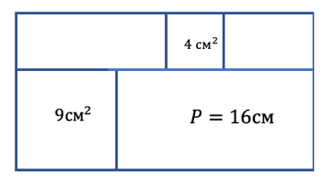
\includegraphics[scale=0.5]{kvadr.png}}
\end{figure}
\end{center}
Вася вырезал из бумаги два квадрата и три прямоугольника, а затем сложил из них большой прямоугольник (см. рисунок). Найдите площадь  полученного Васей прямоугольника, если площади квадратов равны $4\text{ см}^2$ и $9\text{ см}^2,$ а периметр одного из прямоугольников --- 16 см.\\
250. За какое время при движении против течения реки теплоход пройдёт 216 км, если его собственная скорость 15 км/ч, а скорость течения в 5 раз меньше собственной скорости теплохода?\\
251. За какое время при движении против течения реки теплоход пройдёт 204 км, если его собственная скорость 14 км/ч, а скорость течения в 7 раз меньше собственной скорости теплохода?\\
252. В некотором году в мае было пятниц больше, чем суббот. А какого числа в том году был второй вторник сентября?\\
253. В некотором году в мае было четвергов больше, чем пятниц. А какого числа в том году был второй вторник сентября?\\
254. В домике на шоссе живёт велосипедист Олег. Однажды он выехал из дома в магазин. Доехав до магазина, он сообразил, что забыл карточку, и поехал обратно в два раза быстрее. Он так сильно переживал, что проехал мимо своего дома некоторое расстояние. Повернув назад и ещё в два раза увеличив скорость, Олег успешно остановился у дома через 5 часов после того, как выехал из него. Сколько времени Олег ехал, удаляясь от своего дома? Ответ дайте в минутах.\\
255. В домике на шоссе живёт велосипедист Олег. Однажды он выехал из дома в магазин. Доехав до магазина, он сообразил, что забыл карточку, и поехал обратно в три раза быстрее. Он так сильно переживал, что проехал мимо своего дома некоторое расстояние. Повернув назад и ещё в три раза увеличив скорость, Олег успешно остановился у дома через 5 часов после того, как выехал из него. Сколько времени Олег ехал, приближаясь к своему дому? Ответ дайте в минутах.\\
256. Когда в Петербурге $12:12,$ то в Новосибирске $16:12.$ Когда в Новосибирске $12:15,$ то в Якутске $15:15.$ Самолёт вылетел из Якутска в Петербург в $13:15$ и летел 7 часов 40 минут. Во сколько он приземлился?\\
257. Когда в Петербурге $12:12,$ то в Екатеринбурге $14:12.$ Когда в Екатеринбурге $12:15,$ то в Хабаровске $17:15.$ Самолёт вылетел из Хабаровска в Петербург в $10:15$ и летел 8 часов 40 минут. Во сколько он приземлился?\\
258. Периметр прямоугольника равен 10 см. Чему равна площадь этого прямоугольника в квадратных сантиметрах, если его ширина равна 2 см?\\
259. Периметр прямоугольника равен 14 см. Чему равна площадь этого прямоугольника в квадратных сантиметрах, если его ширина равна 2 см?\\
260. Два пешехода одновременно вышли из магазина и пошли по прямой улице в противоположных направлениях. Скорость одного из них составляла 87 м/мин, скорость второго 98 м/мин. Какое расстояние будет между ними через 7 минут после выхода?\\
261. Два пешехода одновременно вышли из кафе и пошли по прямой улице в противоположных направлениях. Скорость одного из них составляла 76 м/мин, скорость второго 87 м/мин. Какое расстояние будет между ними через 9 минут после выхода?\\
262. Каток, имеющий форму прямоугольника, длина которого 57 м, а ширина 29 м, залит льдом, причём масса льда на одном квадратном метре катка составляет 10 кг. Найдите массу льда, покрывающего весь каток. Ответ выразите в килограммах.\\
263. Каток, имеющий форму прямоугольника, длина которого 47 м, а ширина 26 м, залит льдом, причём масса льда на одном квадратном метре катка составляет 10 кг. Найдите массу льда, покрывающего весь каток. Ответ выразите в килограммах.\\
264. На каждые 70 км пути машина расходует 6 л бензина. Сколько литров бензина потребуется, чтобы проехать 560 км?\\
265. На каждые 80 км пути машина расходует 7 л бензина. Сколько литров бензина потребуется, чтобы проехать 560 км?\\
266. Сколько квадратных дециметров в $800\text{ см}^2?$\\
267. Сколько квадратных дециметров в $600\text{ см}^2?$\\
268. 200 г конфет стоят 58 рублей. Сколько стоят 300 г таких конфет?\\
269. 300 г орехов стоят 87 рублей. Сколько стоят 200 г таких орехов?\\
270. На сколько секунд больше 5 минут 19 секунд, чем 3 минуты 48 секунд?\\
271. На сколько секунд больше 9 минут 23 секунды, чем 7 минут 57 секунд?\\
272. Птичка колибри во время полёта делает 1500 взмахов крыльями в минуту. Во время миграции колибри приходится лететь довольно далеко. Сколько взмахов крыльями делает колибри за полтора часа полёта?\\
273. Стрекоза во время полёта делает 1300 взмахов крыльями в минуту. Во время охоты стрекозе приходится много летать. Сколько взмахов крыльями делает стрекоза за полтора часа полёта?\\
274. Расстояние между двумя концами дорожки 32 м. Улитки ползут с разных концов дорожки навстречу друг другу. Скорость одной улитки 3 м/мин, скорость другой 4 м/мин. Каким будет расстояние между улитками через 7 минут, если они не будут останавливаться?\\
275. Расстояние между двумя концами дорожки 38 м. Две жужелицы ползут с разных концов дорожки навстречу друг другу. Скорость одной жужелицы 5 м/мин, скорость другой 4 м/мин. Каким будет расстояние между жужелицами через 6 минут, если они не будут останавливаться?\\
276. Нефтяной танкер привёз в порт 108000 галлонов нефти. Нефть из него выкачивают так, что за 2 часа объём нефти уменьшается на треть от того, который был в начале этих двух часов. Сколько галлонов нефти останется в танкере через 6 часов?\\
277. Молоковоз привёз на молокозавод 64000 пинт молока. Молоко из него сливают для переработки так, что за 3 часа объём молока уменьшается на четверть от того, который был в начале этих трёх часов. Сколько пинт молока останется в молоковозе через 9 часов?\\
278. Первая бегунья пробежала дистанцию 500 метров за 5 минут 10 секунд, а вторая бегунья пробежала дистанцию на 200 метров за 1 минуту 58 секунд. Если бы обе бегуньи бежали 400 метров каждая со своей скоростью, на сколько секунд вторая бегунья прибежала бы раньше, чем первая?\\
279. Первый бегун пробежал дистанцию 200 метров за 1 минуту 56 секунд, а второй бегун пробежал дистанцию 700 метров за 7 минут и 21 секунду. Если бы оба бегуна бежали 400 метров каждый со своей скоростью, на сколько секунд первый бегун прибежал бы раньше второго?\\
280. Два тигра за 4 часа могут съесть одну печеньку. Сколько тигров нужно, чтобы за 1 час съесть три печеньки?\\
281. Два тигра за 8 часов могут съесть одну печеньку. Сколько тигров нужно, чтобы за 1 час съесть две печеньки?\\
282. В течение 2021 года Катя покупала по одной конфете каждую субботу и каждый вторник, а в другие дни недели Катя не покупала конфет. Сколько конфет в 2021 году купила Катя, если 1 января 2021 года была пятница?\\
283. В течение 2021 года Катя покупала по одной конфете каждую пятницу и каждую среду, а в другие дни недели Катя не покупала конфет. Сколько конфет в 2021 году купила Катя, если 1 января 2021 года была пятница?\\
284. На первом складе было 480 кг конфет, а на втором --- в 3 раза больше. Все конфеты разложили в коробки по 12 кг в каждую. Одну четвёртую часть всех конфет отправили в магазин, а одну шестую часть остатка --- в детские сады. Сколько коробок с конфетами отправили в детские сады? Сколько коробок осталось?\\
285. Хоттабыч ехал на ослике 24 минуты, а потом летел на ковре-самолёте путь вдвое больший. Сколько времени он летел, если скорость ковра-самолёта в шесть раз больше, чем у ослика?\\
286. Если в Петербурге $12:12,$ то в Калининграде $11:12.$ Когда в Новосибирске $03:15,$ в Калининграде $22:15.$ Самолёт вылетел из Новосибирска в Москву в $13:20$ и летел 4 часа 40 минут. Во сколько он приземлился?\\
287. Если в Петербурге $12:12,$ то в Калининграде $11:12.$ Когда в Иркутске $04:15,$ в Калининграде $22:15.$ Самолёт вылетел из Иркутска в Москву в $10:20$ и летел 5 часов 40 минут. Во сколько он приземлился?\\
288. Вступительная олимпиада в 5 класс проводится в предпоследнее воскресенье мая. Каким по счёту днём года может быть день вступительной работы? Например, 1 февраля --- 32-й день года. Перечислите все возможные варианты.\\
289. Показ работ вступительной олимпиады в 5 класс проводится в предпоследний вторник мая. Каким по счёту днём года может быть день показа работ? Например, 1 февраля --- 32-й день года. Перечислите все возможные варианты.\\
290. На прямой дороге расположены три домика. Из них одновременно вышли три человека. Первый пошёл направо со скоростью 4 километра в час, а второй и третий --- налево со скоростью 3 и 5 километров в час соответственно. Первый встретил второго через 3 часа, а третьего --- через 3 часа 40 минут после выхода. Через какое время после встречи с первым третий догонит второго?\\
291. На прямой дороге расположены три домика. Из них одновременно вышли три человека. Первый пошёл направо со скоростью 3 километра в час, а второй и третий --- налево со скоростью 4 и 5 километров в час соответственно. Первый встретил второго через 3 часа, а третьего --- через 3 часа 15 минут после выхода. Через какое время после встречи с первым третий догонит второго?\\
292. Периметр прямоугольника равен 36 см. Если провести некоторый вертикальный разрез, то сумма периметров двух полученных прямоугольников будет равна 45 см. А чему будет равен периметр каждого из прямоугольников, если горизонтальным разрезом поделить исходный прямоугольник на два равных?\\
293. Периметр прямоугольника равен 38 см. Если провести некоторый вертикальный разрез, то сумма периметров двух полученных прямоугольников будет равна 45 см. А чему будет равен периметр каждого из прямоугольников, если горизонтальным разрезом поделить исходный прямоугольник на два равных?\\
294. Петя взял деревянный куб со стороной 60 см и распилил его на бруски размером $1\cdot2\cdot3$ дециметра. А Коля распилил такой же куб на бруски размером $6\times6\times12$см. У кого получилось больше брусков и на сколько?\\
295. Коля взял деревянный куб со стороной 60 см и распилил его на бруски размером $1\cdot2\cdot3$ дециметра. А Петя распилил такой же куб на бруски размером $6\times5\times10$см. У кого получилось больше брусков и на сколько?\\
296. Васины часы уходят вперёд на 15 минут в день, а часы Пети отстают на 10 минут в день. 1 мая в полдень на Васиных часах $17:00,$ а на Петиных $13:00.$ Какого числа и какого месяца впервые после 1 мая в полдень их часы покажут одинаковое время одновременно?\\
297. Васины часы уходят вперёд на 10 минут в день, а часы Пети отстают на 15 минут в день. 10 мая в полдень на Васиных часах $19:00,$ а на Петиных $15:00.$ Какого числа и какого месяца впервые после 10 мая в полдень их часы покажут одинаковое время одновременно?\\
298. Какой день недели будет через 10 дней, если послезавтра будет вторник?\\
299. Какой день недели будет через 10 дней, если позавчера была пятница?\\
300. Машина проезжает 18 метров за секунду. А сколько дециметров проедет машина за минуту?\\
301. Машина проезжает 17 метров за секунду. А сколько дециметров проедет машина за минуту?\\
302. Есть труба, в левый конец которой поступает вода со скоростью 1 литр за 35 секунд. Посередине трубы есть небольшая течь, поэтому вода вытекает из правого конца трубы со скоростью 1 литр за 36 секунд. Под место протекания поставили пустую литровую банку. За сколько минут наполнится банка?\\
303. Есть труба, в левый конец которой поступает вода со скоростью 1 литр за 44 секунд. Посередине трубы есть небольшая течь, поэтому вода вытекает из правого конца трубы со скоростью 1 литр за 45 секунд. Под место протекания поставили пустую литровую банку. За сколько минут наполнится банка?\\
304. Маша может добраться до школы за 38 минут, пройдя 25 минут пешком и проехав 13 минут на скейтборде. Также Маша может добраться до школы за 31 минуту, пройдя 11 минут пешком и проехав 20 минут на скейтборде. А сколько минут потребуется Маше, чтобы пройти весь путь до школы пешком?\\
305. Маша может добраться до школы за 40 минут, пройдя 26 минут пешком и проехав 14 минут на скейтборде. Также Маша может добраться до школы за 32 минуты, пройдя 10 минут пешком и проехав 22 минуты на скейтборде. А сколько минут потребуется Маше, чтобы пройти весь путь до школы пешком?\\
306. Поезд проехал 360 км за 5 часов с постоянной скоростью, после чего увеличил скорость на 9 км/ч и ехал ещё 3 часа. Сколько всего километров проехал поезд?\\
307. На одной дороге расположены город, посёлок и деревня (в таком порядке). Расстояние между посёлком и городом 20 км. Из города в деревню выезжает автобус, а через минуту после его старта из посёлка в деревню выезжает грузовик со скоростью 60 км/ч. Каждые 10 км автобус делает остановку на 1 минуту, а грузовик едет без остановок. Автобус догоняет грузовик через 1 час 40 минут после старта грузовика и в этот момент снова делает остановку на 1 минуту. Грузовик же продолжает ехать вперёд. Через какое время автобус во второй раз догонит грузовик? Каково расстояние от города до деревни, если от момента первой встречи грузовика и автобуса до прибытия автобуса в деревню прошло 34 минуты?\\
308. Дешёвая батарейка стоит в три раза дешевле дорогой. При этом в фонарике дешёвая батарейка работает 2 часа 37 минут, а дорогая работает 8 часов. Что прослужит дольше и на сколько минут --- три дешёвых батарейки или одна дорогая?\\
309. Дешёвая ручка стоит в четыре раза дешевле дорогой. При этом ей можно непрерывно писать 1 час 23 минуты, а дорогой ручкой можно писать 5 часов 30 минут. Что прослужит дольше и на сколько минут --- четыре дешёвых ручки или одна дорогая?\\
310. Периметр квадрата равен 32 см и составляет четверть периметра прямоугольника. Найдите площадь прямоугольника, если его ширина на 6 см меньше длины.\\
311. Периметр квадрата равен 54 см и составляет треть периметра прямоугольника. Найдите площадь прямоугольника, если его ширина на 9 см меньше длины.\\
312. Олег наполняет водой бассейн, имеющий форму параллелепипеда высотой 1 м, ширина и длина которого по 2 м. В одно ведро помещается $16\text{ дм}^3$ воды. Олег уже вылил в бассейн 40 вёдер. Какова глубина наполненной части бассейна? Выразите ответ в сантиметрах.\\
313. Лёша наполняет водой бассейн, имеющий форму параллелепипеда высотой 1 м, ширина и длина которого по 3 м. В одно ведро помещается $12\text{ дм}^3$ воды. Лёша уже вылил в бассейн 90 вёдер. Какова глубина наполненной части бассейна? Выразите ответ в сантиметрах.\\
314. Автобус движется между двумя городами с постоянной скоростью. Через 5 часов после начала движения ему остаётся проехать 450 км, а через 7 часов после начала движения остаётся 280 км. Найдите расстояние между городами.\\
315. Автобус движется между двумя городами с постоянной скоростью. Через 4 часа после начала движения ему остаётся проехать 385 км, а через 6 часов после начала движения остаётся 215 км. Найдите расстояние между городами.\\
316. На отрезке $AB$ отмечены точки $C$ и $K$ в таком порядке. Точка $E$ --- середина $AC,$ точка $P$ --- середина $KB.\ AB = 80$см; сумма $AE$ и $PB$ равна 19 см. Найдите длину $CK.$\\
317. На отрезке $MK$ отмечены точки $A$ и $B$ в таком порядке. Точка $O$ --- середина $AM,$ точка $C$ --- середина $KB.\ AB = 70$см; сумма $AO$ и $CB$ равна 14 см. Найдите длину $MK.$\\
318. Когда в городе Бубуду 1 час 32 минуты, в городе Дудубу 23 часа 32 минуты. Самолёт вылетает из Бубуду в 13 часов 45 минут по местному времени и приземляется в
Дудубу в 15 часов 20 минут по местному времени. Сколько длится полёт?\\
319. Когда в городе Тотомо 2 часа 13 минут, в городе Момото 23 часа 13 минут. Самолёт вылетает из Момото в 15 ч 20 мин по местному времени и приземляется в Тотомо в
23 ч 35 минут по местному времени. Сколько длится полёт?\\
320. Из прямоугольника со сторонами 12 см и 19 см вырезали прямоугольник со сторонами 7 см и 12 см. Оставшуюся часть разрезали на квадраты со стороной 1 см. Из всех них удалось сложить квадрат. Чему равна его площадь? Чему равна длина его стороны?\\
321. Из прямоугольника со сторонами 14 см и 22 см вырезали прямоугольник со сторонами
7 см и 16 см. Оставшуюся часть разрезали на квадраты со стороной 1 см. Из всех них удалось сложить квадрат. Чему равна его площадь? Чему равна длина его стороны?\\
322. Строительной бригаде надо огородить прямоугольный участок площадью $40\text{ м}^2.$ Для постройки забора они используют секции длиной 2 м. Каким может быть
наименьший периметр такого участка? Секции можно скреплять только концами. Ответ дайте в метрах.\\
323. Строительной бригаде надо огородить прямоугольный участок площадью $54\text{ м}^2.$ Для постройки забора они используют секции длиной 3 м. Каким может быть
наибольший периметр такого участка? Секции можно скреплять только концами. Ответ дайте в метрах.\\
324. Во сколько раз автомобиль, который едет со скоростью 60 км/ч, быстрее велосипедиста, едущего со скоростью 200 м/мин?\\
325. Во сколько раз автомобиль, который едет со скоростью 90 км/ч, быстрее велосипедиста, едущего со скоростью 300 м/мин?\\
326. Строители кладут плитку на пол в квадратной комнате. Сторона комнаты равна целому числу метров. Строители использовали 16 плиток 2 на 2 метра,
но некоторые не целиком. Какая могла быть максимальная площадь комнаты?\\
327. Строители кладут плитку на пол в квадратной комнате. Сторона комнаты равна целому числу метров. Строители использовали 9 плиток 2 на 2 метра,
но некоторые не целиком. Какая могла быть максимальная площадь комнаты?\\
328. Машина едет по длинному проспекту, на котором установлено 29 светофоров. Проспект начинается и заканчивается светофором. Светофоры зажигаются одновременно и горят зелёным 3 минуты для пешеходов, а затем 2 минуты 30 секунд для машин. Расстояние между соседними
светофорами автомобилист всегда проезжает за 1 минуту. Сколько времени понадобится машине, чтобы проехать весь проспект целиком? Машина начинает движение по проспекту сразу, как только загорается зелёный свет на первом светофоре.\\
329. Машина едет по длинному проспекту, на котором установлен 31 светофор. Проспект начинается и заканчивается светофором. Светофоры зажигаются одновременно и горят зелёным 2 минуты для пешеходов, а затем 3 минуты 30 секунд для машин. Расстояние между соседними светофорами автомобилист всегда проезжает за 1 минуту. Сколько времени понадобится машине, чтобы проехать весь проспект целиком? Машина начинает движение по проспекту сразу, как только загорается зелёный свет на первом светофоре.\\
330. Дан прямоугольник, длины сторон которого выражаются целым числом сантиметров. Оказалось, что можно отрезать от него прямоугольник периметра 420 см, и получится квадрат. Также оказалось, что можно приклеить к нему прямоугольник периметра 660 см, и получится квадрат. Придумайте такой прямоугольник, в ответ запишите обе его стороны.\\
331. Дан прямоугольник, длины сторон которого выражаются целым числом сантиметров. Оказалось, что можно отрезать от него прямоугольник периметра 420 см, и получится квадрат. Также оказалось, что можно приклеить к нему прямоугольник периметра 600 см, и получится квадрат. Придумайте такой прямоугольник, в ответ запишите обе его стороны.\\
332. В мае некоторого года суббот было больше, чем четвергов. Каким днём недели могло быть 30 января того года?\\
333. В мае некоторого года пятниц было больше, чем сред. Каким днём недели могло быть 30 января того года?\\
334. По круглому стадионе на самокате ездит тренер со скоростью 12 км/ч. Навстречу ему передвигается Максим с постоянной скоростью. Тренер заметил, что они постоянно встречаются в 4 разных точках этого круга. Чему может быть равна скорость Максима?\\
335. По круглому стадионе на самокате ездит тренер со скоростью 15 км/ч. Навстречу ему передвигается Максим с постоянной скоростью. Тренер заметил, что они постоянно встречаются в 4 разных точках этого круга. Чему может быть равна скорость Максима?\\
336. Параллелепипед $4\times4\times5$ облили краской и распилили на кубики со стороной 1. У скольких из полученных кубиков число окрашенных граней чётное?\\
337. Параллелепипед $4\times5\times5$ облили краской и распилили на кубики со стороной 1. У скольких из полученных кубиков число окрашенных граней чётное?\\
338. Сегодня 19 мая 2024 года. Какой будет месяц через 300 дней?\\
339. Сегодня 19 мая 2024 года. Какой будет месяц через 330 дней?\\
340. Когда в Брянске 10:17, в Хабаровске 17:17. Когда в Хабаровске 15:12, в Кургане 10:12. Путешественник выехал из Кургана в 12:01 и приехал на следующий день в Брянск в 03:46 местного времени. Сколько времени он путешествовал?\\
341. Когда в Брянске 10:17, в Хабаровске 17:17. Когда в Хабаровске 15:12, в Кургане 10:12. Путешественник выехал из Брянска в 13:23 и приехал на следующий день в Курган в 05:45 местного времени. Сколько времени он путешествовал?
\newpage
\section{Раздел 5: стандартные задачи}
1. В году 150 учебных дней. В каждом из четырёх классов решали по 4 задачи за один урок математики. Сколько всего задач было решено за год, если по субботам уроков математики не было, а во все остальные дни их было ровно по одному? (суббота также является учебным днём)\\
2. В году 150 учебных дней. В каждом из пяти классов решали по 3 задачи за один урок математики. Сколько всего задач было решено за год, если по субботам уроков математики не было, а во все остальные дни их было ровно по одному? (суббота также является учебным днём)\\
3. Доктор Айболит раздал четырём заболевшим зверям 2010 чудодейственных таблеток. Носорог получил на одну больше, чем крокодил, бегемот на одну больше, чем носорог, а слон --- на одну больше, чем бегемот. Сколько таблеток придётся съесть слону?\\
4. Доктор Айболит раздал четырём заболевшим зверям 2014 чудодейственных таблеток. Волк получил на одну меньше, чем лиса, медведь на одну меньше, чем волк, а рысь --- на одну меньше, чем медведь. Сколько таблеток придётся съесть рыси?\\
5. Какое число надо умножить на 10, чтобы результат был таким же, как при прибавлении к этому числу 18?\\
6. Какое число надо умножить на 9, чтобы результат был таким же, как при прибавлении к этому числу 24?\\
7. Как изменится разность, если уменьшаемое уменьшить на 8, а вычитаемое увеличить на 5?\\
8. Как изменится разность, если уменьшаемое увеличить на 11, а вычитаемое уменьшить на 5?\\
9. Хозяйка развела кур и кроликов. Всего у них 35 голов и 94 ноги. Сколько у хозяйки кур и сколько кроликов?\\
10. На ферме имеются гуси и коровы общим числом 30, а общее количество ног у них равно 86. Сколько на ферме гусей?\\
11. На ферме имеются гуси и коровы общим числом 40, а общее количество ног у них равно 98. Сколько на ферме коров?\\
12. Для похода 46 лицеистов приготовили шестиместные и четырёхместные лодки. Сколько было тех и других лодок, если все ребята разместились в 10 лодках и свободных мест не осталось?\\
13. Задумали число, увеличили его в 4 раза, а результат уменьшили в 6 раз. Получили 36. Какое число задумали?\\
14. Задумали число, увеличили его в 8 раз, а результат уменьшили в 12 раз. Получили 24. Какое число задумали?\\
15. В купейном вагоне 36 мест, по 4 в каждом купе. Укажите номер купе, в котором расположено место №23.\\
16. Из 23 школьников 17 изучают английский язык, а 11 --- немецкий язык. Сколько школьников изучают два языка, если известно, что каждый изучает хотя бы один язык?\\
17. Теплоход рассчитан на 750 пассажиров и 25 членов команды. Каждая спасательная шлюпка может вместить 70 человек. Какое наименьшее количество шлюпок должно быть на теплоходе, чтобы в случае необходимости в них можно было разместить всех пассажиров и членов команды?\\
18. В летнем лагере 218 детей и 26 воспитателей. В автобус помещается не более 45 пассажиров. Сколько автобусов потребуется, чтобы перевезти всех из лагеря в город?\\
19. В 4 классе 35 учеников. В течение учебного дня 20 человек питаются бутербродами, 11 человек посещают кафе, 10 человек голодают. Сколько человек съедает бутерброды, сидя в кафе?\\
20. В пиратской шайке 50 человек. Из них 32 одноруких, 29 одноглазых, 15 --- одноруких с одним глазом. Сколько здоровых пиратов в шайке?\\
21. В автобусе было несколько пассажиров. На первой остановке вышло 11 и вошло 6, а на второй вышло 7 и вошло 15 пассажиров. Сколько пассажиров было в автобусе до первой остановки, если после второй остановки автобуса их стало 40?\\
22. В автобусе было несколько пассажиров. На первой остановке вышло 7 и вошло 12, а на второй вышло 11 и вошло 8 пассажиров. Сколько пассажиров было в автобусе до первой остановки, если после второй остановки автобуса их стало 40?\\
23. Во время туристского слёта на питание 100 туристов израсходовали 32 кг мяса, что оказалось в 8 раз больше, чем масла, и в 2 раза меньше, чем хлеба. Сколько граммов каждого продукта в отдельности пришлось на питание одного туриста?\\
24. Во время школьного праздника на угощение 100 пятиклассников приготовили 24 кг мороженого, что оказалось в 8 раз больше, чем чая, и в 2 раза меньше, чем карамели. Сколько граммов каждого продукта в отдельности пришлось на угощение одного школьника?\\
25. В пачке 500 листов бумаги. За неделю в школе расходуется 1300 листов. Какое наименьшее количество пачек бумаги нужно купить в школу на 7 недель?\\
26. В пачке 500 листов бумаги. За неделю в школе расходуется 1100 листов. Какое наименьшее количество пачек бумаги нужно купить в школу на 9 недель?\\
27. Некоторое число таково, что прибавить к нему 4 --- то же самое, что умножить его на 3. Тогда умножить его на 6 --- это то же самое, что прибавить к нему...\\
28. Некоторое число таково, что прибавить к нему 6 --- то же самое, что умножить его на 3. Тогда умножить его на 5 --- это то же самое, что прибавить к нему...\\
29. Запишите шесть чисел подряд, если первое число равно 2, второе 3, а каждое следующее равно произведению двух предыдущих, увеличенному на 2.\\
30. Запишите шесть чисел подряд, если первое число равно 2, второе 5, а каждое следующее равно произведению двух предыдущих, уменьшенному на 3.\\
31. Аня, Боря и Витя обсуждали, у кого сколько карандашей. Петров с Сидоровым посовещались, и после этого Витя сказал: <<Если Иванова отдаст Петрову один карандаш, то у нас троих будет их поровну>>. На что Боря заметил: <<Если Аня отдаст все свои карандаши Вите, то у него будет ровно 10 карандашей>>. Определите фамилию и количество карандашей каждого из ребят.\\
32. Лёня, Максим и Нина обсуждали, у кого сколько ручек. Иванов с Сидоровым посовещались, и после этого Лёня сказал: <<Если Петрова отдаст Сидорову три ручки, то у нас троих будет их поровну>>. На что Максим заметил: <<Если Нина отдаст все свои ручки Лёне, то у него будет ровно 20 ручек>>. Определите фамилию и количество ручек каждого из ребят.\\
33. В лицее №239 два здания. Каждый день в лицее расходуется 260 листов бумаги, причём в первом здании на 6 листов больше, чем во втором. Сколько пачек бумаги надо закупить на 12 дней, если переносить открытые пачки и листы по улице нельзя, а в каждой пачке 500 листов бумаги?\\
34. В лицее №239 два здания. Каждый день в лицее расходуется 360 листов бумаги, причём в первом здании на 6 листов больше, чем во втором. Сколько пачек бумаги надо закупить на 12 дней, если переносить открытые пачки и листы по улице нельзя, а в каждой пачке 500 листов бумаги?\\
35. На столе лежат фрукты. Известно, что яблоко и апельсин вместе весят 167 граммов, апельсин и груша весят вместе 176 граммов, мандарин и апельсин весят вместе 200 граммов, а груша и яблоко весят вместе 159 граммов. Сколько весят вместе взятые мандарин, апельсин и груша?\\
36. На столе лежат фрукты. Известно, что апельсин и груша вместе весят 157 граммов, груша и мандарин весят вместе 175 граммов, яблоко и груша весят вместе 300 граммов, а мандарин и апельсин весят вместе 168 граммов. Сколько весят вместе взятые яблоко, мандарин и груша?\\
37. На дне рождения каждый мальчик съел 4 конфеты, 4 котлеты и 4 козинака, а каждая девочка съела 10 конфет, 3 котлеты и 24 козинака. Всего было съедено 714 конфет и 371 котлета Сколько было съедено козинаков?\\
38. На празднике каждый мальчик съел 5 мандаринов, 5 манго и 5 марципанов, а каждая девочка съела 11 мандаринов, 8 манго и 17 марципанов. Всего было съедено 813 мандаринов и 669 манго. Сколько было съедено марципанов?\\
39. В городах А и Б проходит олимпиада по математике. Известно, что в обоих городах олимпиада началась в 10 часов утра по местному времени и продолжалась одинаковое время. Оказалось, что в городе А олимпиада закончилась на час позже, чем началась в Б. При этом в Б она закончилась на 9 часов позже, чем началась в А. Сколько времени длится олимпиада?\\
40. В городах А и Б проходит олимпиада по математике. Известно, что в обоих городах олимпиада началась в 11 часов утра по местному времени и продолжалась одинаковое время. Оказалось, что в городе А олимпиада закончилась на час раньше, чем началась в Б. При этом в Б она закончилась на 7 часов позже, чем началась в А. Сколько времени длится олимпиада?\\
41. На складе лежат 30000 блоков массой по 33 кг каждый, и 3456 кирпичей по 2 кг каждый. Какое наименьшее количество машин грузоподъёмностью одна тонна надо, чтобы увезти это со склада?\\
42. На складе лежат 31000 блоков массой по 32 кг каждый, и 2345 кирпичей по 2 кг каждый. Какое наименьшее количество машин грузоподъёмностью одна тонна надо, чтобы увезти это со склада?\\
43. В трёх ящиках лежали 1001, 2999 и 239 гвоздиков. Мальчик Вася стал перекладывать гвоздики из ящика в ящик, при этом ничего не теряя. Когда Вася закончил, его мама выяснила, что теперь в первом ящике 4 гвоздика, а во втором 1007 гвоздиков. Сколько гвоздиков в третьем ящике?\\
44. В трёх ящиках лежали 2002, 1999 и 239 винтиков. Мальчик Вася стал перекладывать винтики из ящика в ящик, при этом ничего не теряя. Когда Вася закончил, его мама выяснила, что теперь в первом ящике 7 винтиков, а во третьем 1003 винтика. Сколько винтиков во втором ящике?\\
45. В течение недели ученик каждый день решал на две задачи больше, чем в предыдущий день, при этом в воскресенье он решил втрое больше задач, чем в понедельник. Сколько задач он решил в пятницу?\\
46. В течение недели ученик каждый день решал на две задачи больше, чем в предыдущий день, при этом в воскресенье он решил вчетверо больше задач, чем в понедельник. Сколько задач он решил в пятницу?\\
47. На дне озера бьёт родник. Стадо из 163 слонов могло бы выпить озеро за 1 день, а стадо из 33 слонов --- за 5 дней. За сколько дней выпьет озеро один слон?\\
48. На дне озера бьёт родник. Стадо из 158 слонов могло бы выпить озеро за 1 день, а стадо из 23 слонов --- за 7 дней. За сколько дней выпьет озеро один слон?\\
49. Дима и Максим хотят вместе заплатить 5600 рублей, разделив затраты поровну. Дима дал Максиму взаймы 10000 рублей, Максим заплатил 3200 рублей, а Дима --- оставшиеся деньги. Сколько денег должен дать Максим Диме, чтобы никто никому не был должен?\\
50. Вова и Максим хотят вместе заплатить 7800 рублей, разделив затраты поровну. Вова дал Максиму взаймы 3800 рублей, Вова заплатил 3200 рублей, а Максим --- оставшиеся деньги. Сколько денег должен дать Максим Вове, чтобы никто никому не был должен?\\
51. На дереве сидело несколько красных и несколько зелёных хамелеонов, а также несколько красных и несколько зелёных попугаев. Хамелеонов было 17, красных животных --- тоже 17, а зелёных животных было 14. После того как один из хамелеонов перекрасился из красного цвета в зелёный, красных попугаев и красных хамелеонов стало поровну. Сколько зелёных попугаев было на дереве?\\
52. На дереве сидело несколько красных и несколько зелёных хамелеонов, а также несколько красных и несколько зелёных попугаев. Хамелеонов было 15, зелёных животных --- тоже 15, а красных животных было 12. После того как один из хамелеонов перекрасился из красного цвета в зелёный, зелёных попугаев и зелёных хамелеонов стало поровну. Сколько красных попугаев было на дереве?\\
53. Гулливер погнался за лилипутом, когда расстояние между ними было равно 8 шагам Гулливера. Пока Гулливер делает 1 шаг, лилипут пробегает 7 шагов, но 1 шаг Гулливера равен 11 шагам лилипута. Сколько шагов пробежал лилипут до момента, когда Гулливер его догнал?\\
54. Гулливер погнался за лилипутом, когда расстояние между ними было равно 6 шагам Гулливера. Пока Гулливер делает 1 шаг, лилипут пробегает 7 шагов, но 1 шаг Гулливера равен 10 шагам лилипута. Сколько шагов пробежал лилипут до момента, когда Гулливер его догнал?\\
55. У Ани, Максима и Димы вместе 1410 монет, у Ани монет в 4 раза больше, чем у Максима, и на 3 монеты больше, чем у Димы. Сколько монет у Ани?\\
56. У Ани, Максима и Димы вместе 1401 монета, у Ани монет в 3 раза меньше, чем у Максима, и на 4 монеты больше, чем у Димы. Сколько монет у Ани?\\
57. Саша складывал два числа на калькуляторе, но, набирая второе число, случайно нажал в конце лишний ноль. Поэтому вместо 1222 он получил 5551. Какие числа хотел сложить Саша?\\
58. Паша складывал два числа на калькуляторе, но, набирая второе число, случайно нажал в конце лишний ноль. Поэтому вместо 1331 он получил 6641. Какие числа хотел сложить Паша?\\
59. Шесть мальчиков и четыре девочки организовали турнир в крестики-нолики. Каждый участник сыграл с каждым по одной партии. За выигрыш присуждали 2 очка, за ничью --- 1 очко, за проигрыш --- 0 очков. Девочки вместе набрали 40 очков. На сколько игр, в которых выиграла девочка у мальчика, больше, чем игр, в которых выиграл мальчик у девочки?\\
60. Шесть мальчиков и четыре девочки организовали турнир в крестики-нолики. Каждый участник сыграл с каждым по одной партии. За выигрыш присуждали 2 очка, за ничью --- 1 очко, за проигрыш --- 0 очков. Мальчики вместе набрали 40 очков. На сколько игр, в которых выиграла девочка у мальчика, больше, чем игр, в которых выиграл мальчик у девочки?\\
61. Возраст нескольких друзей составляет в сумме 62 года. Через 4 года он будет составлять 90 лет. Сколько этих друзей?\\
62. Для забора нужны доски длиной 75 сантиметров в количестве 112 штук. В магазине продаются доски длиной 4 метра. Сколько досок надо купить, чтобы построить забор?\\
63. Для забора нужны доски длиной 80 сантиметров в количестве 120 штук. В магазине продаются доски длиной 6 метра. Сколько досок надо купить, чтобы построить забор?\\
64. Света, Маша и Оля разделили между собой 80 конфет. Света заметила, что если она отдаст все свои конфеты Маше, то у Маши и Оли станет поровну конфет, а если она отдаст все свои конфеты Оле, то у Оли станет в четыре раза больше конфет, чем у Маши. Сколько конфет было у Светы?\\
65. Света, Маша и Оля разделили между собой 60 конфет. Света заметила, что если она отдаст все свои конфеты Маше, то у Маши и Оли станет поровну конфет, а если она отдаст все свои конфеты Оле, то у Оли станет в пять раз больше конфет, чем у Маши. Сколько конфет было у Светы?\\
66. Лифт в доме ездит с постоянной скоростью, а на каждом этаже, куда вызван, стоит одинаковое время. Время поездки в лифте считается от момента отправления с начального этажа до момента прибытия на конечный. Петя ехал вниз с 13 этажа, на 11 этаже к нему подсел Коля, на 7 этаже Таня, а на 5 этаже Витя. На первом этаже все вышли. Петя ехал 57 секунд, а Таня 25 секунд. Сколько секунд ехал Коля?\\
67. Лифт в доме ездит с постоянной скоростью, а на каждом этаже, куда вызван, стоит одинаковое время. Время поездки в лифте считается от момента отправления с начального этажа до момента прибытия на конечный. Петя ехал вниз с 11 этажа, на 9 этаже к нему подсел Коля, на 6 этаже Таня, а на 3 этаже Витя. На первом этаже все вышли. Петя ехал 54 секунды, а Таня 23 секунды. Сколько секунд ехал Коля?\\
68. У Олега есть 120 рублей. Тетрадь стоит 7 рублей 50 копеек, а ручка 12 рублей. Олегу обязательно нужно купить 3 ручки. Какое наибольшее количество тетрадей сможет купить Олег?\\
69. У Оли есть 140 рублей. Блокнот стоит 9 рублей 50 копеек, а линейка 14 рублей. Оле обязательно нужно купить 4 линейки. Какое наибольшее количество блокнотов сможет купить Оля?\\
70. У бедуина есть двугорбые и одногорбые верблюды. У всех верблюдов вместе 14 горбов и 44 ноги. Сколько одногорбых верблюдов у бедуина?\\
71. В цирке есть двугорбые и одногорбые верблюды. У всех верблюдов вместе 19 горбов и 48 ног. Сколько двугорбых верблюдов в цирке?\\
72. Кошка, собака и енот вместе весят 25 кг. Кошка и собака вместе весят 17 кг, енот и собака вместе весят 19 кг. Сколько весит собака?\\
73. Кролик, индюк и петух вместе весят 30 кг. Кролик и индюк вместе весят 22 кг, петух и кролик вместе весят 17 кг. Сколько весит кролик?\\
74. На фундаменте строят стену из кирпича. Когда четверть кирпичной кладки была завершена, высота её вместе с фундаментом была 1 м, когда половина всей кладки была закончена, высота была 160 см. Какой будет высота стены (с учётом фундамента), законченной на 2/3? Ответ выразите в сантиметрах.\\
75. В кадке, стоящей на полу, живёт пальма. Если привязать ленточку на высоте четверти пальмы от уровня кадки, то ленточка окажется на высоте 1 м 20 см от пола; если привязать ленточку в середине пальмы, то ленточка будет на высоте 190 см от пола. На какой высоте от пола будет ленточка, если она отмечает 2/5 высоты пальмы от уровня кадки? Ответ выразите в сантиметрах.\\
76. В магазине продаются свечки в виде цифр. Одинаковые цифры имеют одинаковую цену, а разные --- разную. Число 4385 стоит 36 динаров; число 27 стоит 17 динаров; число 56165 стоит 47 динаров; число 782 стоит 29 динаров; число 586 стоит 33 динара. Сколько стоит число 745231?\\
77. В магазине продаются свечки в виде цифр. Одинаковые цифры имеют одинаковую цену, а разные --- разную. Число 3276 стоит 36 гульденов; число 51 стоит 14 гульденов; число 49894 стоит 22 гульдена; число 715 стоит 22 гульдена; число 794 стоит 17 гульденов. Сколько стоит число 623158?\\
78. Балда и Емеля едят пирожки. Емеля может съесть 15 пирожков за полчаса, а Балда --- 15 пирожков за 20 минут. Чудо-печка каждые 2 минуты выпекает 3 пирожка. Печка пекла пирожки 2 часа. Успеют ли Емеля и Балда вместе съесть все пирожки за 2 часа?\\
79. Малыш и Карлсон едят плюшки. Малыш может съесть 4 плюшки за 15 минут, а Карлсон --- 16 плюшек за полчаса. Фрекен Бок каждые 4 минуты выпекает 3 плюшки. Она пекла плюшки 2 часа. Успеют ли Малыш и Карлсон вместе съесть все плюшки за 2 часа?\\
80. Кристофер Робин рассказывал Пятачку о диковинных животных, на которых ему приходилось охотиться: {\it <<Слонопотам в 5 раз тяжелее верблюмота, а кошкалот на 16 кг легче антиконды. При этом кошкалот и антиконда вместе весят столько же, сколько вместе слонопотам и верблюмот, хотя верблюмот на центнер легче слонопотама>>.} Сколько весит каждое из диковинных животных? Расположите их массы в порядке убывания.\\
81. Барон Мюнхгаузен рассказывал друзьям об удивительных птицах, обитающих за дальними морями:{\it <<Тётел в 6 раз легче мамугая, а пеликот на 34 кг тяжелее хвалибри. При этом тётел и мамугай вместе весят столько же, сколько вместе пеликот и хвалибри, хотя тётел на полцентнера легче мамугая>>.} Сколько весит каждая из удивительных птиц? Расположите в ответе их массы в порядке возрастания.\\
82. Сумма уменьшаемого, вычитаемого и разности равна 36. Найдите уменьшаемое.\\
83. У Зои было на 200 фантиков больше, чем у Оли. Сколько фантиков Зоя должна дать Оле, чтобы у них стало одинаковое количество фантиков?\\
84. На первой остановке в автобус вошли 8 человек. А на каждой следующей выходили 5 человек, а входили 7 человек. Сколько пассажиров было в  автобусе между третьей и четвёртой остановкой?\\
85. На острове 486 домов. В каждом доме живёт по 5 зайцев, у каждого зайца по 3 зайчика. Сколько зайцев и зайчиков живёт в этих домах? Напишите только выражение, вычислять его значение НЕ надо.\\
86. В парке 4008 насекомых. Половина из них пчёлы, одна треть --- мухи, четвёртая часть остальных ---  гусеницы. Сколько в парке гусениц?\\
87. Жители планеты Нрутас имеют либо 1 голову и 4 руки, либо 2 головы и 3 руки. Делегация с этой планеты на Землю имеет на всех 11 голов и 29 рук. Сколько всего нрутасианцев в делегации?\\
88. Жители планеты Нутпен имеют либо 1 голову и 3 ноги, либо 3 головы и 2 ноги. Делегация с этой планеты на Марс имеет на всех 11 голов и 19 ног. Сколько всего нутпенсианцев в делегации?\\
89. Олег хочет купить другу Мише подарок на день рождения. Он знает, что Миша хочет синий грузовик. В магазине продаётся 19 машинок, 12 из которых синие, 11 --- грузовики. Из какого минимального количества синих грузовиков Олег точно может выбрать подходящий подарок?\\
90. Алиса хочет купить подруге Тане подарок на день рождения. Она знает, что Таня хочет книгу сказок с картинками. В магазине продаётся 23 книги, 10 из которых со сказками, 17 --- с картинками. Из какого минимального количества книг сказок с картинками Алиса точно может выбрать подходящий подарок?\\
91. Чайка ловила рыбу --- корюшку, ряпушку, плотву и уклейку. За неделю она поймала 256 рыбок, причём корюшки и ряпушки вместе втрое меньше, чем плотвы и уклейки вместе. Корюшки она поймала на 12 рыбок больше, чем ряпушки, а уклеек в 7 раз меньше, чем плотвы. Выясните, каких рыбок --- корюшки или уклеек чайка поймала больше и на сколько?\\
92. Дракон таскал в своё логово драгоценные камни --- рубины, алмазы, изумруды и сапфиры. Рубинов и алмазов вместе оказалось вдвое больше, чем изумрудов и сапфиров вместе. Всего камней было 351. Алмазов было в 5 раз меньше, чем рубинов, а сапфиров на 7 больше, чем изумрудов. Выясните, чего было больше --- алмазов или изумрудов и на сколько?\\
93. Четыре подруги (Катя, Лена, Маша, Нина) решили сварить компот из 36 груш. Катя купила 11 груш, Лена --- 10 груш, Маша --- 15 груш (все груши стоили одинаково). Нина принесла 216 рублей. Сколько рублей кому из девочек она должна отдать?\\
94. Четверо друзей (Антон, Вадим, Борис, Гена) решили сварить компот из 32 яблок. Антон купил 9 яблок, Борис --- 10 яблок, Вадим --- 13 яблок (все яблоки стоили одинаково). Гена принёс 128 рублей. Сколько рублей кому из мальчиков он должен отдать?\\
95. Собирались раскрасить 27 тарелок. Четыре тарелки разбили, пока везли. Все остальные были раскрашены красным, синим или обоими цветами сразу. Синим раскрасили 18 тарелок, красным --- 21 тарелку. Сколько тарелок раскрасили обоими цветами одновременно?\\
96. Рыцарь и 5 драконов весят столько же, сколько дракон и 8 рыцарей. Сколько рыцарей потребуется, чтобы уравновесить 8 драконов?\\
97. Диван и собачонка вместе весят 46 кг, чемодан и корзина --- 17 кг, собачонка и корзина --- 11 кг, диван и чемодан --- 52 кг. Сколько весят вместе диван, чемодан, корзина и собачонка?\\
98. Четвероклассник Коля Рисовалкин коллекционирует карандаши. У него в коллекции 68 --- синих, зелёных, жёлтых и красных. Синих карандашей в 14 раз больше, чем жёлтых, и на 6 штук меньше, чем зелёных. Количество красных карандашей составляет седьмую часть синих. Сколько карандашей какого цвета есть у Коли?\\
99. На дереве сидело 18 попугаев. Из них 10 --- не зелёные, а 9 --- крикливые. Когда прилетел ещё один попугай, зелёных оказалось столько же, сколько крикливых. Был ли прилетевший попугай зелёным? Крикливым?\\
100. Средней ценой купленного товара называют количество потраченных на весь товар денег, делённое на количество купленного товара. Даша купила на 480 руб. тетрадок. Половину денег она потратила на тетрадки по 60 руб. за штуку, а другую половину на тетради, цена которых вдвое меньше. Какова средняя цена тетрадок, купленных Дашей?\\
101. У числа 2019 перемножьте все ненулевые цифры и прибавьте 5 (например, для числа 10234 эта операция даст $1\cdot2\cdot3\cdot4+5=29).$ С получившимся числом проделайте те же операции. И так до тех пор, пока не получится однозначное число. Какое это будет число?\\
102. У числа 2017 перемножьте все ненулевые цифры и прибавьте 5 (например, для числа 10234 эта операция даст $1\cdot2\cdot3\cdot4+5=29).$ С получившимся числом проделайте те же операции. И так до тех пор, пока не получится однозначное число. Какое это будет число?\\
103. Карлсон ест торт со скоростью 200 граммов в минуту,а Малыш --- 25 граммов в минуту. Карлсон начал есть торт. Через минуту к нему присоединился Малыш, а ещё через четыре минуты торт закончился. Сколько весил этот торт?\\
104. Винни Пух ест мёд со скоростью 300 граммов в минуту, а Пятачок --- 20 граммов в минуту. Винни Пух и Пятачок начали есть горшочек с мёдом вместе. Через пять минут Пятачка отозвал Кролик, и Винни Пух продолжил обедать один. А ещё через минуту мёд закончился. Сколько мёда было в горшочке?\\
105. На автобусную экскурсию захотели поехать 174 мальчика, 148 девочек и 14 учителей. Каждый автобус вмещает 45 пассажиров. Сколько автобусов потребуется, чтобы смогли поехать все желающие?\\
106. На автобусную экскурсию захотели поехать 136 мальчика, 194 девочек и 15 учителей. Каждый автобус вмещает 45 пассажиров. Сколько автобусов потребуется, чтобы смогли поехать все желающие?\\
107. На ферме содержатся козы, гуси и лошади. Оказалось, что у них голов столько же, сколько крыльев, а рогов на восемь меньше, чем голов. Сколько лошадей на ферме?\\
108. На ферме содержатся коровы, лошади и утки. Оказалось, что у них голов столько же, сколько рогов, а крыльев на десять меньше, чем голов. Сколько лошадей на ферме?\\
109. Когда Маше было пять лет, Косте было столько же лет, сколько Тане год назад. Что больше --- возраст Кости или сумма возрастов Тани и Маши, и на сколько?\\
110. Через год Ксюше будет столько же лет, сколько исполнилось Антону, когда Насте было семь лет. Что больше --- возраст Антона или сумма возрастов Ксюши и Насти, и на сколько?\\
111. Тане и Андрею вместе 21 год. Когда Андрею было столько, сколько Тане сейчас, им вместе было 15 лет. Сколько лет было тогда Андрею?\\
112. Даше и Ксюше 18 лет. Когда Даше было столько лет, сколько Ксюше сейчас, им вместе было 10 лет. Сколько лет тогда было Ксюше?\\
113. Бабушка Оля в 9 раз старше внучки Тани, а мама Аня младше бабушки Оли на столько же лет, на сколько мама Аня старше внучки Тани. Вместе бабушке, маме и внучке 90 лет. Сколько лет бабушке Оле?\\
114. Хоттабыч --- древний волшебник. Когда он творит заклинание, он выдёргивает из своей бороды волосок, рвёт его на две части и говорит <<Трах-тибидох!>>. В будние дни Хоттабыч творит по 3 заклинания, а в субботу и воскресенье --- по 5. Сейчас утро понедельника, а в бороде Хоттабыча 2019
волосков. Через сколько дней эти волоски закончатся?\\
115. Хоттабыч --- древний волшебник. Когда он творит заклинание, он выдёргивает из своей бороды волосок, рвёт его на две части и говорит <<Трах-тибидох!>>. В будние дни Хоттабыч творит по 2 заклинания, а в субботу и воскресенье --- по 7. Сейчас утро понедельника, а в бороде Хоттабыча 2019
волосков. Через сколько дней эти волоски закончатся?\\
116. Путник поднимается в гору по лестнице, в которой 2019 ступеней. Как правило, он шагает через ступеньку, но после десяти таких шагов он отдыхает и делает три шага, не перешагивая ступеньки. Сколько шагов сделал путник?\\
117. На уроке рисования Алёна вырезала из клетчатой бумаги прямоугольник $20\times18$ клеток. Сидевший с ней Богдан случайно капнул на него синей краской, после чего ровно треть клеток оказались запачканными. После этого, снова случайно, он пролил на него жёлтую краску. В результате оказалось, что клеток только с синими пятнами ровно в два раза меньше, чем клеток только с жёлтыми пятнами. Докажите, что чистых клеток ровно в два раза больше, чем сине-жёлтых (чистые клетки --- это клетки, на которых нет пятен краски, а сине-жёлтые --- это клетки, на которых есть и синие, и жёлтые пятна).\\
118.  На уроке рисования Алёна вырезала из клетчатой бумаги прямоугольник $20\times20$ клеток. Сидевший с ней Богдан случайно капнул на него синей краской, после чего ровно четверть клеток оказались запачканными. После этого, снова случайно, он пролил на него жёлтую краску. В результате оказалось, что клеток только с синими пятнами ровно в три раза меньше, чем клеток только с жёлтыми пятнами. Докажите, что чистых клеток ровно в три раза больше, чем сине-жёлтых (чистые клетки --- это клетки, на которых нет пятен краски, а сине-жёлтые --- это клетки, на которых есть и синие, и жёлтые пятна).\\
119. Дениска, Мишка и Алёнка собрали марки. Изучая свои альбомы, дети обнаружили: 1) у каждого коллекционера в альбоме нет одинаковых марок; 2) у Дениски и Мишки марок поровну, но нет ни одной одинаковой; 3) у Дениски и Алёнки одинаковых марок ровно столько, сколько уникальных марок у Мишки; 4) у Алёнки нет уникальных марок. Докажите, что у Алёнки марок столько же, сколько у Дениски.\\
120. Коля купил 2 пирожных, 4 йогурта и 2 шоколадных батончика, а Антон купил 1 йогурт, 3 шоколадных батончика и 3 пирожных. Сколько стоит йогурт, если Коля за свои покупки заплатил 440 рублей, а Антон --- 560?\\
121. Возраст нескольких друзей в сумме составляет 62 года. Через 3 года он будет составлять 80 лет. Сколько этих друзей?\\
122. У полковника 10 майоров, у каждого майора 10 лейтенантов, у каждого лейтенанта 10 солдат. Какова численность войска (всех званий)?\\
123. Саша складывал два числа на калькуляторе, но, набирая второе число, случайно нажал в конце лишний ноль. Поэтому вместо 1331 он получил 8000. Какие числа хотел сложить Саша?\\
124. Автомобиль ехал по дороге Москва-Петербург, начало его пути у столба <<104-й км>>, конец пути у столба <<204-й км>>. Проехав четверть пути, автомобиль сломался. Около какого столба сломался автомобиль?\\
125. У Ани, Бори и Вити вместе 38 монет, у Ани монет в 4 раза больше, чем у Бори, и в 3 раза больше, чем у Вити. Сколько монет у Ани?\\
126. После ремонта в пустую гостиницу приехали китайские туристы и заняли половину всех номеров. Затем в половине оставшихся поселились японские туристы, а последними в гостиницу приехали французы и заняли треть номеров, оставшихся после заселения японцев. Сколько номеров в гостинице, если французы живут в трёх номерах?\\
127. Для покупки семи шоколадок Саше не хватает 35 рублей. Если он купит шесть шоколадок, то у него останется 15 рублей. Сколько шоколадок он сможет купить на 610 рублей?\\
128. Чтобы купить девять открыток, Ире не хватает 14 рублей. Если она купит восемь открыток, то у неё останется 26 рублей. Сколько открыток она сможет купить на 700 рублей?\\
129. Поспорили как-то три зимних месяца: кто из них самый холодный. Ударили месяцы посохами оземь и заморозили все деревья в лесу. Январь заморозил сразу 34 дерева, что оказалось в 2 раза меньше, чем декабрь, а Февраль на 17 больше, чем декабрь. Посчитайте, сколько всего деревьев было в лесу.\\
130. Мальчик и девочка носят воду вёдрами из колодца. Бочка в 70 л наполнится, если мальчик выльет в неё 5 своих полных вёдер, а девочка добавит к ним 6 своих.
Бочка в 83 л наполнится, если мальчик выльет а неё 6 своих полных вёдер, а девочка добавит к ним 7 своих. Сколько раз им надо вместе сходить за водой, чтобы бочка в 90 л оказалась полной?\\
131. Три подружки решили коллекционировать марки. Лена собрала 22 марки, что на 16 больше, чем Соня. Соня собрала марок в 2 раза меньше, чем Юля. Сколько марок собрали девочки вместе?\\
132. Три хозяйки Маша, Катя и Надя солили огурцы на зиму в одинаковых банках. Маша засолила 27 банок, что в 2 раза меньше, чем засолила Катя. Надя заготовила на 4 банки больше, чем Маша и Катя вместе. Сколько банок огурцов засолили хозяйки вместе?\\
133. У Никиты есть детали только для одного робота. Никита собирает робота за 3 мин 44 с, а разбирает его за 1 мин 16 с. Его младший брат Гена нехотя съел суп, посмотрел 3 мин в окно, потом выпил компот, затратив на всё вместе 19 мин. Причём на суп Гена затратил на 12 мин больше, чем на компот. Сколько раз Никита успел бы собрать своего робота, пока Гена ел суп, если бы работал без остановки?\\
134. У продавца было 28 ящиков с грушами, по 4 кг в каждом. К концу рабочего дня оказалось, что продано на 8 кг груш больше, чем осталось. Сколько ящиков груш было продано?\\
135. У фермера было 26 мешков с морковью по 7 кг в каждом. К концу недели оказалось, что фермер продал на 14 кг моркови больше, чем у него осталось. Сколько мешков моркови было продано?\\
136. В питомнике вырастили саженцы деревьев: клёнов было 287, а на кажые 7 клёнов приходилось 14 елей и 12 дубов. Сколько всего саженцев вырастили в питомнике?\\
137. Двум мастерицам фабрики игрушек поручили сделать 40 глиняных лошадок и 54 павлина. Ольга тратит на любую игрушку по 5 минут. Татьяна лепит лошадку за 4 минуты, а павлина за 6 минут. Придумайте, как мастерицам распределить работу, чтобы, работая вдвоём, закончить её как можно скорее. Найдите, сколько времени потребует ваш способ. Объяснять, почему он самый лучший, не надо.\\
138. Егор живёт в шестнадцатиэтажном доме в квартире №274. В каждом подъезде на каждом этаже расположено по шесть квартир. На каком этаже живёт Егор?\\
139. Лиза раскладывает апельсины по корзинам. Если она положит по пять апельсинов в каждую корзину, останется три лишних апельсина. А если класть по шесть апельсинов в корзину, останутся три лишние корзины. Сколько апельсинов у Лизы?\\
140. У 28 человек 5 <<Ы>> класса на собрание пришли папы и мамы. Мам было 24, пап 18. У скольких учеников на собрание пришли одновременно и папа, и мама?\\
141. Коле Гераскину 12 лет, а профессору Селезнёву 42. Через сколько лет Коля будет вдвое младше профессора?\\
142. Ученик Вовочка любит решать математические задачи. Известно, что вчера он решил на 11 задач меньше, чем позавчера, и на 32 задачи меньше, чем позавчера и сегодня вместе. Сколько задач решил Вовочка сегодня?\\
143. На корабле <<Пиратское счастье>> несколько кошек, матросов, как и одноногий капитан. У всех вместе взятых 15 голов и 41 нога. Сколько на корабле было кошек?\\
144. Тилли, Вилли и Дилли участвовали в легкоатлетическом забеге. В какой-то момент времени оказалось, что они бегут рядом друг с другом, впереди них бежит половина участников забега и позади них треть участников забега. Сколько спортсменов участвовало в забеге?\\
145. Алёша задумал число. Он прибавил к нему 5, потом разделил сумму на 3, умножил на 4, отнял 6, разделил на 7 и получил число 2. Какое число задумал Алёша?\\
146. Гриша с папой ходил в тир. Уговор был такой: Гриша делает 5 выстрелов и за каждое попадание в цель получает право сделать ещё два выстрела. Всего Гриша сделал 17 выстрелов. Сколько раз Гриша попал в цель?\\
147. Во сколько раз секундная стрелка движется быстрее часовой?\\
148. Банк имеет неограниченное число купюр достоинством 3 и 5 рублей.  Докажите, что Банк может выдать без сдачи любое число рублей, начиная с 8 руб.\\
149. Во дворе ходят собаки и куры. У всех животных вместе 34 ноги и 11 голов. Сколько на дворе кур и сколько собак?\\
150. У Феди было 560 г орешков. После того, как мальчик съел часть из них, он посчитал, что если бы он съел ещё 29 г орешков, то у него бы осталось $\cfrac{2}{7}$ всех орешков. Найдите, сколько граммов орешков съел Федя.\\
151. Год назад маме было столько же лет, сколько месяцев было сыну. Сейчас им в сумме 41 год. Сколько лет каждому из них?\\
152. Винни шёл от Кролика домой  ел мёд. На середине пути он обнаружил, что съел треть мёда, и решил, что может есть вдвое быстрее. Пройдя ещё половину оставшегося пути, Винни решил развернуться и скорее пойти к Кролику за ещё одним горшком мёда. Винни пошёл вдвое быстрее, чем раньше. Хватит ли ему мёда до домика Кролика, если скорость поедания мёда он не менял? Поясните ответ.\\
153. В математической олимпиаде для марсиан 5 задач, за каждую дают от 1 до 20 баллов. То есть 0 баллов набрать нельзя! При этом в зачёт идёт только 4 лучших задачи из 5. Марсианин Йумпага набрал за 5 задач 72 балла. Какое наименьшее количество баллов ему может пойти в зачёт?\\
154. Четверо товарищей покупают лодку. Первый вносит половину суммы, вносимой остальными, второй треть суммы, вносимой остальными, третий четверть суммы, вносимой остальными, а четвёртый 130 рублей. Сколько стоит лодка?\\
155. В трёх шкафах 2580 книг. В первом шкафу 350 книг. В третьем шкафу книг в 3 раза  больше, чем в первом и во втором шкафу, вместе взятых. Сколько книг во втором шкафу?\\
156. Три девочки – Оля, Ира и Аня – собирали на поле васильки. Ира собрала 28 васильков, Аня собрала в 2 раза больше васильков, чем Оля и Ира вместе взятые. Сколько васильков собрала Оля, если всего девочки собрали 150 васильков?\\
157. У Винни-пуха в погребе стоят бочонки с липовым и цветочным мёдом. В них 95 кг мёда, причём цветочного на 15 кг меньше, чем липового. Каждый бочонок вмещает 5 кг мёда. Сколько бочонков с липовым мёдом в погребе? А сколько с цветочным?\\
158. Бабушка наварила летом 39 литров варенья --- малинового и клубничного. Клубничного варенья оказалось на 9 литров меньше, чем малинового. Всё варенье разлито в трёхлитровые банки. Сколько банок с клубничным вареньем получилось у бабушки? И сколько с малиновым?\\
159. Трое ребят поделили между собой 176 рублей. Причём Коля получил на 34 рубля больше Жени, а Митя столько же, сколько Женя и Коля вместе. Сколько кому досталось?\\
160. Миша, Гриша и Алёша собирали грибы. Миша и Гриша вместе набрали 36 грибов. Гриша и Алёша на двоих собрали 42 гриба. А Миша и Алёша вдвоем набрали ровно 50 грибов. Сколько грибов набрал каждый мальчик по отдельности?\\
161. Мастер и два его помощника 3 часа 12 минут одновременно ремонтировали чайники. Первый помощник отремонтировал на 3 чайника больше второго и на 6 чайников меньше мастера. Сколько времени потратил каждый помощник и мастер на ремонт одного чайника, если второй помощник отремонтировал в 4 раза меньше чайников, чем мастер?\\
162. В зоомагазине продают больших и маленьких птиц. Большая птица стоит вдвое дороже маленькой. Одна дама купила 5 больших птиц и 3 маленьких, а другая – 5 маленьких и 3 больших. При этом первая дама заплатила на 20 рублей больше. Сколько стоит каждая птица?\\
163. В школьной библиотеке имеется 273 учебника по алгебре, что в 27 раз меньше, чем учебников по остальным предметам. Невоспитанные дети разрисовали $\cfrac{5}{6}$  учебников. Сколько чистых учебников осталось в библиотеке?\\
164. Библиотекарь протёр пыль с 360 книг, что составляет $\cfrac{3}{4}$ всех книг библиотеки. Сколько в библиотеке исторических романов, если они составляют $\cfrac{2}{5}$ от всего числа книг?\\
165. В школьных соревнованиях по лыжным гонкам, беге на коньках и игре в хоккей участвовали 696 человек. Лыжники составляли $\cfrac{1}{3}$ всех участников, конькобежцы --- $\cfrac{1}{4}$ от числа остальных спортсменов. Сколько детей играли в хоккей?\\
166. Кум Тыква накопил к старости 320 кирпичей и решил построить из них дом. В первый день он выложил четверть всех кирпичей и ещё 12 штук. Во второй день он выложил треть оставшихся кирпичей и ещё 7 штук. В третий день, выложив оставшиеся кирпичи, он достроил дом. Сколько кирпичей положил он в последний день?\\
167. Вася принес из леса 80 грибов: подберезовики, подосиновики и белые. Белых была $\cfrac{1}{5}$ часть, четверть остальных составляли подосиновики, а все прочие --- это подберёзовики. Сколько подберёзовиков нашел Вася?\\
168. На олимпиаде половина участников решила ровно 2 задачи, четверть участников --- ровно 3 задачи, а остальные 10 человек решили по 5 задач. Сколько всего ребят участвовало в олимпиаде?\\
169. Два робота круглосуточно собирают пылесосы. Робот <<Винтик>> собирает 16 пылесосов за 15 часов, а робот <<Шпунтик>> собирает 16 пылесосов за сутки. Роботов включили одновременно. Сколько пылесосов они соберут вместе за 30 часов? За какое время они вместе соберут 104 пылесоса?\\
170. Юра делает 120 бумажных корабликов за 3 часа, а Вася делает 120 бумажных корабликов за 2 часа. Сколько времени им нужно, чтобы вместе сделать 25 бумажных корабликов? Сколько бумажных корабликов они вместе сделают за 5 часов?\\
171. Мама чистит ведро картошки за 10 минут, папа за 12 минут, а Вася за 1 час. За сколько времени они почистят ведро картошки, работая вместе?\\
172. Винни-Пух съедает банку меда за 10 минут, а Пятачок --- за 15. За какое время они съедят 7 банок меда, если будут есть одновременно?\\
173. Коротышки пекли блины. Пончик может испечь 90 блинов за 45 минут, а Торопыжка --- за 30 минут. Незнайка может испечь столько же блинов, сколько за минуту пекут Пончик и Торопыжка вместе. За сколько минут Незнайка может испечь 90 блинов?\\
174. Малыш может съесть 600 г варенья за 6 минут, а Карлсон --- в 2 раза быстрее. За какое время они съедят это варенье вместе?\\
175. Собака выпьет миску молока за 5 минут, а кошка за 20 минут. За сколько минут они выпьют молоко вместе?\\
176. Через маленькое отверстие вода из бака выльется за 30 минут, а через большое --- за 6 минут. За сколько минут выльется вода из бака через оба отверстия одновременно?\\
177. Кошка Мурка съедает банку <<Вискас>> за 6 минут, а кот Васька --- в 2 раза быстрее. За какое время они съедят банку <<Вискас>> вместе?\\
178. Малыш съедает 900 г варенья за 9 минут. Карлсон делает это вдвое быстрее. За сколько минут они вместе съедят  1 кг 800 г варенья?\\
179. Лена  может собрать корзину клубники за час, а её старшая сестра в 2 раза быстрее, за сколько минут сестры соберут корзину ягод вместе?\\
180. Токарь вытачивает 72 одинаковые детали за 3 ч, а его ученику на выполнение этой работы требуется в 2 раза больше времени. За сколько часов они выточат 72 детали, работая вместе?\\
181. Чебурашка съест вагон апельсинов за 56 дней, а крокодил Гена за 8 дней. За сколько дней они съедят вагон апельсинов вместе?\\
182. На празднике 22 ученика. У каждого мальчика по 3 шара, у каждой девочки по 5 шаров. Всего надули 86 шаров. Кого на празднике больше --- девочек или мальчиков и на сколько?\\
183. В гараже стоят 750 автомобилей. Грузовые автомобили имеют по 6 колёс, а легковые --- по 4 колеса. Каких автомобилей в гараже больше и на сколько, если колёс всего 3024?\\
184. В порту стоят яхты с одной мачтой и шхуны с 2 мачтами. Старенький смотритель порта забыл, сколько шхун и сколько яхт находится в порту. Только помнит, что всего пришло ровно 100 кораблей. Помоги ему восстановить данные, если он насчитал в порту всего 146 мачт.\\
185. В комнате 10 столов. Часть из них с одним выдвижным ящиком, а часть с двумя. Всего в столах 14 ящиков. Сколько столов с одним ящиком и сколько с двумя?\\
186. На прогулку пошли четвероклассники и пятиклассники. Все они были либо босиком, либо в тапочках. Четвероклассников было 24, а босых учеников 16. Обутых пятиклассников было столько же, сколько босых четвероклассников. Сколько учеников  ходили на прогулку?\\
187. В классе 27 пловцов, 10 борцов и 15 футболистов. Каждый спортсмен занимается ровно двумя из этих видов спорта. Сколько всего в классе спортсменов?\\
188. В классе 17 пловцов, 6 борцов и 13 футболистов. Каждый спортсмен занимается ровно двумя из этих видов спорта. Сколько всего в классе спортсменов?\\
189. В саду у Ани и Вити росло сто розовых кустов. Витя полил половину всех кустов, и Аня полила половину всех кустов. При этом оказалось, что ровно три куста, самые красивые, были политы и Аней, и Витей. Сколько розовых кустов остались неполитыми?\\
190. В каждый из четырех походов ходила группа из 20 человек. Во все 4 похода ходили 10 человек. Ровно в 3 похода ходили 9 человек. Ровно в 2 похода ходили 5 человек. Сколько человек ходило только в 1 поход?\\
191. В секции плавания занимается 48 детей. Треть из них --- девочки. Ровно четверть детей ездила на сборы. Известно, что ровно 9 девочек на сборы не ездили. Сколько мальчиков не ездили на сборы?\\
192. Каждый из 35 четвероклассников является читателем по крайней мере одной из двух библиотек: школьной и районной. 25 человек берут книги в школьной библиотеке, 20 --- в районной. Сколько четвероклассников являются читателями обеих библиотек?\\
193.  К репетитору по математике ходит 24 учеников. Из них олимпиадные задачи любят решать 6 человек, обычные и олимпиадные – 2 человека, а 3 ученика вообще не любят решать задачки. Сколько у репетитора по математике тех учеников, которые любят решать только обычные задачи?\\
194. В магазин привезли одинаковое количество ящиков с бананами и апельсинами. Всего 96 кг.  Один ящик с бананами тяжелее, чем ящик с апельсинами на 2 кг, и их общий вес на 24 кг больше, чем вес апельсинов. Сколько ящиков бананов и сколько  ящиков апельсинов привезли? Сколько килограммов бананов в одном ящике? Сколько килограммов апельсинов?\\
195. В одной рукописи было 240 страниц, в другой --- 320 страниц, в третьей --- 480 страниц. Третью рукопись пришлось перепечатывать на 4 дня дольше, чем вторую. Сколько потребовалось дней, чтобы при одной и той же производительности труда перепечатать все три рукописи?\\
196. Маша купила больше Вари на 6 шоколадок и потратила на 300 рублей больше. Всего было куплено 10 шоколадок. Сколько потратила каждая девочка на шоколад?\\
197. Иван разделил 360 на задуманное число. Из результата вычел 17, затем умножил на 3 и прибавил 21. Получилось 105. Какое число задумал Иван?\\
198. Игорь задумал число и вычел из него 8. Полученную разность умножил на 9. В получившемся числе поменял цифры местами, итог разделил на 4 и получил 18. Какое число задумал Игорь?\\
199.  Если число лет Кати увеличить сначала на 19, а потом ещё в 2 раза, затем полученный результат уменьшить на 10 и разделить на 11, то будет 4. Сколько лет Кате?\\
200. Миша задумал число и вычел из него 49. Потом он разделил 364 на результат, прибавил к частному 12, умножил на 5 и получил 200. Какое число задумал Миша?\\
201. Сколько весит репка, если она весит 4 кг и ещё половину репки?\\
202. Сколько весит кирпич, если он весит 2 кг и ещё $\cfrac{5}{6}$ своего веса?\\
203. После того, как пешеход прошел половину пути и 1 км, ему осталось пройти треть пути и 1 км. Чему равен весь путь?\\
204. Каждую секунду бактерия делится на две новые бактерии. Известно, что весь объём одного стакана бактерии заполняют за 1 минуту. За сколько секунд стакан будет заполнен бактериями наполовину?\\
205. На поверхности пруда плавает одна кувшинка, которая постоянно делится и разрастается. Таким образом, каждый день площадь, которую занимают кувшинки, увеличивается в два раза. Через 30 дней покрытой оказывается вся поверхность пруда. За сколько дней покроется кувшинками вся поверхность пруда, если изначально на поверхности будут плавать две кувшинки?\\
206. Коля купил 2 пирожных, 4 кекса и 2 шоколадки, а Антон купил 1 кекс, 3 шоколадки и 3 пирожных. Сколько стоит кекс, если Коля за свои покупки заплатил 440 рублей, а Антон 560?\\
207. 17 маленьких бусинок и 18 больших бусинок стоят вместе 528 рублей. А 18 маленьких бусинок и 17 больших бусинок стоят 522 рубля. Сколько заплатит девочка за 20 больших и 20 маленьких бусинок?\\
208. Оля купила 1 блокнот и 8 ручек за 121 рубль. Ира купила 5 блокнотов и 6 ручек за 129 рублей. Сколько стоит блокнот? Сколько стоит ручка?\\
209. Одно пирожное и 4 булочки стоят 200 рублей, а 2 пирожных и 4 булочки стоят 300 рублей. Сколько булочек сможет купить Ваня, если у него есть 1000 рублей и он уже купил 8 пирожных?\\
210. 2 красных кирпича и 1 белый кирпич легче, чем 3 красных кирпича на 1 кг. Что тяжелее, красный или белый кирпич, и на сколько?\\
211. На острове Трям живут 3 разных племени. В первом и втором племенах живут 47 человек. В третьем и во втором вместе живут 21 человек, причём в третьем человек в 3 раза меньше, чем в первом. У всех островитян есть или 2 рубина, или 3 алмаза. Всего у них 180 драгоценных камней. Сколько алмазов есть у жителей острова?\\
212. Васе хватает денег на 2 конфеты и ещё остаётся три рубля. Если бы денег у Васи было в два раза больше, он смог бы купить пять конфет, и у него остался бы один рубль. Сколько стоит одна конфета?\\
213. Если Дима купит 1 конфету, у него останется 1 рубль, а на 2 конфеты ему не хватит 3 рублей. Сколько стоит конфета?\\
214. Слава собирался купить 20 конфет, но ему не хватало для этого 3 руб. Тогда Слава купил 15 конфет, и у него осталось 7 руб. сдачи. Сколько стоит одна конфета?\\
215. Три поросенка за три дня построили 3 домика. За сколько дней шесть таких же поросят построят себе шесть таких же домиков?\\
216. Три землекопа за два часа выкопали три ямы. Сколько ям выкопают шесть землекопов за пять часов?\\
217. На одной чаше весов лежит 4 яблока, на другой --- 6 груш. Если добавить одно такое же яблоко к грушам, то весы будут уравновешены. Сколько груш уравновешивают одно яблоко?\\
218. На левой чаше весов 5 одинаковых яблок, на правой чаше --- 1 яблоко и 2 одинаковые груши. Груша больше, чем яблоко. Весы находятся в равновесии. Яблоко весит 100 г. Сколько весит груша?\\
219. Миша, Коля и Петя вместе имеют массу 89 кг. Миша с Колей вместе имеют массу 63 кг, Коля с Петей --- 58 кг. Сколько весит каждый мальчик?\\
220. Четыре девочки пошли гулять и решили сделать фотографии друг с другом. Для каждого снимка какие-нибудь три из них становились в группу, а четвертая фотографировала их. Вечером они посчитали, что Аня присутствует на 8 снимках, Таня на 6 снимках, Оля на 3 снимках, Катя на 7 снимках. Сколько фотографий сделала Таня?\\
221. Четыре девочки поют песни, аккомпанируя друг другу. Каждый раз одна из них играет на фортепьяно, а остальные три поют. Вечером они посчитали, что Аня
спела 8 песен, Таня --- 6 песен, Оля --- 3 песни, а Катя --- 7 песен. Сколько раз аккомпанировала Таня?\\
222. Котёнок Гав получил  подарки от друзей:  тортов и кексов вместе 7 штук, пирогов и кексов --- 9, а тортов и пирогов --- 6. Сколько всего подарков?\\
223. У Миши в 7 раз больше конфет, чем у Оли. Если Миша отдаст Оле 21 конфету, то конфет у детей станет поровну. Сколько конфет было у Миши и Оли вместе?\\
224. У Вари на 100 рублей больше, чем у Оли. Сколько нужно отдать Варе Оле, чтобы у них стало поровну?\\
225. Два лесоруба варили на обед кашу. Один всыпал в котёл 2 кружки крупы, второй --- 3 кружки. Когда каша была готова, подходит к ним третий лесоруб и говорит: позвольте мне с вами пообедать, я заплачу вам 5 монет. Как им поделить монеты?\\
226. Чук и Гек вместе с мамой наряжали ёлку. Чтобы они не подрались, мама выделила каждому из братьев по одинаковому числу веточек и по одинаковому числу игрушек. Чук попробовал на каждую ветку повесить по одной игрушке, но ему не хватило для этого одной ветки. Гек попробовал на каждую ветку повесить по две игрушки, но одна ветка у него оказалась пустой. Как вы думаете, сколько веток и сколько игрушек выделила мама сыновьям?\\
227. Летели галки, сели на палки. Сядут по одной --- галка лишняя, сядут по две --- палка лишняя. Сколько было палок и сколько было галок?\\
228. Найдите наибольшее целое число, дающее при делении на 13 с остатком частное 17.\\
229. На озере росли 45 белых и жёлтых лилий. После того, как 9 жёлтых лилий облетели, а 3 белых лилии пожелтели, то белых лилий стало втрое меньше, чем жёлтых. Сколько белых и жёлтых лилий вначале было на озере?\\
230. У Вари на 300 рублей больше, чем у Маши. Сколько денег должна Варя отдать Маше, чтобы у них стало поровну?\\
231. Вася должен был разделить число на 2 и к результату прибавить 3, а он по ошибке умножил число на 2 и от полученного произведения отнял 3. Ответ всё равно получился правильный! Какой?\\
232. В коробке лежат синие, красные и зелёные карандаши. Всего 20 штук. Синих в 6 раз больше, чем зелёных, красных меньше, чем синих. 
Сколько в коробке красных карандашей?\\
233. В 12-этажном доме на один этаж  приходится 3 квартиры. В каком подъезде будет расположена квартира 189?\\
234. Миша обратил внимание, что на улице на каждом пешеходном переходе 12 полос, а в переулке на каждом пешеходном переходе 7 полос. Всего есть 8 переходов и 81 полоса. Сколько пешеходных переходов в переулке?\\
235. При устройстве городского парка посадили деревья. Сосен посадили в 6 раз больше, чем елей, а лип на 30 меньше, чем берёз. Сколько посажено сосен и берёз вместе, если лиственных деревьев было 84, и это вдвое больше, чем хвойных?\\
236. В заповеднике водятся волки, тигры, зайцы и косули. Волков в 7 раз больше, чем тигров, а зайцев на 20 больше, чем косуль. Сколько в заповеднике косуль и волков вместе, если хищных животных 56 особей, и это вдвое меньше, чем травоядных?\\
237. Из 4 тонн винограда и 3 тонн яблок получается 1130 кг сухофруктов. Из 3 тонн винограда и 4 тонн яблок получается 1250 кг сухофруктов. Сколько килограммов сухофруктов получится из 5 тонн винограда и 5 тонн яблок? Сколько килограммов изюма получается из 1 тонны винограда?\\
238. Из 5 тонн слив и 4 тонн груш получается 1530 кг сухофруктов. Из 4 тонн слив и 5 тонн груш получается 1620 кг сухофруктов. Сколько килограммов сухофруктов получится из 7 тонн слив и 7 тонн груш? Сколько килограммов чернослива получается из 1 тонны слив?\\
239. Шесть карандашей стоят на 30 рублей дешевле, чем три ручки и три карандаша. На сколько рублей карандаш дешевле ручки?\\
240. Восемь тетрадей стоят на 40 рублей дешевле, чем четыре тетради и четыре блокнота. На сколько рублей тетрадь дешевле блокнота?\\
241. Маша, Миша, Саша и Даша вместе  весят 200 кг. Маша и Саша вместе в два раза тяжелее Миши, Даша с Машей весят столько же, сколько и Саша с  Мишей. Сколько весят Саша и Миша вместе?\\
242. Маша, Миша, Саша и Даша вместе  весят 100 кг. Маша и Саша вместе в два раза тяжелее Миши, Даша с Машей весят столько же, сколько и Саша с  Мишей. Сколько весят Саша и Миша вместе?\\
243. Мастер изготавливает три ключа в день, подмастерье делает два ключа в день, но каждый пятый выходит бракованный. Сколько нужно взять подмастерьев мастеру, если ему надо изготовить 110 хороших ключей за 10 дней?\\
244. Мастер изготавливает четыре ключа в день, подмастерье делает три ключа в день, но каждый пятый выходит бракованный. Сколько нужно взять подмастерьев мастеру, если ему надо изготовить 180 хороших ключей за 9 дней?\\
245. Начиная с шестого дня рождения Паша получал на один подарок меньше, чем в прошлый год. После своего десятого дня рождения у него оказалось в сумме 55 подарков. Сколько подарков он получил на десятый день рождения?\\
246. Начиная с шестого дня рождения Паша получал на два подарка меньше, чем в прошлый год. После своего одиннадцатого дня рождения у него оказалось в сумме 112 подарков. Сколько подарков он получил на десятый день рождения?\\
247. На школьном стадионе встретились футболисты и баскетболисты. Каждую минуту либо один футболист уходил играть в баскетбол, либо два баскетболиста присоединялись к футболистам. Через 10 минут ребята заметили, что на поле остались только футболисты. Сколько могло быть баскетболистов изначально?\\
248. На школьном стадионе встретились футболисты и баскетболисты. Каждую минуту либо один футболист уходил играть в баскетбол, либо два баскетболиста присоединялись к футболистам. Через 11 минут ребята заметили, что на поле остались только футболисты. Сколько могло быть баскетболистов изначально?\\
249. В школе, в которой учатся 655 детей, началась эпидемия. Каждый день заболевает более половины от ещё не заболевших (то есть в первый день здоровых не более 327 детей). На какой день уже точно можно утверждать, что здоровых детей меньше 10?\\
250. В школе, в которой учатся 725 детей, началась эпидемия. Каждый день заболевает более половины от ещё не заболевших (то есть в первый день здоровых не более 362 детей). На какой день уже точно можно утверждать, что здоровых детей меньше 11?\\
251. На конкурсе живописи каждый рисунок оценивается в целое число баллов от 1 до 20, но в окончательном подсчёте участнику засчитывается только 4 лучших рисунка. За 5 рисунков Вася набрал 72 балла. Какой наименьший результат может получиться при окончательном подсчёте?\\
252. На конкурсе живописи каждый рисунок оценивается в целое число баллов от 1 до 20, но в окончательном подсчёте участнику засчитывается только 4 лучших рисунка. За 5 рисунков Петя набрал 82 балла. Какой наименьший результат может получиться при окончательном подсчёте?\\
253. Вадим, Кирилл и Алина покупали подарок из двух частей. Вадим заплатил за первую часть подарка 5695 рублей, а Алина 1405 рублей за вторую. Изначально они договаривались, что Вадим заплатит половину всей суммы за подарок, а Кирилл и Алина --- поровну за оставшуюся часть. Понятно, что Кирилл и Алина должны Вадиму, но Кирилл решил заплатить за Алину остаток. Сколько теперь Кирилл должен Вадиму?\\
254. Вадим, Кирилл и Алина покупали подарок из двух частей. Вадим заплатил за первую часть подарка 5695 рублей, а Алина 1445 рублей за вторую. Изначально они договаривались, что Вадим заплатит половину всей суммы за подарок, а Кирилл и Алина --- поровну за оставшуюся часть. Понятно, что Кирилл и Алина должны Вадиму, но Кирилл решил заплатить за Алину остаток. Сколько теперь Кирилл должен Вадиму?\\
255. Одна весёлая и две грустных обезьяны съедают ящик бананов за час, а четыре весёлых и две грустных обезьяны съедают ящик бананов за 20 минут. Сколько времени одна весёлая обезьяна будет есть ящик бананов? (Все грустные обезьяны едят с одной скоростью, и все весёлые тоже с одной скоростью.)\\
256. Две весёлых и четыре грустных обезьяны съедают ящик бананов за 30 минут, а две весёлых и одна грустная обезьяна съедают ящик бананов за 40 минут. Сколько времени одна весёлая обезьяна будет есть ящик бананов? (Все грустные обезьяны едят с одной скоростью, и все весёлые тоже с одной скоростью.)\\
257. Имеется 35 брёвен --- длинных и коротких. Длинные распиливают на 5 частей, а короткие --- на 4 части. Чтобы распилить все короткие брёвна, потребовалось сделать столько же распилов, сколько чтобы распилить все длинные. Сколько было сделано распилов?\\
258. Имеется 36 брёвен --- длинных и коротких. Длинные распиливают на 6 частей, а короткие --- на 5 частей. Чтобы распилить все короткие брёвна, потребовалось сделать столько же распилов, сколько чтобы распилить все длинные. Сколько было сделано распилов?\\
259. Какое число надо умножить на 10, чтобы получилось частное чисел 100 и 5?\\
260. Какое число надо разделить на 5, чтобы получилось произведение чисел 10 и 2?\\
261. В тринадцатиэтажном доме на каждом этаже по 4 квартиры. На каком этаже расположена квартира №38?\\
262. Из 18 школьников 12 изучают английский язык, а 14 --- немецкий язык. Сколько школьников изучают два языка, если известно, что каждый изучает хотя бы один язык?\\
263. У Максима есть немного карманных денег, на которые он может купить себе одно мороженое, но на второе мороженое денег уже не хватает. Мама обнаружила, что если дать Максиму в четыре раза больше денег, чем ему не хватает до второго мороженого, то он сможет купить ровно три мороженых. А во сколько раз больше, чем ему не хватает на второе, надо дать ему денег, чтобы хватило ровно на четыре мороженых?\\
264. У Кирилла есть немного карманных денег, на которые он может купить себе одно мороженое, но на второе мороженое денег уже не хватает. Мама обнаружила, что если дать Кириллу в пять раз больше денег, чем ему не хватает до второго мороженого, то он сможет купить ровно три мороженых. А во сколько раз больше, чем ему не хватает на второе, надо дать ему денег, чтобы хватило ровно на четыре мороженых?\\
265. Предприниматель купил три здания и собирается открыть в них отель. В отеле могут быть стандартные номера площадью 30 квадратных метров и номера <<люкс>> площадью 40 квадратных метров. Общая площадь, которую можно отвести под номера в каждом здании, составляет 940 квадратных метров. Предприниматель может распределить эту площадь между номерами различных типов, как хочет. Обычный номер будет приносить отелю 4000 рублей в сутки, а номер <<люкс>> --- 5000 рублей в сутки. Какую наибольшую сумму денег сможет заработать в сутки на своём отеле предприниматель?\\
266. Предприниматель купил три здания и собирается открыть в них отель. В отеле могут быть стандартные номера площадью 30 квадратных метров и номера <<люкс>> площадью 40 квадратных метров. Общая площадь, которую можно отвести под номера в каждом здании, составляет 820 квадратных метров. Предприниматель может распределить эту площадь между номерами различных типов, как хочет. Обычный номер будет приносить отелю 4000 рублей в сутки, а номер <<люкс>> --- 5000 рублей в сутки. Какую наибольшую сумму денег сможет заработать в сутки на своём отеле предприниматель?\\
267. В ряд выписали 1000 подряд идущих натуральных чисел. Алина заметила, что выписано 3900 цифр. Какое число было выписано последним?\\
268. В ряд выписали 1000 подряд идущих натуральных чисел. Алина заметила, что выписано 3800 цифр. Какое число было выписано последним?\\
269. Максим и Анна решили вместе купить ноутбук Nenovo за 100 тысяч рублей, считая, что он будет работать 5 лет. Они изначально договаривались заплатить поровну и пользоваться поровну. Однако, через год оказалось, что Максим заплатил в три раза больше Анны, а пользуется в три раза меньше Анны. Тогда Анна решила выкупить у Максима долю и пользоваться ноутбуком единолично. Сколько Анна должна Максиму? Не забудьте, что они покупали ноутбук на 5 лет и каждый год он становится дешевле на одинаковую сумму!\\
270. Кирилл и Алина решили вместе купить ноутбук Pear за 200 тысяч рублей, считая, что он будет работать 10 лет. Они изначально договаривались заплатить поровну и пользоваться поровну. Однако, через год оказалось, что Кирилл заплатил в три раза больше Алины, а пользуется в три раза меньше Алины. Тогда Алина решила выкупить у Кирилла долю и пользоваться ноутбуком единолично. Сколько Алина должна Кириллу? Не забудьте, что они покупали ноутбук на 10 лет и каждый год он становится дешевле на одинаковую сумму!\\
271. Число разделили на 6. В частном получили 4, а остаток оказался в 2 раза меньше делителя. Найдите делимое.\\
272. Утром на столе мама оставила 56 конфет. После того как Маша съела некоторое количество конфет, на столе осталось конфет в 7 раз больше, чем она съела. Сколько конфет она съела?\\
273. В кондитерской каждое пирожное украшают не меньше, чем 4 ягодами. Всего на украшение пирожных потратили 135 ягод. Какое наибольшее число пирожных могли украсить?\\
274. Для чаепития Алиса подготовила 7 чашек с чаем. В первую минуту чаепития она налила ещё одну чашку чая, во вторую минуту --- 2, в третью --- 3 и так далее. Начиная со второй минуты, к чаепитию стали присоединяться разные гости, каждый из которых выпивал 1 чашку чая в минуту. Со второй минуты пришёл Мартовский Заяц, с третьей к ним присоединился Соня, с четвёртой  --- Болванщик и так далее, с каждой минутой к чаепитию присоединялся ещё один герой. Сколько полных чашек чая будет стоять на столе через 45 минут такого безумного чаепития?\\
275. В фруктовой лавке продавали яблоки, бананы, апельсины, киви и виноград. Яблок было 36 кг. Бананов было на 4950 г меньше, чем яблок, а половина апельсинов равна одной трети всех яблок. Киви и винограда было всего 22 кг, причём киви было на 1300 г больше, чем винограда.\\
а) Сколько в лавке было фруктов каждого вида?\\
б) Во сколько раз бананов было больше, чем винограда?\\
276. Мама с сыном шли вместе в школу. Пока мама делает три шага, сын делает пять. Вместе они сделали 6400 шагов. Сколько шагов сделал сын?\\
277. Петя с Васей едят мороженое из банки. Пока Петя съедает две ложки, Вася успевает проглотить 5. Петя смог съесть 18 ложек мороженого. Сколько всего ложек вмещает в себя банка, если мальчики закончили есть одновременно и ложки у них одинаковые?\\
278. Первого мая в первый отель приехало в два раза меньше туристов, чем во второй, и на 10 человек больше, чем в третий. А в третий и четвёртый отели в сумме приехало 3 туриста. Сколько всего человек могло приехать в отели, если в каждый отель приехал хотя бы один турист?\\
279. Первого мая в первый отель приехало в два раза меньше туристов, чем во второй, и на 11 человек больше, чем в третий. А в третий и четвёртый отели в сумме приехало 3 туриста. Сколько всего человек могло приехать в отели, если в каждый отель приехал хотя бы один турист?\\
280. Витя съедает торт за 10 минут, а Миша за 12. При этом после трёх тортов Вите надо сделать перерыв на 5 минут, а Миша после 60 минут жевания делает 10-минутный перерыв. Сколько им нужно времени, чтобы съесть 50 тортов? Есть один торт вдвоём нельзя.\\
281. У каждого марсианина 2 или 3 клешни. На собрании встретились марсиане, у которых в сумме было 533 клешни. Когда встречаются два марсианина с разным количеством клешней, они в обнимку уходят с собрания. Через некоторое время с собрания ушли 40 пар, и оказалось, что у всех остальных одинаковое количество клешней. Сколько марсиан было на собрании изначально?\\
282. Кирилл выписал по порядку все натуральные числа от 1 до 1000 и считает сумму всех чисел, каждый раз прибавляя следующее число к полученной сумме. То есть он получает: 3, 6, 10, 15, 21 и так далее. В какой-то момент он получил 457446 и сразу после него 458403. Какое число он получит следующим?\\
283. Кирилл выписал по порядку все натуральные числа от 1 до 1000 и считает сумму всех чисел, каждый раз прибавляя следующее число к полученной сумме. То есть он получает: 3, 6, 10, 15, 21 и так далее. В какой-то момент он получил 466095 и сразу после него 467061. Какое число он получит следующим?\\
284. В ряд выписали 1000 подряд идущих натуральных чисел. Алина заметила, что выписано 3092 цифры. Какое число было выписано первым?\\
285. В ряд выписали 1000 подряд идущих натуральных чисел. Алина заметила, что выписано 3090 цифр. Какое число было выписано первым?\\
286. В деревню приехал гипнотизёр и провёл анкетирование о наличии ног и голов среди всех кур и коров. Все куры утверждали, что у них две головы и три ноги, а все коровы --- что у них две головы и пять ног. Согласно полученным данным, в деревне 123456 ног и 53088 голов. А сколько на самом деле ног у всех животных?\\
287. В деревню приехал гипнотизёр и провёл анкетирование о наличии ног и голов среди всех кур и коров. Все куры утверждали, что у них две головы и три ноги, а все коровы --- что у них две головы и пять ног. Согласно полученным данным, в деревне 123456 ног и 53328 голов. А сколько на самом деле ног у всех животных?\\
288. За обмен долларов на юани взимается 50 юаней комиссии за каждый факт обмена. У 6 детей было 100, 100, 150, 200, 200, 500 долларов. Один доллар стоит 4 юаня. Чтобы избежать лишних комиссий, дети сложили все свои деньги и обменяли их вместе. После этого справедливо разделили. Сколько юаней получит тот, у кого было 150 долларов?\\
289. За обмен долларов на юани взимается 50 юаней комиссии за каждый факт обмена. У 6 детей было 500, 500, 450, 400, 400, 250 долларов. Один доллар стоит 4 юаня. Чтобы избежать лишних комиссий, дети сложили все свои деньги и обменяли их вместе. После этого справедливо разделили. Сколько юаней получит тот, у кого было 450 долларов?\\
290. На сколько нулей оканчивается произведение чисел 308500 и 43940?\\
291. На сколько нулей оканчивается произведение чисел 3685000 и 4039600?\\
292. Задуманное число умножили на 412 и получили 21012. Какое число задумали?\\
293. Задуманное число умножили на 321 и получили 17013. Какое число задумали?\\
294. Миша купил 5 тетрадей и 6 ручек и заплатил за них 120 рублей. Антон купил 10 тетрадей и 12 блокнотов. Сколько заплатил Антон, если блокнот на 4 рубля дороже ручки?\\
295. Алиса купила 7 блокнотов и 9 линеек и заплатила за них 160 рублей. Ксюша купила 14 альбомов и 18 линеек. Сколько заплатила Ксюша, если альбом на 6 рублей дороже блокнота?\\
296. Куртка стоит 3600 рублей и ещё четверть своей стоимости. Сколько всего рублей стоит куртка?\\
297. Брюки стоят 2400 рублей и ещё треть своей стоимости. Сколько всего рублей стоят брюки?\\
298. Цепь из двух звеньев имеет длину 13 см, а цепь из трёх таких же звеньев имеет длину 18 см. Какую длину имеет цепь из семи таких же звеньев?\\
299. Цепь из трёх звеньев имеет длину 17 см, а цепь их четырёх таких же звеньев имеет длину 22 см. Какую длину имеет цепь из десяти таких же звеньев?\\
300. На трёх фермах выращивают 784 капибары. Известно, что на первой ферме живёт втрое больше грызунов, чем на второй, а на третьей втрое больше, чем на первых двух вместе взятых. Сколько капибар найдёт Вова на первой ферме?\\
301. На трёх фермах выращивают 768 капибар. Известно, что на первой ферме живёт втрое больше грызунов, чем на второй, а на третьей втрое больше, чем на первых двух вместе взятых. Сколько капибар найдёт Вова на первой ферме?\\
302. Нюша задумала число, прибавила к нему 1, потом уменьшила сумму в 3 раза, увеличила в 4, уменьшила на 6, разделила на 7 и получила число 2. Какое число она задумала?\\
303. Нюша задумала число, прибавила к нему 1, потом уменьшила сумму в 4 раза, увеличила в 5, уменьшила на 2, разделила на 6 и получила число 3. Какое число она задумала?\\
304. Лесные звери пришли на день рождения медведя. Лис и волков вместе было в 2 раза больше, чем зайцев и ежей вместе. Лис пришло 8 пар, что на 1 пару больше, чем волков. Количество ежей на 3 меньше, чем зайцев. Сколько ежей пришло на день рождения к медведю?\\
305. В библиотеке есть книги следующих жанров: биографии, фантастика, энциклопедии и сказки. Биографий и сказок вместе вдвое меньше, чем фантастики и энциклопедий вместе. При этом количество фантастики составляет треть от количества энциклопедий. Книг со сказками на 6 больше, чем биографий. Сколько книг какого жанра в библиотеке, если общее количество книг 216?\\
306. В музыкальном фестивале участвуют несколько рок-групп. В каждой рок-группе либо только 7 гномов, либо только 3 богатыря. Организаторы фестиваля подготовили сувенирную продукцию --- по одному значку для каждого участника и по одному плакату для каждой рок-группы. Всего было выдано 96 значков и 20 плакатов. Сколько групп гномов и сколько групп богатырей участвовало в фестивале?\\
307. В соревновании Ironmath нужно решить 7 задач сидя, 7 --- бегом и 7 --- на велосипеде. В 202 году Кирилл выполнил все задания за 3 часа. В 2021 году он решал задачи сидя в два раза быстрее, чем в 2020, и пришёл к финишу на 30 минут раньше. В 2022 году он решал сидя с той же скоростью, что и в 2020, но бегом стал решать в два раза быстрее, чем ранее, и решил на 15 минут быстрее, чем в 2020. В 2023 году он стал решать на велосипеде в два раза быстрее, чем ранее, а бегом и сидя с той же скоростью, что и в 2020. За какое время он закончит соревнование в этом году?\\
308. В соревновании Ironmath нужно решить 7 задач сидя, 7 --- бегом и 7 --- на велосипеде. В 202 году Кирилл выполнил все задания за 3 часа. В 2021 году он решал задачи сидя в два раза быстрее, чем в 2020, и пришёл к финишу на 40 минут раньше. В 2022 году он решал сидя с той же скоростью, что и в 2020, но бегом стал решать в два раза быстрее, чем ранее, и решил на 25 минут быстрее, чем в 2020. В 2023 году он стал решать на велосипеде в два раза быстрее, чем ранее, а бегом и сидя с той же скоростью, что и в 2020. За какое время он закончит соревнование в этом году?\\
309. Учитель выписал на доску число. Вася должен был умножить число на 25, Коля --- на 13, а Петя --- на 12. В итоге у них получились ответы 1872, 2016, 2028 в каком-то порядке. Известно, что ровно один из мальчиков ошибся. Кто ошибся, и какой у него должен быть верный ответ? В ответ запишите имя и число (например: Игорь, 239).\\
310. Учитель выписал на доску число. Вася должен был умножить число на 25, Коля --- на 12, а Петя --- на 13. В итоге у них получились ответы 2197, 2184, 2028 в каком-то порядке. Известно, что ровно один из мальчиков ошибся. Кто ошибся, и какой у него должен быть верный ответ? В ответ запишите имя и число (например: Игорь, 239).\\
311. Отрезок, равный 48 см, разделён на четыре (возможно, неравных) отрезка. Расстояние между серединами 1-го и 3-го отрезков равно 16 см, 2-го и 4-го отрезков --- 14. Найдите сумму длин 2-го и 3-го отрезков.\\
312. Отрезок, равный 56 см, разделён на четыре (возможно, неравных) отрезка. Расстояние между серединами 1-го и 3-го отрезков равно 18 см, 2-го и 4-го отрезков --- 24. Найдите сумму длин 2-го и 3-го отрезков.\\
313. Рабочий Василий Иванович изготавливает в день 7 деталей, а его ученик Петька --- 4 детали. В течение первых шести дней работал только Петька, после чего ему на помощь пришел Василий Иванович. По окончании работы оказалось, что оба изготовили по одинаковому количеству деталей.\\
a) Сколько дней они работали вместе?\\
b) Сколько всего деталей они изготовили?\\
314. Рабочий Василий Иванович изготавливает в день 13 деталей, а его ученик Петька --- 10 деталей. В течение первых шести дней работал только Петька, после чего ему на помощь пришел Василий Иванович. По окончании работы оказалось, что оба изготовили по одинаковому количеству деталей.\\
a) Сколько дней они работали вместе?\\
b) Сколько всего деталей они изготовили?\\
315. Поднимаясь по эскалатору станции метро <<Василеостровская>>, четвероклассник заметил, что навстречу ему едут ученики одного известного физико-математического лицея (в галстуках), студенты одного известного университета (в пиджаках) и курсанты одной известной академии (в форме). А ещё там ехали совершенно обычные пассажиры. Четвероклассник стал всех считать. Оказалось, что лицеистов и студентов вместе ехало втрое больше, чем обычных пассажиров и курсантов вместе. При этом количество обычных пассажиров составляло половину от числа курсантов и треть от числа студентов. Сколько людей было в каждой из ехавших групп, если студентов было на 14 больше, чем обычных пассажиров?\\
316. Семь четвероклассников на математической турнире получили по одинаковому количеству задач. Через 15 минут пятеро из них решили по 3 задачи. Оказалось, что теперь у этих пятерых вместе столько же нерешённых задач, сколько было выдано вместе двум остальным в начале турнира. Сколько задач получил изначально каждый участник? Один из участников заметил, что каждую следующую задачу он решает на 2 минуты дольше предыдущей. За какое время он решит все задачи, если этот прирост продолжится?\\
317. Во время игры в лото вытащили 41 карточку. Карточек с чётными номерами вытащили на 13 больше, чем с нечётными. Сколько карточек с нечётными номерами вытащили?\\
318. Почтальон отнёс письма в 43 дома. В дома с нечётными номерами пришло на 15 писем больше, чем с чётными. Сколько писем пришло в дома с чётными номерами?\\
319. Если к задуманному числу прибавить его четверть, получится 4000. Сколько получится, если к этому числу прибавить его пятую часть?\\
320. Если к задуманному числу прибавить его треть, получится 6000. Сколько получится, если к этому числу прибавить его четверть?\\
321. В учебнике математики 30 картинок, а в задачнике 23 картинки. Всего привезли 50 книг (учебников и задачников), во всех этих книгах вместе 1304 картинки.
Сколько задачников привезли?\\
322. В учебнике литературы 26 стихотворений, а в хрестоматии 40 стихотворений. Всего привезли 50 книг (учебников и хрестоматий), во всех этих книгах вместе
1552 стихотворения. Сколько хрестоматий привезли?\\
323. 3 карандаша, 6 линеек и 1 тетрадь стоят 132 рубля, а 5 карандашей, 7 тетрадей и 2 линейки стоят 204 рубля. Сколько стоит набор, где каждого предмета по два?\\
324. 4 огурца, 2 помидора и 3 свёклы стоят 99 рублей, а 5 огурцов, 6 свёкл и 7 помидоров стоят 207 рублей. Сколько стоит набор, где каждого овоща по три?\\
325. В наборах первого вида по 8 яблок, 3 груши и 1 апельсину, в наборах второго вида по 12 яблок, 4 груши и 2 апельсина. Для формирования наборов куплено
260 груш и апельсинов вместе. Сколько всего куплено яблок?\\
326. В наборах первого вида по 14 ручек, 4 линейки и 3 точилки, в наборах второго вида по 6 ручек, 1 точилке и 2 линейки. Для формирования наборов куплено
270 точилок и линеек вместе. Сколько всего куплено ручек?\\
327. Лёша купил 5 стаканов компота, Олег купил 7 стаканов компота. Женя тоже захотел купить себе компот, но тот уже кончился. Лёша и Олег поделились с Женей компотом так, что каждому из троих досталось поровну. Женя отдал ребятам 24 рубля за свою долю. Сколько рублей достанется Олегу, если расходы у всех одинаковы?\\
328. Лена купила 9 пирожков, Оля купила 6 пирожков. Ира тоже захотела купить себе пирожки, но они уже закончились. Лена и Оля поделились с Ирой пирожками так,
что каждой из трёх досталось поровну. Ира отдала девочкам 45 рублей за свою долю. Сколько рублей достанется Лене, если расходы у всех одинаковы?\\
329. В магазине продавали чашки. Первому покупателю продали треть всех чашек и ещё треть чашки. Второму покупателю продали треть оставшихся чашек и ещё
треть чашки. Третьему покупателю продали 3 оставшихся чашки. Сколько чашек было в магазине изначально?\\
330. В магазине продавали блюдца. Первому покупателю продали треть всех блюдец и ещё треть блюдца. Второму покупателю продали треть оставшихся блюдец
и ещё треть блюдца. Третьему покупателю продали 7 оставшихся блюдец. Сколько блюдец было в магазине изначально?\\
331. Петя и Вася владеют соседними дачными участками одинаковой формы и размера. Петя решил
обнести свой участок забором и потратил на это 18000 рублей. Затем Вася захотел достроить забор
вокруг своего участка и потратил на это 13500 рублей. Какова длина общей границы двух участков,
если стоимость одного метра забора составляет 150 рублей?\\
332.  Петя и Вася владеют соседними дачными участками одинаковой формы и размера. Петя решил
обнести свой участок забором и потратил на это 22400 рублей. Затем Вася захотел достроить забор
вокруг своего участка и потратил на это 16000 рублей. Какая длина общей границы двух участков,
если стоимость одного метра забора составляет 160 рублей?\\
333.  Бригаде рабочих, состоящей из 12 человек, нужно было вырыть траншею длиной 1000 метров.
Для этого они разделились на две не обязательно равные группы и начали копать с разных сторон,
пока не встретились. Известно, что за второй группой приглядывал начальник, поэтому каждый
рабочий в ней копал в два раза быстрее рабочего из первой группы. Бригада справилась с работой
в 8 раз быстрее, чем если бы всю траншею выкопал один человек под присмотром начальника.\\
1) Сколько людей было в первой группе?\\
2) Сколько метров прокопала первая группа?\\
334. Бригаде рабочих, состоящей из 10 человек, нужно было вырыть траншею длиной 900 метров.
Для этого они разделились на две не обязательно равные группы и начали копать с разных сторон,
пока не встретились. Известно, что за второй группой приглядывал начальник, поэтому каждый
рабочий в ней копал в два раза быстрее рабочего из первой группы. Бригада справилась с работой
6 раз быстрее, чем если бы всю траншею выкопал один человек под присмотром начальника.\\
1) Сколько людей было в первой группе?\\
2) Сколько метров прокопала первая группа?\\
335. В нашем Лицее классы нумеруются цифрами, а не буквами, как обычно в школе. Например, это вступительная работа в классы 5-1 и 5-2. В 8-1 классе училось 29 человек, в 8-2 --- 32 человека, в 8-3 --- 30. После контрольной по физике 3 человека перешли из 8-1 в 8-2, 2 человека из 8-2 в 8-3, а 2 человека из 8-3 в 8-1. После контрольной по алгебре из 8-1 в 8-3 ушло 4 человека, из 8-3 в 8-2 --- 3, из 8-2 в 8-1 --- 7. После контрольной по литературе из 8-3 ушло в другую школу 3 человека. Сколько человек учится теперь вместе во всех трёх классах?\\
336. В нашем Лицее классы нумеруются цифрами, а не буквами, как обычно в школе. Например, это вступительная работа в классы 5-1 и 5-2. В 8-1 классе училось 28 человек, в 8-2 --- 31 человек, в 8-3 --- 32. После контрольной по физике 4 человека перешли из 8-1 в 8-2, 2 человека из 8-2 в 8-3, а 4 человека из 8-3 в 8-1. После контрольной по алгебре из 8-1 в 8-3 ушло 3 человека, из 8-3 в 8-2 --- 1, из 8-2 в 8-1 --- 7. После контрольной по литературе из 8-3 ушло в другую школу 3 человека. Сколько человек учится теперь вместе во всех трёх классах?\\
337. Шесть специалистов по новой игре смогли сыграть каждый с каждым по одному разу за 6 часов (все игры продолжаются одинаковое время). При этом у них было два поля для игры. А сколько им потребовалось бы времени, если бы поле было одно?\\
338. Шесть специалистов по новой игре смогли сыграть каждый с каждым по одному разу за 10 часов (все игры продолжаются одинаковое время). При этом у них было два поля для игры. А сколько им потребовалось бы времени, если бы поле было одно?
\newpage
\section{Раздел 6: ряды задачи}
1. Как 45 орехов разложить на 9 тарелок так, чтобы в каждой было разное количество орехов?\\
2. Как 55 орехов разложить на 10 тарелок так, чтобы в каждой было разное количество орехов?\\
3. Бревно нужно распилить на 6 частей. За сколько времени это можно сделать, если один распил занимает 1 мин 30 сек?\\
4. Бревно нужно распилить на 8 частей. За сколько времени это можно сделать, если один распил занимает 1 мин 30 сек?\\
5. Как 55 грибов разложить на 9 тарелок так, чтобы в каждой тарелке было разное количество грибов?\\
6. Как 65 орехов разложить на 10 тарелок так, чтобы в каждой тарелке было разное количество орехов?\\
7. Дядя Фёдор, кот Матроскин, Шарик и почтальон Печкин сидят на скамейке. Если Шарик, сидящий справа от всех, сядет между дядей Фёдором и котом, то кот будет крайним слева. В каком порядке они сидят?\\
8. Бабушка, папа, мама и девочка сидят на скамейке. Если мама, сидящая слева от всех, сядет между бабушкой и папой, то папа будет крайним справа. В каком порядке они сидят?\\
9. Сколько натуральных чисел расположено между числами 17 и 43?\\
10. Сколько натуральных чисел расположено между числами 19 и 53?\\
11. На прямой отмечено 200 точек так, что расстояние между любыми соседними точками равно 2 см. Чему равно расстояние между крайними точками?\\
12. На прямой отмечено 180 точек так, что расстояние между любыми соседними точками равно 5 см. Чему равно расстояние между крайними точками?\\
13. Учебный год у Незнайки --- 239 учебных дней. Но не сразу этот неряха сообразил приобрести форменный галстук. И носил его только с 39-го дня до 239-го. Сколько дней Незнайка щеголял в форменном галстуке?\\
14. Незнайка обнаружил в школьной библиотеке 239 книг по математике и забрал себе те, что стояли с краю: от 200-й до 239-й. Сколько книг пришлось ему тащить обратно?\\
15. Будем называть число {\bf утренним,} если в его записи есть хотя бы одна чётная цифра. Перед вами ряд чисел: 1, 791, 1235, 3124, 6876, 9753, 10005, 99513, 217860, 77759, 1000000.\\
а) Сколько среди них утренних чисел?\\
б) Какова сумма утренних чисел в этом ряду?\\
16. Будем называть число {\bf вечерним,} если в его записи есть хотя бы одна чётная цифра. Перед вами ряд чисел: 2, 101, 2398, 5319, 7039, 7735, 9899, 80800, 13579, 997579.\\
а) Сколько среди них вечерних чисел?\\
б) Какова сумма вечерних чисел в этом ряду?\\
17. Сколько чисел от 1 до 900 не делятся на 30?\\
18. Сколько чисел от 1 до 750 не делятся на 25?\\
19. В течение учебного года каждый день (включая выходные и праздники), с 1 сентября по 30 апреля Вася съедает ровно один йогурт. Сколько йогуртов он съел за 4 года обучения в начальной школе, поступив в школу в 2009 году?\\
20. В течение учебного года каждый день (включая выходные и праздники), с 1 октября по 31 мая Вася съедает ровно один банан. Сколько бананов он съел за 4 года обучения в начальной школе, поступив в школу в 2009 году?\\
21. Магазин мебели придумывает названия для своих товаров, которые должны состоять из нескольких букв подряд. Название признаётся {\it красивым,} если в нём количество букв {\bf А} и количество букв {\bf Б} отличается не более чем на одну. Перед вами ряд названий: БАБА, БРАМСОНКАРЛСЁ, НЯНЯ, ХЕНСВИКСТУВАСУНДВИК, БАНЯ, ПАНОРАМА, ОБАМА, АЛЬБРУОВЕРБУ, АТТЕСТЬТЪОСТЕРУП, СУНДЭККЕНУТНЭСФУНБУ, АБРАКАДАБРА. Сколько среди них красивых?\\
22. Магазин мебели придумывает названия для своих товаров, которые должны состоять из нескольких букв подряд. Название признаётся {\it красивым,} если в нём количество букв {\bf К} и количество букв {\bf У} отличается не более чем на одну. Перед вами ряд названий: КУКУ, РОДЬДЪСТОРПОВЕРУД, КАЮК, ПСАКИ, СУНДЭККЕНУТНЭСФУНБУ, КУСАЧКИ, СЭРОТОСТЕРО, БРУКЁКЛАССЕН, КУМУШКА, ХЕНСВИКСТУВАСУНДВИК. Сколько среди них красивых?\\
23. Будем называть число {\bf почётным,} если в его записи не более трёх чётных цифр (например, в числе 2239 две чётные цифры). Сколько почётных чисел в данном ряду: 2239, 100, 31337779, 324577711189, 31415926, 300201, 1000, 2390, 2468, 12357866, 111?\\
24. Будем называть число {\bf зачётным,} если в его записи не более трёх чётных цифр (например, в числе 2239 две чётные цифры). Сколько зачётных чисел в данном ряду: 2239, 1100, 77313379, 70010, 2390, 6824, 78661235, 777, 771113245789, 2718281828, 201300?\\
25. Сколько чисел от 159 до 241 содержат в своей записи хотя бы одну тройку?\\
26. Сколько чисел от 239 до 321 содержат в своей записи хотя бы одну четвёрку?\\
27. Число называется {\it превосходным,} если в его записи нет повторяющихся цифр и среди цифр есть ровно 2 чётных. Какие из следующих чисел превосходны? 1234, 2053, 25958, 1894725, 4703519, 8956713, 9753010. В ответ запишите их количество.\\
28. Число называется {\it превосходным,} если в его записи нет повторяющихся цифр и среди цифр есть ровно 2 чётных. Какие из следующих чисел превосходны? 2345, 1027, 13243, 27018359, 2454314, 8956703, 13247, 305709. В ответ запишите их количество.\\
29. Сколько чётных чисел от 239 до 1001?\\
30. Сколько чётных чисел от 501 до 1239?\\
31. В поезде метро 8 вагонов, в каждом из которых 4 двери для пассажиров. При поездке с <<Девяткино>> на <<Чернышевскую>>, чтобы сразу выйти на эскалатор, нужно выходить из третьей двери третьего вагона, если считать с конца. Какой дверью какого вагона эта дверь будет, если считать от начала?\\
32. В поезде метро 8 вагонов, в каждом из которых 4 двери для пассажиров. При поездке с <<Автово>> на <<Чернышевскую>>, чтобы сразу выйти на эскалатор, нужно выходить из второй двери четвёртого вагона, если считать от начала. Какой дверью какого вагона эта дверь будет, если считать с конца?\\
33. Илья заказал в ресторане 2 чизбургера, 3 ролла и 6 порций картошки. Официант перепутал заказ и принёс ему 2 порции картошки, 3 чизбургера и 6 роллов. При этом стоимость заказа осталась прежней. Расположите чизбургер, ролл и картошку в порядке возрастания их цен, если известно, что чизбургер дороже ролла.\\
34. Серёжа заказал в кафе 3 хачапури, 4 бифштекса и 6 порций картошки. Официант перепутал заказ и принёс ему 3 порции картошки, 4 хачапури и 6 бифштексов. При этом стоимость заказа осталась прежней. Расположите хачапури, бифштекс и картошку в порядке возрастания их цены, если известно, что хачапури дороже бифштекса.\\
35. Слово называется {\it хорошим,} если количества букв <<р>> и <<а>> в этом слове отличаются не более чем на два (например, слова {\it рак, барак, рубрификатор} --- хорошие). К хорошему слову приписали <<рурирор>> и получили хорошее слово с 4 буквами <<а>>. Сколько в исходном слове букв <<р>>?\\
36. Слово называется {\it хорошим,} если количества букв <<р>> и <<а>> в этом слове отличаются не более чем на два (например, слова {\it рак, барак, рубрификатор} --- хорошие). К хорошему слову приписали <<абракакадабра>> и получили хорошее слово с 7 буквами <<р>>. Сколько в исходном слове букв <<а>>?\\
37. Сколько чисел от 459 до 671 содержат в записи одновременно цифры 5 и 6?\\
38. Сколько чисел от 239 до 457 содержат в записи одновременно цифры 3 и 4?\\
39. Анна, Божена, Вера, Галина, Дарья и Евгения соревновались в решении задач. Анна обогнала Галину и ещё двоих. Божена и Евгения вместе решили столько же задач, сколько Вера и Дарья вместе. Вера решила меньше задач, чем Галина, но больше, чем Божена. Кто какое место занял? Запишите первые буквы их имён в порядке убывания числа решённых задач (например, АГДБЕВ).\\
40. Антон, Борис, Василий, Георгий, Дмитрий и Евгений соревновались в решении задач. Антон пропустил вперёд Георгия и ещё двоих. Борис и Дмитрий вместе решили задач столько же, сколько Василий и Евгений вместе. Дмитрий решил задач больше, чем Георгий, но меньше, чем Василий. Кто какое место занял? Запишите первые буквы их имён в порядке убывания числа решённых задач (например, АГДБЕВ).\\
41. Продолжите последовательность 1; 15; 45; 59; 177; ... ещё двумя числами.\\
42. Продолжите последовательность 3; 19; 57; 73; 219; ... ещё двумя числами.\\
43. Ученики четвёртого класса после уроков пошли в парк. Учительница попросила их построиться четвёрками. Олеся, Таня, Аня и Алиса заметили, что их четвёрка пятая спереди и четвёртая сзади. Сколько учеников пошли в парк?\\
44. Антон нашёл старую книгу, в которой не хватало нескольких страниц. Последняя страница перед потерянной частью имеет номер 12, а первая после неё --- 39. Сколько листов выпало из книги?\\
45. Кабины колеса обозрения в парке аттракционов расположены через равные промежутки и пронумерованы подряд, начиная с 1. Когда в нижней точке находится кабина номер 4, в самой верхней точке находится кабина номер 19. Сколько всего кабин у колеса обозрения?\\
46. Спицы на колесе кареты расположены через равные промежутки и пронумерованы подряд, начиная с 1. Когда в нижней точке находится спица номер 11, в самой верхней точке находится спица номер 26. Сколько всего спиц у колеса кареты?\\
47. Порядок чисел в последовательности определён закономерностью. Продолжите последовательность ещё двумя числами: 3; 4; 9; 16; 15; 36; 21; ...\\
48. Порядок чисел в последовательности определён закономерностью. Продолжите последовательность ещё двумя числами: 1; 14; 9; 28; 25; 42; 49; ...\\
49. Продолжите последовательность чисел ещё тремя числами: 2; 6; 7; 21; 22; ...\\
50. Продолжите последовательность чисел ещё тремя числами: 0; 0; 0; 1; 3; 1; 2; 6; 4; 3; 9; 9; 4; 12; 16; ...\\
51. Среди чисел 1234554, 2345645, 3464574, 5767897, 4357563 найдите все такие, в которых не более трёх чётных цифр и не менее двух цифр, делящихся на 3.\\
52. Сколько чисел, больших 533 и не превосходящих 1001, делятся на 7?\\
53. Садовник посадил в ряд десять кустов сирени. Затем между каждыми двумя кустами сирени он посадил по кусту жасмина. А на следующий год между каждыми двумя кустами он посадил по кусту шиповника. Сколько кустов шиповника посадил садовник, если зимой не замёрз ни один куст?\\
54. Вдоль длинной пустой дороги припарковалось 12 <<Мерседесов>>. Через час между каждыми двумя <<Мерседесами>> припарковалось по <<Фольцвагену>>. А ещё через час приехали велосипедисты и поставили по велосипеду между каждыми двумя машинами. Сколько поставлено велосипедов?\\
55. Если выписать подряд все числа от 1 до 299 включительно, то сколько всего цифр будет выписано?\\
56. Гном Торин положил в ряд несколько золотых монет. Гном Балин положил в ряду между каждыми двумя соседними золотыми монетами по две серебряные монеты. Затем гном Буфор положил между каждыми двумя соседними монетами по одной медной монете. Всего получилось 25 монет. Сколько среди них было золотых монет?\\
57. На полоске бумаги отмечены вертикальные линии красного, жёлтого и зелёного цвета. Если разрезать полоску по красным линиям, то получится 7 кусков, если по жёлтым --- 6 кусков, а если по зелёным --- 13 кусков. Сколько кусков получится, если полоску разрезать по линиям красного и зелёного цвета?\\
58. В субботу бобры распилили одно бревно. За день они сделали 10 распилов. Сколько получилось чурбачков?\\
59. В воскресенье Бобры поставили перед собой задачу: разрезать одно бревно на 12 частей. Сколько распилов им нужно сделать?\\
60. В понедельник Бобры распилили несколько брёвен. За день они сделали 10 распилов и получили 16 чурбачков. Сколько брёвен они распилили?\\
61. Во вторник на лесопилке было сделано 98 распилов и получено 113 чурбачков. Сколько брёвен распилили Бобры во вторник?\\
62. В среду Бобры пилили одно бревно длиной двадцать пять метров на куски длиной 1 дм каждый. Распиловка бревна поперёк занимает 3 минуты. За какое время Бобры распилили всё бревно?\\
63. В четверг знакомые Зайцы привезли Бобрам 60 трёхметровых брёвен. Их нужно было распилить на куски по 5 дм. Сколько распилов пришлось для этого сделать?\\
64. В пятницу приехали Суслики и сказали, что для строительство дома им необходимо купить 13 чурбачков по 2 метра. У Бобров на лесопилке можно купить длинные брёвна и распилить их. Прочитайте условия работы лесопилки и помогите Сусликам сделать наиболее выгодную покупку. Сколько рублей заплатят Суслики-строители Бобрам-пилителям?
\begin{figure}[h]
\center{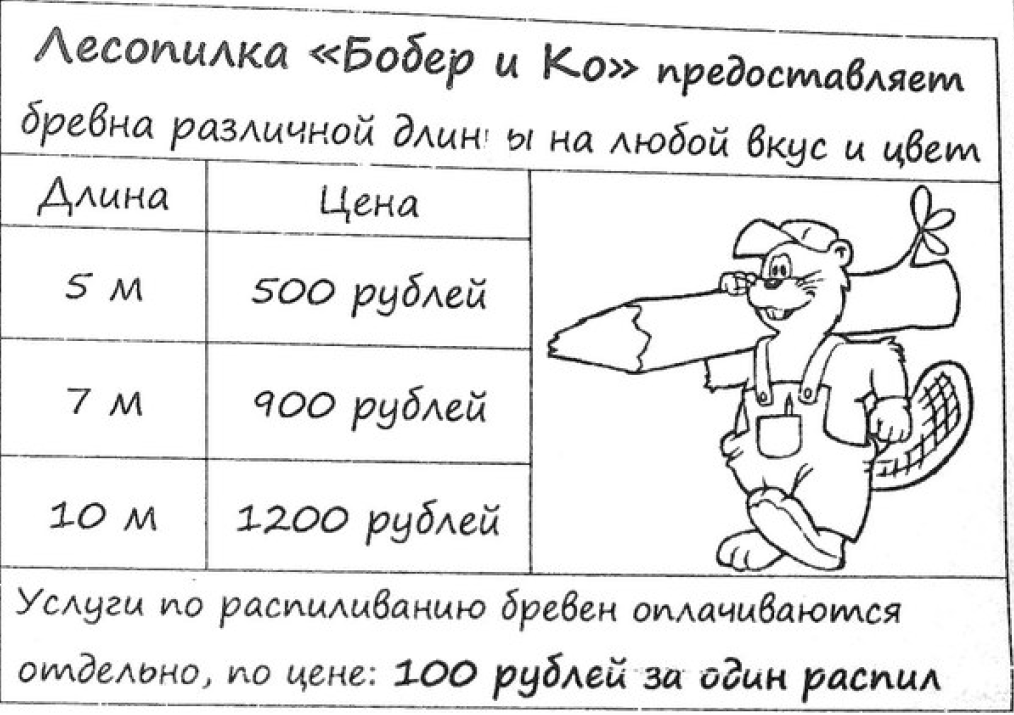
\includegraphics[scale=0.35]{1.png}}
\end{figure}\\
65. Вдоль шоссе стоят три дерева: береза, тополь, дуб. Расстояние между березой и тополем равно 23 м, а между тополем и дубом 47 м. Чему равно расстояние между березой и дубом?\\
66. Вдоль беговой дорожки расставлено 25 флажков на одинаковом расстоянии друг от друга. Вася стартует у первого флажка и бежит с постоянной скоростью. Через 20 секунд он оказывается у 5 флажка. Через какое время Вася добежит до 25 флажка?\\
67. Во сколько раз лестница на 7 этаж дома длиннее, чем лестница на 3 этаж этого же дома?\\
68. В одном ряду 8 камешков на расстоянии 2 см один от другого. В другом --- 15 камешков на расстоянии 1 см один от другого. Какой ряд длиннее?\\
69. Сколько чисел между 485 и  1234?\\
70. Этаж Сони 6 сверху в 25 этажном доме. На каком этаже живет Соня?\\
71. Гарри и Гермиона резали батон волшебной икательной колбасы. Они сделали 5 разрезов. Сколько получилось кусков колбасы?\\
72. Теперь они взяли батон хихикательной колбасы, сделали несколько разрезов и получили 10 кусков. Сколько разрезов они сделали?\\
73. На сей раз наши герои взяли несколько батонов щекотательной колбасы, сделали 8 разрезов и получили 13 кусков. Сколько батонов они взяли?\\
74. Лифт поднимается с первого этажа на третий за 6 секунд. За какое время он поднимется с первого этажа на девятый?\\
75. 12-метровую колбасу распилили на 3-метровые куски за 12 минут. А за сколько времени 12-метровую колбасу можно распилить на 1-метровые куски?\\
76. На каждой перемене Рон съедает по конфете. За неделю (с понедельника по субботу) было 30 уроков. Сколько всего конфет съел Рон?\\
77. Сколько нечётных чисел заключено между 300 и 700?\\
78. Из книги выпал кусок, первая страница которого имеет номер 439, а номер последней записывается теми же цифрами в каком-то другом порядке. Сколько страниц в выпавшем куске?\\
79. Маша испекла на Новый год три торта, для чего ей понадобилось в сумме десять коржей. Между каждыми двумя соседними коржами был намазан сливочный или шоколадный крем. Слоёв сливочного крема было пять. Сколько было слоёв шоколадного крема?\\
80. На глобусе провели 10 меридианов и 11 параллелей. Сколько кусков получилось? (Меридиан --- это дуга от полюса до полюса, параллель --– полный круг.)\\
81. Разрезали листочек на 5 частей, а одну из них --- ещё на 5 частей. Сколько частей получилось?\\
82. На полоске бумаги отмечены вертикальные линии синего, жёлтого и красного цвета. Если разрезать полоску по синим линиям, то получится 5 кусков, если по жёлтым --- 9 кусков, а если по красным --- 11 кусков. Сколько кусков получится, если разрезать полоску по линиям жёлтого и красного цвета?\\
83. Лист бумаги разрезали на три части, затем некоторые из полученных частей также разрезали на 3 части каждую, и так проделали несколько раз. Может ли при подсчёте количества всех частей получиться число 2018, и почему?\\
84. Герда положила в один ряд красные фишки. Затем Кай положил между двумя соседними красными фишками по одной синей. Затем Принц положил между каждыми двумя соседними фишками по две зелёные фишки. Всего получилось 19 фишек. Сколько красных фишек положила Герда?\\
85. Во сколько раз лестница на 4 этаж в школе длиннее лестницы на 2 этаж?\\
86. На каждом километре между городами Лево и Право стоит столб, на котором указано расстояние до обоих городов. Паша посчитал только столбы на которых есть цифра три. Сколько у него получилось столбов, если расстояние между городами 20 км?\\
87. На каждом километре между городами Лево и Право стоит столб, на котором указано расстояние до обоих городов. Паша посчитал только столбы на которых есть цифра пять. Сколько у него получилось столбов, если расстояние между городами 29 км?\\
88. Сколько натуральных чисел от 10 до 110 делится на 2?\\
89. Сколько натуральных чисел от 30 до 330 делится на 3?\\
90. а) Сколько чисел, больших 59 и меньших 1001, делятся на 7?\\
б) Сколько чисел, больших 59 и меньших 1002, делятся на 7?\\
91. а) Сколько чисел, больших 59 и меньших 2002, делятся на 13?\\
б) Сколько чисел, больших 60 и меньших 2003, делятся на 13?\\
92. 29 орехов разложили на несколько тарелок так, что на каждой тарелке хотя бы один орех и на любых двух тарелках разное количество орехов. Какое наибольшее число тарелок могло быть?\\
93. 37 орехов разложили на несколько тарелок так, что на каждой тарелке хотя бы один орех и на любых двух тарелках разное количество орехов. Какое наибольшее число тарелок могло быть?\\
94. Сколько чисел от 1239 до 2200 содержат в своей записи единицу?\\
95. Сколько чисел от 2239 до 3300 содержат двойку в своей записи?\\
96. Интервал между двумя последовательными поездами одинаков и составляет целое число минут. Марк ровно 60 минут смотрел на поезда и насчитал 8 проехавших мимо поездов. Каким может быть интервал движения?\\
97. Интервал между двумя последовательными поездами одинаков и составляет целое число минут. Марк ровно 90 минут смотрел на поезда и насчитал 12 проехавших мимо поездов. Каким может быть интервал движения?\\
98. Бобры Боб и Роб нашли очень длинное бревно для своей плотины. Боб сделал 15 распилов, а Роб распилил каждое получившееся у Боба брёвнышко на 3 части. Сколько в итоге получилось брёвнышек у бобров?\\
99. Сколько существует пятизначных чисел, делящихся на 15?\\
100. Сколько существует пятизначных чисел, делящихся на 21?\\
101. Будем называть число {\it весёлым,} если любые две его соседние цифры имеют разную чётность. Найдите сумму всех весёлых чисел среди данных: 12, 10, 2020206, 123458, 1001.\\
102. Будем называть число {\it грустным,} если любые две его соседние цифры имеют разную чётность. Найдите сумму всех грустных чисел среди данных: 21, 101, 6060602, 123458, 1001.\\
103. В последовательности 3, 4, 7, 1, 8, 9, 7 ... каждая цифра равна последней цифре суммы двух предыдущих цифр. Как видно, на 5-м месте стоит цифра 8. А какая цифра стоит на 2022-м месте?\\
104. В последовательности 9, 2, 1, 3, 4, 7, 1 ... каждая цифра равна последней цифре суммы двух предыдущих цифр. Как видно, на 5-м месте стоит цифра 4. А какая цифра стоит на 2022-м месте?\\
105. Когда Винни-Пух пришёл к Кролику, чтобы немножечко подкрепиться, он заметил, что в кладовой Кролика выше полки с самым вкусным мёдом и ниже неё одинаковое количество полок. Сначала он попробовал варенье, которое стояло тремя полками выше мёда, оттуда спустился на 7 полок вниз, так как там было сгущённое молоко. Так он оказался на 4 полке. Сколько полок в кладовой Кролика?\\
106. Когда кот Матроскин приехал в городскую квартиру Дяди Фёдора, он заметил, что выше этажа, где живёт Дядя Фёдор и ниже его одинаковое количество этажей. Сначала Матроскин случайно поднялся на 4 этажа выше этажа Дяди Фёдора, а потом спустился на 8 этажей вниз, так как забыл там на подоконнике бутерброд. Так он оказался на пятом этаже. Сколько всего этажей в доме, где живёт Дядя Фёдор?\\
107. Олег поставил в тетради точки по прямой линии так, что расстояние между соседними точками равно 3 см. Сколько точек поставил Олег, если расстояние между крайними равно 12 см?\\
108. Аня выше Нади, но ниже Кати. Инна выше Олеси, но ниже Ани. Кто из девочек самая высокая?\\
109. Будем называть число {\it однообразным,} если какие-то две его соседние цифры имеют одинаковую чётность. Найдите сумму всех однообразных чисел среди данных: 101010, 104060, 694936, 1003, 143256.\\
110. Будем называть число {\it однообразным,} если какие-то две его соседние цифры имеют одинаковую чётность. Найдите сумму всех однообразных чисел среди данных: 909090, 504020, 3001, 392978, 652341.\\
111. Сколько существует нечётных чисел, больших 239, но меньших 2339?\\
112. Сколько существует нечётных чисел, больших 239, но меньших 2139?\\
113. Для приготовления бутербродов Антон резал очень длинный батон. Сначала он сделал 11 разрезов, а потом каждый получившийся кусок разрезал ещё на 5 частей. Сколько всего кусков батона получилось?\\
114. Для приготовления бутербродов Алиса резала очень длинный батон. Сначала она сделала 4 разреза, а потом каждый получившийся кусок разрезала ещё на 14 частей. Сколько всего кусков батона получилось?\\
115. 2024 --- год дракона. Черепаха Джонатан родился в 1856 году и жив до сих пор. Сколько раз Джонатан застал год дракона? Год дракона наступает каждые 12 лет.\\
116. 2024 --- год дракона. Черепаха Джонатан родился в 1832 году и жив до сих пор. Сколько раз Джонатан застал год дракона? Год дракона наступает каждые 12 лет.\\
117. Сколько существует нечётных чисел, больших 239 и меньших 777?\\
118. Сколько существует нечётных чисел, больших 329 и меньших 777?\\
119. Трёхзначное число называется {\it красивым,} если его первая цифра чётная, последняя нечётная, а сумма всех трёх цифр равна 7. Сколько красивых чисел?\\
120. Трёхзначное число называется {\it красивым,} если его первая цифра чётная, последняя нечётная, а сумма всех трёх цифр равна 8. Сколько красивых чисел?
\newpage
\section{Раздел 7: Нестандартные задачи}
Большинство задач решаются при помощи теории, изложенной выше.\\
1. Сколько чётных чисел в этом ряду: 16, 27, 258, 2667, 8888?\\
2. Сколько нечётных чисел в этом ряду: 16, 27, 258, 2667, 8888?\\
3. Какое самое маленькое чётное число можно составить из цифр 2, 4, 8 и 9, если каждую цифру надо использовать точно один раз?\\
4. Какое самое большое чётное число можно составить из цифр 2, 4, 8 и 9, если каждую цифру надо использовать точно один раз?\\
5. Расставьте скобки так, чтобы равенство было верным: $7\cdot9+12:3-2=23.$\\
6. Расставьте скобки так, чтобы равенство было верным: $20:2+7\cdot2-5=29.$
\newpage
\noindent7. Разместите числа 1, 2, 3, 4, 5, 6, 7, 8, 9 в пустых кружках так, чтобы сумма трёх чисел расположенных на каждой прямой, была равна 15.
\begin{center}
\begin{figure}[h!]
\center{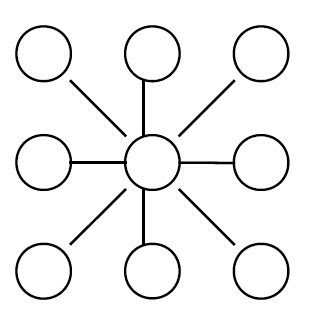
\includegraphics[scale=0.35]{2.png}}
\end{figure}
\end{center}
8. Разместите числа 2, 3, 4, 5, 6, 7, 8, 9, 10 в пустых кружках так, чтобы сумма трёх чисел расположенных на каждой прямой, была равна 18.
\begin{center}
\begin{figure}[h!]
\center{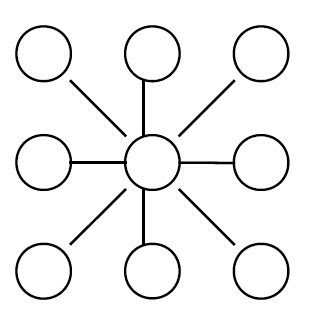
\includegraphics[scale=0.35]{22.png}}
\end{figure}
\end{center}
9. Назовём число {\it хорошим,} если его можно получить, перемножая только двойки и тройки. Перечислите все хорошие числа от 4 до 20.\\
10. Назовём число {\it хорошим,} если его можно получить, перемножая только двойки и пятёрки. Перечислите все хорошие числа от 6 до 30.\\
11. Представьте число 405 в виде произведения нескольких чисел, сумма которых равна 20.\\
12. Представьте число 575 в виде произведения нескольких чисел, сумма которых равна 37.\\
13. Имеются два кувшина: один объёмом 8 л, а второй --- объёмом 5 или 6 литров. На взгляд нельзя определить объём кувшина или воды в нём. Опишите, как определить объём второго кувшина, находясь возле реки.\\
14. Имеются два кувшина: один объёмом 5 л, а второй --- объёмом 3 или 4 литров. На взгляд нельзя определить объём кувшина или воды в нём. Опишите, как определить объём второго кувшина, находясь возле реки.\\
15. В шахматном турнире участвуют 14 человек. Сколько партий будет сыграно в турнире, если каждый участник сыграет со всеми остальными участниками по одному разу?\\
16. В чемпионате России по футболу участвуют 16 команд. Сколько матчей будет сыграно в чемпионате, если каждая команда сыграет со всеми остальными командами дважды?\\
17. Расположите в кружочках числа от 1 до 10 так, чтобы для любых двух соседних чисел их сумма была равна сумме двух чисел, им противоположных (симметричных относительно центра окружности).
\begin{center}
\begin{figure}[ht!]
\center{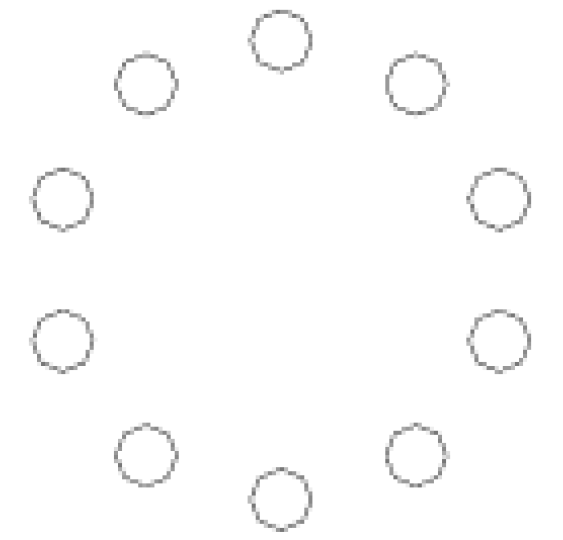
\includegraphics[scale=0.35]{3.png}}
\end{figure}
\end{center}
\newpage
\noindent18. Расположите в кружочках числа от 11 до 20 так, чтобы для любых двух соседних чисел их сумма была равна сумме двух чисел, им противоположных (симметричных относительно центра окружности).
\begin{center}
\begin{figure}[ht!]
\center{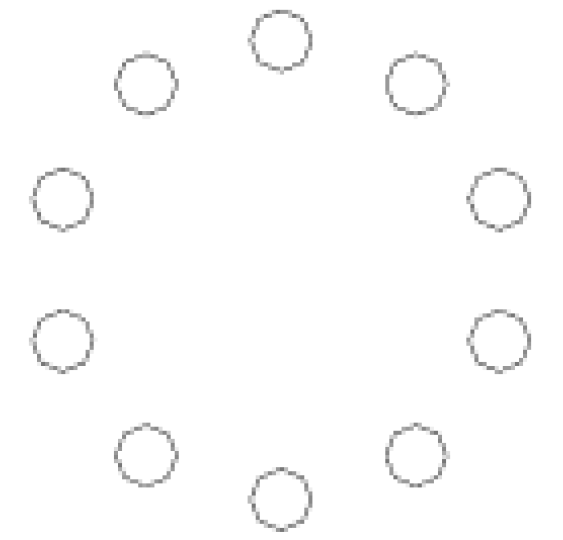
\includegraphics[scale=0.35]{33.png}}
\end{figure}
\end{center}
19. Сколько квадратов изображено на рисунке (все стороны маленьких квадратиков одинаковы)?
\begin{center}
\begin{figure}[ht!]
\center{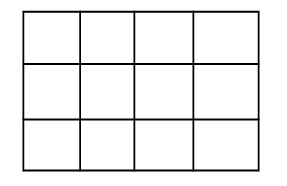
\includegraphics[scale=0.35]{4.png}}
\end{figure}
\end{center}
20. Сколько квадратов изображено на рисунке (все стороны маленьких квадратиков одинаковы)?
\begin{center}
\begin{figure}[ht!]
\center{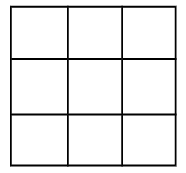
\includegraphics[scale=0.35]{44.png}}
\end{figure}
\end{center}
21. Сколько существует трёхзначных чисел, у которых все цифры чётные?\\
22. Сколько существует чётных трёхзначных чисел?\\
23. Какова разность между наибольшим и наименьшим четырёхзначными числами, все цифры которых различны?\\
24. Какова сумма наибольшего и наименьшего четырёхзначных чисел, все цифры которых различны?\\
25. Встретились три друга: Белов, Чернов и Рыжов. Один из них блондин, другой брюнет, а третий рыжий. Брюнет сказал Белову: <<Ни у кого из нас цвет волос не соответствует фамилии>>. Какой цвет волос у каждого из них?\\
26. В лесу проводился кросс. Белка сказала: <<Первое место занял заяц, а второй была лиса>>. Другая белка возразила: <<Заяц занял второе место, а лось был первым>>. На что филин заметил, что в высказывании каждой белки одна часть верная, а другая нет. Кто был первым, а кто вторым в кроссе?\\
27. Расставьте между цифрами знаки действий и скобки так, чтобы получилось верное равенство:\\ 5 4 3 2 1 = 100.\\
28. Расставьте между цифрами знаки действий и скобки так, чтобы получилось верное равенство:\\ 6 8 20 4 2 = 58.\\
29. Петя ходит в бассейн один раз в два дня, Коля --- один раз в 4 дня, а Вова --- один раз в пять дней. Они встретились в бассейне во вторник. В какой день недели они встретятся вновь?\\
30. Марина ходит в спортзал один раз в 6 дней, Маша --- один раз в 3 дня, а Катя --- один раз в 4 дня. Они встретились в спортзале в субботу. В какой день недели они встретятся вновь?
\newpage
\noindent31. Расставьте в клетках данной таблицы числа 4, 5, 6, 7, 8, 9, 10, 11, 12 (по одному каждое) так, чтобы сумма чисел в каждой строке, каждом столбце и на двух главных диагоналях была равна 24.
\begin{center}
\begin{figure}[ht!]
\center{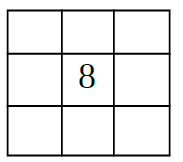
\includegraphics[scale=0.35]{5.png}}
\end{figure}
\end{center}
32. Расставьте в клетках данной таблицы числа 0, 1, 2, 3, 4, 5, 6, 7, 8 (по одному каждое) так, чтобы сумма чисел в каждой строке, каждом столбце и на двух главных диагоналях была одинаковой.
\begin{center}
\begin{figure}[ht!]
\center{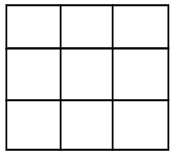
\includegraphics[scale=0.35]{55.png}}
\end{figure}
\end{center}
33. На какую цифру оканчивается сумма $9\times19\times29\times\ldots\times20129+1?$\\
34. На какую цифру оканчивается разность $4\times14\times24\times\ldots\times20124-1?$\\
35. Сколько существует пятизначных чисел, у которых третья цифра 7, а последняя цифра чётная?\\
36. Сколько различных трёхзначных чисел, меньших 400, можно составить из цифр 1, 3, 5, 7, 9, если любая из этих цифр может быть использована только один раз?\\
37. В числе 3728106 зачеркните 3 цифры так, чтобы оставшиеся цифры (в той же последовательности) образовывали:\\
а) возможно большее четырёхзначное число;\\
б) возможно меньшее четырёхзначное число.\\
38. В числе 4791402 зачеркните 3 цифры так, чтобы оставшиеся цифры (в той же последовательности) образовывали:\\
а) возможно большее четырёхзначное число;\\
б) возможно меньшее четырёхзначное число.\\
39. Сколькими способами можно расставить на полке томики стихов Пушкина, Лермонтова, Некрасова, Маршака и Барто, чтобы Пушкин стоял на первом месте, а Маршак и Барто стояли рядом?\\
40. Сколькими способами можно расставить на полке томики сказок Пушкина, Андерсена, Перро, Бажова и Гримм, чтобы Пушкин стоял на первом месте, а Бажов и Андерсен стояли рядом?\\
41. Перед вами МНОГОУГОЛЬНИК. У него может быть сколько угодно ВЕРШИН. ({\it На предложенном рисунке их всего 6, для примера.}) Представьте себе двадцатиугольник (у него 20 вершин). Одну из его вершин соединим отрезками со всеми остальными. На сколько треугольников мы разделим двадцатиугольник?
\begin{center}
\begin{figure}[ht!]
\center{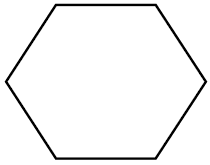
\includegraphics[scale=0.35]{6.png}}
\end{figure}
\end{center}
42. Перед вами МНОГОУГОЛЬНИК. У него может быть сколько угодно ВЕРШИН. ({\it На предложенном рисунке их всего 6, для примера.}) Представьте себе тридцатиугольник (у него 30 вершин). Одну из его вершин соединим отрезками со всеми остальными. На сколько треугольников мы разделим тридцатиугольник?
\begin{center}
\begin{figure}[ht!]
\center{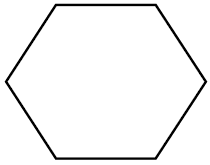
\includegraphics[scale=0.35]{6.png}}
\end{figure}
\end{center}
\newpage
\noindent43. В клетках квадрата $3\times3$ были записаны натуральные числа так, что суммы в каждой строке, в каждом столбце и на каждой диагонали были одинаковыми. Некоторые числа стёрли. Восстановите стёртые числа.
\begin{center}
\begin{figure}[ht!]
\center{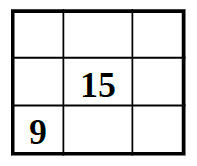
\includegraphics[scale=0.35]{7.png}}
\end{figure}
\end{center}
44. В клетках квадрата $3\times3$ были записаны натуральные числа так, что суммы в каждой строке, в каждом столбце и на каждой диагонали были одинаковыми. Некоторые числа стёрли. Восстановите стёртые числа.
\begin{center}
\begin{figure}[ht!]
\center{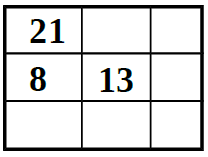
\includegraphics[scale=0.35]{77.png}}
\end{figure}
\end{center}
45. Расставьте четыре нечётных числа, среди которых нет равных, в квадраты так, чтобы их сумма равнялась 50.
\begin{center}
\begin{figure}[ht!]
\center{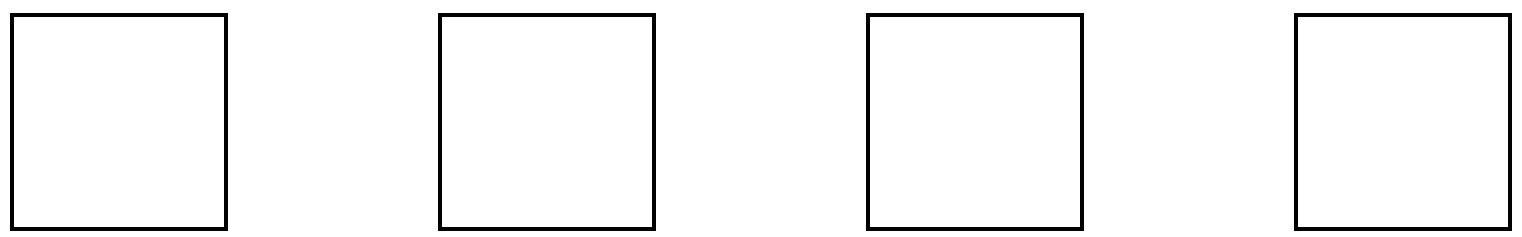
\includegraphics[scale=0.35]{8.png}}
\end{figure}
\end{center}
46. Расставьте четыре нечётных числа, среди которых нет равных, в квадраты так, чтобы их сумма равнялась 56.
\begin{center}
\begin{figure}[ht!]
\center{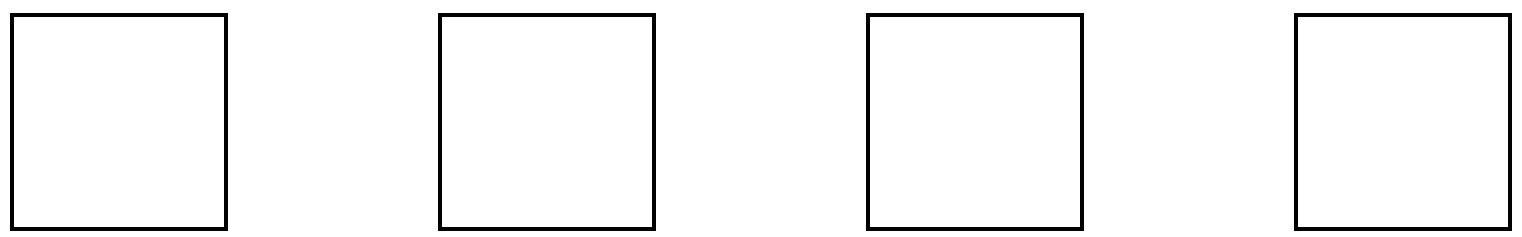
\includegraphics[scale=0.35]{8.png}}
\end{figure}
\end{center}
47. Придумайте пять различных чисел с суммой 120 таких, что любые два из них отличаются не более, чем на 4. В ответ запишите пять чисел через запятую.\\
48. Придумайте пять различных чисел с суммой 110 таких, что любые два из них отличаются не более, чем на 4. В ответ запишите пять чисел через запятую.\\
49. Сколько существует стозначных чисел, сумма цифр которых равна 16, у которых в разряде десятков стоит 2, в разряде сотен --- 3, а в разряде миллиардов --- 9?\\
50. Сколько существует девяностозначных чисел, сумма цифр которых равна 17, у которых в разряде сотен стоит 2, в разряде тысяч --- 4, а в разряде миллионов --- 9?\\
51. На рисунке изображена буква {\bf Т} ширины 7, высоты 6, а толщина ножки и шляпки у неё 3 клетки. Сколько клеток содержит аналогичная буква {\bf Т} ширины 70, высоты 60 и толщиной ножки и шляпки 6 клеток?
\begin{center}
\begin{figure}[ht!]
\center{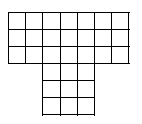
\includegraphics[scale=0.35]{9.png}}
\end{figure}
\end{center}
\newpage
\noindent52. На рисунке изображена буква {\bf Т} ширины 7, высоты 6, а толщина ножки и шляпки у неё 3 клетки. Сколько клеток содержит аналогичная буква {\bf Т} ширины 60, высоты 70 и толщиной ножки и шляпки 8 клеток?
\begin{center}
\begin{figure}[ht!]
\center{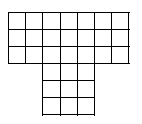
\includegraphics[scale=0.35]{9.png}}
\end{figure}
\end{center}
53. На рисунке изображена буква {\bf П} ширины 7, высоты 5, а толщина ножек и перекладины у неё 2 клетки. Сколько клеток содержит аналогичная буква {\bf П} ширины 70, высоты 60 и с толщиной ножки и перекладины 6 клеток?
\begin{center}
\begin{figure}[ht!]
\center{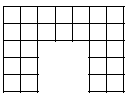
\includegraphics[scale=0.35]{10.png}}
\end{figure}
\end{center}
54. На рисунке изображена буква {\bf П} ширины 7, высоты 5, а толщина ножек и перекладины у неё 2 клетки. Сколько клеток содержит аналогичная буква {\bf П} ширины 60, высоты 80 и с толщиной ножки и перекладины 7 клеток?
\begin{center}
\begin{figure}[ht!]
\center{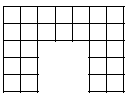
\includegraphics[scale=0.35]{10.png}}
\end{figure}
\end{center}
55. Придумайте пять различных двузначных нечётных чисел с суммой 375. В ответ запишите пять чисел через запятую.\\
56. Придумайте пять различных двузначных нечётных чисел с суммой 115. В ответ запишите пять чисел через запятую.\\
57. Расставьте цифры от 1 до 9 (каждую по одному разу) в квадратики так, чтобы все равенства были верными.
\begin{center}
\begin{figure}[ht!]
\center{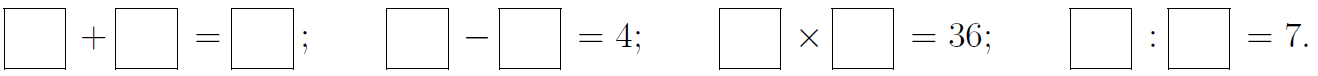
\includegraphics[scale=0.35]{11.png}}
\end{figure}
\end{center}
58. Расставьте цифры от 1 до 9 (каждую по одному разу) в квадратики так, чтобы все равенства были верными.
\begin{center}
\begin{figure}[ht!]
\center{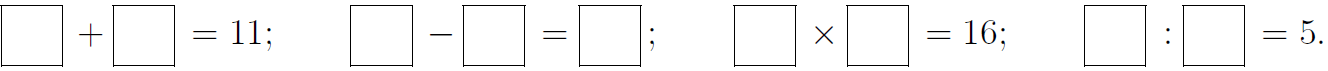
\includegraphics[scale=0.35]{111.png}}
\end{figure}
\end{center}
59. Сколько есть способов вычеркнуть несколько цифр из числа 56115664783047830888 так, чтобы осталось число 478?\\
60. Сколько есть способов вычеркнуть несколько цифр из числа 32111235692056920999 так, чтобы осталось число 569?\\
61. Суммарная длина перегородок в клетчатом прямоугольнике $4\times5$ на рисунке равна 31. Чему равна суммарная длина перегородок в прямоугольнике $12\times50?$
\begin{center}
\begin{figure}[ht!]
\center{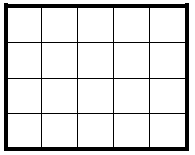
\includegraphics[scale=0.35]{12.png}}
\end{figure}
\end{center}
\newpage
\noindent62. Суммарная длина перегородок в клетчатом прямоугольнике $4\times5$ на рисунке равна 31. Чему равна суммарная длина перегородок в прямоугольнике $40\times15?$
\begin{center}
\begin{figure}[ht!]
\center{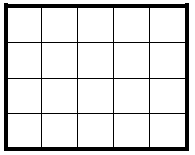
\includegraphics[scale=0.35]{12.png}}
\end{figure}
\end{center}
63. Придумайте шесть различных чисел, которые отличаются только последней цифрой, а их сумма равна 2017. В ответ запишите их через запятую.\\
64. Придумайте шесть различных чисел, которые отличаются только последней цифрой, а их сумма равна 2057. В ответ запишите их через запятую.\\
65. Брат мужа называется {\it деверь,} сестра мужа называется {\it золовка,} мать мужа называется {\it свекровь,} отец мужа называется {\it свёкр,} отец жены называется {\it тесть,} мать жены называется {\it тёща,} брат жены называется {\it шурин,} сестра жены называется {\it свояченица.} Александр женился на Марии, и у них родились дети: Ксения, Георгий, Михаил, Ольга. Сестра Марии Александра вышла замуж за Эдуарда, у них родился сын Виктор. Михаил женился на Наталье, Ксения вышла замуж за Николая, у них родились Фёдор и Никита. Ольга вышла замуж за Петра. Как зовут сына свояченицы отца деверя Натальи?\\
66.  Брат мужа называется {\it деверь,} сестра мужа называется {\it золовка,} мать мужа называется {\it свекровь,} отец мужа называется {\it свёкр,} отец жены называется {\it тесть,} мать жены называется {\it тёща,} брат жены называется {\it шурин,} сестра жены называется {\it свояченица.} Иван женился на Марии, и у них родились дети: Александр, Евгения, Максим, Ольга. Сестра Марии Александра вышла замуж за Павла, у них родился сын Василий. Максим женился на Анне, Евгения вышла замуж за Дмитрия, у них родились Фёдор и Никита. Ольга вышла замуж за Петра. Как зовут сына свояченицы отца деверя Анны?\\
67. Нарисуйте фигуру, состоящую из десяти клеток $1\times1,$ периметр которой равен 18.\\
68. Нарисуйте фигуру, состоящую из девяти клеток $1\times1,$ периметр которой равен 16.\\
69. Один литр --- это кубический дециметр. На уроке труда Вася сделал стальную заготовку для ванны с прямоугольным основанием, изображённую на схеме (пунктирные линии обозначают места сгиба). Сторона одной клеточки равна 1 дециметру. Сварив края ванны, Вася обнаружил, что она вышла кривая. Какое наибольшее количество литров воды войдёт в ванну?
\begin{center}
\begin{figure}[ht!]
\center{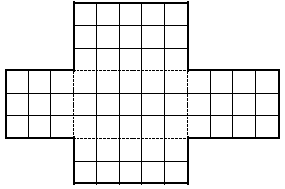
\includegraphics[scale=0.35]{13.png}}
\end{figure}
\end{center}
70. Один литр --- это кубический дециметр. На уроке труда Вася сделал стальную заготовку для ванны с прямоугольным основанием, изображённую на схеме (пунктирные линии обозначают места сгиба). Сторона одной клеточки равна 1 дециметру. Сварив края ванны, Вася обнаружил, что она вышла кривая. Какое наибольшее количество литров воды войдёт в ванну?
\begin{center}
\begin{figure}[ht!]
\center{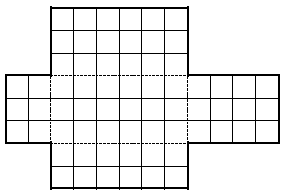
\includegraphics[scale=0.35]{133.png}}
\end{figure}
\end{center}
\newpage
\noindent
71. На рисунке изображена буква О ширины 5, высоты 7, толщины 2 клетки. Суммарная длина её внутренних перегородок равна 48. Чему равна суммарная длина внутренних перегородок буквы О, у которой толщина 4, высота 40, ширина 30 клеток?
\begin{center}
\begin{figure}[ht!]
\center{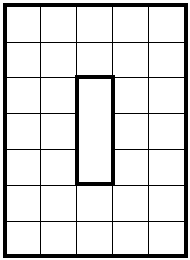
\includegraphics[scale=0.35]{14.png}}
\end{figure}
\end{center}
72. На рисунке изображена буква О ширины 5, высоты 7, толщины 2 клетки. Суммарная длина её внутренних перегородок равна 48. Чему равна суммарная длина внутренних перегородок буквы О, у которой толщина 4, высота 30, ширина 20 клеток?
\begin{center}
\begin{figure}[ht!]
\center{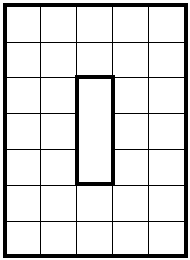
\includegraphics[scale=0.35]{14.png}}
\end{figure}
\end{center}
73. В большую квадратную комнату внесли два квадратных ковра. Сторона одного из ковров в два раза больше стороны другого. Оказалось, что если положить ковры в противоположные углы комнаты, то они покроют в два слоя участок пола площадью $4\text{м}^2.$ А если положить ковры в соседние углы комнаты, то в два слоя окажется покрыт участок площадью $14\text{м}^2.$ Чему равна сторона комнаты?\\
74. В большую квадратную комнату внесли два квадратных ковра. Сторона одного из ковров в два раза больше стороны другого. Оказалось, что если положить ковры в противоположные углы комнаты, то они покроют в два слоя участок пола площадью $9\text{м}^2.$ А если положить ковры в соседние углы комнаты, то в два слоя окажется покрыт участок площадью $15\text{м}^2.$ Чему равна сторона комнаты?\\
75. Сумма двух чисел равна 8481. Одно из них оканчивается нулём. Если этот нуль зачеркнуть, то получится второе число. Найдите эти числа.\\
76. Будем говорить, что прямоугольника имеет пузатость $2:1,$ если одна его сторона в два раза больше другой. А у прямоугольника со сторонами 3см и 2см пузатость равна $3:2.$ Было два прямоугольника, у каждого из которых пузатость равнялась $4:1.$ Из них сложили один прямоугольник. Чему может быть равна его пузатость?\\
77. Будем говорить, что прямоугольника имеет пузатость $2:1,$ если одна его сторона в два раза больше другой. А у прямоугольника со сторонами 3см и 2см пузатость равна $3:2.$ Было два прямоугольника, у каждого из которых пузатость равнялась $3:1.$ Из них сложили один прямоугольник. Чему может быть равна его пузатость?\\
78. Сколько существует таких натуральных чисел $N,$ для которых {\bf ровно одно} из чисел $N$ и $N+937$ трёхзначное?\\
79. Сколько существует таких натуральных чисел $N,$ для которых {\bf ровно одно} из чисел $N$ и $N+973$ трёхзначное?\\
80. Сколько существует чётных пятизначных чисел с произведением цифр 20?\\
81. Сколько существует чётных пятизначных чисел с произведением цифр 28?\\
82. На электронных часах высвечивается 13:00:07. Через какое время впервые все цифры на табло часов окажутся разными?\\
83. На электронных часах высвечивается 12:00:08. Через какое время впервые все цифры на табло часов окажутся разными?\\
84. В трёх пассажирских поездах различное число мест: 236, 295, 472. Во всех вагонах число мест одинаковое и большее 30. Сколько вагонов в этих поездах вместе?\\
85. В трёх пассажирских поездах различное число мест: 265, 318, 477. Во всех вагонах число мест одинаковое и большее 30. Сколько вагонов в этих поездах вместе?\\
86. На рисунке изображены две клетчатые фигуры: прямоугольник $7\times8$ с дыркой и буква $L$ странной формы. У каждой из фигур одна клетка отмечена чёрным. Эти фигуры по клеточкам положили на тетрадный лист так, что чёрные клетки находятся в точности друг над другом. Клетки фигуры и клетки листа совпадают. Фигурки можно поворачивать и переворачивать. Алина посчитала, сколько клеток тетрадного листа накрыто хотя бы одной из фигурок. Какие числа она могла получить? В ответ запишите {\bf все возможные} варианты через запятую.
\begin{center}
\begin{figure}[ht!]
\center{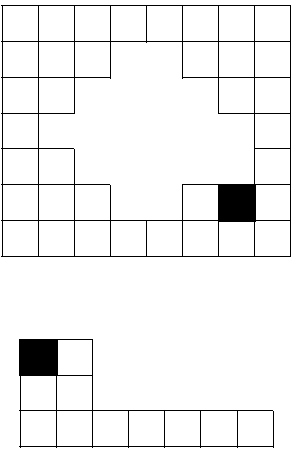
\includegraphics[scale=0.35]{15.png}}
\end{figure}
\end{center}
87. На рисунке изображены две клетчатые фигуры: прямоугольник $7\times9$ с дыркой и буква $P$ странной формы. У каждой из фигур одна клетка отмечена чёрным. Эти фигуры по клеточкам положили на тетрадный лист так, что чёрные клетки находятся в точности друг над другом. Клетки фигуры и клетки листа совпадают. Фигурки можно поворачивать и переворачивать. Алина посчитала, сколько клеток тетрадного листа накрыто хотя бы одной из фигурок. Какие числа она могла получить? В ответ запишите {\bf все возможные} варианты через запятую.
\begin{center}
\begin{figure}[ht!]
\center{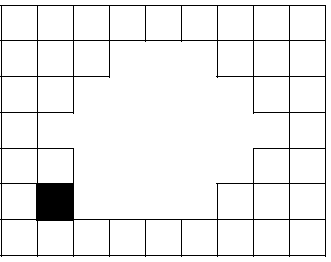
\includegraphics[scale=0.35]{155.png}}
\center{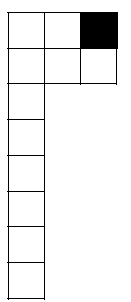
\includegraphics[scale=0.35]{156.png}}
\end{figure}
\end{center}
88. Миша выбирает какие-нибудь три года из XXI века, перемножает цифры каждого года и складывает полученные произведения. Какое самое большое число он может получить?\\
89. Зоя выбирает какие-нибудь три года из XXI века, перемножает цифры каждого года и складывает полученные произведения. Какое самое большое число она может получить?\\
90. Некоторые из городов A, B, C, D и E соединены между собой дорогами. Любые два города соединены не более, чем одной дорогой (может и не быть дороги, ведущей напрямую из одного города в другой). Из города A выходят 4 дороги, из городов B и E по 2 дороги, из городов C и D по 3 дороги. Из следующих утверждений выберите ровно одно верное:\\
А) Из города A нельзя напрямую попасть в город D;\\
Б) Из города B нельзя напрямую попасть в город E;\\
В) Из города D можно напрямую попасть и в город B, и в город E.\\
Г) Из города C можно напрямую попасть либо в город А, либо в город D.\\
91. Некоторые из городов К, Л, М, Н и О соединены между собой дорогами. Любые два города соединены не более, чем одной дорогой (может и не быть дороги, ведущей напрямую из одного города в другой). Из города О выходят 4 дороги, из городов К и Л по 2 дороги, из городов М и Н по 3 дороги. Из следующих утверждений выберите ровно одно верное:\\
А) Из города О нельзя напрямую попасть в город Л;\\
Б) Из города Л нельзя напрямую попасть в город К;\\
В) Из города Н можно напрямую попасть и в город К, и в город Л.\\
Г) Из города М можно напрямую попасть либо в город Н, либо в город О.\\
92. Шерлок Холмс получил записку, в которой сказано: {\it <<Барон М. солгал, когда сказал, что неправда, что А и Б одновременно сидели на трубе.>>} В этой записке написана ложь. Это означает, что:\\
А) А и Б одновременно сидели на трубе;\\
Б) На трубе обязательно сидел только Б;\\
В) А и Б не сидели на трубе одновременно;\\
Г) Б совершенно точно не сидел на трубе.\\
93. Доктор Ватсон получил записку, в которой сказано: {\it <<Кучер обманул Вас, когда сказал, что неправда, что А и Б одновременно НЕ сидели на трубе.>>} В этой записке написана ложь. Это означает, что:\\
А) А и Б одновременно сидели на трубе;\\
Б) На трубе обязательно сидел только Б;\\
В) А и Б не сидели на трубе одновременно;\\
Г) Б совершенно точно не сидел на трубе.\\
94. Крокодил Гена разложил по четырём коробкам нужные вещи. В одной коробке у него лежали лампочки, в другой гвозди, в третьей нитки и иголки, в четвёртой нитки и лампочки. Для коробок он приготовил этикетки: Л, Г, НИ, НЛ. Пока он отвернулся, Шапокляк приклеила этикетки так, что ничего из упомянутого на этикетке не находится в коробке, на которую она наклеена. Что лежит в коробке с этикеткой Л?\\
95. Знайка разложил по четырём коробкам нужные вещи. В одной коробке у него лежали шапочки, в другой тапочки, в третьей книжки и блокноты, в четвёртой книжки и шапочки. Для коробок он приготовил этикетки: Ш, Т, КБ, КШ. Пока он отвернулся, Незнайка приклеил этикетки так, что ничего из упомянутого на этикетке не находится в коробке, на которую она наклеена. Что лежит в коробке с этикеткой Т?\\
96. Найдите наименьшее трёхзначное число, которое делится на 3, и первая цифра которого равна 4.\\
97. В коробке лежат 100 синих и 100 красных шаров. Какое наименьшее число шаров надо вытащить, не заглядывая в коробку, чтобы среди них наверняка было 5 шаров одного цвета?\\
98. Какие четыре цифры надо вычеркнуть из числа 5837609, чтобы получившееся трёхзначное число было как можно меньше?\\
99. Из чисел 2, 3, 8, 18, 92, 238, 568 выберите делимое, делитель, частное и остаток.\\
100. Используя только цифры 0, 2, 3, 4 запишите такое наименьшее шестизначное число, чтобы каждая из цифр 0, 2, 3, 4 в нём присутствовала.\\
101. На рисунке изображена развёртка игрального кубика. Сумма цифр на любых двух противоположных гранях равна 7. Какой может быть наибольшая разность цифр на закрашенных гранях? Напоминаем, что на всех гранях стоят разные цифры от 1 до 6.
\begin{center}
\begin{figure}[ht!]
\center{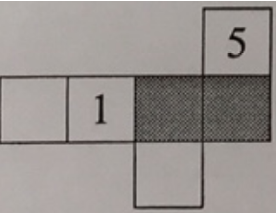
\includegraphics[scale=0.35]{17.png}}
\end{figure}
\end{center}
102. У Саши 20 кубиков, у Васи 27 кубиков, у Вани 18 кубиков, а у Олега --- 10 кубиков. Кто из мальчиков может построить куб из всех своих кубиков?\\
103. На пикник отправились пятеро мужчин из одной семьи: дедушка, два его сына и два внука. Их зовут: Олег Игоревич, Николай Олегович, Игорь Николаевич, Василий Александрович и Александр Игоревич. Какое имя у дедушки?\newpage
\noindent104. На рисунке изображена развёртка игрального кубика. Сумма цифр на любых двух противоположных гранях равна 7. Какой может быть наибольшая разность цифр на закрашенных гранях? Напоминаем, что на всех гранях стоят разные цифры от 1 до 6.
\begin{center}
\begin{figure}[ht!]
\center{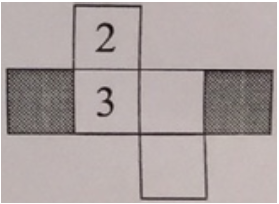
\includegraphics[scale=0.35]{177.png}}
\end{figure}
\end{center}
105. На рисунке изображены несколько верёвок. На каких из них завяжется узел, если потянуть их за концы?
\begin{center}
\begin{figure}[ht!]
\center{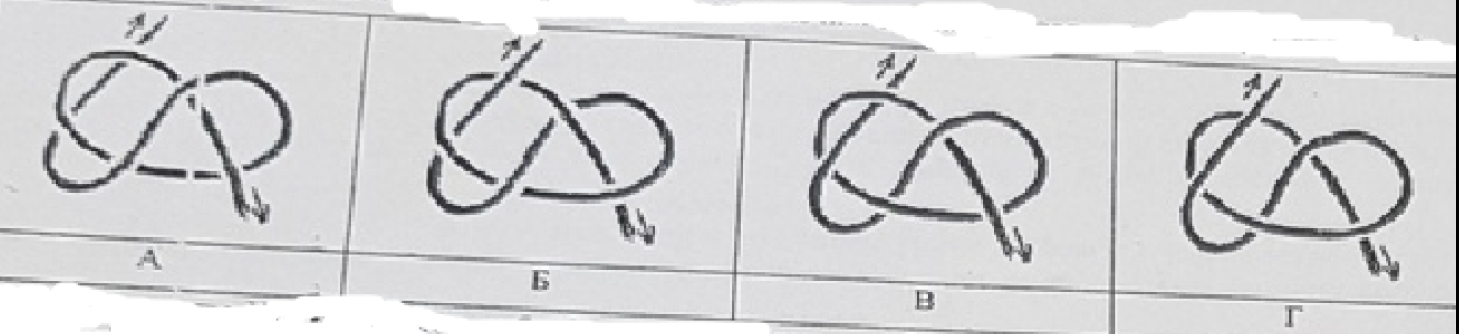
\includegraphics[scale=0.35]{18.png}}
\end{figure}
\end{center}
106. На рисунке изображены несколько верёвок. На каких из них завяжется узел, если потянуть их за концы?
\begin{center}
\begin{figure}[ht!]
\center{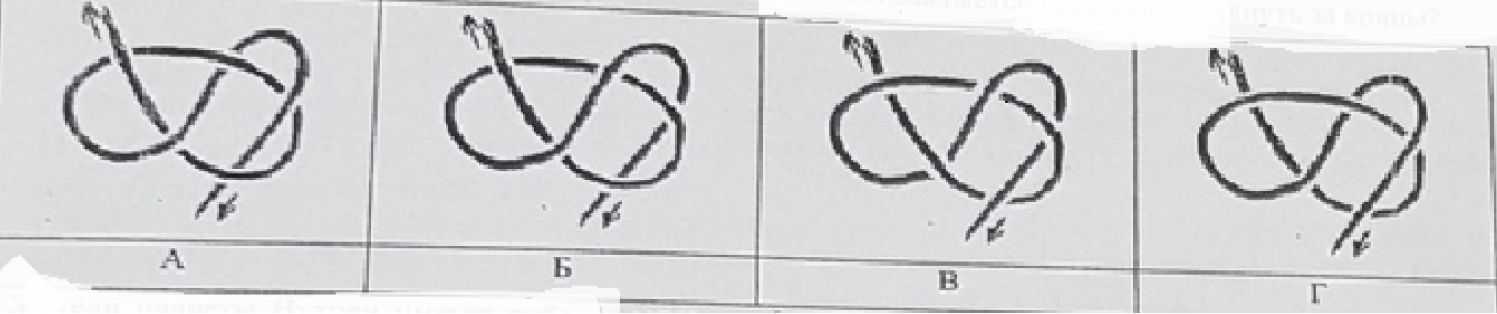
\includegraphics[scale=0.35]{188.png}}
\end{figure}
\end{center}
107. Соловей-разбойник, попав в темницу, рассказывал, что в схватке ему удалось победить Алёшу Поповича, или Добрыню Никитича, или даже обоих. При этом Соловей-разбойник как обычно врал. Как же обстояли дела на самом деле? Выберите {\it все} возможные варианты произошедшего.\\
А) Возможно, Соловья-разбойника пленил Илья Муромец;\\
Б) Возможно, Соловей-разбойник победил Алёшу, но не Добрыню;\\
В) Возможно, Соловей-разбойник победил Добрыню, но не Алёшу;\\
Г) Ни Добрыня, ни алёша не были побеждены Соловьём-разбойником.\\
108. Баба Яга рассказывала, что на конкурсе красоты она победила Василису Прекрасную, или Василису Премудрую, или даже обеих. При этом Баба Яга как обычно врала. Как же обстояли дела на самом деле? Выберите {\it все} возможные варианты произошедшего.\\
А) Возможно, Баба Яга победила Василису Прекрасную, но не Василису Премудрую;\\
Б) Возможно, Баба Яга победила Василису Премудрую, но не Василису Прекрасную;\\
В) Ни одна Василиса не была побеждена Бабой Ягой;\\
Г) Возможно, Баба Яга победила Кикимору Болотную.\\
109. Оля отправила по почте 2 письма Зое. Изначально у Оли было 6 марок, которые стоили 18 рублей, 21 рубль, 24 рубля, 27 рублей, 30 рублей и 33 рубля. После отправки у Оли осталась одна марка. Какая марка осталась, если письма стоили одинаково?\\
110. Алёша отправил по почте 2 письма Олегу. Изначально у Алёши было 6 марок, которые стоили 20 рублей, 24 рубля, 28 рублей, 32 рубля, 36 рублей и 40 рублей. После отправки у Алёши осталась одна марка. Какая марка могла остаться, если письма стоили одинаково?
\newpage
\noindent111. Из одинаковых кубиков склеена фигура. Её сфотографировали спереди, сверху и справа. Каким может быть максимальное количество кубиков в этой фигуре?
\begin{center}
\begin{figure}[ht!]
\center{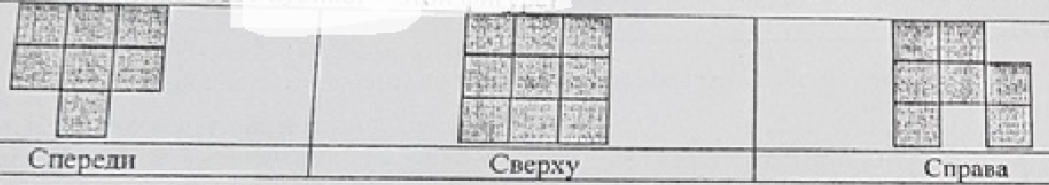
\includegraphics[scale=0.35]{19.png}}
\end{figure}
\end{center}
112. Из одинаковых кубиков склеена фигура. Её сфотографировали спереди, сверху и слева. Каким может быть максимальное количество кубиков в этой фигуре?
\begin{center}
\begin{figure}[ht!]
\center{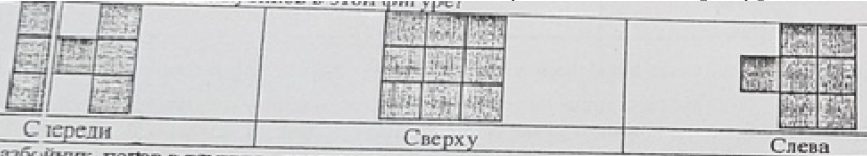
\includegraphics[scale=0.35]{199.png}}
\end{figure}
\end{center}
113. Запишите четырёхзначное число, в котором число десятков вдвое меньше, чем число тысяч; если число сотен умножить на число тысяч, то число сотен не изменится; число единиц на 7 больше числа тысяч.\\
114. Запишите четырёхзначное число, в котором число сотен втрое меньше, чем число тысяч; если число десятков умножить на число тысяч, то число десятков не изменится; число единиц на 5 больше числа тысяч.\\
115. Нарисуйте недостающие фигурки в пустых клетках.
\begin{center}
\begin{figure}[ht!]
\center{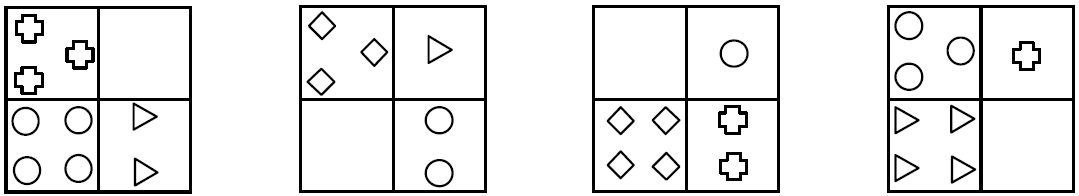
\includegraphics[scale=0.35]{20.png}}
\end{figure}
\end{center}
116. Фукс пообещал капитану Врунгелю, что выучит испанский язык или побывает на полюсе. Пока Фукс не выполнил своё обещание. Это означает, что он\\
а) выучил испанский язык, но пока не был на полюсе;\\
б) не выучил испанский язык и на полюсе пока не был;\\
в) побывал а полюсе, но испанский пока не выучил;\\
г) выучил испанский и побывал на полюсе.\\
117. На рисунке изображена развёртка куба. Рядом изображён куб, собранный из этой же развёртки. Сколько точек на той грани, которой этот куб стоит на столе?
\begin{center}
\begin{figure}[ht!]
\center{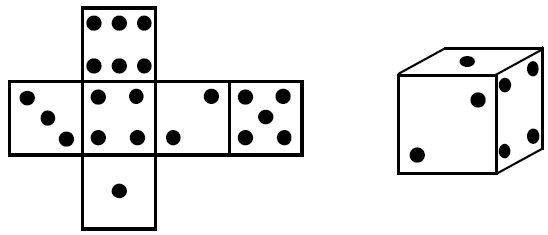
\includegraphics[scale=0.35]{21.png}}
\end{figure}
\end{center}
118. Муравьишка ползает по клетчатому полю $5\times5$ клеток. Он начинает свой путь в правой верхней клетке. Оттуда он ползёт на 2 клетки влево, потом на 4 клетки вниз, потом на 1 клетку вправо, потом на 2 клетки вверх, потом на 3 клетки влево, потом на 1 клетку вверх, потом на 4 клетки вправо, потом на 2 клетки вниз, потом на 3 клетки влево, потом на 2 клетки вверх, потом на 1 клетку вправо, потом на 1 клетку вверх, и оттуда на 2 клетки вправо. Муравьишка не перепрыгивает через клетки на своём пути. В скольких клетках Муравьишка не побывал за время своего путешествия?\\
119. Электронное табло сделано из ламп, как показано на рисунке. На табло меняются числа от 00 до 99. Например, на рисунке показано число 72. Сколько раз в одной из цифр будет гореть на 2 лампы больше, чем в другой?
\begin{center}
\begin{figure}[ht!]
\center{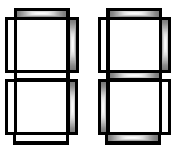
\includegraphics[scale=0.35]{222.png}}
\end{figure}
\end{center}
120. Вася построил большой куб из кубиков. Потом он убрал часть кубиков из всех слоёв, кроме нижнего. Теперь каждый слой кубиков имеет форму квадрата, а сбоку конструкция выглядит так, как на рисунке. сколько кубиков убрал Вася?
\begin{center}
\begin{figure}[ht!]
\center{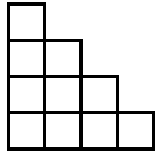
\includegraphics[scale=0.35]{333.png}}
\end{figure}
\end{center}
121. Нарисуйте на клетчатой бумаге какой-нибудь десятиугольник с площадью десять с половиной $\text{см}^2.$ Сторона клетки --- половина сантиметра.\\
122. Садовник Порфирий решил посадить вишнёвый сад на участке длиной 200 м, шириной 100 м. Для этого весь участок он разделил на квадраты $10\times10$ м. В центр каждого такого квадрата и в место, где соединяются границы четырёх квадратов, он посадил саженец вишни. Сколько саженцев понадобилось Порфирию?\\
123. В магазине продавали футболки, кепки и шорты: красные и синие. К концу рабочего дня много товара продали, и оказалось, что все оставшиеся кепки синие, а из красных вещей остались только футболки. Какие из утверждений наверняка верны (их может быть несколько или не быть совсем)? К концу рабочего дня: 1) Нет красных кепок. 2) Все футболки красные. 3) Все кроссовки зелёные. 4) Все шорты синие. 5) Некоторые футболки синие.\\
124. Сколько существует четырёхзначных чисел, у которых сумма цифр равна 3?\\
125. Сколько существует четырёхзначных чисел, у которых сумма цифр равна 34?\\
126. У треугольника отмечены вершины и середины двух сторон. Сколько существует треугольников, вершины которых лежат в отмеченных точках?\\
127. На отрезке AD длиной 33 сантиметра стоят точки B и C так, что: точки расположены в порядке ABCD; отрезок BC в два раза длиннее отрезка AB, а отрезок CD --- в 4 раза длиннее BC. Найдите длины отрезков AB, BC и CD.\\
128. На отрезке AD длиной 25 сантиметров стоят точки B и C так, что: точки расположены в порядке ACBD; отрезок BC в два раза короче отрезка AB, а отрезок CD --- в 4 раза длиннее BC. Найдите длины отрезков AC, CB и BD.\\
129. На острове рыцарей и лжецов живут два брата-близнеца --- Марк и Лев. Один из них лжец, а другой рыцарь. Лжецы всегда лгут, а рыцари всегда говорят правду. В день рождения братьев Марк сказал гостям: <<Теперь мне больше десяти лет!>> Лев в тот же день заявил, что ему больше девяти лет. Сколько лет близнецам?\\
130. На острове рыцарей и лжецов живут два брата-близнеца --- Рон и Тук. Один из них лжец, а другой рыцарь. Лжецы всегда лгут, а рыцари всегда говорят правду. В день рождения братьев Рон сказал гостям: <<Теперь мне больше двенадцати лет!>> Тук в тот же день заявил, что ему больше одиннадцати лет. Сколько лет близнецам?\\
131. Со стола на кухне пропала конфета. Мама спросила у троих своих детей: <<Кто взял конфету?>> Аня сказала, что конфету взял Борис. Борис и Вика тоже что-то ответили, но мама не запомнила их ответы. Всё же мама выяснила, что конфету взял один из детей и что только он сказал правду. Кто взял конфету?\\
132. Мама купила коробку сахара-рафинада. Пока её не было дома, дети сначала съели верхний слой --- 77 кусочков, затем боковой слой --- 55 кусочков. И, наконец, съели передний слой. Сколько кусочков сахара дети съели в третий раз?\\
133. Бабушка принесла из магазина коробку сахара-рафинада. Пока её не было дома, дети сначала съели верхний слой --- 55 кусочков, затем боковой слой --- 33 кусочка. Сколько кусочков сахара осталось?\\
134. Произведение цифр четырёхзначного числа равно 210, сумма первой и второй цифр --- 8, произведение второй и третьей --- 21. Найдите эти числа.\\
135. Робот LR90 проделал следующие действия:\\
1) прошёл прямо 2 метра и повернул налево на $90^\circ$;\\
2) прошёл прямо 1 метр, провернул направо на $90^\circ,$ прошёл прямо ещё 1 метр и повернул налево на $90^\circ$;\\
3) повторил действие (2) ещё 4 раза;\\
4) прошёл прямо 1 метр и повернул налево на $90^\circ$;\\
5) повторил действие (1) 1 раз;\\
6) повторил действие (2) 5 раз;\\
7) прошёл прямо 1 метр.\\
Нарисуйте путь робота и найдите площадь фигуры, которую он ограничивает.\\
136. Робот LR90 проделал следующие действия:\\
1) прошёл прямо 2 метра и повернул налево на $90^\circ$;\\
2) прошёл прямо 2 метра, провернул направо на $90^\circ,$ прошёл прямо ещё 1 метр и повернул налево на $90^\circ$;\\
3) повторил действие (2) ещё 2 раза;\\
4) прошёл прямо 1 метр и повернул налево на $90^\circ$;\\
5) повторил действие (1) 1 раз;\\
6) повторил действие (2) 3 раза;\\
7) прошёл прямо 1 метр.\\
Нарисуйте путь робота и найдите площадь фигуры, которую он ограничивает.\\
137. Нарисуйте, как из данных трёх фигурок, использовав каждую ровно один раз, сложить фигуру, имеющую ось симметрии.
\begin{center}
\begin{figure}[ht!]
\center{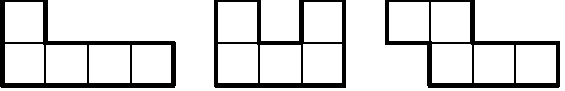
\includegraphics[scale=0.35]{34.png}}
\end{figure}
\end{center}
138. Представьте число 533533533533 в виде произведения как можно большего числа различных натуральных сомножителей.\\
139. Представьте число 517517517517 в виде произведения как можно большего числа различных натуральных сомножителей.\\
140. Четыре спортсмена участвовали в забеге. Оказалось, что Иванов прибежал раньше Петрова, а Васильев --- позже Борисова. Обведите заведомо ложные утверждения:\\
а) Забег выиграл Васильев;\\
б) Иванов прибежал раньше Борисова;\\
в) Последним прибежал не Иванов и не Васильев;\\
г) Если Петров прибежал раньше Васильева, то Петров был последним.\\
141. Четыре толстяка соревновались, кто больше съест пирожных. Оказалось, что Дмитрий съел больше, чем Алексей, а Сергей --- меньше, чем Борис. Обведите заведомо истинные утверждения:\\
а) Алексей съел меньше всех пирожных;\\
б) Дмитрий съел больше, чем Борис;\\
в) Меньше всех съел не Дмитрий и не Сергей;\\
г) Если Алексей съел больше Бориса, то Сергей съел меньше всех.\\
142. У квадрата со стороной 20 см вырезали внутреннюю часть, оставив только каёмку шириной две клеточки. Сколько клеток в этой каёмке? Сторона одной клеточки равна половине сантиметра.\\
143. У квадрата со стороной 17 см вырезали внутреннюю часть, оставив только каёмку шириной три клеточки. Сколько клеток в этой каёмке? Сторона одной клеточки равна половине сантиметра.\\
144. Нарисуйте по сторонам клеточек фигурку, которую можно одним прямолинейным разрезом разделить на пять одинаковых частей. Покажите, как должен идти разрез.\\
145. Нарисуйте по сторонам клеточек фигурку, которую можно одним прямолинейным разрезом разделить на четыре одинаковых части. Покажите, как должен идти разрез.\\
146. В числе 3728924106 зачеркнуть три цифры так, чтобы оставшиеся цифры в том же порядке составили бы наименьшее число. После зачёркивания записать число, которое получается в результате.\\
147. Сколько существует таких пар натуральных чисел $N$ и $N+6,$ что ровно одно из них трёхзначное?\\
148. Вставьте вместо звёздочки цифру так, чтобы 3*44 делилось на 18.\\
149. Начертите прямую и расставьте на ней точки A, B, C и D так, чтобы AB=8 см, CB=5 см, DC=1 см, AC=3 см.\\
150. Сколько треугольников изображено на чертеже?
\begin{center}
\begin{figure}[ht!]
\center{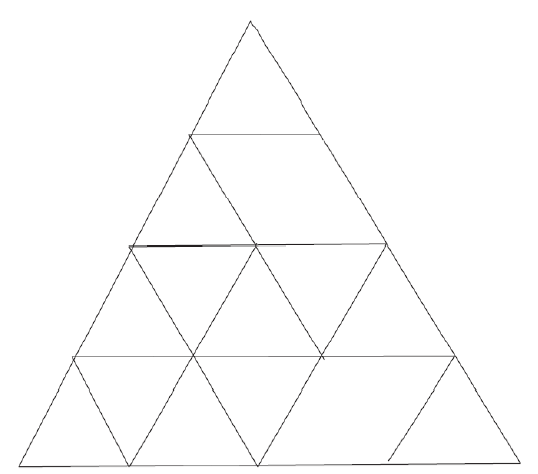
\includegraphics[scale=0.35]{35.png}}
\end{figure}
\end{center}
151. Перечислите все треугольники, которые есть на рисунке.
\begin{center}
\begin{figure}[ht!]
\center{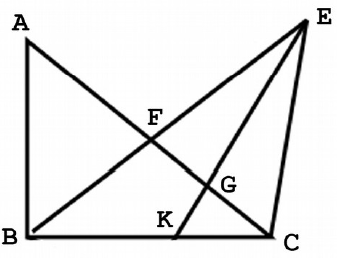
\includegraphics[scale=0.35]{36.png}}
\end{figure}
\end{center}
152. Назовём натуральное число <<замечательным>>, если оно самое маленькое среди натуральных чисел с такой же, как у него, суммой цифр. Чему равно 2017-е <<замечательное>> число?\\
153. Мама купила коробку сахара. дети сначала съели передний слой в 44 кусочка, затем верхний слой --- 77 кусочков и, наконец, боковой слой. Сколько кусочков сахара съели дети? Сколько кусочков сахара было в коробке?\\
154. Екатерина Михайловна покупает тетради для олимпиады. В олимпиаде будет участвовать не то 176 детей, не то 256 детей, она точно не помнит. В магазине есть пачки с любым количеством тетрадей от 2 до 50. Какие пачки следует выбрать Екатерине Михайловне, чтобы купить как можно меньше пачек и на олимпиаде было израсходовано целое число пачек?\\
155. Прямоугольный лист бумаги разделили на четыре части, одна из которых --- квадрат. Периметры серых прямоугольников равны 34 см и 22 см. Найдите: а) периметр; б) площадь листа бумаги.
\begin{center}
\begin{figure}[ht!]
\center{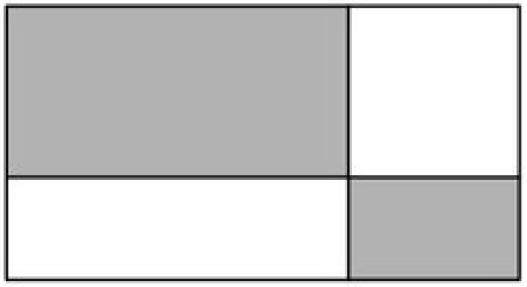
\includegraphics[scale=0.35]{37.png}}
\end{figure}
\end{center}\newpage\noindent
156. Мальвина велела Буратино вместо звёздочек написать различные цифры от 1 до 9 так, чтобы сумма цифр в каждом круге равнялась бы 13. Одну цифру Буратино написал. Помогите ему расставить остальные.
\begin{center}
\begin{figure}[ht!]
\center{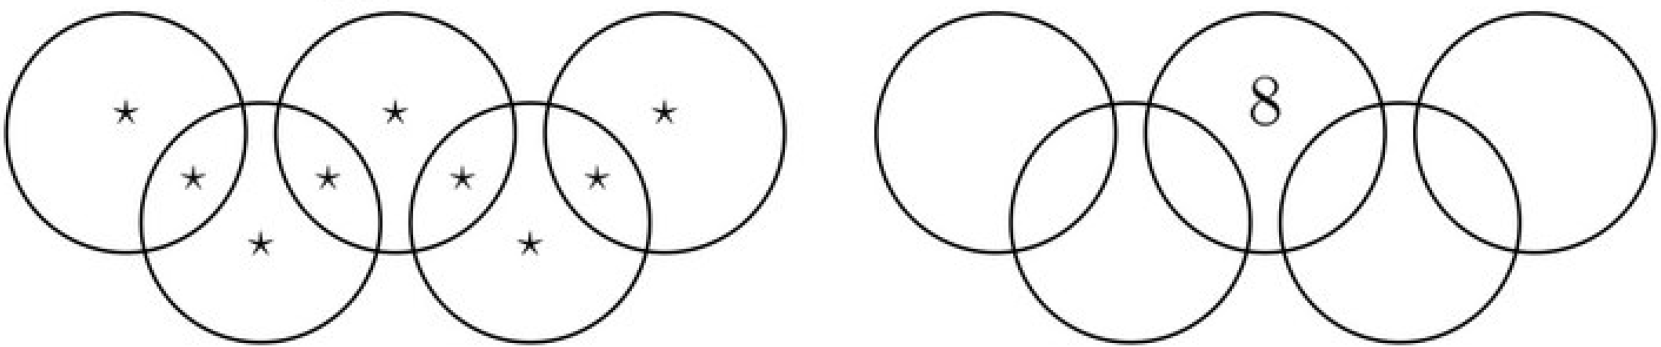
\includegraphics[scale=0.35]{38.png}}
\end{figure}
\end{center}
157. В ящике лежат 100 синих, 100 красных, 100 зелёных и 100 фиолетовых карандашей. Сколько карандашей необходимо достать, не заглядывая в ящик, чтобы среди них обязательно нашлись по крайней мере 1 красный и 1 фиолетовый?\\
158. В стране Лимпопо 9 городов и каждые два города соединены авиалинией. Сколько всего авиалиний в стране Лимпопо?\\
159. Сколько имеется пятизначных чисел, сумма цифр в которых равна трём, причём цифра 1 в записи каждого числа встречается не более одного раза?\\
160. В доме, который заселён только супружескими парами с детьми, проводилась перепись населения. Недобросовестный человек, проводивший перепись, в отчёте указал: <<Взрослых в доме больше, чем детей. У каждого мальчика есть сестра. Мальчиков больше, чем девочек. Бездетных семей нет.>> Найдите в этом отчёте
как можно больше нестыковок и объясните их.\\
161. Расшифруйте ребус на картинке и объясните своё решение.
\begin{center}
\begin{figure}[ht!]
\center{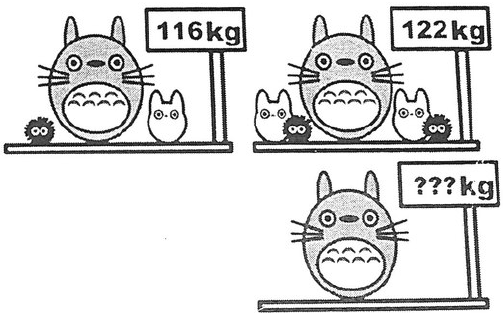
\includegraphics[scale=0.35]{39.png}}
\end{figure}
\end{center}
162. На гранях кубика написаны буквы А, Б, В, Г, Д, Е. На каждой грани 1 буква, при этом все буквы встречаются по 1 разу. Если посмотреть на кубик с одной стороны, то можно увидеть буквы А, В, Г, а если посмотреть ещё с одной стороны, можно увидеть грани Д, Б, В. Какая буква находится на грани, противоположной грани с буквой Е?\\
163. Разделите фигуру на рисунке на 2 одинаковые части.
\begin{center}
\begin{figure}[ht!]
\center{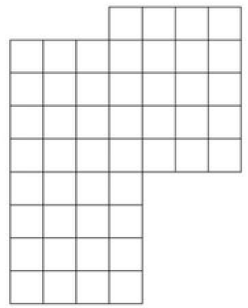
\includegraphics[scale=0.35]{40.png}}
\end{figure}
\end{center}
164. В коробке 30 шариков и кубиков. Среди любых 12 предметов имеется хотя бы один шарик, а среди любых 20 предметов имеется хотя бы один кубик. Сколько шариков и сколько кубиков в коробке?\\
165. Расставьте 8 минусов и 17 плюсов в клетках квадрата $5\times5$ так, чтобы рядом с каждым минусом (т.е. в клетках, соседних по стороне) было ровно 2 плюса.\\
166. Существуют ли два последовательных натуральных числа, сумма цифр каждого из которых делится на 7?\\
167. Пятнадцать рабочих собрали 100 компьютеров. Верно ли, что какие-то два из них собрали одинаковое число компьютеров?\\
168. Выпишите все двузначные числа, которые можно записать с помощью цифр 1, 0 и 3, используя каждую цифру по одному разу. Найдите сумму этих чисел.\\
169. На отрезке AB, равном 32 см, выбрана точка L так, что AL=28 см, и точка K так, что BK=22 см. Найдите отрезок LK.\\
170. В числе 92574063 зачеркните три цифры так, чтобы оставшиеся пять цифр в той же последовательности образовывали как можно меньшее число.\\
171. Есть 6 карточек с цифрой 2. Используя все эти карточки, знаки арифметических действий и, если нужно, скобки, получите число 55.\\
172. Расставь скобки так, чтобы равенство стало верным:\\
а) $7200:90-10\cdot6=540.$\\
б) $8400:3\cdot40+20=90.$\\
в) $210-30:5\cdot3=12.$\\
173. Сколько чётных чисел можно составить, если использовать только цифры 0, 1, 3, 5, причём каждую не более одного раза?\\
174. Сколько различных трёхзначных чисел можно составить из цифр 1, 2, 3, 4?\\
175. Наступил 2017 год. Сколько годов с такой же суммой цифр будет в ближайшие 100 лет?\\
176. В стране Лимпопо 5 городов. Каждые 2 города соединены авиалинией. Сколько всего авиалиний в стране Лимпопо?\\
177. В лавке старьевщика Аладдин увидел три древние лампы: золотую, серебряную и бронзовую, в которых жили добрый и злой джинны. Надпись на золотой лампе гласила: «Здесь живет добрый джинн». На серебряной была надпись «Бронзовая лампа пустая». На бронзовой лампе было написано «Здесь живёт злой джинн». Какую лампу должен выбрать Аладдин, если ему нужен добрый джинн, а все надписи неправильные?\\
178. В одном доме живут четыре друга. Владимир и шофёр старше Сергея. Никита и слесарь занимаются боксом. Электрик – младший из друзей. По вечерам Андрей и токарь играют в лото против Сергея и электрика. Определите профессию каждого из друзей.\\
179. В осеннем лесу росли грибы: мухоморы и белые. Стадо ёжиков прокатилось по грибной полянке и унесло на своих иголках богатую грибную добычу. Внимательная ворона заметила: ёжики унесли столько белых грибов, сколько мухоморов осталось на полянке. Чего было больше: мухоморов, которые сначала росли на полянке, или всех грибов, которые унесли ёжики?\\
180. Вася посчитал число коробочек, в которых один шарик или больше: их оказалось 8; коробочек, в которых больше одного шарика --- 6; больше двух шариков --- 5; больше трёх --- 3; больше четырёх --- 2. Коробочек, в которых больше пяти шариков, не было. Найдите общее число шариков во всех коробках.\\
181. Седьмая часть всех попугаев умеет говорить; пятая часть всех говорящих животных --- попугаи. Кого больше: попугаев или говорящих животных?\\
182. Шестнадцать мальчишек собрались на рыбалку. Известно, что каждый мальчишка, который надел сапоги, надел и кепку. Без сапог оказалось 10 мальчишек, а без кепки --- двое. Каких мальчишек и на сколько больше: тех, кто был в кепке, но без сапог, или тех, кто надел сапоги?\\
183. На лужайке босоногих мальчиков столько же, сколько обутых девочек. Кого на лужайке больше, девочек или босоногих детей?\\
184. В день рождения дяди Фёдора почтальон Печкин хочет выяснить, сколько тому лет. Шарик говорит, что дяде Фёдору больше 11 лет, а кот Матроскин утверждает, что больше 10 лет. Сколько лет дяде Фёдору, если известно, что ровно один из них ошибся?\\
185. Однажды на лестнице была найдена странная тетрадь. В ней было записано сто утверждений:\\
<<В этой тетради ровно одно неверное утверждение>>;\\
<<В этой тетради ровно два неверных утверждения>>;\\
<<В этой тетради ровно три неверных утверждения>>;\\
...\\
<<В этой тетради ровно сто неверных утверждений>>.\\
Есть ли среди этих утверждений верные, и если да, то какие?\\
186. Мачеха, уезжая на бал, дала Золушке мешок, в котором были перемешаны мак и просо, и велела перебрать их. Когда Золушка уезжала на бал, она оставила три мешка: в одном было просо, в другом --- мак, а в третьем --- ещё не разобранная смесь. Чтобы не перепутать мешки, Золушка к каждому из них прикрепила по табличке: <<Мак>>, <<Просо>> и <<Смесь>>. Мачеха вернулась с бала первой и нарочно поменяла местами все таблички так, чтобы на каждом мешке оказалась неправильная надпись. Ученик Феи успел предупредить Золушку, что теперь ни одна надпись на мешках не соответствует действительности. Тогда Золушка достала только одно-единственное зёрнышко из одного мешка и, посмотрев на него, сразу догадалась, где что лежит. Как она это сделала?\\
187. Среди математиков каждый седьмой --- философ, а среди философов каждый девятый --- математик. Кого больше: философов или математиков?\\
188. Прямоугольник периметра 536 см разрезали на два прямоугольника. У одного из новых прямоугольников периметр равен 320 см, а у другого --- 410 см. Найдите площадь того из новых прямоугольников, у кого она меньше.\\
189. Прямоугольник ABCD разделили двумя прямолинейными разрезами на четыре прямоугольника. Известно, что периметр прямоугольника AKFE равен 29 см, периметр прямоугольника EFGD равен 15 см,  а периметр прямоугольника KBHF равен 36 см. Найдите периметр прямоугольника FHCG.\\
190.  К прямоугольнику с двух противоположных сторон приклеили равные квадраты так, что получился новый прямоугольник. Периметр получившегося прямоугольника оказался на 52 см больше периметра первоначального прямоугольника. Найдите периметр каждого квадрата и объясните своё решение.\\
191. Прямоугольник ABCD разделили на четыре меньших прямоугольника с одинаковыми периметрами. Известно, что AB = 18 см, а BC = 16 см. Найдите длины сторон остальных прямоугольников. Обязательно объясните свой ответ.
\begin{center}
\begin{figure}[ht!]
\center{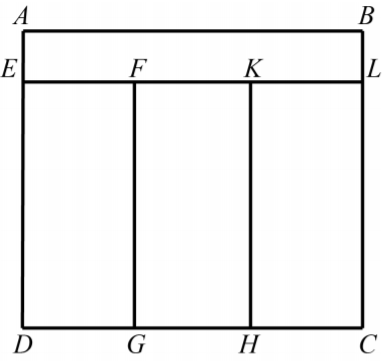
\includegraphics[scale=0.35]{41.png}}
\end{figure}
\end{center}
192. Расстояние между деревнями Орехово и Горохово равно 3 км. В деревне Орехово живут 300 школьников, в деревне Горохово --- 200 школьников. Где следует построить школу, чтобы общее расстояние, пройденное всеми школьниками по дороге в школу, было как можно меньше?\\
193. В деревне A живет 100 школьников, в деревне B живет 50 школьников. Расстояние между деревнями 3 километра. 
В какой точке дороги из A в B надо построить школу, чтобы суммарное расстояние, проходимое всеми школьниками, было бы как можно меньше?\\
194. В ящике красные и жёлтые яблоки. Сколько попыток нужно, чтобы вытащить 2 яблока одного цвета?\\
195. В ящике по 12 яблок красного, жёлтого и зелёного цвета. Сколько попыток дадут 3 яблока одного цвета? Все красные яблоки? Все яблоки разных цветов?\\
196. Наташа и Инна купили по одинаковой коробке чая в пакетиках. Известно, что одного пакетика хватает на две или три чашки чая. Этой коробки Наташе хватило на 41 чашку чая, а Инне --- на 58. Сколько пакетиков было в коробке?\\
197. Найдите все числа, которые уменьшаются в 12 раз при зачёркивании в них последней цифры.\\
198. Одним пакетиком чая можно заварить два или три стакана чая. Мила и Таня разделили коробку чайных пакетиков поровну. Мила заварила 57 стаканов чая, а Таня --- 83 стакана. Сколько пакетиков могло быть в коробке?\\
199. В пакете лежат фрукты. Все, кроме двух, апельсины. Все, кроме двух, яблоки. Все, кроме двух, бананы. Сколько каких фруктов в пакете?\\
200. В корзине лежат 30 рыжиков и груздей. Среди любых 12 грибов имеется хотя бы один рыжик, а среди любых 20 грибов имеется хотя бы один груздь. Сколько рыжиков и сколько груздей в корзине?\\
201. Вася не любит большие числа и вычёркивает цифры. Вычеркните 3 цифры, чтобы получилось число как можно меньше: а) 27818 б) 19107.\\
202. Заяц привёз зайчатам куб, составленный из одинаковых шоколадных кубиков, снаружи покрытый белой глазурью. Мальчики тут же забрали все кубики, у которых были покрыты глазурью ровно 2 грани. Девочки сосчитали, что осталось 168 кубиков. Сколько кубиков забрали зайчата мальчики?\\
203. Деревянный куб покрасили снаружи белой краской, каждое его ребро разделили на 5 равных частей, после чего куб распилили так, что получились маленькие кубики, у которых ребро в 5 раз меньше, чем у исходного куба. Сколько получилось маленьких кубиков, у которых окрашена хотя бы одна грань?\\ 
204. Куб покрасили, а потом распилили так, чтобы получились маленькие кубики, у которых ребро в четыре раза меньше, чем у исходного. У скольких маленьких кубиков окрашены ровно три грани?\\
205. Начнём считать пальцы на правой руке: первый --- мизинец, второй --- безымянный, третий --- средний, четвёртый --- указательный, пятый --- большой, шестой --- снова указательный, седьмой --- снова средний, восьмой --- безымянный, девятый --- мизинец, десятый --- безымянный и т.д. Какой палец будет по счёту 2019-м?\\
206. Трое ребят Аня, Борис и Вера играют в прятки. Водящего они выбирают с помощью считалочки <<На златом крыльце сидели: Царь, царевич, король, королевич, сапожник, портной… Кто ты будешь такой? Говори поскорей, не задерживай добрых и честных людей!>>. Считать начинают с Бориса. Аня очень хочет водить.  В каком порядке им нужно для этого встать?\\
207. Чем оканчивается число 33 в степени 33 (то есть 33 раза умноженное само на себя)?\\
208. Два отца и два сына за завтраком съели 3 яйца причём каждому из них досталось по целому, как такое получилось?\\
209. Сын отца профессора беседует с отцом сына профессора, при этом сам профессор в разговоре не участвует. Как такое может быть?\\
210. В семье 5 братьев и у каждого есть ровно одна сестра. Сколько детей в этой семье?\\
211. Напишите, как будет выглядеть ваше имя в зеркальном отражении.\\
212. Имеется три кучки камней: в первой --- 10, во второй --- 15, в третьей --- 20. За ход разрешается разбить любую кучку на две меньшие. Играют двое. Проигрывает тот, кто не сможет сделать ход. Кто выиграет?\\
213. На столе лежат две стопки монет: в одной из них 30 монет, а в другой --- 20. За ход разрешается взять любое количество монет из одной стопки. Играют двое. Проигрывает тот, кто не сможет сделать ход. Кто из игроков выигрывает при правильной игре?\\
214. Имеется две кучки камней --- по 7 в каждой. Играют двое. За ход разрешается взять любое количество камней, но только из одной кучки. Проигрывает тот, кому нечего брать. Кто из игроков выигрывает при правильной игре?\\
215. Имеются чашечные весы без гирь и 3 одинаковые по внешнему виду монеты, одна из которых фальшивая: она легче настоящих (настоящие монеты одного веса). Сколько надо взвешиваний, чтобы определить фальшивую монету?\\
216. Дано 27 монет, из которых одна фальшивая, причём фальшивая монета легче настоящей. Как за три взвешивания на чашечных весах без гирь определить фальшивую монету?\\
217. Имеются чашечные весы без гирь и 3 одинаковые по внешнему виду монеты. Одна из монет фальшивая, причём неизвестно, легче она настоящих монет или тяжелее (настоящие монеты одного веса). Сколько надо взвешиваний, чтобы определить фальшивую монету? Решите ту же задачу в случаях, когда имеется 4 монеты и 9 монет.\\
218. Сколько всего прапрадедушек и прапрабабушек было у всех ваших прапрадедушек и прапрабабушек?\\
219. Если в записи некоторого натурального числа зачеркнуть последнюю цифру 4, то оно уменьшится на 229. Найти это число.\\
220. Если в записи натурального числа зачеркнуть последнюю цифру 0, то оно уменьшится на 666.Найдите это число.\\
221. Поверхность куба со стороной 6см покрасили снаружи в красный цвет. После этого его распилили на кубики со стороной 1см. У каждого из получившихся кубиков посчитали количество красных граней. У скольких кубиков это количество не равно двум?\\
222. Поверхность куба со стороной 7см покрасили снаружи в красный цвет. После этого его распилили на кубики со стороной 1см. У каждого из получившихся кубиков посчитали количество красных граней. У скольких кубиков это количество не равно двум?\\
223. Расставьте в клетках фигуры числа от 2 до 11, каждое по одному разу, так, чтобы в любой полоске из трёх клеток (горизонтальной или вертикальной) сумма делилась на 3.
\begin{center}
\begin{figure}[ht!]
\center{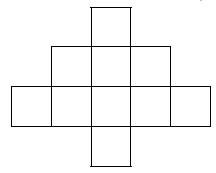
\includegraphics[scale=0.35]{166.png}}
\end{figure}
\end{center}
224. Расставьте в клетках фигуры числа от 1 до 10, каждое по одному разу, так, чтобы в любой полоске из трёх клеток (горизонтальной или вертикальной) сумма делилась на 3.
\begin{center}
\begin{figure}[ht!]
\center{\includegraphics[scale=0.35]{16.png}}
\end{figure}
\end{center}
225. На клетчатой бумаге поставлены точки. Соедините их отрезками таким образом, чтобы каждая точка была вершиной квадрата.
\begin{center}
\begin{figure}[ht!]
\center{\includegraphics[scale=0.3]{01.png}}
\end{figure}
\end{center}
226. У Винтика и Шпунтика на 4 коробках были таблички <<Гайки и отвёртки>>, <<Молотки>>, <<Отвёртки>>, <<Гайки и молотки>>. Незнайка случайно перепутал таблички так, что ни в одной из коробок не лежит ничего из того, что упомянуто на табличке. Что лежит в коробке с надписью <<Отвёртки>>?\\
227. На гранях кубика написаны 6 натуральных чисел, три из которых видны на рисунке. Известно, что произведение чисел, написанных на противоположных гранях, одинаковы. Какое наименьшее значение может принимать сумма всех чисел на гранях кубика?
\begin{center}
\begin{figure}[ht!]
\center{\includegraphics[scale=0.25]{02.png}}
\end{figure}
\end{center}
228. Запишите наибольшее шестизначное число, для которого выполняются все следующие условия:\\
1) все цифры этого числа различны;\\
2) если умножить любую из его цифр на цифру, стоящую в разряде десятков, в результате будет одно и то же число;\\
3) первая и третья цифра делятся на вторую цифру.\\
229. Запишите наименьшее шестизначное число, для которого выполняются все следующие условия:\\
1) все цифры этого числа различны;\\
2) если умножить любую из его цифр на цифру, стоящую в разряде сотен, в результате будет одно и то же число;\\
3) третья и пятая цифра делятся на шестую цифру.\\
230. Сколько существует пятизначных чисел с суммой цифр три?\\
231. Сколько существует четырёхзначных чисел с суммой цифр четыре?\\
232. Кузнечик прыгает по клеточной полоске двумя способами: первым $(1)$ --- вперёд на пять клеток, вторым $(2)$ --- назад на три клетки. При этом он красит в чёрный цвет каждую клетку,  в которой он побывал. Запишите последовательности команд, благодаря которой он покрасит только клетки с первой по 10. Он начинает в клетке с номером 1.\\
233. Кузнечик прыгает по клеточной полоске двумя способами: первым $(1)$ --- вперёд на семь клеток, вторым $(2)$ --- назад на четыре клетки. При этом он красит в чёрный цвет каждую клетку в которой он побывал. Запишите последовательности команд, благодаря которой он покрасит только клетки с первой по четырнадцатую. Он начинает в клетке с номером 1.\\
234. На острове живут рыцари и лжецы. Путник встретил троих островитян и спросил каждого из них: <<Сколько рыцарей среди твоих спутников?>>. Первый сказал --- <<ни одного>>,  второй сказал --- <<один>>. Что сказал третий?\\
235. На острове живут рыцари и лжецы. Путник встретил троих островитян и спросил каждого из них: <<Сколько рыцарей среди твоих спутников?>>. Первый сказал --- <<один>>,  второй сказал --- <<ни одного>>. Что сказал третий?\\
236. Нарисуйте несколько прямоугольников так, чтобы все внутренние части оказались треугольниками, и их было не меньше шести.\\
237. Паша построил четырёхуровневую пирамиду, так что каждый кубик опирается на четыре других нижних кубика. Саша хочет увеличить пирамиду в высоту на два этажа. Сколько кубиков ему потребуется?\\
238. С полудня до полуночи Кот Учёный спит под дубом, а с полуночи до полудня рассказывает сказки. Кот повесил на дубе плакат: <<Через час я буду делать то же самое, что делал два часа назад>>. Сколько часов в сутки эта надпись верна?\\
239. С полудня до полуночи Кот Учёный спит под дубом, а с полуночи до полудня рассказывает сказки. Кот повесил на дубе плакат: <<Через два часа я буду делать то же самое, что делал три часа назад>>. Сколько часов в сутки эта надпись верна?\\
240. Имеются три гири 1кг, 2кг, 9кг. Какие веса можно взвесить с помощью этих гирь на весах с двумя чашами, если можно класть гири на обе чаши? Перечислите все варианты в порядке возрастания.\\
241. Имеются три гири 1кг, 2кг, 10кг. Какие веса можно взвесить с помощью этих гирь на весах с двумя чашами, если можно класть гири на обе чаши? Перечислите все варианты в порядке возрастания.\\
242. Сколько существует натуральных чисел $N$ таких, что ровно два из трёх чисел $N, N+10, N+25$ являются трёхзначными?\\
243. Сколько существует натуральных чисел $N$ таких, что ровно два из трёх чисел $N, N+15, N+20$ являются трёхзначными?\\
244. Число называется палиндромом, если оно читается слева направо и справа налево одинаково (например, 1221 и 15651 --- палиндромы). Будем называть число {\bf красивым}, если числа, большие его на 3 и на 5, оба являются палиндромами. Придумайте какое-нибудь красивое четырёхзначное число.\\
245. Число называется палиндромом, если оно читается слева направо и справа налево одинаково (например, 1221 и 15651 --- палиндромы). Будем называть число {\bf красивым}, если числа, меньшие его на 3 и на 5, оба являются палиндромами. Придумайте какое-нибудь красивое четырёхзначное число.\\
246. Про четырёхзначное число известно, что сумма его цифр равна разности 2019 и самого числа. Найдите все такие числа.\\
247. Про четырёхзначное число известно, что сумма его цифр равна разности 2021 и самого числа. Найдите все такие числа.\\
248. Сумма 15 натуральных чисел равна 18. Чему может быть равно произведение?\\
249. Сумма 16 натуральных чисел равна 19. Чему может быть равно произведение?\\
250. Найдите все решения ребуса ДУБ+ДУБ+ДУБ=БББ+36. (Одинаковые буквы означают одинаковые цифры, разные буквы --- разные цифры.)\\
251. Найдите все решения ребуса МЯУ+МЯУ+МЯУ=УУУ+48. (Одинаковые буквы означают одинаковые цифры, разные буквы --- разные цифры.)\\
252. По кругу стоят 30 детей. Дед Мороз дарит им подарки: первому 1, второму 2, следующему 1, потом 2 и так далее. Всего он подарил 55 подарков (пока не кончились подарки). Сколько детей получили ровно 2 подарка?\\
253. По кругу стоят 32 ребёнка. Дед Мороз дарит им подарки: первому 4, второму 2, следующему 4, потом 2 и так далее. Всего он подарил 112 подарков (пока не кончились подарки). Сколько детей получили ровно 4 подарка?\\
254. На рисунке показана полоска $2\times 8,$ её периметр равен 20. Если удалить клетки A и C или B и C, то она развалится на части, а если удалить клетки A и B, то периметр оставшейся части станет равен 22. Сколько есть способов удалить из полоски $2\times 20$ две клетки так, чтобы она осталась целой, а периметр оставшейся части был равен 48?
\begin{figure}[ht!]
\center{\includegraphics[scale=0.35]{05.png}}
\end{figure}\\
255. На рисунке показана полоска $2\times 8,$ её периметр равен 20. Если удалить клетки A и C или B и C, то она развалится на части, а если удалить клетки A и B, то периметр оставшейся части станет равен 22. Сколько есть способов удалить из полоски $2\times 21$ две клетки так, чтобы она осталась целой, а периметр оставшейся части был равен 50?
\begin{figure}[ht!]
\center{\includegraphics[scale=0.35]{05.png}}
\end{figure}\\
256. Аня посчитала сумму всех трёхзначных чисел, оканчивающихся на 9, Вася вычислил сумму всех трёхзначных чисел, последняя цифра которых 8. Саша нашёл сумму всех трёхзначных чисел, оканчивающихся на 4, а Дима сложил все трёхзначные числа, оканчивающиеся двойкой. Аня и Саша сложили свои результаты, а Вася и Дима --- свои. У кого сумма оказалась больше? На сколько?\\
257. Аня посчитала сумму всех трёхзначных чисел, оканчивающихся на 8, Вася вычислил сумму всех трёхзначных чисел, последняя цифра которых 9. Саша нашёл сумму всех трёхзначных чисел, оканчивающихся на 4, а Дима сложил все трёхзначные числа, оканчивающиеся двойкой. Аня и Саша сложили свои результаты, а Вася и Дима --- свои. У кого сумма оказалась больше? На сколько?\\
258. У какого числа от 2381895 до 2761984 самая большая сумма цифр?\\
259. У какого числа от 3497029 до 3813472 самая большая сумма цифр?\\
260. Придумайте три числа с суммой 83, произведение которых заканчивается на 4 нуля.\\
261. Придумайте три числа с суммой 91, произведение которых заканчивается на 4 нуля.\newpage\noindent
262. \begin{figure}[ht!]
\center{\includegraphics[scale=0.3]{rss.png}}
\end{figure}\\
На рисунке показан прямоугольник $2\times4.$ Если удалить клетки $A$ и $C$ или $B$ и $C,$ то он развалится на две части, а если удалить клетки $A$ и $B,$ то не развалится. А какое наименьшее количество клеток в прямоугольнике $5\times7$ нужно удалить, чтобы он развалился на части?\\
263. \begin{figure}[ht!]
\center{\includegraphics[scale=0.3]{rss.png}}
\end{figure}\\
На рисунке показан прямоугольник $2\times4.$Если удалить клетки $A$ и $C$ или $B$ и $C,$ то он развалится на две части, а если удалить клетки $A$ и $B,$ то не развалится. А какое наименьшее количество клеток в прямоугольнике $5\times6$ нужно удалить, чтобы он развалился на части?\\
264. У нечётного четырёхзначного числа вычислили сумму его последней цифры и трёхзначного числа, получаемого вычёркиванием последней цифры из данного. Получилось 203. Каким могло быть исходное четырёхзначное число?\\
265. У чётного четырёхзначного числа вычислили сумму его последней цифры и трёхзначного числа, получаемого вычёркиванием последней цифры из данного. Получилось 204. Каким могло быть исходное четырёхзначное число?\\
266. В последовательности $1, 2, 2, 4, 8, 2, 6, \ldots$ каждая цифра равна последней цифре произведения предыдущих двух цифр. Как видно, на 4-м месте стоит цифра 4. А какая цифра стоит на 2021-м месте?\\
267. В последовательности $2, 1, 2, 2, 4, 8, 2, \ldots$ каждая цифра равна последней цифре произведения предыдущих двух цифр. Как видно, на 6-м месте стоит цифра 8. А какая цифра стоит на 2021-м месте?\\
268. На электронных часах высвечивается $11:13:33.$ Через какое время впервые пять из шести цифр на табло часов окажутся одинаковыми?\\
269. На электронных часах высвечивается $11:14:44.$ Через какое время впервые пять из шести цифр на табло часов окажутся одинаковыми?\\
270. Если из квадрата $3\times3$ вырезать центральную клетку, то в нём будет 8 внутренних перегородок. Если же из квадрата $4\times4$ вырезать дырку $2\times2,$ то будет 12 внутренних перегородок. Из прямоугольника $100\times200$ вырезали две непересекающиеся и несоприкасающиеся квадратные дырки $7\times7.$ Сколько осталось внутренних перегородок?\\
271. Если из квадрата $3\times3$ вырезать центральную клетку, то в нём будет 8 внутренних перегородок. Если же из квадрата $4\times4$ вырезать дырку $2\times2,$ то будет 12 внутренних перегородок. Из прямоугольника $100\times200$ вырезали две непересекающиеся и несоприкасающиеся квадратные дырки $8\times8.$ Сколько осталось внутренних перегородок?\\
272. В углу прямоугольника $3\times5$ стоит кубик (размер грани кубика совпадает с клеткой). У данного кубика сильно испачкана одна грань. Можно перекатывать кубик через ребро, при этом запрещено выкатывать его за пределы прямоугольника и ставить на клетку, на которой кубик уже стоял. Придумайте способ испачкать как можно больше клеток прямоугольника. Какая именно грань кубика запачкана, вы можете выбрать сами. В каждой клетке прямоугольника запишите, какой по счёту эта клетка окажется под кубиком (в клетке, на которой кубик стоит изначально, запишите число 1). В ответ запишите число испачканных клеток.
\begin{center}
\begin{figure}[ht!]
\center{\includegraphics[scale=0.35]{kub1.png}}
\end{figure}
\end{center}
273. В углу прямоугольника $3\times6$ стоит кубик (размер грани кубика совпадает с клеткой). У данного кубика сильно испачкана одна грань. Можно перекатывать кубик через ребро, при этом запрещено выкатывать его за пределы прямоугольника и ставить на клетку, на которой кубик уже стоял. Придумайте способ испачкать как можно больше клеток прямоугольника. Какая именно грань кубика запачкана, вы можете выбрать сами. В каждой клетке прямоугольника запишите, какой по счёту эта клетка окажется под кубиком (в клетке, на которой кубик стоит изначально, запишите число 1). В ответ запишите число испачканных клеток.
\begin{center}
\begin{figure}[ht!]
\center{\includegraphics[scale=0.35]{kub2.png}}
\end{figure}
\end{center}
274. Муравьишка ползёт по поверхности кубика (вертикально или горизонтально) из точки $A$ в точку $B$ по пути, отмеченному стрелками. Чему равна длина этого пути, если ребро кубика равно 15 см?
\begin{center}
\begin{figure}[ht!]
\center{\includegraphics[scale=0.35]{mur.png}}
\end{figure}
\end{center}
275. \begin{center}
\begin{figure}[ht!]
\center{\includegraphics[scale=0.35]{treug.png}}
\end{figure}
\end{center}
Сколько клеточек составляет площадь фигуры?\\
276. Винни Пух и Пятачок проверяют запасы мёда у Кролика. Они подсчитали, что у Кролика всего 7 горшочков цветочного мёда, 6 горшочков липового мёда и 3 горшочка гречишного мёда. Увлёкшись проверкой, Винни Пух съел 2 горшочка мёда. Что могло при этом получиться? ({\it выберите один или несколько возможных вариантов})\\
1. У Кролика не осталось гречишного мёда.\\
2. Горшочков липового мёда стало меньше, чем гречишного.\\
3. Горшочков всех видов мёда стало поровну.\\
4. Горшочков двух видов мёда стало поровну.\\
5. Горшочков с цветочным мёдом стало больше, чем всех остальных вместе.\\
6. Горшочков какого-то вида мёда стало ровно половина от всех оставшихся горшочков мёда.\newpage\noindent
277. \begin{center}
\begin{figure}[ht!]
\center{\includegraphics[scale=0.35]{pol.png}}
\end{figure}
\end{center}
На полу лежат четыре прямоугольных ковра, перекрывая друг друга. Напишите номера всех областей, которые покрыты ровно тремя из них.\newpage\noindent
278. \begin{center}
\begin{figure}[ht!]
\center{\includegraphics[scale=0.35]{giri.png}}
\end{figure}
\end{center}
С гирьками проделали 3 взвешивания. Какая гирька самая тяжёлая и какая самая лёгкая?\\
279. Ёжик загадал четырёхзначное число $A,$ все цифры которого различны, а Крош его угадывает. Крош уже узнал, что:\\
 --- число 8702 содержит ровно одну цифру числа $A,$ причём на правильном месте;\\
 --- число 8237 содержит ровно две цифры числа $A,$ причём одна на правильном месте, а вторая на неправильном месте;\\
 --- число 7024 содержит ровно одну цифру числа $A,$ причём на правильном месте;\\
 --- число 7130 содержит ровно две цифры числа $A,$ причём обе на неправильных местах.\\
 Какое число загадал Ёжик?\\
  {\it {\textbf {Запишите только ответ, пояснять его не нужно.}}}\\
280. Робот Федя ходит по клетчатому полю. Каждый раз после перехода в соседнюю клетку Федя поворачивает налево или направо. Поворот налево занимает у него 5 секунд, а поворот направо --- 3 секунды. После этого 7 секунд он идёт до следующего поворота. Он начал своё движение с поворота налево и закончил перед поворотом. После старта Федя путешествовал по полю 2 минуты и 2 секунды. Сколько раз он при этом мог поворачивать направо? {\textbf {Найдите все возможные варианты.}}\\
281. Найдите какое-нибудь натуральное число, которое делится на 12, 35 и 15 одновременно.\\
282. Найдите какое-нибудь натуральное число, которое делится на 6, 8, 9 и 21 одновременно.\\
283. Нарисуйте 5 отрезков так, чтобы можно было закрасить (внутри) синим цветом 5 треугольников и красным один пятиугольник. На плоскости не должно быть точек двух цветов сразу. Отметьте точками или буквами начала и концы отрезков.\\
284. Нарисуйте на плоскости 7 отрезков так, чтобы можно было закрасить (внутри) синим цветом 2 квадрата и красным один пятиугольник. На плоскости не должно быть точек двух цветов сразу. Отметьте точками или буквами начала и концы отрезков.\\
285. Анатолий выписал на доску все двузначные числа, делящиеся на 4. Сколько раз он написал цифру 6?\\
286. Петя выписал на доску все двузначные числа, делящиеся на 4. Сколько раз он написал цифру 8?\\
287. От прямоугольника отрезали с двух противоположных сторон по квадрату, так чтобы эти квадраты не имели общих сторон. В результате получился прямоугольник с периметром на 24 меньше. Найдите периметр каждого квадрата.\\
288. От прямоугольника отрезали с двух противоположных сторон по квадрату, так чтобы эти квадраты не имели общих сторон. В результате получился прямоугольник с периметром на 36 меньше. Найдите периметр каждого квадрата.\\
289. Вчера было 15.05 и номер дня был ровно в три раза больше номера месяца. Сколько таких дней в 2021 году?\\
290. Скоро будет 20.05 и номер дня будет ровно в четыре раза больше номера месяца. Сколько таких дней в 2021 году?\\
291. Саша по вторникам и субботам называет числа правильно, по понедельникам и пятницам преувеличивает числа в 3 раза, а в остальные дни уменьшает числа на 1. Он шесть дней подряд отвечал на вопрос <<Какого числа ты родился?>> Мог ли он назвать числа 2, 3, 3, 3, 9, 9 в каком-то порядке? Если да --- покажите как, если нет --- объясните почему.\\
292. Представьте число 2547 в виде суммы трёх трёхзначных чисел таких, что в их записи все 9 цифр были бы различны.\\
293. Представьте число 2543 в виде суммы трёх трёхзначных чисел таких, что в их записи все 9 цифр были бы различны.\\
294. Сколько существует пятизначных чисел, в записи каждого из которых есть цифра 5 или цифра 7?\\
295. Сколько существует пятизначных чисел, в записи каждого из которых есть цифра 2 или цифра 4?\\
296. У четырёхзначного числа вычислили сумму его последней цифры и трёхзначного числа, получаемого вычёркиванием предпоследней цифры из данного. Получилось 204. Каким могло быть исходное четырёхзначное число? Выберите из них то, у которого наибольшая сумма цифр и запишите его в ответ.\\
297. У четырёхзначного числа вычислили сумму его последней цифры и трёхзначного числа, получаемого вычёркиванием предпоследней цифры из данного. Получилось 206. Каким могло быть исходное четырёхзначное число? Выберите из них то, у которого наибольшая сумма цифр и запишите его в ответ.\\
298. На электронных часах высвечивается $11:30:00.$ Какое время назад последний раз пять из шести цифр на табло часов были одинаковыми?\\
299. На электронных часах высвечивается $22:40:00.$ Какое время назад последний раз пять из шести цифр на табло часов были одинаковыми?\\
300. Если из квадрата $3\times3$ вырезать центральную клетку, то в нём будет 8 внутренних перегородок. Если же из квадрата $4\times4$ вырезать дырку $2\times2,$ то будет 12 внутренних перегородок. Из квадрата вырезали пять непересекающихся и не соприкасающихся дырок $2\times2.$ В полученной фигуре оказалось ровно 20952 внутренних перегородки. Чему равна сторона квадрата?\\
301. Если из квадрата $3\times3$ вырезать центральную клетку, то в нём будет 8 внутренних перегородок. Если же из квадрата $4\times4$ вырезать дырку $2\times2,$ то будет 12 внутренних перегородок. Из квадрата вырезали пять непересекающихся и не соприкасающихся дырок $2\times2.$ В полученной фигуре оказалось ровно 21364 внутренних перегородки. Чему равна сторона квадрата?\\
302. Каждый четвероклассник пожал руку четырём пятиклассникам и шести четвероклассникам, при этом каждый пятиклассник пожал руку шести четвероклассникам и семи пятиклассникам. Сколько четвероклассников, если всего в двух классах 50 человек?\\
303. Каждый четвероклассник пожал руку трём пятиклассникам и шести четвероклассникам, при этом каждый пятиклассник пожал руку семи четвероклассникам и пяти пятиклассникам. Сколько пятиклассников, если всего в двух классах 50 человек?\\
304. \begin{figure}[ht!]
\center{\includegraphics[scale=0.35]{tab.png}}
\end{figure}\\
Расставьте в каждую клетку таблицы $3\times6$ букву К, А или С так, чтобы у каждой К было 4 соседа А, а у каждой С было ровно два соседа А, а у каждой А среди соседей есть и К, и С. Соседи считаются только по стороне.\\
305. \begin{figure}[ht!]
\center{\includegraphics[scale=0.35]{tab.png}}
\end{figure}\\
Расставьте в каждую клетку таблицы $3\times6$ букву М, Я или П так, чтобы у каждой М было 4 соседа Я, а у каждой П было ровно два соседа Я, а у каждой Я среди соседей есть и М, и П. Соседи считаются только по стороне.\\
306. На схеме изображён пустой стальной кубик со стороной 1 метр. На каждой его грани нарисовали 25 одинаковых квадратиков и просверлили три дырки как показано на рисунке. Кубик можно ставить на другие грани, но нельзя дыркой вниз. Какое наибольшее количество литров воды можно налить в этот кубик? Напомним, что литр --- это дециметр кубический.
\begin{figure}[ht!]
\center{\includegraphics[scale=0.35]{kub.png}}
\end{figure}\\
307. На схеме изображён пустой стальной кубик со стороной 1 метр. На каждой его грани нарисовали 25 одинаковых квадратиков и просверлили три дырки как показано на рисунке. Кубик можно ставить на другие грани, но нельзя дыркой вниз. Какое наибольшее количество литров воды можно налить в этот кубик? Напомним, что литр --- это дециметр кубический.
\begin{figure}[ht!]
\center{\includegraphics[scale=0.35]{kukub.png}}
\end{figure}\\
308. На рисунке изображены углы. Запишите в ответ номера углов в следующем порядке: острый, прямой, тупой.\\
\begin{figure}[ht!]
\center{\includegraphics[scale=0.35]{ugl2.png}}
\end{figure}\newpage\noindent
309. На рисунке изображены углы. Запишите в ответ номера углов в следующем порядке: острый, прямой, тупой.\\
\begin{figure}[ht!]
\center{\includegraphics[scale=0.35]{ugl1.png}}
\end{figure}\\
310. На трёх непрозрачных банках написано: {\bf <<Горох>>; <<Не горох>>; <<Горох или пуговицы>>.} Известно, что все эти надписи ложны. При этом в банках лежат горох, мука и пуговицы. В которой из банок лежит мука?\\
311. На трёх непрозрачных банках написано: {\bf <<Крупа>>; <<Не крупа>>; <<Крупа или гайки>>.} Известно, что все эти надписи ложны. При этом в банках лежат крупа, сахар и гайки. В которой из банок лежит сахар?\\
312. Отрезки $AB,\ BC$ и $CK$ расположены на одной прямой, причём точка $C$ лежит между точками $A$ и $B,$ а точка $B$ между точками $C$ и $K.$Чему равна длина отрезка $AK,$ если $AB=10$ см, $BC=3$ см, $CK=8$ см?\\
313. Отрезки $MP,\ PK$ и $KA$ расположены на одной прямой, причём точка $K$ лежит между точками $M$ и $P,$ а точка $P$ между точками $A$ и $K.$Чему равна длина отрезка $AM,$ если $MP=12$ см, $PK=2$ см, $KA=6$ см?\\
314. Дано число 29546381. Вычеркните в нём три цифры так, чтобы оставшееся число было наибольшим чётным. Результат запишите.\\
315. Дано число 29546318. Вычеркните в нём три цифры так, чтобы оставшееся число было наименьшим нечётным. Результат запишите.\\
316. Найдите периметр самого большого прямоугольника на рисунке, если площадь закрашенного квадрата равна $64\text{ см}^2.$ Все 5 фигур, из которых составлен большой прямоугольник --- квадраты.\\
\begin{figure}[ht!]
\center{\includegraphics[scale=0.35]{pram1.png}}
\end{figure}\\
317. Найдите периметр самого большого прямоугольника на рисунке, если площадь закрашенного квадрата равна $16\text{ см}^2.$ Все 5 фигур, из которых составлен большой прямоугольник --- квадраты.\\
\begin{figure}[ht!]
\center{\includegraphics[scale=0.35]{pram2.png}}
\end{figure}\\
318. Для двух групп экскурсантов заказали 472 конфеты и 118 бутербродов. Количество людей в группах отличается не более, чем на 2. В каждой группе меньше 35 людей. Сколько людей в каждой группе, если ни один человек не получит ни конфет, ни бутербродов больше, чем другой? Если в группах разное количество людей, запишите в ответ меньшее число.\\
319. Для двух групп экскурсантов заказали 427 конфет и 122 бутерброда. Количество людей в группах отличается не более, чем на 2. В каждой группе меньше 35 людей. Сколько людей в каждой группе, если ни один человек не получит ни конфет, ни бутербродов больше, чем другой? Если в группах разное количество людей, запишите в ответ большее число.\\
320. Замените звёздочки цифрами так, чтобы равенство стало верным и все семь цифр были различными: $**+**=175.$\\
321. Замените звёздочки цифрами так, чтобы равенство стало верным и все семь цифр были различными: $**+**=176.$\\
322. Серёжа согнул две проволоки так, как показано на рисунке, и наложил их друг на друга, не разгибая. Какова наибольшая возможная длина их общей (совпавшей) части, если 2 клеточки равны 1 см?\\
\begin{figure}[ht!]
\center{\includegraphics[scale=0.35]{prov1.png}}
\end{figure}\\
323. Серёжа согнул две проволоки так, как показано на рисунке, и наложил их друг на друга, не разгибая. Какова наибольшая возможная длина их общей (совпавшей) части, если 1 клеточка равна 1 см?\\
\begin{figure}[ht!]
\center{\includegraphics[scale=0.35]{prov2.png}}
\end{figure}\\
324. У Кроша есть шесть карточек, на которых записаны числа 415, 41, 7, 19, 78, 3. Расположите карточки в ряд так, чтобы получившееся одиннадцатизначное число было наименьшим из возможных.\\
325. У Кроша есть шесть карточек, на которых записаны числа 435, 43, 7, 13, 74, 3. Расположите карточки в ряд так, чтобы получившееся одиннадцатизначное число было наименьшим из возможных.\\
326. Отрезок, равный 28 см, разделён на три (возможно, неравных) отрезка. Расстояние между серединами крайних отрезков равно 16 см. Найдите длину среднего отрезка.\\
327. Отрезок, равный 30 см, разделён на три (возможно, неравных) отрезка. Расстояние между серединами крайних отрезков равно 16 см. Найдите длину среднего отрезка.\\
328. Перед Вами марсианская единица измерения площади --- шкрындла. Измерьте приведённые ниже фигуры в
шкрындлах.\\
\begin{figure}[ht!]
\center{\includegraphics[scale=0.35]{sc1.png}}
\end{figure}\\
329. Перед Вами марсианская единица измерения площади --- шкрындла. Измерьте приведённые ниже фигуры в
шкрындлах.\\
\begin{figure}[ht!]
\center{\includegraphics[scale=0.35]{sc2.png}}
\end{figure}\\
330. Чему равняется сумма цифр числа $1\underbrace{00\ldots00}_{2022}-2022?$\\
331. Чему равняется сумма цифр числа $1\underbrace{00\ldots00}_{2021}-2021?$\\
332. Петя посчитал сумму первой тысячи натуральных чисел, делящихся на 6. А Вася посчитал сумму первой тысячи нечётных натуральных чисел, делящихся на 3. Найдите разность чисел, получившихся у мальчиков.\\
333. Петя посчитал сумму первой тысячи натуральных чисел, делящихся на 10. А Вася посчитал сумму первой тысячи нечётных натуральных чисел, делящихся на 5. Найдите разность чисел, получившихся у мальчиков.\\
334. Крош и Бараш в $9:00$ одновременно вышли друг к другу в гости. Каждый из них идёт с постоянной скоростью. Через полчаса они встретились в первый раз, поздоровались и пошли дальше. Добравшись до домика друг друга и убедившись, что там никого нет, оба повернули обратно. Во сколько Крош и Бараш встретятся второй раз?\\
335. Крош и Бараш в $10:00$ одновременно вышли друг к другу в гости. Каждый из них идёт с постоянной скоростью. Через час они встретились в первый раз, поздоровались и пошли дальше. Добравшись до домика друг друга и убедившись, что там никого нет, оба повернули обратно. Во сколько Крош и Бараш встретятся второй раз?\\
336. На доске написано трёхзначное число. Петя поменял в нём первую и последнюю цифру местами и написал полученное число на доске. Оказалось, что разница написанных чисел --- это трёхзначное число. Найдите вторую цифру разницы написанных чисел.\\
337. В примере на сложение $\star54\star\star+\star82\star\star=10\star793$ звёздочками заменены некоторые цифры (не обязательно одинаковые). Найдите сумму этих семи цифр.\\
338. В примере на сложение $\star62\star\star+\star73\star\star=11\star691$ звёздочками заменены некоторые цифры (не обязательно одинаковые). Найдите сумму этих семи цифр.\\
339. Придумайте три различных трёхзначных числа с суммой 817, которые отличаются только первой цифрой. В ответ запишите все три числа.\\
340. Придумайте три различных трёхзначных числа с суммой 917, которые отличаются только первой цифрой. В ответ запишите все три числа.\\
341. Сколько существует пятизначных чисел, в записи каждого из которых первая цифра больше третьей?\\
342. Сколько существует пятизначных чисел, в записи каждого из которых первая цифра больше четвёртой?\\
343. В углу квадрата $2025\times2025$ живёт жук, а в противоположном углу этого квадрата находится его школа. Жук умеет за один шаг переходить в соседний по стороне или вершине квадратик. Тем самым, чтобы добраться до школы, ему надо сделать 2024 шага. В некоторый момент в центральном квадратике $1\times1$ случилась авария, и теперь ему до школы 2024 шага. Сколько шагов надо будет сделать жуку до школы, если авария разрастётся до квадрата $7\times7$ (центры аварии и большого квадрата совпадают)?\\
344. В углу квадрата $2023\times2023$ живёт жук, а в противоположном углу этого квадрата находится его школа. Жук умеет за один шаг переходить в соседний по стороне или вершине квадратик. Тем самым, чтобы добраться до школы, ему надо сделать 2022 шага. В некоторый момент в центральном квадратике $1\times1$ случилась авария, и теперь ему до школы 2023 шага. Сколько шагов надо будет сделать жуку до школы, если авария разрастётся до квадрата $7\times7$ (центры аварии и большого квадрата совпадают)?\newpage\noindent
345. На квадратном поле $4\times4$ клетки растут цветы, число цветов в каждой клетке указано на схеме. Вася начинает с левой нижней клетки (с числом 8) и, переходя каждый раз в соседнюю справа или сверху, добирается до правой верхней клетки, собирая цветы с клеток, на которых побывал. Сколько есть маршрутов, на которых Вася соберёт ровно 25 цветков?\\
\begin{figure}[ht!]
\center{\includegraphics[scale=0.35]{flow1.png}}
\end{figure}\\
346. На квадратном поле $4\times4$ клетки растут цветы, число цветов в каждой клетке указано на схеме. Вася начинает с левой нижней клетки (с числом 2) и, переходя каждый раз в соседнюю справа или сверху, добирается до правой верхней клетки, собирая цветы с клеток, на которых побывал. Сколько есть маршрутов, на которых Вася соберёт ровно 43 цветка?\\
\begin{figure}[ht!]
\center{\includegraphics[scale=0.35]{flow2.png}}
\end{figure}\\
347. На электронном табло высвечивается время $23:23:23.$ В какое время после этого в шестой раз все цифры на табло будут различными?\\
348. На электронном табло высвечивается время $12:12:12.$ В какое время после этого в седьмой раз все цифры на табло будут различными?\\
349. Алексей, Борис, Виктор и Георгий играли в игры, ничьих не было. По итогам они частично заполнили таблицу, кто сколько раз у кого выиграл. Если в клетке на пересечении строки Алексея и столбца Виктора написано $2:1,$ это значит, что Алексей выиграл у Виктора 2 раза и 1 раз ему проиграл. Известно, что Георгий проиграл в три раза больше раз, чем выиграл; Борис выиграл пять раз; Виктор проиграл Георгию четверть от всех игр между ними; Алексей проиграл каждому одинаковое число раз. Сколько раз Алексей выиграл у Георгия? Заполните целиком таблицу ниже.\\
\begin{figure}[ht!]
\center{\includegraphics[scale=0.35]{tab3.png}}
\end{figure}\newpage\noindent
350. Борис, Виктор, Георгий и Дмитрий играли в игры, ничьих не было. По итогам они частично заполнили таблицу, кто сколько раз у кого выиграл. Если в клетке на пересечении строки Дмитрия и столбца Виктора написано $2:1,$ это значит, что Дмитрий выиграл у Виктора 2 раза и 1 раз ему проиграл. Известно, что Дмитрий проиграл в три раза больше раз, чем выиграл; Виктор выиграл пять раз; Георгий проиграл Дмитрию треть от всех игр между ними; Борис проиграл каждому одинаковое число раз. Сколько раз Дмитрий проиграл Борису? Заполните целиком таблицу ниже.\\
\begin{figure}[ht!]
\center{\includegraphics[scale=0.35]{tab4.png}}
\end{figure}\\
351. При чтении числа 2002 наоборот получается точно такое же число. А какое ближайшее число к 2002 обладает таким же свойством?\\
352. При чтении числа 3003 наоборот получается точно такое же число. А какое ближайшее число
к 3003 обладает таким же свойством?\\
353. Александр Маркович положил в актовый зал квадратные ковры размерами $14 \times 14,\ 15 \times 15$ метров. Какая наименьшая площадь пола может быть покрыта сразу двумя коврами, если актовый зал имеет форму квадрата со стороной 20 метров?\\
354. Александр Маркович положил в актовый зал квадратные ковры размерами $14 \times 14,\ 15 \times 15$ метров. Какая наименьшая площадь пола может быть покрыта сразу двумя коврами, если актовый зал имеет форму квадрата со стороной 19 метров?\\
355. Найдите самое большое 10-значное число, в котором все цифры различны и любые две соседние цифры отличаются хотя бы на 2.\\
356. Найдите самое маленькое 10-значное число, в котором все цифры различны и любые две соседние цифры отличаются хотя бы на 2.\\
357. У Пети есть 4 красных, 7 зелёных, 8 синих, 10 белых и 11 чёрных шариков. Какое минимальное число шариков надо перекрасить в другой цвет так, чтобы шариков каждого из пяти цветов было поровну?\\
358. У Пети есть 3 красных, 7 зелёных, 9 синих, 10 белых и 11 чёрных шариков. Какое минимальное число шариков надо перекрасить в другой цвет так, чтобы шариков каждого из пяти цветов было поровну?\\
359. Какие две цифры можно зачеркнуть в данном выражении так, чтобы получить верное математическое равенство? Найдите все варианты. (Записи 36/12 и 84/12 означают деление.)
$$ 36/12+5=84/12+4.$$
360. Какие две цифры можно зачеркнуть в данном выражении так, чтобы получить верное математическое равенство? Найдите все варианты. (Записи 48/12 и 72/12 означают деление.)
$$48/12+3=72/12+5.$$
361. Чему равна сумма цифр числа $\underbrace{99\ldots99}_{100}+2023?$\\
362. Чему равна сумма цифр числа $\underbrace{99\ldots99}_{100}+2024?$\\
363. Маша, Ксюша, Соня и Даша сыграли вместе 6 партий в теннис. В каждой игре они вчетвером делились на две команды по два человека, и одна из команд выигрывала игру. Маша была в команде-победительнице 5 раз, Ксюша --- 2 раза, а Соня --- 1 раз. А сколько раз Даша была в команде-победительнице?\\
364. Маша, Ксюша, Соня и Даша сыграли вместе 6 партий в теннис. В каждой игре они вчетвером делились на две команды по два человека, и одна из команд выигрывала игру. Маша была в команде-победительнице 4 раза, Ксюша --- 3 раза, а Соня --- 2 раза. А сколько раз Даша была в команде-победительнице?\\
365. Добавьте к записи числа 8072 три цифры (в любые места --- впереди, сзади, между цифрами) так, чтобы получившееся число было нечётным, все его цифры были различны, и оно было наибольшим из таких чисел. Запишите это число.\\
366. Добавьте к записи числа 2079 три цифры (в любые места --- впереди, сзади, между цифрами) так, чтобы получившееся число было чётным, все его цифры были различны, и оно было наименьшим из таких чисел. Запишите это число.\\
367. В записи двух трёхзначных чисел использованы только чётные цифры, причём повторяется только одна из них. Чему равна сумма произведения всех этих цифр
и наибольшего двузначного числа?\\
368. В записи трёх двузначных чисел использованы только чётные цифры, причём повторяется только одна из них. Чему равна разность наименьшего
трёхзначного числа и произведения всех цифр этих двузначных чисел?\\
369. Юра обещал вымыть пол или выучить песню. Выберите набор (или наборы) действий, при котором он не выполнит обещание.\\
А. вымоет пол, покормит кошку;  \qquad \qquad Б. покормит кошку, вымоет посуду;\\
В. покормит кошку, выучит песню; \qquad \quad Г. выучит песню, вымоет пол.\\
370. Ксюша обещала вымыть посуду или решить пример. Выберите набор (или наборы) действий, при котором она не выполнит обещание.\\
А. вымоет посуду, погуляет с собакой;  \qquad \quad Б. покормит кошку, решит пример;\\
В. погуляет с собакой, покормит кошку; \qquad  Г. решит пример, вымоет посуду.\\
371. \begin{figure}[ht!]
\center{\includegraphics[scale=0.35]{usl1.png}}
\end{figure}\\
372. \begin{figure}[ht!]
\center{\includegraphics[scale=0.35]{usl2.png}}
\end{figure}\\
373. Какое наибольшее число, делящееся и на 5, и на 2, можно получить из числа 6032005, если
вычеркнуть ровно 3 любые цифры?\\
374. Какое наибольшее число, делящееся и на 2, и на 5, можно получить из числа 7002405, если
вычеркнуть ровно 3 любые цифры?\\
375. В некоторой стране выпустили монеты номиналами 1, 5, 10 рублей, на обратной стороне которых
могут быть изображены корона, замок или орёл. Затем все рублёвые и пятирублёвые монеты с
изображением короны вывели из обращения. На столе лежат 6 монет, как показано на картинке.
Отметьте галочкой, какие монеты обязательно нужно перевернуть, чтобы узнать, есть ли среди них
выведенные из обращения.\\
\begin{figure}[ht!]
\center{\includegraphics[scale=0.35]{mon1.png}}
\end{figure}\\
376. В некоторой стране выпустили монеты номиналами 1, 5, 10 рублей, на обратной стороне которых
могут быть изображены корона, замок или орёл. Затем все пятирублёвые и десятирублёвые монеты
с изображением замка вывели из обращения. На столе лежат 6 монет, как показано на картинке.
Отметьте галочкой, какие монеты обязательно нужно перевернуть, чтобы узнать, есть ли среди них
выведенные из обращения.\\
\begin{figure}[ht!]
\center{\includegraphics[scale=0.35]{mon1.png}}
\end{figure}\\
377. Сколько способов пройти лабиринт из точки Начало в точку Конец, если нельзя проходить по одной дороге
дважды, а также нельзя ходить справа налево?\\
\begin{figure}[ht!]
\center{\includegraphics[scale=0.35]{lab.png}}
\end{figure}\\
378. Серёже дали 5 фигурок, из которых он сложил детальку. Покажите, как он смог это сделать.
Фигурки можно крутить и переворачивать.\\
\begin{figure}[ht!]
\center{\includegraphics[scale=0.35]{fig1.png}}
\end{figure}\\
379. Серёже дали 5 фигурок, из которых он сложил детальку. Покажите, как он смог это сделать.
Фигурки можно крутить и переворачивать.\\
\begin{figure}[ht!]
\center{\includegraphics[scale=0.35]{fig2.png}}
\end{figure}\\
380.  Сегодня 21 апреля 2024 года. Запишем дату одним числом без точек и пробелов: 21042024.
Заметим, что в таком виде дата состоит из пяти частей: некое двузначное число, потом 0, потом
двузначное число в 2 раза больше предыдущего, снова 0 и затем предыдущее число с цифрами,
записанными наоборот. Сколько дат с таким свойством в XXI веке (с 2001 по 2100 год)?\\
381. Матвей может двигать фишку по клетчатой доске 36 на 39 клеток следующими способами:
1) на 1 клетку вправо и 3 клетки вверх; 2) на 2 клетки вправо; 3) на 1 вправо и на 1 вверх.
Сможет ли он такими операциями подвинуть фишку из левого нижнего угла в правый верхний?\\
382.  Матвей может двигать фишку по клетчатой доске 38 на 35 клеток следующими способами:
1) на 1 клетку влево и на 1 клетку вверх; 2) на 2 клетки влево; 3) на 1 влево и 3 вверх.
Сможет ли он такими операциями подвинуть фишку из правого нижнего угла в левый верхний?\\
383. В верном примере на сложение переставили две цифры и получилось $239+621=980.$ Запишите в ответ исходные два числа из левой части. Достаточно одного верного ответа, все искать не надо.\\
384. В верном примере на сложение переставили две цифры и получилось $771+239=930.$ Запишите в ответ исходные два числа из левой части. Достаточно одного верного ответа, все искать не надо.\\
385. Дано число 2525252. Вычёркивая из него цифры, можно получить некоторые различные четырёхзначные числа. Найдите сумму всех этих чисел.\\
386. Дано число 3434343. Вычёркивая из него цифры, можно получить некоторые различные четырёхзначные числа. Найдите сумму всех этих чисел.\\
387. По кругу по часовой стрелке ставили числа 1, 2, 3, $\ldots.$ В какой-то момент места кончились, и стали стирать старые числа и писать новые. Так, вместо числа 18 в некоторый момент написали 239, а вместо 20 написали 241. Чему будет равна сумма всех чисел сразу после того, как выпишут число 1110? Число всегда занимает одно место, даже если в нём очень много цифр.\\
388. По кругу по часовой стрелке ставили числа 1, 2, 3, $\ldots.$ В какой-то момент места кончились, и стали стирать старые числа и писать новые. Так, вместо числа 16 в некоторый момент написали 239, а вместо 18 написали 241. Чему будет равна сумма всех чисел сразу после того, как выпишут число 1111? Число всегда занимает одно место, даже если в нём очень много цифр.\\
389. В таблице $5\times5,$ клетки которой пронумерованы как на рисунке, необходимо отметить несколько клеток так, чтобы в каждой строке и в каждом столбце была отмечена ровно одна клетка. Кирилл отметил клетки с номерами 1, 13, 19 и ещё две. Чему может быть равна сумма номеров этих двух клеток?\\
\begin{figure}[ht!]
\center{\includegraphics[scale=0.35]{tab5.png}}
\end{figure}\\
390. В таблице $5\times5,$ клетки которой пронумерованы как на рисунке, необходимо отметить несколько клеток так, чтобы в каждой строке и в каждом столбце была отмечена ровно одна клетка. Кирилл отметил клетки с номерами 5, 13, 17 и ещё две. Чему может быть равна сумма номеров этих двух клеток?\\
\begin{figure}[ht!]
\center{\includegraphics[scale=0.35]{tab7.png}}
\end{figure}\\
391. В прямоугольнике $1\times2$ ровно одна перегородка, а в прямоугольнике $2\times3$ ровно 7. В прямоугольнике $105\times205$ в центре вырезали
дырку размера $15\times15.$ Сколько перегородок в получившейся фигуре?\\
392. В прямоугольнике $1\times2$ ровно одна перегородка, а в прямоугольнике $2\times3$ ровно 7. В прямоугольнике $103\times203$ в центре вырезали
дырку размера $13\times13.$ Сколько перегородок в получившейся фигуре?\\
393. В мешке лежат карандаши: белые, красные и синие (каждый цвет есть). Если вынуть 15 карандашей, то среди них обязательно будет красный, если 14, то обязательно будет синий. А ещё удалось вынуть 25 карандашей, среди которых нет белого! Сколько может быть карандашей в мешке?\\
394. В мешке лежат карандаши: белые, красные и синие (каждый цвет есть). Если вынуть 17 карандашей, то среди них обязательно будет красный, если 16, то обязательно будет синий. А ещё удалось вынуть 29 карандашей, среди которых нет белого! Сколько может быть карандашей в мешке?\\
395. Язык Ралины состоит из пяти букв А, Р, И, Л, Н. При этом мы не знаем, какой у них настоящий алфавитный порядок. Оказалось, что если выписать в алфавитном порядке все 120 слов из пяти различных букв, то вторым словом в этом списке будет ИНЛРА. Какое слово идёт следом за АИРЛН?\\
396. Язык Ралины состоит из пяти букв А, Р, И, Л, Н. При этом мы не знаем, какой у них настоящий алфавитный порядок. Оказалось, что если выписать в алфавитном порядке все 120 слов из пяти различных букв, то вторым словом в этом списке будет ИАЛНР. Какое слово идёт следом за РИНЛА?
\section{Раздел 8: примеры без приёмов рациональных вычислений решения.}
Все вычисления этого раздела выполняются в столбик и не требуют дополнительных указаний, поэтому приведём к ним только ответы.
$\begin{array}{lllllllllll}
1.\ 3000109& 2.\ 6000083& 3.\ 274003& 4.\ 685002& 5.\ \text{Первое}& 6.\ \text{Второе}& 7.\ 2339& 8.\ 2339\\ 9.\ 10307000&
10.\ 30107000& 11.\ 60410& 12.\ 21460& 13.\ 243425& 14.\ 335344& 15.\ 2071&
16.\ 3051\\ 17.\ 117& 18.\ 128&
19.\ 8057& 20.\ 7506& 21.\ 105070& 22.\ 283& 23.\ 37341& 24.\ 28889\\
25.\ 68869& 26.\ 24849& 27.\ 12677& 28.\ 14139& 29.\ 15896& 30.\ 8028&
31.\ 15070& 32.\ 123000\\
33.\ 41750& 34.\ 2032& 35.\ 665150& 36.\ 29965& 37.\ 614000& 38.\ 10000000&
39.\ 122654& 40.\ 965817\\ 41.\ 31255& 42.\ 632896& 43.\ 3040& 44.\ 597254&
45.\ 51219& 46.\ 1049964& 47.\ 809& 48.\ 14357\\
49.\ 254633& 50.\ 408& 51.\ 280388& 52.\ 570900& 53.\ 1713686& 54.\ 84000&
55.\ 111777& 56.\ 45793\\ 57. 867904& 58.\ 2057& 59.\ 2014& 60.\ 20&
61.\ 112020& 62.\ 7003& 63.\ 146& 64.\ 480080\\
65.\ 730800& 66.\ 45766& 67.\ 61728& 68.\ 100508& 69.\ 100805& 70.\ 200309&
71.\ 300208& 72.\ 123 \end{array}$\\
73. 4\qquad
74. Сто тысяч двести семьдесят восемь.\qquad
75. Девяносто девять тысяч семьсот двадцать три.\\
$\begin{array}{lllllllllllll}
76.\ 11& 77.\ \cfrac{1}{2}& 78.\ 9 &79.\ 362& 80.\ 5& 81.\ 68908&
82.\ 653& 83.\ 14211&
84.\ 36& 85.\ 2640
\end{array}$\\
86. $(698\stackrel{3}{+}56\stackrel{1}{:}8\stackrel{2}{\cdot}9\stackrel{4}{-}486)\stackrel{5}{:}2\stackrel{6}{-}178.$
87. Первое.\quad 88. 683 \quad 89. 1057 \quad 90. 77 \quad 91. 2222 \quad 92. 60 \quad 93. 90 \quad 94. 90 \quad 95. 401104 \quad 96. 301103 \quad 97. 10201 \quad 98. 20101 \quad 99. 20 \quad 100. $C=822,\ A=815,\ B=758.$ \\ 101. 303 \quad 102. 149 \quad 103. 1002304 \quad 104. 1034002 \quad 105. 415 \quad 106. 376 \quad 107. 9 \quad 108. 25 \quad 109. 2017 \\ 110. 2018 \quad 111. 270068 \quad 112. 1754 \quad 113. 2003106 \quad 114. 2032006 \quad 115. 2483 \quad 116. 83829537\\
117. Найдём $A=36\cdot17-12\cdot14\cdot3+72:2=612-504+36=144,\ B=70\cdot16\cdot19:14:32\cdot2-(19\cdot4-15\cdot2)=95-46=49.$ Первое число может выражать площадь квадрата со стороной 12 см, а второе --- со стороной 7 см (так как $12\cdot12=144,\ 7\cdot7=49$).\\
$\begin{array}{lllllllllllll}
118.\ 15429& 119.\ 21904& 120.\ 98& 121.\ 97& 122.\ 254& 123.\ 363 & 124.\ 2550 & 125.\ 3240 & 126.\ 2533 \end{array}$\\
127. 4304 \ 128. 30573 \ 129. 32336 \ 130. 221 \ 131. 221 \ 132. 1005203 \ 133. 2003105
\newpage
\section{Раздел 9: Примеры с приёмами рациональных вычислений решения.}
1.$281\cdot323+281\cdot227+119\cdot550=281\cdot(323+227)+119\cdot550=281\cdot550+119\cdot550=550\cdot(281+119)=550\cdot400=220000.$\\
2.$319\cdot233+319\cdot217+181\cdot450=319\cdot(233+217)+181\cdot450=319\cdot450+181\cdot450=450\cdot(319+181)=450\cdot500=225000.$\\
3.$215\cdot407+92\cdot193-407\cdot123=407\cdot(215-123)+92\cdot193=407\cdot92+92\cdot193=92\cdot(407+193)=92\cdot600=55200.$\\
4.$317\cdot308+83\cdot192-308\cdot234=308\cdot(317-234)+83\cdot192=308\cdot83+83\cdot192=83\cdot(308+192)=83\cdot500=41500.$\\
5.$239\cdot367-600\cdot111+233\cdot239-128\cdot489=239\cdot(367+233)-600\cdot111-128\cdot489=239\cdot600-600\cdot111-128\cdot489=600\cdot(239-111)-128\cdot489=600\cdot128-
128\cdot489=128\cdot(600-489)=128\cdot111=14208.$\\
6. У Вани: $239\cdot600-128\cdot489-600\cdot111=600\cdot(239-111)-128\cdot489=600\cdot128-128\cdot489=128\cdot(600-489)=128\cdot111.$ А у Тани $129\cdot112,$ больше оба множителя, а значит больше и результат.\\
7. $239\cdot329-500\cdot112+171\cdot239-127\cdot389=239\cdot(329+171)-500\cdot112-127\cdot389=239\cdot500-500\cdot112-127\cdot389=500\cdot(239-112)-127\cdot389=
500\cdot127-127\cdot389=127\cdot(500-389)=127\cdot111=14097.$\\
8. У Димы: $239\cdot500-127\cdot389-500\cdot112=500\cdot(239-112)-127\cdot389=500\cdot127-127\cdot389=127\cdot(500-389)=127\cdot111.$ А Катя высчитала $128\cdot109,$ сравним их результаты. У Димы: $127\cdot111=127\cdot(109+2)=127\cdot109+127\cdot2=127\cdot109+254.$ У Кати: $128\cdot109=(127+1)\cdot109=127\cdot109+1\cdot109=127\cdot109+109.$ Таким образом, результат Димы больше на $254-109=145.$\\
9. $239\cdot135+112\cdot234-366\cdot127+239\cdot231=239\cdot(135+231)+112\cdot234-366\cdot127=239\cdot366+112\cdot234-366\cdot127=366\cdot(239-127)+112\cdot234=
366\cdot112+112\cdot234=112\cdot(366+234)=112\cdot600=67200.$\\
10. $1239\cdot478=1239\cdot2\cdot239=2478\cdot239>2478\cdot238.$ Значит, у Кости результат больше, чем у Жени.\\
11. $239\cdot181+124\cdot302-398\cdot115+217\cdot239=239\cdot(181+217)+124\cdot302-398\cdot115=239\cdot398+124\cdot302-398\cdot115=398\cdot(239-115)+124\cdot302=
398\cdot124+124\cdot302=124\cdot(398+302)=124\cdot700=86800.$\\
12. $239\cdot2478=239\cdot2\cdot1239=478\cdot1239<478\cdot1241.$ Значит, у Жени результат больше, чем у Кости.\\
13. $143\cdot239-239-39\cdot350+239\cdot207=239\cdot(143+207)-239-39\cdot350=239\cdot350-239-39\cdot350=350\cdot(239-39)-239=350\cdot200-239=70000-239=69761.$\\
14. $237\cdot239-39\cdot450-239+239\cdot213=239\cdot(237+213)-39\cdot450-239=239\cdot450-39\cdot450-239=450\cdot(239-39)-239=450\cdot200-239=90000-239=89761.$\\
15. $624\times17+625\times 19+626\times14=624\times17+(624+1)\times19+(624+2)\times14=624\times17+624\times19+1\times19+624\times14+2\times14=
624\times(17+19+14)+19+28=624\times50+47=31200+47=31247.$\\
16. $526\times18+525\times19+524\times13=(524+2)\times18+(524+1)\times19+524\times13=524\times18+2\times18+524\times19+1\times19+524\times13=524\times(18+19+13)+36+19=
524\times50+55=26255.$\\
17. Первое произведение: $239\times243=239\times(242+1)=239\times242+239\times1=239\times242+239.$ Второе произведение: $240\times242=(239+1)\times242=239\times242+1\times242=239\times242+242.$ Таким образом, произведения отличаются на $242-239=3.$\\
18. Первое произведение: $237\times240=237\times(239+1)=237\times239+237\times1=237\times239+237.$ Второе произведение: $238\times239=(237+1)\times239=237\times239+1\times239=237\times 239+239.$ Таким образом, произведения отличаются на $239-237=2.$\\
19. $1002+499\times243-998+501\times239=501\times2+499\times243-499\times2+501\times239=501\times(2+239)+499\times(243-2)=501\times241+499\times241=
241\times(501+499)=241\times1000=241000.$\\
20. $1004+498\times243-996+502\times239=502\times2+498\times243-498\times2+502\times239=502\times(2+239)+498\times(243-2)=502\times241+498\times241=
241\times(502+498)=241\times1000=241000.$\\
21. $279\times3\times137-93\times3\times410+632\times373-631\times372=279\times411-279\times410+(631+1)\times373-631\times372=279\times(411-410)+631\times373+1\times373-
631\times372=279\times1+631\times(373-372)+373=279+631+373=1283.$\\
22.$189\times3\times307-63\times3\times920+737\times293-736\times292=189\times921-189\times920+(736+1)\times293-736\times292=189\times(921-920)+736\times293+1\times293-
736\times292=189\times1+293+736\times(293-292)=189+293+736=1218.$\\
23. $1) 6547-5983=564.\ 2) 487+569=\textbf{1}056.\ 3)3000\times900=2700000<3415\times926<3500\times1000=3500000,$ значит это произведение точно не начинается с 1.
$4) 34000\times37000=1258000000<34789\times37483<35000\times40000=1400000000,$ значит это произведение точно начинается с $1.$ В примерах $5)$ и $6)$ надо определить первое неполное делимое и начать делить в столбик. С цифры $1$ начинается ответ в примере $5)$ (вторую цифру искать не надо). Пример $7)$ также необходимо начать считать в столбик, при этом можно сначала найти самую первую цифру ответа, она не равна $1.$ Пример $8): 217\times342-342\times146+71\times158=342\times(217-146)+71\times158=342\times71+71\times158=71\times(342+158)=71\times500=35500.$\\
24. $1)4385+5892=\textbf{1}0277.\ 2) 763-677=86.\ 3)3700\times300=1110000<3711\times358<4000\times400=1600000,$ значит это произведение точно начинается с 1.
$4)30000\times90000=2700000000<32592\times98734<33000\times100000=3300000000,$ значит это произведение точно не начинается с 1.
В примерах $5)$ и $6)$ надо определить первое неполное делимое и начать делить в столбик. С цифры $1$ начинается ответ в примере $6)$ (вторую цифру искать не надо). Пример $7)$ также необходимо начать считать в столбик, при этом можно сначала найти самую первую цифру ответа, она не равна $1.$ Пример $8):
329\times268-268\times273+56\times132=268\times(329-273)+56\times132=268\times56+56\times132=56\times(268+132)=56\times400=22400.$\\
25. $345\cdot73 + 23\cdot25 + 345\cdot27 + 77\cdot25=345\cdot(73+27)+25\cdot(23+77)=345\cdot100+25\cdot100=100\cdot(345+25)=100\cdot370=37000.$\\
26. $162\cdot54+12\cdot18 + 88\cdot18+ 162\cdot46=162\cdot(54+46)+18\cdot(12+88)=162\cdot100+18\cdot100=100\cdot(162+18)=100\cdot180=18000.$\\
27. $15\cdot34-15\cdot14+15\cdot80=15\cdot(34-14+80)=15\cdot100=1500.$\\
28. $(84\cdot92+14\cdot53\cdot6-7\cdot5\cdot12):4:21:5+(473\cdot25\cdot0:11)-(36:3+36:6)+(26-10):(13-5)=(84\cdot92+53\cdot84-5\cdot84):(4\cdot21):5+0-(12+6)+16:8=
84\cdot(92+53-5):84:5-18+2=140:5-18+2=28-18+2=12.$\\
29. $(72\cdot99+12\cdot68\cdot6-3\cdot7\cdot24):9:8:5+(728:13\cdot25\cdot0)-(30:2+30:3)+(28-8):(7-2)=(72\cdot99+72\cdot68-7\cdot72):(9\cdot8):5+0-(15+10)+20:5=
72\cdot(99+68-7):72:5-25+4=160:5-25+4=32-25+4=11.$\\
30. $c=48\cdot9:2-(12\cdot4):2+608=9\cdot48:2-48:2+608=(48:2)\cdot(9-1)+608=192+608=800.$\\
$p=56\cdot4:7\cdot25=56:7\cdot(4\cdot25)=8\cdot100=800=c.$ Значит, четверть от $c$ меньше удвоенного $p$ в $4\cdot2=8$ раз.\\
31. $a=54\cdot7:2-(18\cdot6):2+565=54\cdot(7-2):2+565=135+565=700.$ $d=63\cdot25:9\cdot4=63:9\cdot(25\cdot4)=7\cdot 100=700=a.$
Значит, утроенное число $a$ больше половины числа $d$ в $3\cdot2=6$ раз.\\
32. $(390\cdot2\cdot85+13\cdot11\cdot60-1560:2):13:20:3+115=(780\cdot85+780\cdot11-780\cdot1):(13\cdot20\cdot3)+115=780\cdot(85+11-1):780+115=95+115=210.$\\
33. $155\cdot208-35\cdot92+155\cdot92-35\cdot208=155\cdot(208+92)-35\cdot(92+208)=155\cdot300-35\cdot300=300\cdot(155-35)=300\cdot120=36000.$\\
34. $178\cdot144-38\cdot56+178\cdot56-38\cdot144=178\cdot(144+56)-38\cdot(56+144)=178\cdot200-38\cdot200=200\cdot(178-38)=200\cdot140=28000.$\\
35. $144\cdot321+72\cdot4-144\cdot123=144\cdot321+144\cdot2-144\cdot123=144\cdot(321+2-123)=144\cdot200=28800.$\\
36. $k=(36\cdot14):3-24\cdot9:2+102=12\cdot14-12\cdot9+102=12\cdot(14-9)+102=60+102=162.$ $p=72\cdot4:8\cdot25=72:8\cdot(4\cdot25)=9\cdot100=900.$ Тогда
$(900:2):(162:9)=450:18=25.$\\
37. $x=54\cdot25:9\cdot4=54:9\cdot(25\cdot4)=6\cdot100=600.$ $a=24+(48\cdot13):4-36\cdot8:3=24+12\cdot13-12\cdot8=24+12\cdot(13-8)=24+60=84.$ Тогда
$(600:2):(84:7)=300:12=25.$\\
38. Первое число:$1239\times238=(1238+1)\times238=1238\times238+1\times238=1238\times238+238.$ Второе число: $1238\times239=1238\times(238+1)=1238\times238+1238\times1=1238\times238+1238.$ Значит, второе число больше на $1238-238=1000.$\\
39. Первое число:$2238\times239=2238\times(238+1)=2238\times238+2238\times1=2238\times238+2238.$ Второе число: $2239\times238=(2238+1)\times238=
2238\times238+1\times238=2238\times238+238.$ Значит, первое число больше на $2238-238=2000.$\\
40. Первое число: $238\times239\times1240=238\times239\times(240+1000)=238\times239\times240+238\times239\times1000.$ Второе число: $1238\times239\times240=(238+1000)\times239\times240=238\times239\times240+239\times240\times1000=238\times239\times240+239\times(238+2)\times1000=
238\times239\times240+239\times238\times1000+239\times2\times1000=238\times239\times240+239\times238\times1000+478000.$ Значит, второе число больше на 478000.\\
41. Первое число: $1238\times239\times240=(238+1000)\times239\times240=238\times239\times240+239\times240\times1000=238\times239\times240+239\times(238+2)\times1000=
238\times239\times240+239\times238\times1000+239\times2\times1000=238\times239\times240+239\times238\times1000+478000.$ Второе число: $238\times239\times1240=238\times239\times(240+1000)=238\times239\times240+238\times239\times1000.$ Значит, первое число больше на 478000.\\
42. Первое число: $2238\times239\times1240=(1238+1000)\times239\times1240=
1238\times239\times1240+1000\times239\times1240.$ Второе число:
$1238\times239\times2240=(1240+1000)\times239\times1238=1240\times239\times1238+
1000\times239\times1238.$ Первое число больше на $1000\times239\times1240-1000\times239\times1238=1000\times239\times(1240-1238)=478000.$\\
43. Первое число: $1239\times240\times2241=(1241+1000)\times240\times1239=1241\times240\times1239+1000\times240\times1239.$ Второе число: $2239\times240\times1241=(1239+1000)\times240\times1241=
1239\times240\times1241+1000\times240\times1241.$ Второе число больше на
 $1000\times240\times1241-1000\times240\times1239=1000\times240\times(1241-1239)=480000.$\\
44. $A=125\cdot39\cdot8\cdot11:250:13=(125\cdot8):250\cdot(39:13)\cdot11=1000:250\cdot3\cdot11=4\cdot33=132,\ B=24\cdot17:2-2\cdot7\cdot12+3\cdot45\cdot4-(5+7)\cdot37=17\cdot12-14\cdot12+45\cdot12-37\cdot12=12\cdot(17-14+45-37)=12\cdot11=132.$ Значит, $A=B.$\\
45. Преобразуем первое выражение: $1239\times2038=(1039+200)\times2038=1039\times2038+200\times2038.$ Аналогично преобразуем второе:
$2238\times1039=(2038+200)\times1039=2038\times1039+200\times1039.$ Первое выражение больше на $200\times2038-200\times1039=
200\times(2038-1039)=200\times(1000-1)=200000-200=199800.$\\
46. Преобразуем первое выражение: $1239\times2138=(1139+100)\times2138=1139\times2138+100\times2138.$ Аналогично преобразуем второе:
$2238\times1139=(2138+100)\times1139=2138\times1139+100\times1139.$ Первое выражение больше на $100\times2138-100\times1139=
100\times(2138-1139)=100\times(1000-1)=100000-100=99900.$\\
47. $339 \times 340 + 340 \times 341 + 341 \times 320=
340\cdot(339+341)+341\cdot320=340\cdot680+(340+1)\cdot320=
340\cdot680+340\cdot320+1\cdot320=340\cdot(680+320)+320=
340\cdot1000+320=340320.$\\
48. $339 \times 340 + 340 \times 342 + 341 \times 319=
340\cdot(339+342)+341\cdot319=340\cdot681+(340+1)\cdot319=
340\cdot681+340\cdot319+1\cdot319=340\cdot(681+319)+319=
340\cdot1000+319=340319.$
\newpage
\section{Раздел 10: Уравнения решения.}
1. $120\cdot(5\cdot y-6513:13)=43200:90,\ 120\cdot(5\cdot y-501)=480,\ 5\cdot y-501=480:120=4,\ 5\cdot y=501+4=505,\ y=505:5=101.$\\
2. $7\cdot(4216-x)=9149,\ 4216-x=9149:7=1307,\ x=4216-1307=2909.$\\
3. $(x-8365):6=2108, x-8365=2108\cdot6=12648,\ x=12648+8365=21013.$\\
4. $770:(4\cdot x+18\cdot x)-12=23,\ 770:(22\cdot x)-12=23,\ 770:(22\cdot x)=23+12=35,\ 22\cdot x=770:35=22,\ x=22:22=1.$\\
5. $(180:a+15\cdot3):8=54:9,\ (180:a+45):8=6,\ 180:a+45=6\cdot8=48,\ 180:a=48-45=3,\ a=180:3=60.$\\
6. $423:(64-x)=47,\ 64-x=423:47=9,\ x=64-9=55.$\\
7. $(25-312:y)\cdot5+25=83+27,\ (25-312:y)\cdot5+25=110,\ (25-312:y)\cdot5=110-25=85,\ 25-312:y=85:5=17,\ 312:y=25-17=8,\ y=312:8=39.$\\
8. $245+(188-29\cdot x):6=17990:70,\ 245+(188-29\cdot x):6=257,\ (188-29\cdot x):6=257-245=12,\ 188-29\cdot x=6\cdot12=72,\ 29\cdot x=188-72=116,\ x=116:29=4.$\\
9. $((2009+x):3-975)\cdot25-386=239,\ ((2009+x):3-975)\cdot25=239+386=625,\ (2009+x):3-975=625:25=25,\ (2009+x):3=25+975=1000,\ 2009+x=3\cdot1000=3000,\ x=3000-2009=991.$\\
10. $((239+x):3-438)\cdot25-116=2009,\ ((239+x):3-438)\cdot25=2009+116=2125,\ (239+x):3-438=2125:25=85,\ (239+x):3=438+85=523,\ 239+x=523\cdot3=1569,\ x=1569-239=1330.$\\
11. $((2010-x):3+31):25+211=239,\ ((2010-x):3+31):25=239-211=28,\ (2010-x):3+31=28\cdot25=700,\ (2010-x):3=700-31=669,\ 2010-x=669\cdot3=2007,\ x=2010-2007=3.$\\
12. $((2010+x):3-22):25+213=239,\ ((2010+x):3-22):25=239-213=26,\ (2010+x):3-22=26\cdot25=650,\ (2010+x):3=650+22=672,\ 2010+x=672\cdot3=2016,\ x=2016-2010=6.$\\
13. $(20\cdot x+36)-5=2011,\ 20\cdot x+36=2011+5=2016,\ 20\cdot x=2016-36=1980,\ x=1980:20=99.$\\
14. $(40\cdot y-13)+52=239,\ 40\cdot y-13=239-52=187,\ 40\cdot y=187+13=200,\ y=200:40=5.$\\
15. $(9\cdot x-18):7+14=23,\ (9\cdot x-18):7=23-14=9,\ 9\cdot x-18=9\cdot7=63,\ 9\cdot x=63+18=81,\ x=81:9=9.$\\
16. $20:(33-4\cdot x)+47=51,\ 20:(33-4\cdot x)=51-47=4,\ 33-4\cdot x=20:4=5,\ 4\cdot x=33-5=28, x=28:4=7.$\\
17. $249-(14+(5\cdot x-28)\cdot 3):2=239,\ (14+(5\cdot x-28)\cdot 3):2=249-239=10,\ 14+(5\cdot x-28)\cdot 3=10\cdot2=20,\ (5\cdot x-28)\cdot 3=20-14=6,\
5\cdot x-28=6:3=2,\ 5\cdot x=2+28=30,\ x=30:5=6.$\\
18. $229+(14-(5\cdot x+7):3)\cdot2=239,\ (14-(5\cdot x+7):3)\cdot2=239-229=10,\ 14-(5\cdot x+7):3=10:2=5,\ (5\cdot x+7):3=14-5=9,\ 5\cdot x+7=9\cdot3=27,\
5\cdot x=27-7=20,\ x=20:5=4.$\\
19. $((2014+x):40-8)\times43-1653=239,\ ((2014+x):40-8)\times43=239+1653=1892,\ (2014+x):40-8=1892:43=44,\ (2014+x):40=44+8=52,\ 2014+x=52\cdot 40=2080,\
x=2080-2014=66.$\\
20. $((2014-x):80+7)\times57+623=2390,\ ((2014-x):80+7)\times57=2390-623=1767,\ (2014-x):80+7=1767:57=31,\ (2014-x):80=31-7=24,\ 2014-x=24\cdot80=1920, x=2014-1920=94.$\\
21. $898+(2015-2576:x)\times 13=25000,\ (2015-2576:x)\times 13=25000-898=24102,\ 2015-2576:x=24102:13=1854,\ 2576:x=2015-1854=161,\ x=2576:161=16.$\\
22. $296+(2015-3222:x)\times 14=26000,\ (2015-3222:x)\times 14=26000-296=25704,\ 2015-3222:x=25704:14=1836,\ 3222:x=2015-1836-179,\ x=3222:179=18.$\\
23. $23000+12\times (2016-1963:x)=45380,\ 12\times (2016-1963:x)=45380-23000=22380,\ 2016-1963:x=22380:12=1865,\ 1963:x=2016-1865=151,\ x=1963:151=13.$\\
24. $24000+13\times(2016-1968:x)=48076,\ 13\times(2016-1968:x)=48076-24000=24076,\ 2016-1968:x=24076:13=1852,\ 1968:x=2016-1852=164,\ x=1968:164=12.$\\
25. $998+17\times(171-1862:x)=2239,\ 17\times(171-1862:x)=2239-998=1241,\ 171-1862:x=1241:17=73,\ 1862:x=171-73=98,\ x=1862:98=19.$\\
26. $947+19\times(177-1853:x)=2239,\ 19\times(177-1853:x)=2239-947=1292,\ 177-1853:x=1292:19=68,\ 1853:x=177-68=109,\ x=1853:109=17.$\\
27. $(240239+113\times x):60-239=3797,\ (240239+113\times x):60=3797+239=4036,\ 240239+113\times x=4036\cdot60=242160,\ 113\times x=242160-240239=1921,\ x=1921:113=17.$\\
28. $(245239+109\times x):70-239=3294,\ (245239+109\times x):70=3533,\ 245239+109\times x=3533\cdot70=247310,\ 109\times x=2071,\ x=2071:109=19.$\\
29. $14+5\cdot a-5=9,\ 9+5\cdot a=9,\ 5\cdot a=9-9=0,\ a=0:5=0.$\\
30. $11+7\cdot k-7=4,\ 4+7\cdot k=4,\ 7\cdot k =4-4=0,\ k=0:4=0.$\\
31. $972-9\cdot(x\cdot 5-5+7)=6\cdot6+7\cdot9,\ 972-9\cdot(x\cdot 5+2)=99,\ 9\cdot(x\cdot 5+2)=972-99=873,\ x\cdot 5+2=873:9=97,\ x\cdot 5=97-2=95,\ x=95:5=19.$\\
32. $808-8\cdot(x\cdot5-2+9)=4\cdot12+8\cdot8,\ 808-8\cdot(x\cdot5+7)=112,\ 8\cdot(x\cdot5+7)=808-112=696,\ x\cdot5+7=696:8=87,\ x\cdot5=87-7=80,\ x=80:5=16.$\\
33. $50-(18+4\cdot x:2):3=10,\ 50-(18+2\cdot x):3=10,\ (18+2\cdot x):3=50-10=40,\ 18+2\cdot x=40\cdot3=120,\ 2\cdot x=120-18=102,\ x=102:2=51.$\\
34. $19+2\cdot x=105,\ 2\cdot x=105-19=86,\ x=86:2=43.$\\
35. $13+2\cdot x=135,\ 2\cdot x=135-13=122,\ x=122:2=61.$\\
36. $13-220:(5\cdot x+25)=9,\ 220:(5\cdot x+25)=13-9=4,\ 5\cdot x+25=220:4=55,\ 5\cdot x=55-25=30,\ x=30:5=6.$\\
37. $11-180:(5\cdot x+15)=7,\ 180:(5\cdot x+15)=11-7=4,\ 5\cdot x+15=180:4=45,\ 5\cdot x =45-15=30,\ x=30:5=6.$\\
38. $19\cdot6\cdot(15-3\cdot y+3-y):3=228:3,\ 114\cdot(18-4\cdot y)=228,\ 18-4\cdot y=228:114=2,\ 4\cdot y=18-2=16.$\\
39. $(410-c):7+70=120,\ (410-c):7=120-70=50,\ 410-c=50\cdot7=350,\ c=410-350=60.$\\
40. $3\cdot(82+(y-5):20)-27=327,\ 3\cdot(82+(y-5):20)=327+27=354,\ 82+(y-5):20=354:3=118,\ (y-5):20=118-82=36,\ y-5=36\cdot20=720,\ y=720+5=725.$\\
41. $15\cdot(16+64:x)=300,\ 16+64:x=300:15=20,\ 64:x=20-16=4,\ x=64:4=16.$\\
42. $(x\cdot14-12):40\cdot2=12,\ (x\cdot14-12):40=12:2=6,\ x\cdot14-12=40\cdot6=240,\ x\cdot14=240+12=252,\ x=252:14=18.$\\
43. $346-x:15-9=14\cdot23,\ 337-x:15=322,\ x:15=337-322=15,\ x=15\cdot15=225.$\\
44. $247-x:14+23=8\cdot32,\ 270-x:14=256,\ x:14=270-256=14,\ x=14\cdot14=196.$\\
45. $156-(y\cdot40+60):3=16,\ (y\cdot40+60):3=156-16=140,\ y\cdot40+60=140\cdot3=420,\ y\cdot40=420-60=360,\ y=360:40=9.$\\
46. $1020-(53-x)\cdot102=204,\ (53-x)\cdot102=1020-204=816,\ 53-x=816:102=8,\ x=53-8=45.$\
47. $54\cdot(10+28:x)=648,\ 10+28:x=648:54=12,\ 28:x=12-10=2,\ x=28:2=14.$\\
48. $264:(16\cdot x-20)=6,\ 16\cdot x-20=264:6=44,\ 16\cdot x=44+20=64,\ x=64:16=4.$\\
49. $(x\cdot12-48):6=18,\ x\cdot12-48=18\cdot6=108,\ x\cdot12=108+48=156,\ x=156:12=13.$\\
50. $(170-12\cdot x):7=14,\ 170-12\cdot x=14\cdot7=98,\ 12\cdot x=170-98=72,\ x=72:12=6.$\\
51. $342-42\cdot(x-12)=18\cdot5,\ 342-42\cdot(x-12)=90,\ 42\cdot(x-12)=342-90=252,\ x-12=252:42=6,\ x=12+6=18.$\\
52. $40\cdot36-x:53-53=0,\ 1387-x:53=0,\ x:53=1387,\ x=73511.$\\
53. $(9m-75):20-426=27,\ (9m-75):20=426+27=453,\ 9m-75=453\cdot20=9060,\ 9m=9060+75=9135,\ m=9135:9=1015.$\\
54. $74-(45-(12-48:x))=35,\ 45-(12-48:x)=74-35=39,\ 12-48:x=45-39=6,\ 48:x=12-6=6,\ x=48:6=8.$\\
55. $7777:(111-(11\cdot(66-x)+45))=707,\ 111-(11\cdot(66-x)+45)=7777:707=11,\ 11\cdot(66-x)+45=111-11=100,\ 11\cdot(66-x)=100-45=55,\ 66-x=55:11=5,\ x=66-5=61.$\\
56. $6090:x=30, x=6090:30=203.$\\
57. $(38+y)-18=31,\ 38+y=31+18=49,\ y=49-38=11.$\\
58. $210-(14\cdot x+36):4=180,\ (14\cdot x+36):4=210-180=30,\ 14\cdot x+36=30\cdot4=120,\ 14\cdot x=120-36=84,\ x=84:14=6.$\\
59. $25-(x\cdot30+360):70=16,\ (x\cdot30+360):70=25-16=9,\ x\cdot30+360=70\cdot9=630,\ x\cdot30=630-360=270,\ x=270:30=9.$\\
60. $(172-810:x)\cdot4-90=58,\ (172-810:x)\cdot4=58+90=148,\ 172-810:x=148:4=37,\ 810:x=172-37=135,\ x=810:135=6.$\\
61. $(1482+144):(242+x)+4=10,\ 1626:(242+x)+4=10,\ 1626:(242+x)=10-4=6,\ 242+x=1626:6=271,\ x=271-242=29.$\\
62. $\cfrac{2x}{5,5}=\cfrac{6}{11},\ \cfrac{4x}{11}=\cfrac{6}{11}, x=6:4=1,5.$\\
63. $36\cdot(14+2\cdot y)-226=422,\ 36\cdot(14+2\cdot y)=422+226=648,\ 14+2\cdot y=648:36=18,\ 2\cdot y=18-14=4,\ y=4:2=2.$\\
64. $27\cdot(15+2\cdot y)-211=356,\ 27\cdot(15+2\cdot y)=356+211=567,\ 15+2\cdot y=567:27=21,\ 2\cdot y=21-15=6,\ y=6:2=3.$\\
65. $9\cdot x -36=99,\ 9\cdot x=99+36=135,\ x=135:9=15.$\\
66. $59+2\cdot(35-24:x)=121,\ 2\cdot(35-24:x)=121-59=62,\ 35-24:x=62:2=31,\ 24:x=35-31=4,\ x=24:4=6.$\\
67. $89+3\cdot(34-24:x)=182,\ 3\cdot(34-24:x)=182-89,\ 3\cdot(34-24:x)=93,\ 34-24:x=93:3=31,\ 24:x=34-31=3,\ x=24:3=8.$\\
68. $2021-(x\times15+13):4=1114,\ (x\times15+13):4=2021-1114=907,\ x\times15+13=907\cdot4=3628,\ x\times15=3628-13=3615,\ x=3615:15=241.$\\
69. $2021-(x\times15+14):4=1125,\ (x\times15+14):4=2021-1125=896,\ x\times15+14=896\cdot4=3584,\ x\times15=3584-14=3570,\ x=3570:15=238.$\\
70. $2022-(61+x\times31):6=126,\ (61+x\times31):6=2022-126=1896,\ 61+x\times31=1896\cdot6=11376,\ x\times31=11376-61=11315,\ x=11315:31=365.$\\
71. $2022-(59+x\times29):6=248,\ (59+x\times29):6=2022-248=1774,\ 59+x\times29=1774\cdot6=10644,\ x\times29=10644-59=10585,\ x=10585:29=365.$\\
72. $14+9\cdot k=203,\ 9\cdot k=203-14=189,\ k=189:9=21.$\\
73. $18+7\cdot k=235,\ 7\cdot k=235-18=217,\ k=217:7=31.$\\
74. $5\cdot24-24:(24-2\cdot k)=54\cdot2,\ 120-24:(24-2\cdot k)=108,\ 24:(24-2\cdot k)=120-108=12,\ 24-2\cdot k=24:12=2,\ 2\cdot k=24-2=22,\ k=22:2=11.$\\
75. $2023 - (23 + x \times 61) : 11 = 141,\ (23 + x \times 61) : 11 =2023-141=1882,\ 23 + x \times 61=1882\cdot11=20702,\ x \times 61=20702-23=20679,\ x=20679:61=339.$\\
76. $2023 - (39 + x \times 91) : 13 = 417,\ (39 + x \times 91) : 13 = 2023-417=1606,\ 39 + x \times 91=1606\cdot13=20878,\ x \times 91=20878-39=20839,\ x=20839:91=229.$\\
77. $(64 - 9 \cdot h) \cdot 42 = 798,\ 64 - 9 \cdot h=798:42=19,\ 9 \cdot h=64-19=45,\ h=45:9=5.$\\
78. $(73 - 7 \cdot p) \cdot 23 = 874,\ 73 - 7 \cdot p=874:23=38,\ 7 \cdot p=73-38=35,\ p=35:7=5.$\\
79. $1273+(50632-239\times x):13=2024,\ (50632-239\times x):13=2024-1273=751,\ 50632-239\times x=751\cdot13=9763,\ 239\times x=50632-9763=40869,\ x=40869:239=171.$\\
80. $1305+(50694-239\times x):13=2024,\ (50694-239\times x):13=2024-1305=719,\ 50694-239\times x=719\cdot13=9347,\ 239\times x=50694-9347=41347,\ x=41347:239=173.$
\newpage
\section{Раздел 11: Именованные величины решения.}
1. Собака догоняет лису со скоростью $200-160=40$м/мин, значит ей понадобится $200:40=5$ минут.\\
2. Волк догоняет зайца со скоростью $200-160=40$м/мин, значит ему понадобится $200:40=5$ минут.\\
3. Найдём другую сторону:$b=P:2-a=30:2-10=5$см.\\
4. Найдём другую сторону:$b=P:2-a=30:2-5=10$см.\\
5. Раз кирпич весит как полкирпича и ещё 1 кг, половина кирпича весит как раз 1 кг. Значит, один кирпич весит 2кг, а 5 кирпичей весят $2\cdot5=10$кг.\\
6. Раз лещ весит как поллеща и ещё 2 кг, половина леща весит как раз 2 кг. Значит, один лещ весит 4кг, а 2 леща весят $4\cdot2=8$кг.\\
7. Пусть меньший кусок $x$м, тогда больший $4x$м. Значит, $x+4x=35,\ 5x=35,\ x=7$м.\\
8. Пусть меньший кусок $x$м, тогда больший $4x$м. Значит, $x+4x=45,\ 5x=45,\ x=9,\ 4x=36$м.\\
9. Раз периметр квадрата равен 16дм, его сторона равна $16:4=4$дм. Тогда у получившегося прямоугольника стороны равны 4дм и $4\cdot2=8$дм, а значит его периметр
равен $(4+8)\cdot2=24$дм.\\
10. Раз периметр квадрата равен 16дм, его сторона равна $16:4=4$дм. Тогда у получившегося прямоугольника стороны равны 4дм и $4\cdot2=8$дм, а значит его
площадь равна $4\cdot8=32\text{дм}^2.$\\
11. Раз скорость мотоцикла в 2 раза больше, времени он потратит в 2 раза меньше, то есть $4:2=2$ч.\\
12. Поезду осталось проехать $700-3\cdot70-2\cdot85=320$км за $9-3-2=4$ч. Значит, ему надо ехать со скоростью $320:4=80$км/ч.\\
13. Пятачок принёс в 3 раза меньше мёда, то есть $1080:3=360$г, то есть меньше Кролика на $1080-360=720$г. С другой стороны, он принёс меньше на 8 банок, а значит в одной банке содержится $720:8=90$г мёда. Поэтому Пятачок принёс $360:90=4$ банки, а Кролик $4+8=12$ банок. Таким образом, всего Пух получил $4+12=16$ банок.\\
14. Найдём другую сторону: $b=S:a=30:10=3$см. А значит, $P=(a+b)\cdot2=(10+3)\cdot2=26$см.\\
15. Найдём другую сторону: $b=S:a=24:3=8$см. А значит, $P=(a+b)\cdot2=(8+3)\cdot2=22$см.\\
16. Раз периметр квадрата равен 10м, его сторона равна $10\text{м}:4=100\text{дм}:4=25$дм. Тогда сторона большого квадрата равна $25\cdot2=50\text{дм}=5\text{м},$ а значит его периметр равен $5\cdot4=20$м.\\
17. Раз периметр квадрата равен 14м, его сторона равна $14\text{м}:4=140\text{дм}:4=35$дм. Тогда сторона большого квадрата равна $35\cdot2=70\text{дм}=7\text{м},$ а значит его периметр равен $7\cdot4=28$м.\\
18. Раз скорость мотоцикла в 3 раза больше, времени он потратит в 3 раза меньше, то есть $6:3=2$ч.\\
19. Раз скорость велогонщика в 4 раза меньше, времени он потратит в 4 раза больше, то есть $6\cdot4=24$ч.\\
20. Меньше всего кваса во второй бочке, значит в первой $14+3=17$л, а в третьей --- $17+5=22$л. Таким образом, всего в трёх бочках содержится $17+14+22=53$л кваса.\\
21. Меньше всего орехов в третьем ящике, значит в первом $13+9=22$кг, а во втором --- $22+4=26$кг. Таким образом, всего в трёх ящиках содержится $22+26+13=61$кг орехов.\\
22.$P_{\text{пр}}=(6+12)\cdot2=36$см. Значит, сторона квадрата $a=36:4=9$см.\\
23.$P_{\text{пр}}=(13+23)\cdot2=72$см. Значит, сторона квадрата $a=72:4=18$см.\\
24.$b=S:a=7500\text{дм}^2:15\text{м}=7500\text{дм}^2:150\text{дм}=50\text{дм}=5$м.\\
25.$b=S:a=2600\text{см}^2:13\text{дм}=2600\text{см}^2:130\text{см}=20\text{см}=2$дм.\\
26. За 1 час 30 минут Ваня пройдёт $4+2=6$км. Петя догоняет его со скоростью $6-4=2$км/ч, а значит ему понадобится $6:2=3$ч.\\
27. За 20 минут Таня пройдёт $6:3=2$км. Мама догоняет её со скоростью $8-6=2$км/ч, а значит ей понадобится $2:2=1$ч.\\
28. Найдём длину: $a=12+4=16$см. Тогда $P=(12+16)\cdot2=56$см, $S=12\cdot16=192\text{см}^2.$\\
29. Найдём ширину: $b=18-5=13$см. Тогда $P=(18+13)\cdot2=62$см, $S=18\cdot13=234\text{см}^2.$\\
30. Вместе бобры грызут ствол со скоростью $55+65=120$см/ч. Значит, за 2 часа 30 минут они сгрызут $120\cdot2+120:2=300\text{см}=3$м.\\
31. Шапокляк догоняла Гену со скоростью $105:3=35$км/ч, значит его скорость равна $90-35=55$км/ч.\\
32. Коля: $8:00+00:11=8:11$, Серёжа: $8:11-00:06=8:05,$ Саша: $8:05-00:09=7:56.$ Значит, порядок такой: Саша, Петя, Серёжа, Коля.\\
33. Коля: $7:00-00:13=6:47,$ Серёжа: $6:47+00:04=6:51,$ Саша: $6:51+00:10=7:01.$ Значит, порядок такой: Коля, Серёжа, Петя, Саша.\\
34. Сторона квадрата: $a_{\text{кв}}=40:4=10$см. Тогда площадь квадрата и прямоугольника $S=10\cdot10=100\text{см}^2.$ Значит, его вторая сторона $b=100:20=5$см.\\
35. Сторона квадрата: $a_{\text{кв}}=32:4=8$см. Тогда площадь квадрата и прямоугольника $S=8\cdot8=64\text{см}^2.$ Значит, его вторая сторона $b=64:4=16$см.\\
36. Пусть с момента вылета самолёта лайнер проплыл $x$км, тогда самолёт за это время пролетел $10x$км (так как его скорость в 10 раз больше). Самолёт догонит лайнер, если они окажутся на одинаковом расстоянии от берега, то есть $x+180=10x,\ 180=9x,\ x=20$км. Таким образом, самолёт догонит лайнер на расстоянии $180+20=200$км от берега.\\
37. Пусть с момента выезда мотоциклиста велосипедист проехал $x$км, тогда мотоциклист за это время проехал $3x$км (так как его скорость в 3 раза больше). Мотоциклист догонит велосипедиста, если они окажутся на одинаковом расстоянии от посёлка, то есть $x+300=3x,\ 300=2x,\ x=150$м. Таким образом, мотоциклист догонит велосипедиста на расстоянии $300+150=450$м от посёлка.\\
38. Найдём сторону квадрата: $a_{\text{кв}}=18\text{дм}:4=180\text{см}:4=45$см. Значит, стороны прямоугольника равны $45$ см и $45\cdot3=135$см. Поэтому его периметр $P=(45+135)\cdot2=360\text{см}=36$дм, а площадь --- $S=45\cdot135=6075\text{см}^2.$\\
39. Найдём сторону квадрата: $a_{\text{кв}}=14\text{дм}:4=140\text{см}:4=35$см. Значит, стороны прямоугольника равны $35$ см и $35\cdot3=105$см. Поэтому его периметр $P=(35+105)\cdot2=280\text{см}=28$дм, а площадь --- $S=35\cdot105=3675\text{см}^2.$\\
40. Раз скорость велосипедиста в 5 раз больше, времени он потратит в 5 раз меньше: $3\text{ч}:5=180\text{мин}:5=36$мин.\\
41. Раз скорость мотоциклиста в 12 раз больше, времени он потратит в 12 раз меньше: $7\text{ч}:12=420\text{мин}:12=35$мин.\\
42. Сначала оценим: 700 дней --- это два года без 30 дней $(700=365\cdot2-30),$ високосными годами в данном случае можно пренебречь, даже если бы они имелись. Если бы прошло ровно два года, то было бы 18 мая 2016 года. Так как прошло на 30 дней меньше, будет апрель 2016 года. Чтобы определить день недели, надо узнать, какой остаток число 700 даёт при делении на 7: $700:7=100.$Так как остатка нет, пройдёт ровно 100 недель и день недели опять будет воскресеньем.\\
43. Сначала оценим: 700 дней --- это два года без 30 дней $(700=365\cdot2-30),$ високосными годами в данном случае можно пренебречь, даже если бы они имелись. Если бы мы переместились в прошлое ровно на два года, то было бы 18 мая 2012 года. Так как прошло на 30 дней меньше, будет июнь 2012 года (двигаемся во времени назад, один месяц не добираемся до мая). Чтобы определить день недели, надо узнать, какой остаток число 700 даёт при делении на 7: $700:7=100.$Так как остатка нет, ровно 100 недель назад также было воскресенье.\\
44. Посчитаем, сколько времени поезд тратит на поездку из Москвы в Талдан и обратно. С $00-35$ до $18-15$ проходит 17 часов 40 минут, а с $8-23$ до $14-03$ проходит 5 часов 40 минут. На самом деле, конечно, в обоих случаях проходит ещё некоторое количество полных суток, для нас важно то, что это количество одинаковое в обоих случаях (поезд едет по одному маршруту с одинаковой скоростью). Поэтому разница в потраченном на эти поездки времени составляет $17:40-5:40=12$ часов. За счёт чего появилась эта разница, если поезд едет по тому же маршруту с той же скоростью? Всё дело в том, что Талдан находится восточнее Москвы, соответственно лежит в другом часовом поясе и когда поезд приезжает из Москвы в Талдан, разница во времени прибавляется к текущему времени, а на пути назад, наоборот, вычитается. Поэтому и получилось, что на поездку из Москвы в Талдан поезд тратит на 12 часов больше, чем на обратную дорогу. Если поезд проводит в дороге $t$ часов, а разница во времени составляет $x$ часов, то верно соотношение: $(t+x)-(t-x)=12,\ 2x=12, x=6$ч. Таким образом, разница во времени между Москвой и Талданом составляет 6 часов.\\
45. Посчитаем, сколько времени поезд тратит на поездку из Ярославля в Лучегорск и обратно. С $04-45$ до $19-05$ проходит 14 часов 20 минут, а с $8-25$ до $8-45$ проходит 20 минут. На самом деле, конечно, в обоих случаях проходит ещё некоторое количество полных суток, для нас важно то, что это количество одинаковое в обоих случаях (поезд едет по одному маршруту с одинаковой скоростью). Поэтому разница в потраченном на эти поездки времени составляет $14:20-0:20=14$ часов. За счёт чего появилась эта разница, если поезд едет по тому же маршруту с той же скоростью? Всё дело в том, что Лучегорск находится восточнее Ярославля, соответственно лежит в другом часовом поясе и когда поезд приезжает из Ярославля в Лучегорск, разница во времени прибавляется к текущему времени, а на пути назад, наоборот, вычитается. Поэтому и получилось, что на поездку из Ярославля в Лучегорск поезд тратит на 14 часов больше, чем на обратную дорогу. Если поезд проводит в дороге $t$ часов, а разница во времени составляет $x$ часов, то верно соотношение: $(t+x)-(t-x)=14,\ 2x=14, x=7$ч. Таким образом, разница во времени между Ярославлем и Лучегорском составляет 7 часов.\\
46. Найдём вторую сторону $b=14\text{м}+3\text{см}=1400\text{см}+3\text{см}=1403\text{см}.$ Тогда $P=(1400+1403)\cdot2=5606$см, $S=1400\cdot1403=1964200\text{см}^2.$\\
47. Найдём вторую сторону $b=13\text{м}+4\text{см}=1300\text{см}+4\text{см}=1304\text{см}.$ Тогда $P=(1300+1304)\cdot2=5208$см, $S=1300\cdot1304=1695200\text{см}^2.$\\
48. Если турист побежит назад в 5 раз быстрее, то он на обратную дорогу потратит в 5 раз меньше времени: $11\text{ч}:5=660\text{мин}:5=132\text{мин}=2-12.$ Таким образом, он вернётся в $9-15+11-00+2-12=22-27.$\\
49. Если турист побежит назад в 6 раз быстрее, то он на обратную дорогу потратит в 6 раз меньше времени: $8\text{ч}:6=480\text{мин}:6=80\text{мин}=1-20.$ Таким образом, он вернётся в $11-45+8-00+1-20=21-05.$\\
50. Сначала оценим: 1060 дней --- это три года без 35 дней $(1060=365\cdot3-35),$ високосными годами в данном случае можно пренебречь. Если бы прошло ровно три года, то было бы 17 мая 2018 года. Так как прошло на 35 дней меньше, будет апрель 2018 года. Чтобы определить день недели, надо узнать, какой остаток число 1060 даёт при делении на 7: $1060:7=151 (\text{ост. } 3).$Так как остаток равен 3, пройдёт ровно 151 неделя и ещё 3 дня, значит к воскресенью надо добавить 3 дня. Таким образом, искомый день будет средой.\\
51. Сначала оценим: 1060 дней --- это три года без 35 дней $(1060=365\cdot3-35),$ високосными годами в данном случае можно пренебречь. Если бы мы переместились в прошлое ровно на три года, то было бы 17 мая 2012 года. Так как прошло на 35 дней меньше, будет июнь 2012 года (двигаемся во времени назад, один месяц не добираемся до мая). Чтобы определить день недели, надо узнать, какой остаток число 1060 даёт при делении на 7: $1060:7=151 (\text{ост. } 3).$Так как остаток равен 3, мы перемещаемся назад на 151 неделю и ещё 3 дня, значит от воскресенья надо отнять 3 дня. Таким образом, искомый день будет четвергом.\\
52. Так как 2012 делится на 4, этот год является високосным, а значит в нём присутствует 29 февраля. Посчитаем, сколько Вася будет готовиться в каждый из дней: 26 февраля $2-05$; 27, 28 и 29 февраля по $24-00$; 1 марта $8-07.$ Таким образом, всего он потратит на подготовку $2-05+24-00+24-00+24-00+8-07=82\text{ часа }12\text{ минут.}$\\
53. Так как 2012 делится на 4, этот год является високосным, а значит в нём присутствует 29 февраля. Посчитаем, сколько Вася будет готовиться в каждый из дней: 27 февраля $4-25$; 28, 29 февраля и 1 марта по $24-00$; 2 марта $9-13.$ Таким образом, всего он потратит на подготовку $4-25+24-00+24-00+24-00+9-13=85\text{ часов }38\text{ минут.}$\\
54. Найдём вторую сторону: $b=11\text{м}+13\text{дм}=110\text{дм}+13\text{дм}=123$дм. Тогда $P=(110+123)\cdot2=466$дм.\\
55. Найдём вторую сторону: $b=13\text{м}+11\text{дм}=130\text{дм}+11\text{дм}=141$дм. Тогда $P=(130+141)\cdot2=542$дм.\\
56. Если в одном футе 12 дюймов, в одном квадратном футе $12\cdot12=144$ квадратных дюйма. Тогда в трёх квадратных футах $144\cdot3=432$ квадратных дюйма.\\
57. Если в одной сажени 7 футов, в одной квадратной сажени $7\cdot7=49$ квадратных футов. Тогда в 8 квадратных саженях $49\cdot8=392$ квадратных фута.\\
58. Стакан меньше банки в $3\text{л}:250\text{мл}=3000\text{мл}:250\text{мл}=12$ раз. Значит, на его заполнение уйдёт в 12 раз меньше времени: $7\text{мин}:12=420\text{сек}:12=35$ секунд.\\
59. Стакан меньше банки в $5\text{л}:250\text{мл}=5000\text{мл}:250\text{мл}=20$ раз. Значит, на его заполнение уйдёт в 20 раз меньше времени: $9\text{мин}:20=540\text{сек}:20=27$ секунд.\\
60. Оценим, сколько пройдёт дней: $280\text{ч}:24=11$(ост. 16). Так как начало отсчёта в полдень, 16 часов из остатка добавят ещё один день и пройдёт не 11, а 12 дней. Таким образом, будет $22\text{ мая }+12\text{ дней }=34\text{ мая }=3\text{ июня}.$ Так как 12 при делении на 7 даёт остаток 5, днём недели будет $\text{воскресенье }+5\text{ дней }=\text{ пятница.}$\\
61. Оценим, сколько пройдёт дней: $310\text{ч}:24=12$(ост. 22). Так как начало отсчёта в полдень, 22 часа из остатка добавят ещё один день и пройдёт не 12, а 13 дней. Таким образом, будет $22\text{ мая }+13\text{ дней }=35\text{ мая }=4\text{ июня}.$ Так как 13 при делении на 7 даёт остаток 6, днём недели будет $\text{воскресенье }+6\text{ дней }=\text{ суббота.}$\\
62. Так как 1944 делится на 4, этот год является високосным, а значит в нём присутствует 29 февраля. То есть февраль состоит из 4 полных недель (в них всех дней недели поровну) и ещё одного дня, 29 февраля: какой день недели выпадет на эту дату, тот и будет искомым. Раз 13 марта был понедельник, 15 марта было средой, как и 1 марта (ровно две недели назад). Тогда 29 февраля было вторником.\\
63. Так как 1944 делится на 4, этот год является високосным, а значит в нём присутствует 29 февраля. То есть февраль состоит из 4 полных недель (в них всех дней недели поровну) и ещё одного дня, 29 февраля: какой день недели выпадет на эту дату, тот и будет искомым. Раз 16 марта была суббота, 15 марта было пятницей, как и 1 марта (ровно две недели назад). Тогда 29 февраля было четвергом.\\
64. Формула для нахождения периметра $P=(a+b)\cdot2$ подразумевает, что значение периметра является чётным числом. Поэтому необходимо перевести все величины из метров в дециметры: $P=21\text{м}=210\text{дм},\ S=5\text{м}^2=500\text{дм}^2.$ Тогда необходимо придумать такие числа $a$ и $b,$ чтобы выполнялись равенства $(a+b)\cdot2=210,\ a\cdot b=500.$ Из первого равенства следует, что $a+b=105$ и нетрудно подобрать числа $a=100, b=5.$ Таким образом, ответом будет 100дм или 10м.\\
65. Формула для нахождения периметра $P=(a+b)\cdot2$ подразумевает, что значение периметра является чётным числом. Поэтому необходимо перевести все величины из метров в дециметры: $P=29\text{м}=290\text{дм},\ S=7\text{м}^2=700\text{дм}^2.$ Тогда необходимо придумать такие числа $a$ и $b,$ чтобы выполнялись равенства $(a+b)\cdot2=290,\ a\cdot b=700.$ Из первого равенства следует, что $a+b=145$ и нетрудно подобрать числа $a=140, b=5.$ Таким образом, ответом будет 140дм или 14м.\\
66. Когда у Васи $15-00,$ у Пети $9-00,$ то есть у Васи времени больше на 6 часов. Тогда если у Пети 3 часа ночи, у Васи 9 часов утра.\\
67. Когда у Васи $10-00,$ у Пети $15-00,$ то есть у Пети времени больше на 5 часов. Тогда если у Пети 9 часов утра, у Васи 4 часа ночи.\\
68. Найдём вторую сторону: $b=6\text{м}^2:12\text{м}=600\text{дм}^2:120\text{дм}=5\text{дм}.$ Тогда $P=(120+5)\cdot2=250\text{дм}=25\text{м}.$\\
69. Найдём вторую сторону: $b=8\text{м}^2:16\text{м}=800\text{дм}^2:160\text{дм}=5\text{дм}.$ Тогда $P=(160+5)\cdot2=330\text{дм}=33\text{м}.$\\
70. Пусть настоящее время $12-00.$ Тогда часы Леонида показывают $12-10,$ а он думает, что сейчас уже $12-15.$ Значит, чтобы прийти на встречу вовремя, он придёт на 15 минут раньше (так как к настоящему времени он прибавляет 15 минут). Часы Юлии в то же время показывают $11-55,$ а она думает, что сейчас уже $12-30.$ Поэтому она придёт раньше на 30 минут и будет ждать Леонида 15 минут.\\
71. Пусть настоящее время $12-00.$ Тогда часы Леонида показывают $12-10,$ а он думает, что сейчас уже $12-05.$ Значит, чтобы прийти на встречу вовремя, он придёт на 5 минут раньше (так как к настоящему времени он прибавляет 5 минут). Часы Юлии в то же время показывают $11-35,$ а она думает, что сейчас только $11-20.$ Поэтому она придёт позже на 40 минут и Леонид будет ждать её 45 минут.\\
72. В задаче не дано, каким был год: високосным или нет. Поэтому необходимо разобрать два случая. Рассмотрим следующую цепочку:
$10.01\stackrel{+31}{\rightarrow}10.02\stackrel{+28(29)}{\rightarrow}10.03.$ В невисокосном году до 10.03 пройдёт $31+28=59$ дней, а в високосном --- $31+29=60$ дней. Число 59 даёт при делении на 7 остаток 3, а число 60 --- остаток 4. Значит, в невисокосном году к понедельнику надо прибавить 3 дня, а в високосном --- 4. Поэтому в невисокосном году 10.03 будет четвергом, а в високосном --- пятницей. Тогда ближайшая суббота в невисокосном году будет 12.03, а в високосном --- 11.03. Последняя суббота марта наступит через 2 недели, то есть 26.03 в невисокосном году и 25.03 в високосном.\\
73. В задаче не дано, каким был год: високосным или нет. Поэтому необходимо разобрать два случая. Рассмотрим следующую цепочку:
$9.01\stackrel{+31}{\rightarrow}9.02\stackrel{+28(29)}{\rightarrow}9.03.$ В невисокосном году до 9.03 пройдёт $31+28=59$ дней, а в високосном --- $31+29=60$ дней. Число 59 даёт при делении на 7 остаток 3, а число 60 --- остаток 4. Значит, в невисокосном году ко вторнику надо прибавить 3 дня, а в високосном --- 4. Поэтому в невисокосном году 9.03 будет пятницей, а в високосном --- субботой. Тогда ближайшая пятница в невисокосном году так и будет 9.03, а в високосном --- 8.03. Последняя пятница марта наступит через 3 недели, то есть 30.03 в невисокосном году и 29.03 в високосном.\\
74. Раз обратно турист шёл в 2 раза быстрее, времени на дорогу он потратил в 2 раза меньше. Пусть обратно он шёл $x$ часов, тогда туда он шёл $2x$ часов, исходя из этого $x+2x=6,\ 3x=6,\ x=2$ч. Поэтому обратно его путь составил $4\cdot2=8$км, а значит весь путь был $2\cdot8=16$км.\\
75. Раз обратно турист шёл в 3 раза быстрее, времени на дорогу он потратил в 3 раза меньше. Пусть обратно он шёл $x$ часов, тогда туда он шёл $3x$ часов, исходя из этого $x+3x=8,\ 4x=8,\ x=2$ч. Поэтому обратно его путь составил $6\cdot2=12$км, а значит весь путь был $2\cdot12=24$км.\\
76. Раз аквариум заполнен наполовину, объём воды в нём равен $120:2=60\text{л}=60\text{дм}^3.$ Вода, разлитая по комнате, примет форму прямоугольного параллелепипеда, длина и ширина которого равны длине и ширине комнаты, а высота равна искомой высоте слоя воды. Так как объём прямоугольного параллелепипеда вычисляется по формуле $V=a\cdot b\cdot c,$ для нахождения его высоты необходимо поделить объём на произведение длины и ширины: $c=60\text{дм}^3:(3\text{м}\cdot4\text{м})=60\text{дм}^3:12\text{м}^2=60\text{дм}^3:1200\text{дм}^2=60000\text{см}^3:120000\text{см}^2=60000000\text{мм}^3:12000000\text{мм}^2=
5\text{мм}.$ Перевод в более мелкие единицы необходимо было осуществлять до тех пор, пока делимое не станет больше делителя. Для упрощения записи одинаковое количество нулей в делимом и делителе можно в процессе зачёркивать.\\
77. Раз аквариум заполнен наполовину, объём воды в нём равен $120:2=60\text{л}=60\text{дм}^3.$ Вода, разлитая по комнате, примет форму прямоугольного параллелепипеда, длина и ширина которого равны длине и ширине комнаты, а высота равна искомой высоте слоя воды. Так как объём прямоугольного параллелепипеда вычисляется по формуле $V=a\cdot b\cdot c,$ для нахождения его высоты необходимо поделить объём на произведение длины и ширины: $c=60\text{дм}^3:(3\text{м}\cdot5\text{м})=60\text{дм}^3:15\text{м}^2=60\text{дм}^3:1500\text{дм}^2=60000\text{см}^3:150000\text{см}^2=60000000\text{мм}^3:15000000\text{мм}^2=
4\text{мм}.$ Перевод в более мелкие единицы необходимо было осуществлять до тех пор, пока делимое не станет больше делителя. Для упрощения записи одинаковое количество нулей в делимом и делителе можно в процессе зачёркивать.\\
78. Разница во времени между Санкт-Петербургом и Новосибирском составляет $7-3=4$ часа. Значит, по петербургскому времени самолёт приземлится в Новосибирске в $4:20-4:00=0:20.$ Поэтому полёт длился $0:20-20:05=4:15.$ На обратный путь самолёт тратит на 20 минут больше, то есть $4:15+0:20=4:35.$ Тогда с учётом разницы во времени в Санкт-Петербурге будет $20:55+4:35-4:00=21:30.$\\
79. Разница во времени между Петропавловком-Камчатским и Токио составляет $9-6=3$ часа. Значит, по токийскому времени самолёт приземлится в Петропавловске-Камчатском в $22:10-3:00=19:10.$ Поэтому полёт длился $19:10-17:20=1:50.$ На обратный путь самолёт тратит столько же времени. Тогда с учётом разницы во времени в Токио будет $8:30+1:50-3:00=7:20.$\\
80. Посчитаем площадь: $21\cdot30=630\text{см}^2$ весят 1800 граммов. Тогда $630:9=70\text{см}^2$ весят $1800:9=200$г. Искомый лист весит больше в $7\text{м}^2:70\text{см}^2=70000\text{см}^2:70\text{см}^2=1000$ раз, а значит весит $200\text{г}\cdot1000=200000\text{г}=200$кг.\\
81. Посчитаем площадь: $21\cdot30=630\text{см}^2$ весят 210 граммов. Тогда $630:21=30\text{см}^2$ весят $210:21=10$г. Искомый лист весит больше в $3\text{м}^2:30\text{см}^2=30000\text{см}^2:30\text{см}^2=1000$ раз, а значит весит $10\text{г}\cdot1000=10000\text{г}=10$кг.\\
82. В любом году март состоит из 31 дня, то есть 4 полных недель и ещё 3 дня. В полных неделях всех дней всегда поровну, значит в последних 3 днях есть воскресенье, но нет понедельника. Это возможно только если 31 марта было воскресеньем. Тогда 1 апреля было понедельником. Рассмотрим следующую цепочку:
$1.04\stackrel{+30}{\rightarrow}1.05\stackrel{+31}{\rightarrow}1.06\stackrel{+12}{\rightarrow}13.06.$ С 1 апреля до 13 июня пройдёт $30+31+12=73$ дня. Число 73 даёт при делении на 7 остаток 3, значит к понедельнику надо прибавить 3 дня, а значит $13.06$ будет четвергом.\\
83. В любом году май состоит из 31 дня, то есть 4 полных недель и ещё 3 дня. В полных неделях всех дней всегда поровну, значит в последних 3 днях есть воскресенье, но нет понедельника. Это возможно только если 31 мая было воскресеньем. Тогда 1 июня было понедельником. Рассмотрим следующую цепочку:
$1.06\stackrel{+30}{\rightarrow}1.07\stackrel{+31}{\rightarrow}1.08\stackrel{+11}{\rightarrow}12.08.$ С 1 июня до 12 августа пройдёт $30+31+11=72$ дня. Число 72 даёт при делении на 7 остаток 2, значит к понедельнику надо прибавить 2 дня, а значит $12.08$ будет средой.\\
84. Посчитаем, сколько сначала времени между показаниями часов на башнях: $6-00+24-00+24-00+24-00+24-00+10-00=112-00$ (с $8.06$ по $13.06$ соответственно). Каждый час показания часов сближаются на 2 часа (отстающие часы идут на 1 час вперёд, а опережающие --- на 1 час назад, им навстречу). Таким образов, часы будут показывать одинаковое время через $112:2=56$ часов.\\
85. Посчитаем, сколько сначала времени между показаниями часов на башнях: $10-00+24-00+24-00+24-00+8-00=90-00$ (с $6.03$ по $10.03$ соответственно). Каждый час показания часов сближаются на 2 часа (отстающие часы идут на 1 час вперёд, а опережающие --- на 1 час назад, им навстречу). Таким образов, часы будут показывать одинаковое время через $90:2=45$ часов.\\
86. Площадь поверхности кубика равна $2\cdot2\cdot6=24\text{см}^2.$ А площадь поверхности ящика (он имеет форму прямоугольного параллелепипеда) равна $(4\cdot4+4\cdot7+4\cdot7)\cdot2=144\text{дм}^2=14400\text{см}^2,$ то есть она больше в $14400\text{см}^2:24\text{см}^2=600$ раз. Поэтому и краски понадобится больше в 600 раз: $370\text{мг}\cdot600=222000\text{мг}=222$г.\\
87. Площадь поверхности кубика равна $3\cdot3\cdot6=54\text{см}^2.$ А площадь поверхности ящика (он имеет форму прямоугольного параллелепипеда) равна $(3\cdot6+3\cdot7+6\cdot7)\cdot2=162\text{дм}^2=16200\text{см}^2,$ то есть она больше в $16200\text{см}^2:54\text{см}^2=300$ раз. Поэтому и краски понадобится больше в 300 раз: $730\text{мг}\cdot300=219000\text{мг}=219$г.\\
88. Второй человек вышел на 3 часа позже, первый за это время успел уйти на $4\cdot3=12$км. Всадник вёз письмо 45 минут, второй за это время пройдёт $3\cdot1=3$км (второй идёт со скоростью 4км/ч, то есть 1км/15мин). Значит, всадник проехал оставшиеся $12-3=9$км за 45 минут, то есть он проезжает 3км за 15мин или 12км за 1ч. Расстояние между первым и вторым человеком за это время не поменялось, так как они идут с одинаковой скоростью. За те полчаса, что он ждал ответа, первый человек увеличит расстояние между ними на $4:2=2$км и оно будет составлять $12+2=14$км. Всадник будет догонять первого человека со скоростью $12\text{км/ч}-4\text{км/ч}=8\text{км/ч}$ или 2км/15 мин. Поэтому на доставку ответа ему понадобится $14\text{км}:2\text{км/15мин}=7\cdot15\text{мин}=105\text{мин}=$1ч 45 мин.\\
89. Второй человек вышел на 2 часа позже, первый за это время успел уйти на $6\cdot2=12$км. Всадник вёз письмо 30 минут, второй за это время пройдёт $6:2=3$км. Значит, всадник проехал оставшиеся $12-3=9$км за 30 минут, то есть он проезжает $9\cdot2=18$км/ч. Расстояние между первым и вторым человеком за это время не поменялось, так как они идут с одинаковой скоростью. За те 40 минут, что он ждал ответа, первый человек увеличит расстояние между ними на $2\cdot2=4$км (первый идёт со скоростью 6км/ч, то есть 2км/20мин) и оно будет составлять $12+4=16$км. Всадник будет догонять первого человека со скоростью $18\text{км/ч}-6\text{км/ч}=12\text{км/ч}$ или 2км/10 мин. Поэтому на доставку ответа ему понадобится $16\text{км}:2\text{км/10мин}=8\cdot10\text{мин}=80\text{мин}=$1ч 20 мин.\\
90. Пусть ширина прямоугольника равна $x,$ тогда его длина равна $x+42$ и верно соотношение $(x+x+42)\cdot2=320,$ откуда $x=59\text{см}, x+42=101\text{см}.$ Таким образом, находим
$S=59\cdot101=5959\text{см}^2.$\\
91. Пусть ширина прямоугольника равна $x,$ тогда его длина равна $x+22$ и верно соотношение $(x+x+22)\cdot2=360,$ откуда $x=79\text{см},\ x+22=101\text{см}.$ Таким образом, находим
$S=79\cdot101=7979\text{см}^2.$\\
92. Раз между дном и крышкой помещается 3 кубика, высота коробки равна $3\cdot3=9$см. Так как высота составляет четверть ширины, а дно коробки квадратное, её длина и ширина равны $9\cdot4=36$см. Тогда её объём равен $9\cdot36\cdot36=11664\text{см}^3.$\\
93. Раз между дном и крышкой помещается 4 кубика, высота коробки равна $4\cdot2=8$см. Так как высота составляет треть ширины, а дно коробки квадратное, её длина и ширина равны $8\cdot3=24$см. Тогда её объём равен $8\cdot24\cdot24=4608\text{см}^3.$\\
94. За 8 дней 4 курицы снесут $4\cdot2=8$ яиц, а 8 куриц за 8 дней тогда снесут $8\cdot2=16$ яиц.\\
95. Если площадь квадрата равна $64\text{см}^2,$ его сторона равна $8\text{см}$ (так как $8\cdot8=64$). Значит, ширина прямоугольника равна $8:2=4\text{см}.$ Периметр квадрата равен $4\cdot8=32\text{см},$ значит периметр прямоугольника равен $4\cdot32=128$см. Тогда его длина равна $128:2-4=60$см. В таком случае восьмая
часть его площади равна $4\cdot60:8=30\text{см}^2.$\\
96. Пусть ширина участка равна $x,$ тогда его длина равна $x+12$ и верно равенство $(x+x+12)\cdot2=152,$ откуда $x=(152:2-12):2=32\text{м}.$ Тогда длинная сторона участка равна $32+12=44\text{м},$ а значит расстояние от середины ворот до угла участка равно $44:2=22\text{м}.$ Так как ширина ворот равна 2м, расстояние от края ворот до угла участка равно $22-2:2=21\text{м}.$\\
97. Пусть ширина участка равна $x,$ тогда его длина равна $x+15$ и верно равенство $(x+x+15)\cdot2=174,$ откуда $x=(174:2-15):2=36\text{м}.$ Значит расстояние от середины ворот до угла участка равно $36:2=18\text{м}.$ Так как ширина ворот равна 2м, расстояние от края ворот до угла участка равно $18-2:2=17\text{м}.$\\
98. Незнайка вскопал треть огорода, то есть $15\cdot49:3=245\text{м}^2.$ Тогда грядок было $245:7\cdot2=70$ штук.\\
99. Буратино вскопал четверть Поля Чудес, то есть $63\cdot20:4=315\text{м}^2.$ Тогда монет было посажено $315:9\cdot2=70$ штук.\\
100. Автобус догоняет самосвал со скоростью $100-80=20$км/ч. Тогда первая их встреча произойдёт через $60:20=3$ч. За это время автобус проедет $3\cdot100=300$км, а значит расстояние от санатория до порта равно $300+300=600$км. Автобус доедет до порта ещё через $300:100=3$ч, за это время самосвал проедет $80\cdot3=240$км. Тогда к тому моменту, как автобус в порту развернётся и поедет назад, расстояние между ними будет равно $300-240=60$км. Скорость их сближения будет равна $100+80=180$км/ч. Расстояние между ними равно трети от скорости их сближения, а значит до встречи пройдёт треть часа, то есть 20 минут. Таким образом, расстояние между санаторием и портом равно 600 км, а до второй встречи пройдёт $3\text{ч}+3\text{ч}+20\text{мин}=6\text{ч}20\text{мин}.$\\
101. Легковой автомобиль догоняет грузовик со скоростью $90-60=30$км/ч. Тогда первая их встреча произойдёт через $120:30=4$ч. За это время легковой автомобиль проедет $4\cdot90=360$км, а значит расстояние от города до деревни равно $360+90=450$км. Легковой автомобиль доедет до деревни ещё через $90:90=1$ч, за это время грузовик проедет $60\cdot1=60$км. Тогда к тому моменту, как легковой автомобиль в деревне развернётся и поедет назад, расстояние между ними будет равно $90-60=30$км. Скорость их сближения будет равна $90+60=150$км/ч. Расстояние между ними равно одной пятой от скорости их сближения, а значит до встречи пройдёт одна пятая часть часа, то есть 12 минут. Таким образом, расстояние между городом и деревней равно 450 км, а до второй встречи пройдёт $4\text{ч}+1\text{ч}+12\text{мин}=5\text{ч}12\text{мин}.$\\
102. Если Юля младше Оли, то старше её две девочки: Оля и Маша. Старше Оли она не может быть по условию, поэтому они родились в один день. Тогда самой старшей девочкой является Маша, а самой младшей --- Катя, причём Маша старше кати на $7+9=16$ дней.\\
103. Каждый раз длина полоски уменьшалась в 2 раза, для получения длины, равной 1см, полоску на сложить 6 раз (если 64 поделить на 2 шесть раз, получится 1).\\
104. В Киликуку времени больше на $12-9=3$ часа. Тогда в момент прибытия самолёта из Билибуку там будет $13:30+5:00+3:00=21:30.$\\
105. Периметр цветника составляет $50\cdot4=200$м. Ширина составляет 2/8 длины, то есть длина больше в 4 раза. Пусть ширина равна $x,$ тогда длина равна $4x$ и верно равенство $(x+4x)\cdot2=200,\ 5x=100,\ x=20$м. Тогда длина равна $4\cdot20=80$м, а площадь цветника $S=20\cdot80=1600\text{м}^2.$ Розами засадили 3/8 цветника, то есть $1600:8\cdot3=600\text{м}^2.$ Гладиолусами засадили 3/5 остатка, то есть $(1600-600):5\cdot3=600\text{м}^2.$ Значит, под незабудки осталось $1000-600=400\text{м}^2.$\\
106. Если площадь квадрата равна $x,$ то площадь прямоугольника с одной стороны равна $4x,$ а с другой стороны --- $x+432,$ откуда $4x=x+432,\ 3x=432,\ x=144\text{см}^2.$ Тогда сторона квадрата равна 12см (так как $12\cdot12=144$). Значит, ширина прямоугольника равна $12:4=3$см. Его площадь равна $144+432=576\text{см}^2,$ поэтому длина равна $576:3=192$ см. Тогда периметры квадрата и прямоугольника равны $P_\text{кв}=4\cdot12=48\text{см},\ P_\text{пр}=(3+192)\cdot2=390\text{см}.$ Таким образом, периметр прямоугольника больше на $390-48=342$см.\\
107. Если 17.06 было понедельником, то 17.07 было средой, так как прошло 30 дней, а число 30 даёт остаток 2 при делении на 7. Тогда ближайшая суббота была 20.07, а вторая в июле --- 13.07 (до неё была суббота только 6.07).\\
108. Если 13.05 было пятницей, то 13.06 было понедельником, так как прошёл 31 день, а число 31 даёт остаток 3 при делении на 7. Тогда третий понедельник в июне был 20.06 (до него были только понедельники 13.06 и 6.06).\\
109. Валера потратил 10г краски на $10\cdot10\cdot6=600\text{см}^2.$ Вася распилил большой куб на $10\cdot10\cdot10=1000$ маленьких кубиков, общая площадь поверхности которых равна $1\cdot1\cdot6\cdot1000=6000\text{см}^2,$ из которых $600\text{см}^2$ уже покрашены, а значит окрасить надо ещё $6000-600=5400\text{см}^2.$ Эта площадь больше в $5400:600=9$ раз, а значит краски потребуется больше в 9 раз: $10\cdot9=90$г.\\
110. Оля потратила 12г краски на $12\cdot12\cdot6=864\text{см}^2.$ Вася распилил большой куб на $12\cdot12\cdot12=1728$ маленьких кубиков, общая площадь поверхности которых равна $1\cdot1\cdot6\cdot1728=10368\text{см}^2,$ из которых $864\text{см}^2$ уже покрашены, а значит окрасить надо ещё $10368-864=9504\text{см}^2.$ Эта площадь больше в $9504:864=11$ раз, а значит краски потребуется больше в 11 раз: $11\cdot12=132$г.\\
111. Пересчитаем скорость: $120\text{м}/10\text{с}=720\text{м}/\text{мин}=43200\text{м}/\text{ч},$ а значит скорость была превышена.\\
112. Пересчитаем скорость: $130\text{м}/10\text{с}=780\text{м}/\text{мин}=46800\text{м}/\text{ч},$ а значит скорость не была превышена.\\
113. Так как каждый год Таня и Андрей суммарно становятся старше на 2 года, 15 лет им было $(21-15):2=3$ года назад. Раз Андрею 3 года назад было столько же лет, сколько Тане сейчас, он старше её на 3 года. Значит, тогда ему было $(15-3):2+3=9$ лет.\\
114. Так как каждый год Даша и Ксюша суммарно становятся старше на 2 года, 10 лет им было $(18-10):2=4$ года назад. Раз Даше 4 года назад было столько же лет, сколько Ксюше сейчас, она старше её на 4 года. Значит, тогда Ксюше было $(10-4):2=3$ года.\\
115. Пусть внучке Тане $x$ лет, тогда бабушке Оле $9x$ лет. Раз мама Аня находится посередине между внучкой и бабушкой, ей $5x$ лет. Тогда верно равенство $x+5x+9x=90,\ 15x=90,\ x=6$ лет. Поэтому бабушке Оле $9\cdot6=54$ года.\\
116. Снимем с обеих сторон весов по 3 рыжих кота. Тогда один рыжий кот с килограммовым пакетом весит столько же, сколько два двухкилограммовых пакета, откуда один кот весит 3 килограмма.\\
117. Снимем с обеих сторон весов по 2 белых котёнка. Тогда один белый котёнок и двухкилограммовый пакет весят столько же, сколько же, сколько три килограммовых пакета, откуда один котёнок весит 1 килограмм.\\
118. Если площадь салфетки больше в 4 раза, её сторона больше в 2 раза, а значит и периметр также больше в 2 раза. Значит, Вере потребуется $1\cdot2=2$ часа.\\
119. Рассмотри следующую цепочку: $1.04\stackrel{+30}{\rightarrow}1.05\stackrel{+31}{\rightarrow}1.06\stackrel{+30}{\rightarrow}1.07\stackrel{+31}{\rightarrow}1.08\stackrel{+31}{\rightarrow}1.09.$
С 1 апреля до 1 сентября пройдёт $30+31+30+31+31=153$ дня. Число 153 даёт остаток 6 при делении на 7, а значит ко вторнику надо прибавить 6 дней. Поэтому 1 сентября придётся на понедельник.\\
120. Дача Ивана имеет площадь (в $\text{дм}^2$) $649\cdot241=649\cdot(240+1)=649\cdot240+649.$ Посчитаем также в $\text{дм}^2$ площадь дачи Петра:
$650\cdot240=(649+1)\cdot240=649\cdot240+240.$ Таким образом, площадь дачи Ивана больше на $649-240=409\text{см}^2.$\\
121. Всего до веломагазина пешеход шёл $2:30+1:30=4$ часа. Так как его скорость на велосипеде в 3 раза больше, на обратный путь он потратит в 3 раза меньше времени: $4\text{ч}:3=240\text{мин}:3=80\text{мин}=1:20.$ Тогда домой он приедет в $10:00+2:30+1:00+1:30+0:30+1:20=16:50.$\\
122. Роботов станет больше в $10:2=5$ раз, а времени у них будет больше в $12:3=4$ раза. Значит, они соберут $1\cdot5\cdot4=20$ компьютеров.\\
123. Пересчитаем скорость: $200\text{м}/10\text{с}=1200\text{м}/\text{мин}=72000\text{м}/\text{ч}=72\text{км}/\text{ч}.$\\
124. Площадь поверхности кубика высотой 1 см равна $1\cdot1\cdot6=6\text{см}^2,$ а площадь поверхности кубика высотой 2 см равна $2\cdot2\cdot6=24\text{см}^2.$ Она больше в $24:6=4$ раза, а значит на второй кубик уйдёт $4\cdot1=4$г краски.\\
125. Пусть грузоподъёмность второго самосвала равна $x,$ тогда верно равенство $4x=x+24,\ 3x=24,\ x=8$т, а $x+24=32$т.\\
126. Пусть стороны прямоугольника равны $a$ и $b,$ тогда $(a+b)\cdot2=10,\ a+b=5$см. Тогда возможны два случая: стороны равны 2см и 3 см или 1см и 4см. Поэтому площадь может быть равна $2\cdot3=6\text{см}^2$ или $1\cdot4=4\text{см}^2.$\\
127. Если 700г яблок стоят 42 рубля, 100г яблок стоят $42:7=6$ рублей, а значит $1\text{кг}=1000$г яблок стоят $6\cdot10=60$ рублей.\\
128. Раз 20 машин делают по 12 рейсов, общее количество рейсов равно $20\cdot12=240.$ Тогда 15 машин должны будут сделать по $240:15=16$ рейсов.\\
129. Первая черепаха проползёт 20 метров за $9\cdot5=45$ минут, а вторая --- за $4\cdot11=44$ минуты. Значит, вторая черепаха ползёт быстрее.\\
130. Площадь квадрата равна $5\cdot5=25\text{см}^2.$ Тогда вторая сторона прямоугольника равна $25\text{см}^2:1\text{мм}=2500\text{мм}:1\text{мм}=2500\text{мм}=250\text{см}.$\\
131. Пересчитаем скорость: $15\text{м}/\text{с}=900\text{м}/\text{мин}.$ Тогда ему понадобится $27\text{км}:900\text{м}/\text{мин}=
27000\text{м}:900\text{м}/\text{мин}=30$мин.\\
132. Чтобы поезда разошлись, их начала с момента встречи должны разъехаться на расстояние, равное сумме их длин. Они будут удалять друг от друга со скоростью $6+5=11$м/с. Значит, им понадобится $(350+420):11=70$с.\\
133. Площадь квадрата (и прямоугольника) равна $2\cdot2=4\text{см}^2.$ Тогда вторая сторона прямоугольника равна $4\text{см}^2:2\text{мм}=400\text{мм}^2:2\text{мм}=
200\text{мм}=20$см.\\
134. Один учитель проверит эти работы за $4\cdot10=40$ часов, тогда 8 учителей справятся за $40:8=5$ часов.\\
135. Разница $5,5-2,5=3$ кг составляет 3/4 бидона, а значит всё молоко в бидоне весит $3:3\cdot4=4$ кг, поэтому сам бидон весит $5,5-4=1,5$кг.\\
136. Площадь поверхности кубика со стороной 1 см равна $1\cdot1\cdot6=6\text{см}^2,$ а площадь поверхности кубика со стороной 4 см равна $4\cdot4\cdot6=96\text{см}^2.$ Она больше в $96:6=16$ раз, а значит на второй кубик уйдёт $16\cdot7=112$г краски.\\
137. Пусть скорость автобуса равна $x,$ тогда скорость маршрутки равна $x+20$ и $(x+x+20)\cdot2=240,\ 2x+20=120,\ 2x=100,\ x=50$км/ч. Тогда скорость маршрутки равна $50+20=70$км/ч.\\
138. Если периметр равностороннего треугольника равен 21дм, его сторона равна $21:3=7\text{дм}.$ Тогда вторая сторона прямоугольника равна $3500\text{см}^2:7\text{дм}=35\text{дм}^2:7\text{дм}=5\text{дм}$. Сторона квадрата с площадью $64\text{дм}^2$ равна 8дм (так как $8\cdot8=64.$). Тогда его периметр (как и периметр прямоугольника) равен $8\cdot4=32$ дм. Возможны два случая: новый прямоугольник построен на стороне, равной 7дм, или на стороне, равной 5дм. В первом случае вторая сторона построенного прямоугольника равна $32:2-7=9$дм, а значит его площадь равна $7\cdot9=63\text{дм}^2.$ Во втором случае его вторая сторона равна $32:2-5=11$дм, а значит его площадь равна $5\cdot11=55\text{дм}^2.$\\
139. Если периметр равностороннего треугольника равен 9дм, его сторона равна $9:3=3\text{дм}.$ Тогда вторая сторона прямоугольника равна $2400\text{см}^2:3\text{дм}=24\text{дм}^2:3\text{дм}=8\text{дм}$. Сторона квадрата с площадью $36\text{дм}^2$ равна 6дм (так как $6\cdot6=36.$). Тогда его периметр (как и периметр прямоугольника) равен $6\cdot4=24$ дм. Возможны два случая: новый прямоугольник построен на стороне, равной 3дм, или на стороне, равной 8дм. В первом случае вторая сторона построенного прямоугольника равна $24:2-3=9$дм, а значит его площадь равна $3\cdot9=27\text{дм}^2.$ Во втором случае его вторая сторона равна $24:2-8=4$дм, а значит его площадь равна $8\cdot4=32\text{дм}^2.$\\
140. Раз расстояние между колобками через 30 секунд после столкновения стало равно 26 метров, скорость их удаления (равная сумме их скоростей) равна 52м/мин. Если скорость более медленного колобка равна $x,$ то скорость более быстрого --- $x+4$ и $x+x+4=52,\ 2x=48,\ x=24$м/мин. Значит, более быстрый колобок катится со скоростью $24+4=28$м/мин. Он удалялся от своей избушки 4 минуты и приближался к ней 30 секунд, то есть можно считать, что он удалялся 3 минуты и 30 секунд. Тогда он окажется на расстоянии $3\cdot28+28:2=98$м.\\
141. Раз расстояние между зайчатами через 30 секунд после столкновения стало равно 21 метру, скорость их удаления (равная сумме их скоростей) равна 42м/мин. Если скорость более медленного зайчонка равна $x,$ то скорость более быстрого --- $x+6$ и $x+x+6=42,\ 2x=36,\ x=18$м/мин. Значит, более быстрый зайчонок бежит со скоростью $18+6=24$м/мин. Он удалялся от своей норки 3 минуты и приближался к ней 30 секунд, то есть можно считать, что он удалялся 2 минуты и 30 секунд. Тогда он окажется на расстоянии $2\cdot24+24:2=60$м.\\
142. Пусть за первый промежуток времени Баба Яга пролетела $x$км, тогда за второй она пролетела $x+10$км, а за третий --- $x+10+20=x+30$км, и верно равенство $x+x+10+x+30=70,\ 3x=30,\ x=10$км. Так как все промежутки времени были равными, они составляли $45:3=15$мин. Таким образом, на втором промежутке Баба Яга пролетела $10+10=20$км за 15 минут, поэтому её скорость равна $20\cdot4=80$км/ч.\\
143. Вторая машина всего проехала 296км, значит в сторону пункта $C$ она проехала $296:2=148$км за 2 часа. Всего она должна была ехать 6 часов, значит до пункта $C$ ей оставалось ехать ещё 4 часа, за которые она проехала бы $148\cdot2=296$км. Поэтому первой машине через 2 часа после начала движения оставалось ехать до пункта $C$ ещё $628-296=332$км, которые она должна была бы проехать за 4 часа. Значит, за первые 2 часа она проехала $332:2=166$км. Таким образом, расстояние между пунктами $A$ и $C$ равно $166+332=498$км.\\
144. Раз площадь квадратной дощечки равна $64\text{см}^2,$ её сторона равна 8см (так как $8\cdot8=64$). Площадь полученного приложением прямоугольника равна $96\text{см}^2,$ а одна из его сторон равна стороне квадрата, то есть 8см. Поэтому вторая его сторона (полученная как сумма сторон квадрата и прямоугольника) равна $96\text{см}^2:8\text{см}=12$см, а значит это и есть большая сторона, которая равна одной из сторон треугольной дощечки. Периметр полученного прямоугольника равен $P=(12+8)\cdot2=40$см. У треугольной дощечки равны какие-то две стороны, а значит возможны два случая: две стороны по 12 см, а значит третья сторона равна $40-12\cdot2=16$см или две стороны по $x$ см, тогда $2x+12=40,\ 2x=28,\ x=14$см.\\
145. Расстояние от родника до каравана на 120м меньше, чем от родника о баобаба, значит от баобаба до каравана 120м. От путника до баобаба на 410м меньше, чем от путника до родника, значит от баобаба до родника 410м. Тогда от каравана до родника $410-120=290$м.\\
146. Пусть на приготовление пирога необходимо $x$ минут, тогда на приготовление пиццы их понадобится $x+4$ и $3x+x+4=60.\ 4x=56,\ x=14$мин. Значит, на пирог уходит 14мин, а на пиццу $14+4=18$мин. Если после пиццы делать перерыв 2 минуты, то на одну пиццу их будет уходить $18+2=20.$ Тогда за 2 с половиной часа можно сделать $(2\cdot60+60:2):20=150:20=7 (\text{ост. 10})$ пицц. За оставшиеся 10 минут ещё одну пиццу уже не сделать.\\
147. 21 ц 42 кг$\cdot3-8$ т 53 кг$:4=63\text{ ц }126\text{ кг }-2\text{ т }13\text{ кг }250\text{ г }=43\text{ ц }112\text{ кг }750\text{ г }=4412\text{ кг }750\text{ г}.$\\
148. 104 м 5 дм 3 см $\cdot 5-1$ км 16 м 35 см$:2=520\text{ м }25\text{ дм }15\text{ см }-508\text{ м }17\text{ см }5\text{ мм }=1447\text{ см }5\text{ мм}.$\\
149. Вова должен был проехать эти 144км за оставшиеся $5-2=3$ часа, значит его скорость $144:3=48$км/ч. Скорость их сближения равна $600:5=120$км/ч, значит скорость Алёши равна $120-48=72$км/ч. Алёше нужно проехать всё расстояние кроме того, которое успел проехать Вова за 2 часа, то есть $600-2\cdot48=504$км. Он проедет их за $504:72=7$ часов.\\
150. Вторая сторона прямоугольника, общая со стороной треугольника, равна $35\text{см}^2:7\text{см}=5$см. Сторона квадрата площадью $64\text{см}^2$ равна 8см (так как $8\cdot8=64).$ Периметр искомой фигуры состоит из шести сторон квадратов и трёх сторон прямоугольника. Возможны два случая: квадраты построены на равных сторонах треугольника или они построены на разных сторонах. В первом случае эти квадраты равны и искомый периметр равен $P=6\cdot8+7\cdot2+5=67$см. Во втором случае равные стороны треугольника равны 5см, как и сторона второго квадрата. Тогда искомый периметр будет равен $5\cdot3+8\cdot3+7\cdot2+5=58$см.\\
151. 8 ц 4 кг$\cdot7-8$ т 65 кг:4=$56\text{ ц }28\text{ кг }-2\text{ т }16\text{ кг }250\text{ г }=3611\text{ кг }750\text{ г.}$\\
152. За $18-16=2$ часа расстояние увеличилось на 266км, значит скорость удаления автобуса и мотоцикла (равная сумме их скоростей) равна $266:2=133$км/ч. Автобус проезжает 15км за 15мин, значит его скорость равна $4\cdot15=60$км/ч. Поэтому скорость мотоцикла равна $133-60=73$км/ч. Значит, через $21-16=5$ часов мотоцикл будет находиться от пункта $A$ на расстоянии $52+5\cdot73=417$км.\\
153. Сторона квадрата площадью $100\text{см}^2$ равна 10см (так как $10\cdot10=100).$ Так как периметры треугольников равны 34см, у одного треугольника стороны равны 10см, 10см и 14см, а у другого --- 10см, 12см и 12см. Периметр получившейся фигуры равен $10+10+12+12+14+10=68$см.\\
154. Прямоугольники с площадями $21\text{см}^2$ и $14\text{см}^2$ можно приложить друг к другу в двух случаях: если это прямоугольники $7\times3$ и $7\times2$ или прямоугольники $1\times21$ и $1\times14.$ В первом случае получится прямоугольник $7\times5,$ а во втором --- $1\times35.$ Первый прямоугольник достраивается до квадрата $7\times7$ площадью $7\cdot7=49\text{см}^2,$ а второй --- до квадрата $35\times35$ площадью $35\cdot35=1225\text{см}^2.$\\
155. 12 км 42 см :4+5 м 8 дм 7 см$\times2.=3\text{ км }10\text{ см }5\text{ мм }+10\text{ м }16\text{ дм }14\text{ см }=3\text{ км }11\text{ м }84\text{ см }5\text{ мм.}$\\
156. Вторая сторона прямоугольника равна $96:8=12$см. Значит, сторона треугольника может быть равна 8 или 12 см. Периметр получившейся фигуры состоит из трёх сторон прямоугольника и двух сторон треугольника. Значит, он может быть равен $12\cdot2+8+2\cdot8=48$см или $8\cdot2+12+2\cdot12=52$см. Поэтому сторона квадрата, периметр которого равен периметру этой фигуры, может быть равна $48:4=12$см или $52:4=13$см. Таким образом, его площадь равна либо $12\cdot12=144\text{см}^2,$ либо $13\cdot13=169\text{см}^2.$\\
157. Скорость их удаления (равная сумме их скоростей) равна $93:3=31$км/ч. Они 3 часа удалялись друг от друга и $17-12=5$ часов сближались. То есть можно считать, что они сразу сближались $5-3=2$ часа, причём скорость сближения также равна сумме их скоростей, как и скорость удаления. Значит, расстояние между  $A$ и $B$ равно $31\cdot2=62$км.\\
158. Периметр получившегося прямоугольника меньше периметра исходного на 4 стороны отрезанных квадратов, значит их периметр равен как раз 56см.\\
159. За эти 30 минут первая машина успеет проехать $50:2=25$км, значит расстояние между машинами будет равно $355-25=330$км. Они сближаются со скоростью $50+60=110$км, значит они встретятся через $330:110=3$ часа, вторая машина проедет $3\cdot60=180$км.\\
160. Площадь квадрата со стороной 6см равна $6\cdot6=36$см. У прямоугольника с целыми сторонами так площадь может в том случае, если это прямоугольник $1\times36,\ 2\times18,\ 3\times12,\ 4\times9,\ 6\times6.$ Таким образом, его периметр может быть равен $(1+36)\cdot2=74\text{см},\ (2+18)\cdot2=40\text{см},\ (3+12)\cdot2=30\text{см},\ (4+9)\cdot2=26\text{см}.\ (6+6)\cdot2=24\text{см}.$\\
161. После остановки велосипедист ехал $12:20-0:30-0:20-10:00=1:30.$ Со скоростью 18км/ч он ехал 20 минут, то есть треть часа, за это время он проехал $18:3=6$км. Затем он ехал на $50\text{м/мин}=3000\text{м/ч}=3$км/ч медленнее, то есть со скоростью $18-3=15$км/ч. За 1 час 30 минут он проедет ещё $15000+7500=22500$м. Таким образом, расстояние между городом и деревней равно $6000+22500=28500\text{ м}=28\text{ км }500\text{ м.}$\\
162. Сторона квадрата площадью $9\text{см}^2$ равна 3см (так как $3\cdot3=9).$ Тогда стороны прямоугольника равны могут быть равны 3см и $3\cdot6=18$см, а значит его периметр равен $P=(3+18)\cdot2=42$см, или $2\cdot3=6$см и $3\cdot3=9$см, тогда его периметр равен $P=(6+9)\cdot2=30$см.\\
163. За 20 минут (треть часа) со скоростью 3 км/ч дедушка пройдёт $3\text{км}:3=1\text{км}$, а за 24 минуты (две пятых часа) со скоростью 2 км/ч он пройдёт $2\text{км}:5\cdot2=800$м. Значит, всего он пройдёт 1км 800м.\\
164. Исходный куб будет иметь размер $4\text{см}\times4\text{см}\times4\text{см}.$ Площадь его поверхности равна $4\cdot4\cdot6=96\text{см}^2,$ на что ушло 18г краски. Если разрезать его на кубики со стороной 2см, их будет $2\cdot2\cdot2=8$ штук, площадь поверхности всех их граней равна $2\cdot2\cdot6\cdot8=192\text{см}^2.$ Значит, покрасить надо ещё $192-96=96\text{см}^2,$ на что уйдёт ещё 18г краски.\\
165. К 13:00 товарный поезд проедет $(13-9)\cdot54=216$км. Пассажирский поезд проехал то же расстояние за $13-10=3$ часа, значит его скорость равна $216:3=72$км/ч. Он приехал в Б через $19-13=6$ часов, значит расстояние от места встречи поездов до Б равно $72\cdot6=432$км. Товарный поезд проедет это расстояние за $432:54=8$ часов, а значит окажется в Б в $13:00+8:00=21:00.$\\
166. Маме потребуется $180:3=60$ секунд, а сыну --- $180:2=90$ секунд (так как он прыгает на 2 метра за секунду). Значит, мама будет ждать сына $90-60=30$ секунд.\\
167. Каждой покрашенной грани новых кубиков можно сопоставить противоположную ей непокрашенную грань, значит потребуется столько же краски, сколько уже было потрачено, то есть 4 г.\\
168. В одном квадратном марсианском футе будет $13\cdot13=169$ квадратных марсианских дюймов, а значит 4 футах их будет $169\cdot4=626.$\\
169. Скорость их сближения, как и скорость их удаления, равна сумме их скорость и равна $50\text{м}/150\text{с}=1\text{м}/3\text{с}.$ Расстояние 20 метров может быть между ними либо до встречи, когда они сблизятся на 30 метров, либо после встречи, когда удалятся на 20. В первом случае это произойдёт через $30\cdot3=90\text{с}=1\text{ мин }30$c, а во втором --- через $2\text{ мин }30\text{ с }+20\cdot3\text{ с }=3\text{ мин }30\text{ с.}$\\
170. В первый день они преодолели $12\cdot6=72$км, значит во второй день они ехали со скоростью $72:4=18$км/ч.\\
171. Его периметр равен $(1+2)\cdot2=6$см.\\
172. Их понадобится $987000:6\cdot2100:50000=6909$ штук.\\
173. Она никогда его не догонит, так как скорость зайца больше.\\
174. Периметр одного квадрата равен $12:3=4$см, а значит его сторона равна $4:4=1$см и площадь $S=1\cdot1=1\text{см}^2.$ Поэтому площадь исходного прямоугольника равна $3\cdot1=3\text{см}^2.$\\
175. 39 м 87 дм 67 см $+$ 87 м 34 дм 18 см $=$ 126 м 121 дм 85 см $=$ 138 м 95 см.\\
176. ( 21 т 6 кг $-$ 3ц 98 кг)$\cdot5=$ ( 20 т 608 кг)$\cdot5=$ 103 т 40 кг.\\
177. (2ч 56 мин 39 с$+$5ч 23 мин 45 с$):2=$(7 ч 79 мин 84 с$):2=$ (8 ч 20 мин 24 с$):2=$4 ч 10 мин 12 с.\\
178. 15 мин 17 с$-$3 мин 49 с+27 мин 51 с$=$42 мин 68 с$-$ 3 мин 49 с$=$39 мин 19 с.\\
179. а) Переведём: 20 ч 15 мин 64 с$=20\cdot3600+15\cdot60+64=72964$ c. Значит, второе значение больше на $74444-72964=1480$ с.\\
б) 7 т 243 ц 489 кг $=$ 31789 кг $=$ 3 т 284 ц 389 кг.\\
180. Ширина детской площадки равна $10\text{ м}-20 \text{ дм}=10\text{ м}-2\text{ м}=8\text{ м}.$ Тогда её площадь равна $10\cdot8=80\text{м}^2.$ Значит, краски понадобится $80\cdot250=20000\text{ г}=20$кг. Значит, потребуется $20:5=4$ банки.\\
181. Ширина участка равна 2300 см $-$ 40 дм $=$ 23 м$-$4 м $=19$ м. Тогда его периметр равен $(23+19)\cdot2=84$ м. Так как его оградили в 6 рядов, сетки потребовалось $6\cdot84=504$ м.\\
182. Пусть ширина прямоугольника равна $x,$ тогда его длина равна $x+14$ и $(x+x+14)\cdot2=72,\ 2x+14=36,\ 2x=22,\ x=11$ см. Таким образом, его площадь равна $11\cdot(11+14)=275\text{ см}^2.$\\
183. Пусть меньшая сторона прямоугольника равна $x,$ тогда большая равна $5x$ и $(x+5x)\cdot2=24,\ 6x=12, x=2$см. Таким образом, площадь прямоугольника равна $2\cdot(5\cdot2)=20\text{ см}^2.$\\
184. Длина клумбы равна $16\cdot4=64$м. Тогда периметр клумбы равен $(16+64)\cdot2=160$м и роз понадобится $160\cdot2=320$ штук. Площадь клумбы равна $16\cdot64=1024\text{ м}^2,$ астры занимают три четверти от неё, то есть $1024:4\cdot3=768\text{ м}^2.$\\
185. Сторона квадрата периметром 28 см равна $28:4=7$см. Тогда площадь трёх таких квадратов равна $3\cdot7\cdot7=147\text{ см}^2,$ Значит площадь оставшейся фигуры равна $147\cdot10=1470\text{ см}^2.$ Поэтому площадь всего прямоугольника была равна $147+1470=1617\text{ см}^2,$ а его вторая сторона --- $1617:33=49$ см. Тогда его периметр равен $(33+49)\cdot2=164$ см.\\
186. Длина прямоугольника равна 5 дм $+$ 3 см $=53$см. Тогда его периметр и площадь равны $P=(50+53)\cdot2=106$см, $S=50\cdot53=2650\text{ см}^2.$\\
187. Площадь квадрата равна $18\cdot18=324\text{ см}^2.$ Значит, площадь прямоугольника равна $324:3=108\text{ см}^2.$ Тогда его вторая сторона равна $108:12=9$см, а периметр --- $(12+9)\cdot2=42$ см.\\
188. Периметр комнаты больше периметра ковра на $8\cdot5=40\text{ дм}=4$ м, значит он равен $20+4=24$м.\\
189. Пусть ширина сада была равна $x$ метров, тогда длина была равна $x+1000\text{ дм}=x+100$м. Тогда после расчистки пустыря длина станет равна $x+120,$ а ширина --- $x+20$ метров и верно соотношение $x+120=2\cdot(x+20),\ x+120=2x+40,\ 120=x+40,\ x=80$м. Тогда ширина и длина сада были равны 80 и 180 метров, а стали равны 100 и 200 метров. Таким образом, площадь увеличится на $100\cdot200-80\cdot180=5600\text{ м}^2.$\\
190. Если периметр квадрата равен 56 см, его сторона равна $56:4=14$ см. Одной из сторон каждого прямоугольника является сторона квадрата. Периметр первого прямоугольника равен 44 см, значит его вторая сторона равна $40:2-14=6$ см. Поэтому у второго прямоугольника вторая сторона равна $14-6=8$ см, а значит его периметр равен $(8+14)\cdot2=44$ см.\\
191. Если Алёша пробежал $x$ см, то Миша пробежал $x+30$ и верно соотношение $x+x+30=180,\ 2x=150,\ x=75$см. Значит, скорость Алёши равна $75:15=5$ см/с, а скорость Миши равна $(75+30):15=105:15=7$ см/с.\\
192. Скорость грузовика была равна $15\cdot3=45$ км/ч, значит скорость их сближения равна $15+45=60$ км/ч. Тогда они встретятся через $120:60=2$ часа.\\
193. Скорость второго микроавтобуса равна $59+16=75$ км/ч. Значит, через 6 часов они сблизятся на $6\cdot(59+75)=804$ км и между ними останется $870-804=66$ км.\\
194. Скорость избушки равна $168:6=28$ км/ч. Скорость Емели равна $(306-168):6=23$ км/ч. Через 11 часов они будут удаляться от места встречи в течение $11-6=5$ часов, значит расстояние между ними будет равно $(28+23)\cdot5=255$ км.\\
195. Второй скороход шёл со скоростью $130+40=170$ м/мин. Тогда сближаются они со скоростью $130+170=300$ м/мин. Тогда они встретятся через $42\text{ км}:300\text{ м/мин}=42000\text{ м}:300\text{ м/мин}=140\text{ мин.}$\\
196. Скорость удаления поездов, как и скорость сближения, равна $79+67=146$ км/ч. Тогда через 6 часов расстояние между ними будет равно $780+6\cdot146=1656$ км, если они удалялись, и $6\cdot146-780=96$ км, если они сближались (в этом случае они сначала встретятся, а потом будут удаляться).\\
197. Лосяш дойдёт до дома через $360:60=6$ минут, а Бараш --- через $440:40=11$ минут. К этому моменту Лосяш уже будет идти по направлению к ёлке в течение $11-6=5$ минут и будет от неё на расстоянии $360-5\cdot60=60$ метров. Они начнут сближаться со скоростью $60+40=100$ м/мин, а расстояние между ними будет равно $60+440=500$ метров, значит до встречи пройдёт $500:100=5$ минут. За это время Лосяш пройдёт в сторону дома Бараша $5\cdot60=300$ метров, а значит окажется от ёлки на расстоянии $300-60=240$ метров.\\
198. Скорость их сближения равна $200:4=50$ м/мин, значит скорость Нюши равна $250-50=200$ м/мин. Через 3 минуты они сблизятся на $50\cdot3=150$ метров, значит расстояние между ними будет равно $200-150=50$ метров.\\
199. За 3 часа трактор успеет проехать $3\cdot20=60$ км. Грузовик его догоняет со скоростью $50-20=30$ км/ч, значит он догонит его через $60:30=2$ часа, то есть в $10-00+3-00+2-00=15-00.$ Это произойдёт на расстоянии $2\cdot50=100$ км.\\
200. За 2 часа преступник успеет проехать $80\cdot2=160$ км. Сыщик догоняет его со скоростью $160-80=80$ км/ч, значит ему понадобится $160:80=2$ часа.\\
201. Переведём скорость зайца: $300\text{ м/мин}=18000\text{ м/ч}=18\text{ км/ч.}$ Значит, она равна скорости собаки и его никогда не догонят.\\
202. За 5 минут Таня успела пройти $5\cdot60=300$ метров. Саша догоняет её со скоростью $110-60=50$ м/мин, значит ему потребуется $300:50=6$ минут. Столько же ему потребуется на обратный путь. Значит, всего Таня шла в школу $5+6+6=17$ минут, за это время она пройдёт $17\cdot60=1020$ метров.\\
203. Первый велосипедист проезжает на $23-19=4$ километра в час больше, чем второй. Раз второму оставалось ещё 24 километра, они ехали в течение $24:4=6$ часов, а значит расстояние между A и B равно $23\cdot6=138$ км.\\
204. Эти 2 километра Юра пройдёт за треть часа, то есть за 20 минут (так как за час он проходит в 3 раза больше, 6 километров). Значит, в $11:40+0:20=12:00$ Юра окажется дома, проведя в пути $12:00-8:40=3:20.$ За это время он пройдёт $3\cdot6+2=20$ км, значит развернулся он на расстоянии $20:2=10$ км от дома.\\
205. Переведём скорость стрекозы: $15\text{ м/с}=900\text{ м/мин}=54000\text{ м/ч}=54\text{ км/ч}<60\text{ км/ч}.$ Значит, шмель летит быстрее.\\
206. Переведём скорость мухи: $5\text{ м/с}=300\text{ м/мин}=18000\text{ м/ч}=18\text{ км/ч}.$\\
207. На 1752 тарелки она потратила $1752:12=146$ минут, то есть 2 часа 26 минут. Тогда она начала работать в  $13:17-2:26=10:51.$\\
208. На 2280 поленьев он потратил $2280:15=152$ минуты, то есть 2 часа 32 минуты. Тогда он начала работать в  $14:15-2:32=11:43.$\\
209. На 4096 морковки она потратила $4096:16=256$ минут, то есть 4 часа 16 минут. Тогда она начала работать в  $13:20-4:16=09:04.$\\
210. Так как $1620:72=22$ (ост. 36), Ватсон сделает $22\cdot90+90:2=2025$ шагов, 1013 из которых будут левой ногой (так как он с неё начал). Холмс же сделает $22\cdot80+80:2=1800$ шагов, $1800:2=900$ из которых будут левой ногой. Значит, Ватсон сделает на $1013-900=113$ шагов больше.\\
211. Так как $1820:56=32$ (ост. 28), Мальвина сделает $32\cdot80+80:2=2600$ шагов, из которых $2600:2=1300$ будут сделаны правой ногой. В свою очередь Буратино сделает $32\cdot70+70:2=2275$ шагов, из которых 1138 будут сделаны правой ногой (так как он с неё начал). Значит, Мальвина сделает на $1300-1138=162$ шага больше.\\
212. Так как $1764:54=32$ (ост. 36), Суслик сделает $32\cdot60+60:3\cdot2=1960$ шагов, из которых $1960:2=980$ будут сделаны правой лапой. В свою очередь Хома сделает сначала $32\cdot80=2560$ шагов, после чего ему останется пройти ещё 36 метров. На 54 метра он делает 80 шагов, 36 составляет две трети от 54, а  $80\cdot2:3=53$ (ост. 1). Значит, всего он сделает $2560+53=2613$ полных шагов, из которых 1306 будут сделаны правой лапой, так как он начал с левой. Значит, Хома сделает на $1306-980=326$ шагов больше.\\
213. За один день слоны должны съесть $28:7=4$ ведра отрубей. Три слона за три дня съедают 18 вёдер, значит три слона за один день съедают $18:3=6$ вёдер, а один слон за один день съедает $6:3=2$ ведра. Значит, 4 ведра за 7 дней съедят $4:2=2$ слона.\\
214. Площадь первого пола равна $4\cdot4=16\text{м}^2,$ а второго --- $8\cdot8=64\text{м}^2.$ Значит, площадь второго пола больше в $64:16=4$ раза, а значит и краски потребуется больше в $4$ раза: $4\cdot4=16$кг.\\
215. Площадь квадрата со стороной 2см равна $2\cdot2=4\text{см}^2,$ а площадь квадрата со стороной 6см равна $6\cdot6=36\text{см}^2.$ Значит, площадь первого квадрата меньше в $36:4=9$ раз.\\
216. Куб со стороной 1м имеет объём $1\text{м}\cdot1\text{м}\cdot1\text{м}=100\text{см}\cdot100\text{см}\cdot100\text{см}=1000000\text{см}^3.$ Объём же маленьких кубиков равен $1\text{см}\cdot1\text{см}\cdot1\text{см}=1\text{см}^3.$ Значит, их будет $1000000:1=1000000$ штук и длина ряда будет равна
$1000000\cdot1=1000000\text{см}=10000\text{м}=10$км.\\
217. Если все измерения куска мыла уменьшились в 2 раза, его объём, равный произведению трёх его измерений, уменьшился в $2\cdot2\cdot2=8$ раз. Значит, после семи стирок от куска мыла осталась одна восьмая его часть, то есть израсходовалось семь восьмых и на одну стирку тратится одна восьмая часть. Поэтому оставшегося куска хватит на одну последнюю стирку.\\
218. В одном кубическом километре содержится $1000\cdot1000\cdot1000=1000000000$ кубических метров. Значит, столько и будет частей и длина линии будет равна $1000000000\cdot1=1000000000$м$=1000000$км.\\
219. Спичечный коробок имеет форму прямоугольного параллелепипеда, объём которого равен произведению всех его измерений. Значит, в спичечный коробок Гулливера поместится $12\cdot12\cdot12=1728$ коробков лилипутов.\\
220. Если на ботинки Лена потратила $x$ минут, то  $x+x+6+2=18,\ 2x+8=18,\ 2x=10,\ x=5$ минут. Значит, комбинезон она надевала $5+6=11$ минут. На сборку и разборку кубика у Дениса уйдёт 2 мин 14 с$+$1 мин 46 с$=$4 мин. Так как изначально кубик собранный, Денис успеет его разобрать-собрать 2 раза, потом он ещё раз разберёт его, а собрать уже не успеет (так как $4\cdot3>11).$\\
221. 2 т $+$4 ц$-$ 355 кг$=$2 т 45 кг.\\
222. Пусть ширина прямоугольника равна $x,$ тогда его длина равна $4x$ и $(x+4x)\cdot2=20,\ 5x=10,\ x=2,\ 4x=8.$ Поэтому площадь равна $2\cdot8=16\text{см}^2.$\\
223. Настоящее время сейчас $13:15+2:38=15:53.$ Значит, часы Малыша спешат на $16:14-15:53=21$ минуту.\\
224. Первая гусеница проползёт $6:2\cdot5=15$ метров, а вторая --- $6:3\cdot7=14$ метров. Значит, первой до края дорожки останется $18-15=3$ метра, а второй --- $18-14=4$ метра. Таким образом, между ними будет $18-3-4=11$ метров.\\
225. Отрезок $AE$ будет иметь наименьшую длину при расположении точек в следующем порядке слева направо : $A,\ E,\ P,\ M.$ В этом случае он будет равен $7-3-1=3$ см.\\
226. Всего на трёх складах $23+10+13=46$ упаковок, значит масса одной упаковки равна $1380:46=30$ кг. Поэтому на первом складе находится $23\cdot30=690$кг муки.\\
227. Пересчитаем массу, обещанную Котом Базилио: 12 центнеров$+$ 70 кг $+$ 3175г$=$1 т 273 кг 175 г. Значит, он обещает на 175 г больше.\\
228. Четверть ящика песка весит $12-7=5$ кг. Значит, полный песка ящик будет весить $12+5\cdot2=22$кг.\\
229. Уроки Кирилла начинаются в $8:55+0:20=9:15.$ Последний урок у Кирилла заканчивается в \\ $20:00-6:10=13:50.$ Значит, всего уроки вместе с переменами длятся $13:50-9:15=4:35.$ Сами уроки идут $5\cdot45=225\text{мин}=3:45.$ Значит, все перемены длятся $4:35-3:45=0:50.$ Между 5 уроками будет 4 перемены, из которых 3 коротких идут $50-23=27$ минут, то есть по $27:3=9$ минут каждая.\\
230. Уроки Максима начинаются в $8:25+0:40=9:05.$ Последний урок у Максима заканчивается в \\ $20:00-4:10=15:50.$ Значит, всего уроки вместе с переменами длятся $15:50-9:05=6:45.$ Сами уроки идут $7\cdot45=315\text{мин}=5:15.$ Значит, все перемены длятся $6:45-5:15=1:30.$ Между 7 уроками будет 6 перемен, из которых 5 коротких идут $1:30-0:35=55$ минут, то есть по $55:5=11$ минут каждая.\\
231. Если 10 трамваев двигаются с интервалом в 6 минут, один трамвай проезжает полный круг за $10\cdot6=60$ минут. Если трамваев станет $10+2=12,$ промежутки между трамваями будут составлять $60:12=5$ минут.\\
232. Если 12 трамваев двигаются с интервалом в 5 минут, один трамвай проезжает полный круг за $12\cdot5=60$ минут. Если трамваев станет $12-2=10,$ промежутки между трамваями будут составлять $60:10=6$ минут.\\
233. Эта сумма может получиться только в следующих случаях: $31+31+28=90,\ 31+28+31=90,\ 29+31+30=90.$ Таким образом, первым из трёх месяцев могут быть только декабрь, январь или февраль.\\
234. Эта сумма может получиться только в следующих случаях: $31+31+28=90,\ 31+28+31=90,\ 29+31+30=90.$ Таким образом, последним из трёх месяцев могут быть только февраль, март или апрель.\\
235. Раз они встретились, возможны два варианта: автомобили двигались навстречу друг другу или более быстрый догонял более медленный. В первом случае скорость их сближения была равна $90+60=150$км/ч, а во втором --- $90-60=30$км/ч. Так как 20 минут составляют одну треть от часа, расстояние между автомобилями за 20 минут до встречи могло быть равно $150:3=50$км или $30:3=10$км.\\
236. Раз они встретились, возможны два варианта: автомобили двигались навстречу друг другу или более быстрый догонял более медленный. В первом случае скорость их сближения была равна $80+40=120$км/ч, а во втором --- $80-40=40$км/ч. Так как 15 минут составляют одну четверть от часа, расстояние между автомобилями за 15 минут до встречи могло быть равно $120:4=30$км или $40:4=10$км.\\
237. Для этого прямоугольника должно выполняться равенство $(a+b)\cdot2=a\cdot b+2020.$ Чтобы правая часть не была слишком большой, логично взять $a=1,$ тогда
$(1+b)\cdot 2=1\cdot b+2020,\ 2+2b=b+2020,\ 2+b=2020,\ b=2018.$\\
238. Для этого прямоугольника должно выполняться равенство $(a+b)\cdot2=a\cdot b+2021.$ Чтобы правая часть не была слишком большой, логично взять $a=1,$ тогда
$(1+b)\cdot 2=1\cdot b+2021,\ 2+2b=b+2021,\ 2+b=2021,\ b=2019.$\\
239. Май состоит из 4 полных недель (в них всех дней недели поровну) и ещё 3 последних дней. Раз суббот больше, чем пятниц, суббота в эти дни попала, а пятница нет, поэтому субботой должно было быть 29 мая, а значит 1 июня было вторником. Рассмотрим следующую цепочку:
$1.06\stackrel{+30}{\rightarrow}1.07\stackrel{+31}{\rightarrow}1.08\stackrel{+31}{\rightarrow}1.09.$ С 1 июня до 1 сентября прошло $30+31+31=92$ дня, а 92 при делении на 7 даёт остаток 1, значит 1 сентября было $\text{вт}+1=\text{ср}.$ Тогда $1+7=8$ сентября тоже было средой, а значит первым понедельником было $8-2=6$ сентября.\\
240. Май состоит из 4 полных недель (в них всех дней недели поровну) и ещё 3 последних дней. Раз пятниц больше, чем четвергов, пятница в эти дни попала, а четверг нет, поэтому пятницей должно было быть 29 мая, а значит 1 июня было понедельником. Рассмотрим следующую цепочку:
$1.06\stackrel{+30}{\rightarrow}1.07\stackrel{+31}{\rightarrow}1.08\stackrel{+31}{\rightarrow}1.09.$ С 1 июня до 1 сентября прошло $30+31+31=92$ дня, а 92 при делении на 7 даёт остаток 1, значит 1 сентября было $\text{пн}+1=\text{вт}.$ Тогда $1+7=8$ сентября тоже было вторником, а значит первым понедельником было $8-1=7$ сентября.\\
241. Раз 27 мая пришлось на один и тот же день недели, количество прошедших дней должно было делиться на 7. В обычном году 365 дней, число 365 даёт при делении на 7 остаток 1. В високосном году 366 дней, что даёт остаток 2. Необходимо сложить наименьшее количество остатков так, чтобы получить в результате 7, и при этом остатки 2 можно использовать только через три (високосным год бывает раз в четыре года). Этого можно добиться, сложив $2+1+1+1+2=7.$ Значит, наименьшая разница в годах равна 5 лет. \\
242. Раз 23 мая пришлось на один и тот же день недели, количество прошедших дней должно было делиться на 7. В обычном году 365 дней, число 365 даёт при делении на 7 остаток 1. В високосном году 366 дней, что даёт остаток 2. Необходимо сложить наименьшее количество остатков так, чтобы получить в результате 7, и при этом остатки 2 можно использовать только через три (високосным год бывает раз в четыре года). Этого можно добиться, сложив $2+1+1+1+2=7.$ Значит, наименьшая разница в годах равна 5 лет.\\
243. Собака удаляется от хозяина со скоростью $30-5=25$км/ч, а сближается с ним со скоростью $15+5=20$км/ч. На какое расстояние собака от хозяина убежала, на такое же расстояние она с ним в итоге и сблизилась. Пусть убегала она $x$ минут, а сближалась $y$ минут, тогда $25x=20y,\ 5x=4y,$ при этом $x+y=9.$ Число 9 в таком соотношении можно поделить единственным способом: $x=4,\ y=5.$ Тогда всего она пробежала $30\text{км/ч}\cdot4\text{мин}+15\text{км/ч}\cdot5\text{мин}=500\text{м/мин}\cdot4\text{мин}+
250\text{м/мин}\cdot5\text{мин}=3250$м.\\
244. Собака удаляется от хозяина со скоростью $30-6=24$км/ч, а сближается с ним со скоростью $12+6=18$км/ч. На какое расстояние собака от хозяина убежала, на такое же расстояние она с ним в итоге и сблизилась. Пусть убегала она $x$ минут, а сближалась $y$ минут, тогда $24x=18y,\ 4x=3y,$ при этом $x+y=7.$ Число 7 в таком соотношении можно поделить единственным способом: $x=3,\ y=4.$ Тогда всего она пробежала $30\text{км/ч}\cdot3\text{мин}+12\text{км/ч}\cdot4\text{мин}=500\text{м/мин}\cdot3\text{мин}+
200\text{м/мин}\cdot4\text{мин}=2300$м.\\
245. Так как $100=24\cdot4+4,$ сто часов --- это 4 полных суток и ещё 4 часа. Тогда день будет $\text{ВС}+4=\text{ЧТ},$ а время прибытия будет $12:00+4:00=16:00.$\\
246. Длина дорожки равна $33200+3320+332=36852$см и 332 мм, то есть $36852+33=36885$см и 2 мм. Так как $36885:50=737$ (ост. 7), необходимо $737+1=738$ прыжков.\\
247. Всю оставшуюся работу Боб доделает за $24\cdot4=96$ минут. Тогда Боб и Роб вместе доделают плотину за $96:3=32$ минуты.\\
248. Пока муравьишка пробегает 20 см, улитка проползает $20-15=5$ см, то есть в 4 раза меньше. Значит, когда улитка проползёт 20 см, муравьишка пробежит $20\cdot4=80$см. Поэтому стартовую линию необходимо отодвинуть на $80-20=60$см.\\
249. Так как $2\cdot2=4$ и $3\cdot3=9,$ стороны квадратов равны 2 см и 3 см соответственно. Тогда одна из сторон прямоугольника с периметром 16 см равна 3 см, а вторая --- $16:2-3=5$см. Таким образом, стороны полученного Васей прямоугольника равны $3+5=8$см и $3+2=5$см, а его площадь --- $8\cdot5=40\text{ см}^2.$\\
250. Теплоход пройдёт это расстояние за $216:(15-15:3)=18$ часов.\\
251. Теплоход пройдёт это расстояние за $204:(14-14:7)=17$ часов.\\
252. В мае 31 день, что составляет 4 полных недели и ещё 3 дня. Если пятниц было больше, чем суббот, то пятница в эти 3 дня попала, а суббота --- нет. Значит, 31.05 было пятницей, а 1.06 было субботой. С 1.06 до 1.09 пройдёт $30+31+31=92$ дня. Так как $92:7=13$ (ост. 1), первое сентября было $\text{СБ}+1=\text{ВС}.$ Тогда первый вторник был $1+2=3$ сентября, а второй --- $3+7=10$ сентября.\\
253. В мае 31 день, что составляет 4 полных недели и ещё 3 дня. Если четвергов было больше, чем пятниц, то четверг в эти 3 дня попал, а пятница --- нет. Значит, 31.05 было четвргом, а 1.06 было пятницей. С 1.06 до 1.09 пройдёт $30+31+31=92$ дня. Так как $92:7=13$ (ост. 1), первое сентября было $\text{ПТ}+1=\text{СБ}.$ Тогда первый вторник был $1+3=4$ сентября, а второй --- $4+7=11$ сентября.\\
254. Времени на одну и ту же дорогу тратится во столько раз больше, во сколько раз меньше была скорость. Пусть на то, чтобы доехать от магазина до дома, Олег потратил $x$ минут, тогда от дома до магазина он ехал $2x$ минут. Пусть от места, куда он случайно уехал, до дома Олег ехал $y$ минут, тогда от дома до этого места он ехал $2y$ минут. Таким образом, $x+2x+y+2y=5\text{ ч},\ 3(x+y)=300\text{ мин},\ x+y=100$мин. Удалялся от дома он $2(x+y)=200$ минут.\\
255. Времени на одну и ту же дорогу тратится во столько раз больше, во сколько раз меньше была скорость. Пусть на то, чтобы доехать от магазина до дома, Олег потратил $x$ минут, тогда от дома до магазина он ехал $3x$ минут. Пусть от места, куда он случайно уехал, до дома Олег ехал $y$ минут, тогда от дома до этого места он ехал $3y$ минут. Таким образом, $x+3x+y+3y=5\text{ ч},\ 4(x+y)=300\text{ мин},\ x+y=75$мин. Приближался к дому он $x+y=75$мин.\\
256. Разница во времени между Петербургом и Новосибирском равна $16-12=4$ часа, а между Новосибирском и Якутском --- $15-12=3$ часа. Значит, разница во времени между Якутском и Петербургом равна $4+3=7$ часов. Поэтому самолёт приземлится в Петербурге в $13:15+7:40-7:00=13:55.$\\
257. Разница во времени между Петербургом и Екатеринбургом равна $14-12=2$ часа, а между Екатеринбургом и Хабаровском --- $17-12=5$ часов. Значит, разница во времени между Хабаровском и Петербургом равна $2+5=7$ часов. Поэтому самолёт приземлится в Петербурге в $10:15+8:40-7:00=11:55.$\\
258. Его длина равна $10:2-2=3$см, а площадь равна $2\cdot3=6\text{ см}^2.$\\
259. Его длина равна $14:2-2=5$см, а площадь равна $2\cdot5=10\text{ см}^2.$\\
260. Между ними будет $(87+98)\cdot7=1295$ метров.\\
261. Между ними будет $(76+87)\cdot9=1467$ метров.\\
262. Масса льда равна $57\cdot29\cdot10=16530$кг.\\
263. Масса льда равна $47\cdot26\cdot10=12220$кг.\\
264. На 560 километров потребуется $560:70\cdot6=48$ литров бензина.\\
265. На 560 километров потребуется $560:80\cdot7=49$ литров бензина.\\
266. $800:100=8.$\\
267. $600:100=6.$\\
268. 100 г стоят $58:2=29$ рублей, тогда 300 г стоят $29\cdot3=87$ рублей.\\
269. 100 г стоят $87:3=29$ рублей, тогда 200 г стоят $29\cdot2=58$ рублей.\\
270. $5\text{ мин }19\text{ с}- 3\text{ мин }48\text{ с}=319\text{ с}-128\text{ с}=91\text{ с}.$\\
271. $9\text{ мин }23\text{ с}- 7\text{ мин }57\text{ с}=563\text{ с}-477\text{ с}=86\text{ с}.$\\
272. За полтора часа колибри сделает $90\cdot1500=135000$ взмахов.\\
273. За полтора часа стрекоза сделает $90\cdot1300=117000$ взмахов.\\
274. Первая улитка проползёт $3\cdot7=21$м и будет на 21-м метре дорожки. Вторая улитка проползёт $4\cdot7=28$м и будет на $32-28=4$-м метре дорожки. Значит, между ними будет $21-4=17$ метров.\\
275. Первая жужелица проползёт $5\cdot6=30$м и будет на 30-м метре дорожки. Вторая жужелица проползёт $4\cdot6=24$м и будет на $38-24=14$-м метре дорожки. Значит, между ними будет $30-14=16$ метров.\\
276. Через 2 часа останется $108000-108000:3=72000,$ через 4 часа $72000-72000:3=48000,$ через 6 часов $48000-48000:3=32000$ галлонов нефти.\\
277. Через 3 часа останется $64000-64000:4=48000,$ через 6 часов $48000-48000:4=36000,$ через 9 часов $36000-36000:4=27000$ пинт молока.\\
278. 100 метров первая бегунья пробегает за $(5\cdot60+10):5=62$ секунды, а вторая за $(60+58):2=59$ секунд. Тогда 400 метров вторая пробежит на $4\cdot(62-59)=12$ секунд быстрее, чем первая.\\
279. 100 метров первый бегун пробегает за $(60+56):2=58$ секунд, а второй за $(7\cdot60+21):7=63$ секунды. Тогда 400 метров первый пробежит на $4\cdot(63-58)=20$ секунд быстрее, чем второй.\\
280. Один тигр съест печеньку за $4\cdot2=8$ часов, а три печеньки за $8\cdot3=24$ часа. Чтобы съесть их в 24 раза быстрее нужны 24 тигра.\\
281. Один тигр съест печеньку за $8\cdot2=16$ часов, а две печеньки за $16\cdot2=32$ часа. Чтобы съесть их в 32 раза быстрее нужны 32 тигра.\\
282. Невисокосный 2021 год --- это 52 полных недели и ещё один день (можно им считать 1 января, пятницу). Каждую неделю Катя покупала по 2 конфеты, а в лишний день она конфет не покупала, значит всего она купила $52\cdot2=104$ конфеты.\\
283. Невисокосный 2021 год --- это 52 полных недели и ещё один день (можно им считать 1 января, пятницу). Каждую неделю Катя покупала по 2 конфеты, в лишний день она также купила конфету, значит всего она купила $52\cdot2+1=105$ конфет.\\
284. На первом складе было $480:12=40$ коробок, а на втором --- $40\cdot3=120.$ В магазин отправили $(40+120):4=40$ коробок, а в детские сады --- $(160-40):6=20$ коробок. Тогда на складе осталось $160-40-20=100$ коробок.\\
285. Так как путь больше в 2 раза (нужно в 2 раза больше времени), а скорость больше в 6 раз (нужно в 6 раз меньше времени), он летел $24\cdot2:6=8$ минут.\\
286. Разница во времени между Петербургом и Калининградом составляет 1 час, а между Новосибирском и Калининградом --- 5 часов. Значит, разница во времени между Петербургом и Новосибирском составляет 4 часа. Так как Москва находится в том же часовом поясе, что и Петербург, самолёт приземлится в $13:20+4:40-4:00=14:00.$\\
287. Разница во времени между Петербургом и Калининградом составляет 1 час, а между Иркутском и Калининградом --- 6 часов. Значит, разница во времени между Петербургом и Иркутском составляет 5 часов. Так как Москва находится в том же часовом поясе, что и Петербург, самолёт приземлится в $10:20+5:40-5:00=11:00.$\\
288. Если год невисокосный, то 1 мая является $31+28+31+30+1=121$ днём года, а если високосный --- 122. Предпоследнее воскресенье мая может быть любым числом от 18 мая (тогда последнее воскресенье будет 25 мая) до 24 мая (тогда последнее воскресенье будет 31 мая). Тогда в невисокосном году оно может быть от $121+17=138$ до $121+23=144$ дня года, а в високосном --- от $122+17=139$ до $122+23=145$ дня года. Таким образом, день вступительной работы может быть 138, 139, 140, 141, 142, 143, 144 или 145 днём года.\\
289. Если год невисокосный, то 1 мая является $31+28+31+30+1=121$ днём года, а если високосный --- 122. Предпоследний вторник мая может быть любым числом от 18 мая (тогда последний вторник будет 25 мая) до 24 мая (тогда последний вторник будет 31 мая). Тогда в невисокосном году он может быть от $121+17=138$ до $121+23=144$ дня года, а в високосном --- от $122+17=139$ до $122+23=145$ дня года. Таким образом, день показа работ может быть 138, 139, 140, 141, 142, 143, 144 или 145 днём года.\\
290. Первый и второй сближались со скоростью $4+3=7$км/ч, значит расстояние между домами первого и второго равно $7\cdot3=21$км. Первый и третий сближались со скоростью $4+5=9$км/ч, значит расстояние между домами первого и третьего равно $9\cdot3+9:3\cdot2=33$км (так как 40 минут составляют две трети от часа). Поэтому расстояние между домами второго и третьего равно $33-21=12$км. Третий догоняет второго со скоростью $5-3=2$км/ч, значит он догонит его через $12:2=6$ часов после выхода из дома. После встречи с первым пройдёт $6:00-3:40=2$часа 20 минут.\\
291. Первый и второй сближались со скоростью $3+4=7$км/ч, значит расстояние между домами первого и второго равно $7\cdot3=21$км. Первый и третий сближались со скоростью $3+5=8$км/ч, значит расстояние между домами первого и третьего равно $8\cdot3+8:4=26$км (так как 15 минут составляют одну четверть от часа). Поэтому расстояние между домами второго и третьего равно $26-21=5$км. Третий догоняет второго со скоростью $5-4=1$км/ч, значит он догонит его через $5:1=5$ часов после выхода из дома. После встречи с первым пройдёт $5:00-3:15=1$час 45 минут.\\
292. После проведения вертикального разреза сумма периметров дух полученных прямоугольников будет больше периметра исходного прямоугольника на удвоенную вертикальную сторону. Значит, длина удвоенной вертикальной стороны равна $45-36=9$см. Так как периметр всего прямоугольника равен 36 см, длина удвоенной горизонтальной стороны равна $36-9=27$см. Периметр прямоугольника, полученного после горизонтального разреза, равен длине удвоенной горизонтальной стороны, сложенной с длиной одной вертикальной стороны, то есть $27\text{ см}+9\text{ см}:2=315$мм.\\
293. После проведения вертикального разреза сумма периметров дух полученных прямоугольников будет больше периметра исходного прямоугольника на удвоенную вертикальную сторону. Значит, длина удвоенной вертикальной стороны равна $45-38=7$см. Так как периметр всего прямоугольника равен 38 см, длина удвоенной горизонтальной стороны равна $38-7=31$см. Периметр прямоугольника, полученного после горизонтального разреза, равен длине удвоенной горизонтальной стороны, сложенной с длиной одной вертикальной стороны, то есть $31\text{ см}+7\text{ см}:2=345$мм.\\
294. У Пети получилось $60\cdot60\cdot60:(10\cdot20\cdot30)=36$ брусков, а у Коли --- $60\cdot60\cdot60:(6\cdot6\cdot12)=500$ брусков. Значит, у Коли их больше на $500-36=464.$\\
295. У Коли получилось $60\cdot60\cdot60:(10\cdot20\cdot30)=36$ брусков, а у Пети --- $60\cdot60\cdot60:(6\cdot5\cdot10)=720$ брусков. Значит, у Пети их больше на $720-36=684.$\\
296. За 4 дня Васины часы уйдут вперёд на 1 час, а за 6 дней Петины часы отстанут на 1 час. Значит, за 12 дней Васины часы уходят вперёд на 3 часа, а Петины --- отстают на 2 часа, то есть разница между ними увеличивается на 5 часов. Изначально разница между часами составляет 4 часа, а чтобы они показывали одинаковое время, она должна составлять 24 часа, то есть должна 4 раза увеличиться на 5 часов, что произойдёт по прошествии $4\cdot12=48$ дней. Если к 1 мая прибавить 48 дней, получится <<49 мая>>, то есть $49-31=18$ июня. Значит, одинаковое время часы покажут в полдень 18 июня.\\
297. За 6 дней Васины часы уйдут вперёд на 1 час, а за 4 дня Петины часы отстанут на 1 час. Значит, за 12 дней Васины часы уходят вперёд на 2 часа, а Петины --- отстают на 3 часа, то есть разница между ними увеличивается на 5 часов. Изначально разница между часами составляет 4 часа, а чтобы они показывали одинаковое время, она должна составлять 24 часа, то есть должна 4 раза увеличиться на 5 часов, что произойдёт по прошествии $4\cdot12=48$ дней. Если к 10 мая прибавить 48 дней, получится <<58 мая>>, то есть $58-31=27$ июня. Значит, одинаковое время часы покажут в полдень 27 июня.\\
298. Если послезавтра будет вторник, то ещё через 8 дней после него будет среда.\\
299. Если позавчера была пятница, то через 12 дней после неё будет среда.\\
300. Машина проедет за минуту $18\cdot60\cdot10=10800$ дециметров.\\
301. Машина проедет за минуту $17\cdot60\cdot10=10200$ дециметров.\\
302. За $35\cdot36$ секунд в банку поступит 36 литров воды, а вытечет 35 литров, значит в ней окажется ровно $36-35=1$ литр. Это произойдёт через $35\cdot36:60=21$ минуту.\\
303. За $44\cdot45$ секунд в банку поступит 45 литров воды, а вытечет 44 литра, значит в ней окажется ровно $45-44=1$ литр. Это произойдёт через $44\cdot45:60=33$ минуты.\\
304. Маша может заменить $25-11=14$ минут ходьбы пешком на $20-13=7$ минут езды на скейтборде, значит 1 минуту езды на скейтборде она может заменить 2 минутами ходьбы пешком. Тогда весь путь пешком она сможет пройти за $25+13\cdot2=51$ минуту.\\
305. Маша может заменить $26-10=16$ минут ходьбы пешком на $22-14=8$ минут езды на скейтборде, значит 1 минуту езды на скейтборде она может заменить 2 минутами ходьбы пешком. Тогда весь путь пешком она сможет пройти за $26+14\cdot2=54$ минуты.\\
306. Скорость поезда была $360:5=72$км/ч, значит после увеличения она стала равна $72+9=81$км/ч. Тогда всего поезд проехал $360+3\cdot81=603$км.\\
307. Преобразуем скорость грузовика: 60км/ч$=1$км/мин. Тогда за 1 ч 40 мин$=100$мин он проехал $100$км, а значит автобус проехал $20+100=120$км. Автобус был в пути 1 час 41 минуту, но сделал 11 остановок, то есть ехал 1 час 30 минут. Так как он проехал за это время $120$км, его скорость равна $80$км/ч ($80+80:2=120$). Автобус догнал грузовик на $121$км, но остановился на 1 мин. За это время грузовик уехал на 1 км. Скорость сближения равна $80-60=20$км/ч или 1км/3мин, значит автобус снова догонит грузовик через 3 минуты. Во время первой встречи автобус был на расстоянии 120 км от города и остановился на 1 минуту. Далее за каждые 30 минут он проезжает $80:2=40$км и 3 раза останавливается на 1 минуту. Так как от момента первой встречи до прибытия прошло как раз 34 минуты, расстояние между городом и деревней равно
$120+40=160$км.\\
308. Три дешёвых батарейки проработают $3\cdot2\text{ ч }37\text{ мин}=6\text{ ч } 111\text{ мин}=7\text{ ч }51\text{ мин},$ что меньше, чем срок работы дорогой батарейки, на 9 минут.\\
309. Четыре дешёвых ручки будут писать $4\cdot1\text{ ч }23\text{ мин}=4\text{ ч } 92\text{ мин}=5\text{ ч }32\text{ мин},$ что больше, чем срок работы дорогой ручки, на 2 минуты.\\
310. Периметр прямоугольника равен $32\cdot4=128$см. Пусть ширина прямоугольника равна $x$см, тогда длина равна $x+6$см и верно равенство $(x+x+6)\cdot2=128,\ 2x+6=64,\ x=29$см, $x+6=35$см. Таким образом, площадь прямоугольника равна $29\cdot35=1015\text{ см}^2.$\\
311. Периметр прямоугольника равен $54\cdot3=162$см. Пусть ширина прямоугольника равна $x$см, тогда длина равна $x+9$см и верно равенство $(x+x+9)\cdot2=162,\ 2x+9=81,\ x=36$см, $x+9=45$см. Таким образом, площадь прямоугольника равна $36\cdot45=1620\text{ см}^2.$\\
312. Всего Олег вылил $40\cdot16\text{ дм}^3=640\text{ дм}^3$ воды. Так как объём параллелепипеда равен произведению всех его сторон, получим равенство $2\text{ м}\cdot2\text{ м}\cdot x=640\text{ дм}^3,\ 4\text{ м}^2\cdot x=640\text { дм}^3,\ 400\text{ дм}^2\cdot x=640\text { дм}^3,\
40000\text{ см}^2\cdot x=640000\text { см}^3,\ x=16$см.\\
313. Всего Олег вылил $90\cdot12\text{ дм}^3=1080\text{ дм}^3$ воды. Так как объём параллелепипеда равен произведению всех его сторон, получим равенство $3\text{ м}\cdot3\text{ м}\cdot x=1080\text{ дм}^3,\ 9\text{ м}^2\cdot x=1080\text { дм}^3,\ 900\text{ дм}^2\cdot x=1080\text { дм}^3,\
90000\text{ см}^2\cdot x=1080000\text { см}^3,\ x=12$см.\\
314. Скорость автобуса равна $(450-280):(7-5)=85$км/ч, значит расстояние между городами равно $450+5\cdot85=875$км.\\
315. Скорость автобуса равна $(385-215):(6-4)=85$км/ч, значит расстояние между городами равно $385+4\cdot85=725$км.\\
316. $CK=AB-(AC+KB)=AB-(AE+PB)\cdot2=80-19\cdot2=42$см.\\
317. $MK=A+(MA+BK)=AB+(AO+CB)\cdot2=70+14\cdot2=98$см.\\
318. В городе Бубуду времени на 2 часа больше, чем в городе Дудубу, поэтому полёт длился\\ $15\text{ ч }20\text{ мин}-13\text{ ч }45\text{ мин}+2\text{ ч}=3\text{ ч }35\text{ мин}.$\\
319. В городе Тотомо времени на 3 часа больше, чем в городе Момото, поэтому полёт длился\\ $23\text{ ч }35\text{ мин}-15\text{ ч }20\text{ мин}-3\text{ ч}=5\text{ ч }15\text{ мин}.$\\
320. После вырезания останется площадь $12\cdot19-7\cdot12=144\text{ см}^2.$ Она соответствует площади квадрата со стороной 12 см, так как $12\cdot 12=144.$\\
321. После вырезания останется площадь $14\cdot22-7\cdot16=196\text{ см}^2.$ Она соответствует площади квадрата со стороной 14 см, так как $14\cdot 14=196.$\\
322. Так как секции нельзя гнуть и резать, обе стороны прямоугольника должны быть чётны, поэтому возможны только следующие варианты: $2\times20,\ 4\times10.$  В первом случае периметр равен $(2+20)\cdot2=44$м, а во втором --- $(4+10)\cdot2=28$м, значит этот периметр и является наименьшим.\\
323. Так как секции нельзя гнуть и резать, обе стороны прямоугольника должны делиться на 3, поэтому возможны только следующие варианты: $6\times9,\ 3\times18.$ В первом случае периметр равен $(6+9)\cdot2=30$м, а во втором --- $(3+18)\cdot2=42$м, значит этот периметр и является наибольшим.\\
324. 60 км/ч $=$ 60000м/60мин$=$1000м/мин, что в $1000:200=5$ раз больше.\\
325. 90 км/ч $=$ 90000м/60мин$=$1500м/мин, что в $1500:300=5$ раз больше.\\
326. Строители использовали меньше, чем $16\cdot2\cdot2=64\text{ м}^2$ плитки. Так как $64=8\cdot8,$ максимальная площадь комнаты может быть равна $7\cdot7=49\text{ м}^2.$\\
327. Строители использовали меньше, чем $9\cdot2\cdot2=36\text{ м}^2$ плитки. Так как $36=6\cdot6,$ максимальная площадь комнаты может быть равна $5\cdot5=25\text{ м}^2.$\\
328. Машине необходимо преодолеть $29-1=28$ отрезков  дороги. Как только загорелся первый зелёный свет, происходит следующее: машина проезжает 2,5 отрезка пути, потом загорается красный, она за 30 секунд проезжает оставшиеся 0,5 отрезка до светофора, потом красный горит ещё 2,5 минуты, а затем весь цикл повторяется сначала. Итого машина повторит этот цикл 9 раз за $(2,5+0,5+2,5)\cdot9=49,5$ минут, после чего ей останется проехать ещё один отрезок. Значит, всего она потратит 50 минут 30 секунд.\\
329. Машине необходимо преодолеть $31-1=30$ отрезков  дороги. Как только загорелся первый зелёный свет, происходит следующее: машина проезжает 3,5 отрезка пути, потом загорается красный, она за 30 секунд проезжает оставшиеся 0,5 отрезка до светофора, потом красный горит ещё 1,5 минуты, а затем весь цикл повторяется сначала. Итого машина повторит этот цикл 7 раз за $(3,5+0,5+1,5)\cdot9=38,5$ минут, после чего ей останется проехать ещё два отрезка. Значит, всего она потратит 40 минут 30 секунд.\\
330.\begin{figure}[ht!]
\center{\includegraphics[scale=0.35]{kv4.png}}
\end{figure}\\
Если у прямоугольника периметр равен 420 см, то его стороны в сумме дают $420:2=210$см, то есть они равны $a$ и $210-a.$ Так как после отрезания получился квадрат, всего его стороны равны $a$ (см. левый рисунок). Тогда одна из сторон исходного прямоугольника была равна $a+210-a=210$см. Поэтому у прикладываемого прямоугольника вторая сторона равна $660:2-210=120$см (см. правый рисунок). Так как после прикладывания получился квадрат, должно выполняться равенство $a+120=210,\ a=210-120=90$см. Таким образом, исходный прямоугольник имел размеры $90\text{ см}\times210\text{ см}.$\\
331.\begin{figure}[ht!]
\center{\includegraphics[scale=0.35]{kv5.png}}
\end{figure}\\
Если у прямоугольника периметр равен 420 см, то его стороны в сумме дают $420:2=210$см, то есть они равны $a$ и $210-a.$ Так как после отрезания получился квадрат, всего его стороны равны $a$ (см. левый рисунок). Тогда одна из сторон исходного прямоугольника была равна $a+210-a=210$см. Поэтому у прикладываемого прямоугольника вторая сторона равна $600:2-210=90$см (см. правый рисунок). Так как после прикладывания получился квадрат, должно выполняться равенство $a+90=210,\ a=210-90=120$см. Таким образом, исходный прямоугольник имел размеры $120\text{ см}\times210\text{ см}.$\\
332. Май содержит 4 полных недели и ещё три дня. Раз суббот было больше, чем четвергов, суббота в эти три дня попала, а четверг --- нет. Это могло произойти только если суббота была 29.05 или 30.05. Тогда в первом случае 1.05 было также субботой, а во втором --- пятницей (прошло 28 и 29 дней соответственно). Построим цепочку для невисокосного и високосного года: $1.05\stackrel{-30}{\rightarrow}1.04\stackrel{-31}{\rightarrow}1.03
\stackrel{-28(-29)}{\rightarrow}1.02\stackrel{-2}{\rightarrow}30.01.$
В невисокосном году надо "отмотать назад" $30+31+28+2=91$ день, а в високосном --- $30+31+29+2=92.$ Так как 91 делится на 7, а 92 даёт остаток 1, в первом случае 30.01 могло быть субботой или пятницей, а во втором --- пятницей или четвергом. Значит, все возможные ответы --- это четверг, пятница и суббота.\\
333. Май содержит 4 полных недели и ещё три дня. Раз пятниц было больше, чем сред, пятница в эти три дня попала, а среда --- нет. Это могло произойти только если пятница была 29.05 или 30.05. Тогда в первом случае 1.05 было также пятницей, а во втором --- четвергом (прошло 28 и 29 дней соответственно). Построим цепочку для невисокосного и високосного года: $1.05\stackrel{-30}{\rightarrow}1.04\stackrel{-31}{\rightarrow}1.03
\stackrel{-28(-29)}{\rightarrow}1.02\stackrel{-2}{\rightarrow}30.01.$
В невисокосном году надо "отмотать назад" $30+31+28+2=91$ день, а в високосном --- $30+31+29+2=92.$ Так как 91 делится на 7, а 92 даёт остаток 1, в первом случае 30.01 могло быть пятницей или четвергом, а во втором --- четвергом или средой. Значит, все возможные ответы --- это среда, четверг и пятница.\\
334.\begin{figure}[ht!]
\center{\includegraphics[scale=0.35]{krug3.png}}
\end{figure}\\
Пусть они встречаются в точках $A,\ B,\ C$ и $D.$ Тогда пока первый ездок проезжает дугу $AB,$ второй проезжает дугу $ADCB,$ пока первый проезжает дугу $BC,$ второй проезжает дугу $BADC,$ пока первый проезжает дугу $CD,$ второй проезжает дугу $CBAD$ и пока первый проезжает дугу $DA,$ второй проезжает дугу $DCBA.$ Тогда за то время, пока первый проехал дуги $AB,\ BC,\ CD$ и $DA,$ то есть полный круг, второй проедет дуги $ADCB,\ BADC,\ CBAD,$ и $DCBA,$ то есть три круга. Значит, скорость Максима может быть в три раза больше или в три раза меньше, чем скорость тренера, то есть $12\cdot3=36$км/ч или $12:3=4$км/ч.\\
335.\begin{figure}[ht!]
\center{\includegraphics[scale=0.35]{krug3.png}}
\end{figure}\\
Пусть они встречаются в точках $A,\ B,\ C$ и $D.$ Тогда пока первый ездок проезжает дугу $AB,$ второй проезжает дугу $ADCB,$ пока первый проезжает дугу $BC,$ второй проезжает дугу $BADC,$ пока первый проезжает дугу $CD,$ второй проезжает дугу $CBAD$ и пока первый проезжает дугу $DA,$ второй проезжает дугу $DCBA.$ Тогда за то время, пока первый проехал дуги $AB,\ BC,\ CD$ и $DA,$ то есть полный круг, второй проедет дуги $ADCB,\ BADC,\ CBAD,$ и $DCBA,$ то есть три круга. Значит, скорость Максима может быть в три раза больше или в три раза меньше, чем скорость тренера, то есть $15\cdot3=45$км/ч или $15:3=5$км/ч.\\
336. Нам подходят кубики, у которых окрашено 0 или 2 грани (больше быть не может). Первые кубики --- это кубики внутри параллелепипеда, их $2\cdot2\cdot3=12$ штук. Вторые кубики --- это кубики, расположенные вдоль рёбер, кроме первого и последнего (у них покрашено по 3 грани). Таких кубиков $(2+2+3)\cdot4=28.$ Значит, всего подходящих кубиков $12+28=40$ штук.\\
337. Нам подходят кубики, у которых окрашено 0 или 2 грани (больше быть не может). Первые кубики --- это кубики внутри параллелепипеда, их $2\cdot3\cdot3=18$ штук. Вторые кубики --- это кубики, расположенные вдоль рёбер, кроме первого и последнего (у них покрашено по 3 грани). Таких кубиков $(2+3+3)\cdot4=32.$ Значит, всего подходящих кубиков $18+32=50$ штук.\\
338. Рассмотрим следующую цепочку: $19.05.24\stackrel{+365}{\rightarrow}19.05.25\stackrel{-30}{\rightarrow}19.04.25
\stackrel{-31}{\rightarrow}19.03.25.$ Значит, через $365-30-31=304$ дня будет 19 марта, поэтому и через 300 дней тоже будет март.\\
339. Рассмотрим следующую цепочку: $19.05.24\stackrel{+365}{\rightarrow}19.05.25\stackrel{-30}{\rightarrow}19.04.25.$ Значит, через $365-30=335$ дня будет 19 апреля, поэтому и через 330 дней тоже будет апрель.\\
340. В Хабаровске на $17-10=7$ часов больше времени, чем в Брянске, и на $15-10=5$ часов времени больше, чем в Кургане, значит в Кургане на $7-5=2$ часа времени больше, чем в Брянске. Таким образом, путешественник потратил
$03:46-12:01+2:00=17$ часов 45 минут.\\
341. В Хабаровске на $17-10=7$ часов больше времени, чем в Брянске, и на $15-10=5$ часов времени больше, чем в Кургане, значит в Кургане на $7-5=2$ часа времени больше, чем в Брянске. Таким образом, путешественник потратил
$05:45-13:23-2:00=14$ часов 22 минуты.
\newpage
\section{Раздел 12: Стандартные задачи: решения}
1. Всего учебных недель было $150:6=25,$ значит столько было и суббот. Остальных дней было $150-25=125,$ раз классов было 4 и они решали по 4 задачи, всего было решено $125\cdot4\cdot4=2000$ задач.\\
2. Всего учебных недель было $150:6=25,$ значит столько было и суббот. Остальных дней было $150-25=125,$ раз классов было 5 и они решали по 3 задачи, всего было решено $125\cdot5\cdot3=1875$ задач.\\
3. Пусть крокодил получил $x$ таблеток, тогда носорог получил $x+1,$ бегемот $x+2,$ слон $x+3$ и верно равенство $x+x+1+x+2+x+3=2010,\ 4x+6=2010,\ 4x=2004,\ x=501.$ Значит, слон съел $501+3=504$ таблетки.\\
4. Пусть рысь получила $x$ таблеток, тогда медведь получил $x+1,$ волк $x+2,$ лиса $x+3,$ и верно равенство $x+x+1+x+2+x+3=2014,\ 4x+6=2014,\ 4x=2008,\ x=502.$ Значит, рысь съела 502 таблетки.\\
5. Составим уравнение: $x\cdot10=x+18,\ 10x=x+18,\ 9x=18,\ x=2.$\\
6. Составим уравнение: $x\cdot9=x+24,\ 9x=x+24,\ 8x=24,\ x=3.$\\
7. И то, и другое приводит к уменьшению разности, значит она уменьшится на $8+5=13.$\\
8. И то, и другое приводит к увеличению разности, значит она увеличится на $11+5=16.$\\
9. Если бы у хозяйки были только куры, у них было бы $35\cdot2=70$ ног. Не хватает $94-70=24$ ноги. Замена куры на кролика увеличивает количество ног на $4-2=2.$ Значит, необходимо произвести $24:2=12$ замен и будет 12 кроликов и $35-12=23$ куры.\\
10. Если бы на ферме имелись только гуси, у них было бы  $30\cdot2=60$ ног. Не хватает $86-60=26$ ног. Замена гуся на корову увеличивает количество ног на $4-2=2.$
Значит, необходимо произвести $26:2=13$ замен и гусей будет $30-13=17.$\\
11. Если бы на ферме имелись только гуси, у них было бы  $40\cdot2=80$ ног. Не хватает $98-80=18$ ног. Замена гуся на корову увеличивает количество ног на $4-2=2.$
Значит, необходимо произвести $18:2=9$ замен и коров будет 9.\\
12. Если бы все лодки были четырёхместные, в них было бы $10\cdot4=40$ мест. Не хватает $46-40=6$ мест. Замена четырёхместной лодки на шестиместную
добавляет $6-4=2$ места. Значит, необходимо произвести $6:2=3$ замены и шестиместных лодок будет 3, а четырёхместных --- $10-3=7.$\\
13. Задумали число $36\cdot6:4=54.$\\
14. Задумали число $24\cdot12:8=36.$\\
15. Поделим с остатком: $23:3=5$ (ост. 3). Значит, место №23 расположено в 6-м купе.\\
16. Если мы сложим школьников, изучающих английский, со школьниками, изучающими немецкий, получим $17+11=28.$ Результат оказался больше, чем общее количество школьников, так как изучающие оба языка школьники были посчитаны 2 раза, значит их было $28-23=5.$\\
17. Поделим с остатком: $(750+25):70=11$ (ост. 5). Значит, понадобится $11+1=12$ шлюпок.\\
18. Поделим с остатком: $(218+26):45=5$ (ост. 19). Значит, понадобится $5+1=6$ автобусов.\\
19. Вычтем тех детей, которые не едят: $35-10=25.$ Теперь сложим тех, кто ест бутерброды, с теми, кто посещает кафе: $20+11=31.$ Результат оказался больше, чем общее количество детей, так съедающие бутерброды сидя в кафе были посчитаны 2 раза, значит их было $31-25=6.$\\
20. Сложим одноруких и одноглазых: $32+29=61.$ При этом одноруких пиратов с одним глазом мы посчитали 2 раза, значит на самом деле травмированных пиратов $61-15=46.$ Таким образом, оставшиеся $50-46=4$ пирата являются здоровыми.\\
21. Обратим все действия: $40-15+7-6+11=37$ человек было в автобусе изначально.\\
22. Обратим все действия: $40-8+11-12+7=38$ человек было в автобусе изначально.\\
23. На одного туриста было израсходовано $32\text{ кг}:100=32000\text{ г}:100=320$г мяса. Значит, масла было израсходовано $320:8=40$г, а хлеба --- $320\cdot2=640$г.\\
24. На одного пятиклассника пришлось $24\text{ кг}:100=24000\text{ г}:100=240$г мороженого. Значит, чая пришлось $240:8=30$г, а карамели --- $240\cdot2=480$г.\\
25. За 7 недель в школе будет израсходовано $1300\cdot7=9100$ листов. Поделим с остатком: $9100:500=18$ (ост. 100). Значит, всего потребуется $18+1=19$ пачек.\\
26. За 9 недель в школе будет израсходовано $1100\cdot9=9900$ листов. Поделим с остатком: $9900:500=19$ (ост. 400). Значит, всего потребуется $19+1=20$ пачек.\\
27. Составим уравнение: $x+4=x\cdot3,\ x+4=3x,\ 4=2x,\ x=2.$ Тогда $2\cdot6=2+10.$\\
28. Составим уравнение: $x+6=x\cdot3,\ x+6=3x,\ 6=2x,\ x=3.$ Тогда $3\cdot5=3+12.$\\
29. $2,\ 3,\ 2\cdot3+2=8,\ 3\cdot8+2=26,\ 2\cdot26+2=210,\ 26\cdot210+2=5462.$\\
30. $2,\ 5,\ 2\cdot5-3=7,\ 5\cdot7-3=32,\ 7\cdot32-3=221,\ 32\cdot221-3=7069.$\\
31. Очевидно, что Аня носит единственную женскую фамилию --- Иванова. Пусть после того, как она отдаст Петрову один карандаш, у всех станет по $x$ карандашей. Тогда изначально у неё был $x+1$ карандаш, у Петрова $x-1,$ а у Сидорова --- $x.$ Если Витя был Сидоров, то верно равенство $x+1+x=10,\ 2x+1=10,\ 2x=9,$ которое невозможно. Значит, Витя носит фамилию Петров и $x+1+x-1=10,\ 2x=10,\ x=5.$ Значит, у Ани Ивановой было $5+1=6$ карандашей, у Вити Петрова было $5-1=4$ карандаша и у Бори Сидорова было 5 карандашей.\\
32. Очевидно, что Нина носит единственную женскую фамилию --- Петрова. Пусть после того, как она отдаст Сидорову три ручки, у всех станет по $x$ ручек. Тогда изначально у неё было $x+3$ ручки, у Сидорова $x-3,$ а у Иванова --- $x.$ Если Лёня был Иванов, то верно равенство $x+3+x=20,\ 2x+3=20,\ 2x=17,$ которое невозможно. Значит, Лёня носит фамилию Сидоров и $x+3+x-3=20,\ 2x=20,\ x=10.$ Значит, у Нины Петровой было $10+3=13$ ручек, у Лёни Сидорова было $10-3=7$ ручек и у Максима Иванова было 10 ручек.\\
33. Пусть во втором здании расходуется $x$ листов бумаги, тогда в первом их расходуется $x+6$ и верно равенство $x+x+6=260,\ 2x+6=260,\ 2x=254,\ x=127.$ Значит, в первом здании расходуется 127 листов в день, а во втором --- $127+6=133.$ Тогда на 12 дней в первом здании будет израсходовано $12\cdot127=1524$ листа, а во втором --- $12\cdot133=1596$ листов. Теперь поделим с остатком: $1524:500=3$ (ост. 24), $1596:500=3$ (ост. 96). Значит, в каждое здание потребуется по $3+1=4$ пачки, а всего их нужно будет $4+4=8.$\\
34. Пусть во втором здании расходуется $x$ листов бумаги, тогда в первом их расходуется $x+6$ и верно равенство $x+x+6=360,\ 2x+6=360,\ 2x=354,\ x=177.$ Значит, в первом здании расходуется 177 листов в день, а во втором --- $177+6=183.$ Тогда на 12 дней в первом здании будет израсходовано $12\cdot177=2124$ листа, а во втором --- $12\cdot183=2196$ листов. Теперь поделим с остатком: $2124:500=4$ (ост. 124), $2196:500=4$ (ост. 196). Значит, в каждое здание потребуется по $4+1=5$ пачек, а всего их нужно будет $5+5=10.$\\
35. Мандарин и апельсин весят 200 г, значит необходимо найти только вес груши. Для этого сложим апельсин с грушей и яблоко с грушей. Получатся 2 груши, апельсин и яблоко, а весить они будут $176+159=335$ граммов. При этом апельсин с яблоком весят 167 граммов, а значит 2 груши весят $335-167=168$г, поэтому одна груша весит $168:2=84$г. Таким образом, мандарин, апельсин и груша вместе весят $200+84=284$ грамма.\\
36. Яблоко и груша весят 300 г, значит необходимо найти только вес мандарина. Для этого сложим мандарин с грушей и мандарин с апельсином. Получатся 2 мандарина, апельсин и груша, а весить они будут $175+168=343$ грамма. При этом апельсин с грушей весят 157 граммов, а значит 2 мандарина весят $343-157=186$г, поэтому один мандарин весит $186:2=93$г. Таким образом, мандарин, яблоко и груша вместе весят $300+93=393$ грамма.\\
37. Мальчики всех продуктов едят одинаковое количество, значит разница между количеством съеденных конфет и количеством съеденных котлет образовалась только за счёт девочек. Одна девочка ест конфет на $10-3=7$ больше, чем котлет, а всего конфет было съедено на $714-371=343$ больше. Значит, девочек было $343:7=49.$ Разницу между конфетами и козинаками также обеспечивают девочки, причём одна девочка съела козинаков на $24-10=14$ больше. Значит, всего их было съедено $714+49\cdot14=1400$ штук.\\
38. Мальчики всех продуктов едят одинаковое количество, значит разница между количеством съеденных мандаринов и количеством съеденных манго образовалась только за счёт девочек. Одна девочка ест мандаринов на $11-8=3$ больше, чем манго, а всего мандаринов было съедено на $813-669=144$ больше. Значит, девочек было $144:3=48.$ Разницу между марципанами и мандаринами также обеспечивают девочки, причём одна девочка съела марципанов на $17-11=6$ больше. Значит, всего их было съедено $813+48\cdot6=1101$ штука.\\
39. Пусть олимпиада длится $x$ часов. Тогда с момента начала олимпиады в городе А до момента начала олимпиады в городе Б прошёл $x-1$ час, а с момента начала в городе А до окончания в городе Б прошло соответственно $x-1+x=2x-1$ часов. Отсюда $2x-1=9,\ 2x=10,\ x=5$ часов.\\
40. Пусть олимпиада длится $x$ часов. Тогда с момента начала олимпиады в городе А до момента начала олимпиады в городе Б прошёл $x+1$ час, а с момента начала в городе А до окончания в городе Б прошло соответственно $x+1+x=2x+1$ часов. Отсюда $2x+1=7,\ 2x=6,\ x=3$ часа.\\
41. Обратим внимание, что блоки пилить нельзя, поэтому необходимо понять, сколько блоков можно поместить в одну машину. Для этого поделим с остатком:
$1\text{ т}:33\text{ кг}=1000\text{ кг}:33\text{ кг}=30$ (ост. 10). Значит, в одну машину помещается 30 блоков и останутся свободными ещё 10 кг, которые можно заполнить 5 кирпичами. Поэтому на перевозку всех блоков понадобится $30000:30=1000$ машин, они же смогут перевезти ещё $5\cdot1000=5000$ кирпичей, значит дополнительные машины для кирпичей не понадобятся.\\
42. Обратим внимание, что блоки пилить нельзя, поэтому необходимо понять, сколько блоков можно поместить в одну машину. Для этого поделим с остатком:
$1\text{ т}:32\text{ кг}=1000\text{ кг}:32\text{ кг}=31$ (ост. 8). Значит, в одну машину помещается 31 блок и останутся свободными ещё 8 кг, которые можно заполнить 4 кирпичами. Поэтому на перевозку всех блоков понадобится $31000:31=1000$ машин, они же смогут перевезти ещё $4\cdot1000=4000$ кирпичей, значит дополнительные машины для кирпичей не понадобятся.\\
43. В третьем ящике будет $1001+2999+239-4-1007=3228$ гвоздиков.\\
44. Во втором ящике будет $2002+1999+239-7-1003=3230$ гвоздиков.\\
45. Пусть в понедельник ученик решил $x$ задач. Тогда во вторник он решил $x+2,$ в среду $x+4,$ в четверг $x+6,$ в пятницу $x+8,$ в субботу $x+10,$ а в воскресенье --- $x+12$ задач. С другой стороны, в воскресенье он должен был решить $3x$ задач, а значит $3x=x+12,\ 2x=12,\ x=6.$ Тогда в пятницу он решил $6+8=14$ задач.\\
46. Пусть в понедельник ученик решил $x$ задач. Тогда во вторник он решил $x+2,$ в среду $x+4,$ в четверг $x+6,$ в пятницу $x+8,$ в субботу $x+10,$ а в воскресенье --- $x+12$ задач. С другой стороны, в воскресенье он должен был решить $4x$ задач, а значит $4x=x+12,\ 3x=12,\ x=4.$ Тогда в пятницу он решил $4+8=12$ задач.\\
47. Пусть один слон за один день выпивает $C$ (литров) воды, родник за один день <<набивает>> $P$ воды, а озеро (без учёта родника) содержит $O$ воды. Тогда верны следующие соотношения: $163C\cdot1=O+P\cdot1,\ 33C\cdot5=O+5\cdot P,$ то есть $163C=O+P,\ 165C=O+5P.$ Левые части равенств отличаются на $2C,$ а правые --- на $4P,$ откуда $2C=4P,\ C=2P.$ Подставим полученное соотношение в первое равенство для нахождения количества воды в озере: $163\cdot2P=O+P,\ 326P=O+P,\ 325P=O.$ Если к озеру пришёл один слон, он за день выпивает $2P$ воды, но родник за то же время добавляет $P$ воды. Значит, количество воды в озере будет каждый день уменьшаться на $P,$ и слону понадобится 325 дней, чтобы выпить озеро полностью.\\
48. Пусть один слон за один день выпивает $C$ (литров) воды, родник за один день <<набивает>> $P$ воды, а озеро (без учёта родника) содержит $O$ воды. Тогда верны следующие соотношения: $158C\cdot1=O+P\cdot1,\ 23C\cdot7=O+7\cdot P,$ то есть $158C=O+P,\ 161C=O+7P.$ Левые части равенств отличаются на $3C,$ а правые --- на $6P,$ откуда $3C=6P,\ C=2P.$ Подставим полученное соотношение в первое равенство для нахождения количества воды в озере: $158\cdot2P=O+P,\ 316P=O+P,\ 315P=O.$ Если к озеру пришёл один слон, он за день выпивает $2P$ воды, но родник за то же время добавляет $P$ воды. Значит, количество воды в озере будет каждый день уменьшаться на $P,$ и слону понадобится 315 дней, чтобы выпить озеро полностью.\\
49. Изначально Максим должен был заплатить $5600:2=2800$ рублей. Он заплатил на $3200-2800=400$ рублей больше, значит эти деньги он вернул и остался должен $10000-400=9600$ рублей.\\
50. Изначально Вова должен был заплатить $7800:2=3900$ рублей. Он заплатил на $3900-3200=700$ рублей меньше, значит эти деньги Максим ему вернул и остался должен $3800-700=3100$ рублей.\\
51. После того как один из хамелеонов перекрасился из красного цвета в зелёный, красных животных стало $17-1=16.$ Так как их стало поровну, красных попугаев изначально было $16:2=8.$ Значит, красных хамелеонов изначально было $17-8=9,$ зелёных хамелеонов было $17-9=8,$ зелёных попугаев было $14-8=6.$\\
52. После того как один из хамелеонов перекрасился из красного цвета в зелёный, зелёных животных стало $15+1=16.$ Так как их стало поровну, зелёных попугаев изначально было $16:2=8.$ Значит, зелёных хамелеонов изначально было $15-8=7,$ красных хамелеонов было $15-7=8,$ красных попугаев было $12-8=4.$\\
53. Изначально расстояние между Гулливером и лилипутом было равно 8 шагам Гулливера, то есть $8\cdot11=88$ шагам лилипута. За 1 свой шаг Гулливер догоняет лилипута на $11-7=4$ шага лилипута, значит ему потребуется $88:4=22$ шага. За это время лилипут сделает $22\cdot7=154$ шага.\\
54. Изначально расстояние между Гулливером и лилипутом было равно 6 шагам Гулливера, то есть $6\cdot10=60$ шагам лилипута. За 1 свой шаг Гулливер догоняет лилипута на $10-7=3$ шага лилипута, значит ему потребуется $60:3=20$ шагов. За это время лилипут сделает $20\cdot7=140$ шагов.\\
55. Пусть у Максима $x$ монет, тогда у Ани их $4x,$ а у Димы --- $4x-3$ и верно равенство $x+4x+4x-3=1410,\ 9x-3=1410,\ 9x=1413,\ x=157.$ Тогда у Ани $157\cdot4=628$ монет.\\
56. Пусть у Ани $x$ монет, тогда у Максима их $3x,$ а у Димы --- $x-4$ и верно равенство $x+3x+x-4=1401,\ 5x-4=1401,\ 5x=1405,\ x=281.$ Значит, у Ани 281 монета.\\
57. Если дописать к числу лишний 0, оно увеличится в 10 раз. Если Саша хотел сложить числа $a$ и $b,$ то верны равенства $a+b=1222,\ a+10b=5551.$ Левая часть второго равенства больше на $9b,$ а правая --- на $5551-1222=4329,$ откуда $9b=4329,\ b=481.$ Тогда первое число $a=1222-481=741.$\\
58. Если дописать к числу лишний 0, оно увеличится в 10 раз. Если Паша хотел сложить числа $a$ и $b,$ то верны равенства $a+b=1331,\ a+10b=6641.$ Левая часть второго равенства больше на $9b,$ а правая --- на $6641-1331=5310,$ откуда $9b=5310,\ b=590.$ Тогда первое число $a=1331-590=741.$\\
59. Посчитаем количество игр девочек друг с другом. Первая сыграла со всеми остальными 3 игры, вторая --- ещё 2 (игра с первой девочкой уже посчитана), аналогично третья ещё 1, а все игры четвёртой девочки уже окажутся посчитаны. Значит, всего девочки сыграли друг с другом $3+2+1=6$ игр, в которых они независимо от результатов этих игр набрали на всех $6\cdot2=12$ очков (если одна девочка выигрывает у другой, они получают суммарно $2+0=2$ очка, а если они играют вничью, то также получают суммарно $1+1=2$ очка). Каждый из 6 мальчиков сыграл со всеми 4 девочками, значит всего мальчики с девочками провели $6\cdot4=24$ партии. В них было разыграно $24\cdot2=48$ очков, из которых девочки получили $40-12=28$ очков, а мальчики --- оставшиеся $48-28=20.$ Когда мальчик с девочкой играют вничью, разница между количеством очков, набранных всеми девочками, и количеством очков, набранных всеми мальчиками, не меняется. Победа девочки увеличивает эту разницу на 2 очка, а победа мальчика на те же 2 очка уменьшает. Так как итоговая разница оказалась равна $28-20=8$ очкам, девочки одержали на $8:2=4$ победы больше.\\
60. Посчитаем количество игр мальчиков друг с другом. Первый сыграл со всеми остальными 5 игр, второй --- ещё 4 (игра с первым мальчиком уже посчитана), аналогично третий ещё 3 и так далее. Значит, всего мальчики сыграли друг с другом $5+4+3+2+1=15$ игр, в которых они независимо от результатов этих игр набрали на всех $15\cdot2=30$ очков (если один мальчик выигрывает у другого, они получают суммарно $2+0=2$ очка, а если они играют вничью, то также получают суммарно $1+1=2$ очка). Каждый из 6 мальчиков сыграл со всеми 4 девочками, значит всего мальчики с девочками провели $6\cdot4=24$ партии. В них было разыграно $24\cdot2=48$ очков, из которых мальчики получили $40-30=10$ очков, а девочки --- оставшиеся $48-10=38.$ Когда мальчик с девочкой играют вничью, разница между количеством очков, набранных всеми девочками, и количеством очков, набранных всеми мальчиками, не меняется. Победа девочки увеличивает эту разницу на 2 очка, а победа мальчика на те же 2 очка уменьшает. Так как итоговая разница оказалась равна $38-10=28$ очкам, девочки одержали на $28:2=14$ побед больше.\\
61. Суммарный возраст увеличился на $90-62=28$ лет, при этом каждый друг постарел на 4 года. Значит, всего их было $28:4=7$ человек.\\
62. Узнаем, сколько досок для забора можно выпилить из одной магазинной: $4\text{ м}:75\text{ см}=400\text{ см}:75\text{ см}=5$ (ост. 25). Значит, из одной магазинной доски можно получить 5 досок для забора. Так как $112:5=22$ (ост. 2), для постройки забора надо купить $22+1=23$ доски.\\
63. Узнаем, сколько досок для забора можно выпилить из одной магазинной: $6\text{ м}:80\text{ см}=600\text{ см}:80\text{ см}=7$ (ост. 40). Значит, из одной магазинной доски можно получить 7 досок для забора. Так как $120:7=17$ (ост. 1), для постройки забора надо купить $17+1=18$ досок.\\
64. Так как у Светы с Машей столько же конфет, сколько у Оли, у Оли их половина от общего количества, то есть $80:2=40.$ У Светы с Олей конфет в 4 раза больше конфет, чем у Маши, значит у Маши их пятая часть от общего количества, то есть $80:5=16.$ Таким образом, у Светы остальные $80-40-16=24$ конфеты.\\
65. Так как у Светы с Машей столько же конфет, сколько у Оли, у Оли их половина от общего количества, то есть $60:2=30.$ У Светы с Олей конфет в 5 раз больше конфет, чем у Маши, значит у Маши их шестая часть от общего количества, то есть $60:6=10.$ Таким образом, у Светы остальные $60-30-10=20$ конфет.\\
66. Пусть на преодоление одного этажа тратится Э секунд, а на остановку --- О секунд. Тогда для поездок Пети и Тани верны следующие равенства: $12\text{Э}+3\text{О}=57\text{ с},\ 6\text{Э}+1\text{О}=25\text{ с}.$ Повторим поездку Тани два раза, получим равенство $12\text{Э}+2\text{О}=50\text{ с}.$ Его левая часть отличается от левой части первого равенства на одну остановку, а правая часть --- на 7 секунд. Значит, одна остановка занимает 7 секунд и
$6\text{Э}+7\text{ с}=25\text{ с},$ поэтому проезд одного этажа занимает 3 секунды. Тогда Коля будет ехать $10\cdot3+2\cdot7=44$ секунды.\\
67. Пусть на преодоление одного этажа тратится Э секунд, а на остановку --- О секунд. Тогда для поездок Пети и Тани верны следующие равенства: $10\text{Э}+3\text{О}=54\text{ с},\ 5\text{Э}+1\text{О}=23\text{ с}.$ Повторим поездку Тани два раза, получим равенство $10\text{Э}+2\text{О}=46\text{ с}.$ Его левая часть отличается от левой части первого равенства на одну остановку, а правая часть --- на 8 секунд. Значит, одна остановка занимает 8 секунд и
$5\text{Э}+8\text{ с}=23\text{ с},$ поэтому проезд одного этажа занимает 3 секунды. Тогда Коля будет ехать $8\cdot3+2\cdot8=40$ секунд.\\
68. После покупки 3 ручек останется $120-3\cdot12=84$  рубля. Переведём эту сумму в копейки и поделим с остатком: $8400:750=11$ (ост. 150). Значит, Олег сможет купить 11 тетрадей.\\
69. После покупки 4 линеек останется $140-4\cdot14=84$ рубля. Переведём эту сумму в копейки и поделим с остатком: $8400:950=8$ (ост. 800). Значит, Оля сможет купить 8 блокнотов.\\
70. Всего верблюдов $44:4=11.$ Если бы они все были одногорбые, у них было бы 11 горбов. Замена одногорбого верблюда на двугорбого добавляет 1 горб. Так как горбов должно быть 14, необходимо сделать $14-11=3$ замены. Значит, одногорбых верблюдов останется $11-3=8.$\\
71. Всего верблюдов $48:4=12.$ Если бы они все были одногорбые, у них было бы 12 горбов. Замена одногорбого верблюда на двугорбого добавляет 1 горб. Так как горбов должно быть 19, необходимо сделать $19-12=7$ замены. Значит, двугорбых верблюдов должно быть 7.\\
72. Енот весит $25-17=8$кг, значит собака весит $19-8=11$кг.\\
73. Петух весит $30-22=8$кг, значит кролик весит $17-8=9$кг.\\
74. Разница между половиной кладки и четвертью кладки --- это четверть кладки. Значит, четверть стены составляет $160\text{ см}-1\text{ м}=160\text{ см}-100\text{ см}=60\text{ см}.$ Поэтому высота всей стены составляет $4\cdot60=240\text{ см},$ а высота фундамента --- $100\text{ см}-60\text{ см}=40\text{ см}.$ Тогда высота законченной на 2/3 стены вместе с фундаментом составляет $240:3\cdot2+40=200$см.\\
75. Разница между половиной пальмы и четвертью пальмы --- это четверть пальмы. Значит, четверть пальмы составляет $190\text{ см}-120\text{ см}=70\text{ см}.$
Поэтому высота всей пальмы составляет $4\cdot70=280\text{ см},$ а высота кадки --- $120\text{ см}-70\text{ см}=50\text{ см}.$ Тогда ленточка, отмечающая 2/5 высоты пальмы, будет находиться на высоте $280:5\cdot2+50=162$см от пола.\\
76. Число 8 стоит $29-17=12$ динаров. Число 56 стоит $33-12=21$ динар. Число 1 стоит $47-2\cdot21=5$ динаров. Число 435 стоит $36-12=24$ динара. Тогда число 745231 стоит $24+17+5=46$ динаров.\\
77. Число 7 стоит $22-14=8$ гульденов. Число 94 стоит $17-8=9$ гульденов. Число 8 стоит $22-2\cdot9=4$ гульдена. Число 326 стоит $36-8=28$ гульденов. Тогда число 623158 стоит $28+14+4=46$ гульденов.\\
78. За 1 час Балда с Емелей съедают $15\cdot2+15\cdot3=75$ пирожков. Чудо-печка за то же время выпекает $60:2\cdot3=90$ пирожков. Значит, Балда и Емеля не успеют за 2 часа съесть те пирожки, которые за это время испекла Чудо-печка.\\
79. За 1 час Малыш с Карлсоном съедают $4\cdot4+16\cdot2=48$ плюшек. Фрекен Бок за то же время выпекает $60:4\cdot3=45$ плюшек. Значит, Малыш и Карлсон успеют за 2 часа съесть те плюшки, которые за это время испекла Фрекен Бок.\\
80. Пусть верблюмот весит $x$кг, тогда слонопотам с одной стороны весит $5x$кг, а с другой стороны --- $x+100$кг. Значит, $5x=x+100,\ 4x=100,\ x=25$кг. Значит, верблюмот весит 25 кг, а слонопотам --- $5\cdot25=125$ кг, вместе они весят $25+125=150$кг. Пусть кошкалот весит $y$кг, тогда антиконда весит $y+16$кг и верно равенство $y+y+16=150,\ 2y+16=150,\ 2y=134,\ y=67$кг. Таким образом, антиконда весит $67+16=83$кг и в порядке убывания животные располагаются следующим образом: слонопотам 125 кг, антиконда 83 кг, кошкалот 67 кг, верблюмот 25 кг.\\
81. Пусть тётел весит $x$кг, тогда мамугай с одной стороны весит $6x$кг, а с другой стороны --- $x+50$кг. Значит, $6x=x+50,\ 5x=50,\ x=10$кг. Значит, тётел весит 10 кг, а мамугай --- $6\cdot10=60$кг, вместе они весят $10+60=70$кг. Пусть хвалибри весит $y$кг, тогда пеликот весит $y+34$кг и верно равенство $y+y+34=70,\ 2y+34=70,\ 2y=36,\ y=18$кг. Таким образом, пеликот весит $18+34=52$кг и в порядке возрастания птиц располагаются следующим образом: тётел 10 кг, хвалибри 18 кг, пеликот 52 кг, мамугай 60 кг.\\
82. Пусть $a-b=c,$ тогда $a+b+c=a+a=2a=36,\ a=18.$\\
83. Пусть у Оли было $x$ фантиков, тогда у Зои их $x+200$ и если она отдаст Оле 100 фантиков, у обеих девочек их станет по $x+100.$\\
84. После второй остановки в автобусе было $8-5+7=10$ человек, после третьей --- $10-5+7=12$ человек.\\
85. Зайцев в доме $486\cdot5,$ а зайчиков --- $486\cdot5\cdot3,$ значит всего зайцев и зайчиков $486\cdot5+486\cdot5\cdot3.$\\
86. Пчёл в парке $4008:2=2004,$ мух $4008:3=1338,$ тогда гусениц в парке $(4008-2004-1336):4=167.$\\
87. Пусть все нрутасианцы были первого вида, тогда их было $11:1=11,$ и у них было $11\cdot4=44$ руки. Для сохранения общего количества голов можно заменять двух нрутасианцев первого вида на одного нрутасианца второго вида, при этом общее количество рук уменьшается на $4\cdot2-3=5.$ Всего рук должно быть меньше на  $44-29=15,$ значит необходимо сделать $15:5=3$ замены, после чего останется $11-2\cdot3=5$ нрутасианцев первого вида и $3\cdot1=3$ нрутасианца второго вида. Таким образом, всего нрутасианцев в делегации $5+3=8.$\\
88. Пусть все нутпенсианцы были первого вида, тогда их было $11:1=11,$ и у них было $11\cdot3=33$ ноги. Для сохранения общего количества голов можно заменять трёх нутпенсианцев первого вида на одного нутпенсианца второго вида, при этом общее количество ног уменьшается на $3\cdot3-2=7.$ Всего ног должно быть меньше на  $33-19=14,$ значит необходимо сделать $14:7=2$ замены, после чего останется $11-3\cdot2=5$ нутпенсианцев первого вида и $2\cdot1=2$ нутпенсианца второго вида. Таким образом, всего нутпенсианцев в делегации $5+2=7.$\\
89. Если сложить синие машинки с грузовиками, то мы получим $12+11=23,$ что на $23-19=4$ больше, чем общее количество машинок, значит как минимум 4 машинки были посчитаны 2 раза и являются синими грузовиками.\\
90. Если сложить книги со сказками с книгами с картинками, то мы получим $10+17=27,$ что на $27-23=4$ больше, чем общее количество книг, значит как минимум 4 книги были посчитаны 2 раза и являются книгами сказок с картинками.\\
91. Пусть корюшки и ряпушки было $x$ рыбок, тогда плоты и уклейки было $3x$ и $x+3x=256,\ 4x=256,\ x=64,$ а $3x=192.$ Пусть ряпушек было $y,$ тогда корюшек было $y+12$ и $y+y+12=64,\ 2y+12=64,\ 2y=52,\ y=26,$ а $y+12=38.$ Пусть уклеек было $z,$ тогда плотвы было $7z$ и $z+7z=192,\ 8z=192,\ z=24.$ Таким образом, корюшек было поймано больше, чем уклеек, на $38-24=14$ штук.\\
92. Пусть изумрудов и сапфиров было $x$ штук, тогда рубинов и алмазов было $2x$ и $x+2x=351,\ 3x=351,\ x=117,$ а $2x=234.$ Пусть алмазов было $y,$ тогда рубинов было $5y$ и $y+5y=234,\ 6y=234,\ y=39.$ Пусть изумрудов было $z,$ тогда сапфиров было $z+7$ и $z+z+7=117,\ 2z+7=117,\ 2z=110, z=55.$ Таким образом, изумрудов было больше, чем алмазов, на $55-39=16$ штук.\\
93. Всего каждой девочке (в составе компота) досталось $36:4=9$ груш, значит одна груша стоит $216:9=24$ рубля. Катя принесла за Нину $11-9=2$ груши и должна получить $2\cdot24=48$ рублей, Лена принесла за Нину $10-9=1$ грушу и должна получить $1\cdot24=24$ рубля, а Маша должна получить оставшиеся $216-48-24=144$ рубля.\\
94. Всего каждому мальчику (в составе компота) досталось $32:4=8$ яблок, значит одно яблоко стоит $128:8=16$ рублей. Антон принёс за Гену $9-8=1$ яблоко и должен получить $1\cdot16=16$ рублей, Борис принёс за Гену $10-8=2$ яблока и должен получить $2\cdot16=32$ рубля, а Вадим должен получить оставшиеся $128-16-32=80$ рублей.\\
95. Всего раскрасили $27-4=23$ тарелки. Если сложить синие и красные тарелки, то получится $18+21=39$ тарелок, что на $39-23=16$ больше, чем общее количество раскрашенных тарелок. Значит, 16 тарелок были посчитаны 2 раза и раскрашены обоими цветами.\\
96. Пусть рыцарь весит Р кг, а дракон --- Д. Тогда $\text{Р}+5\text{Д}=\text{Д}+8\text{Р},\ 4\text{Д}=7\text{Р}.$ Значит, $8\text{Д}=14\text{Р}.$\\
97. Сложим диван и чемодан с корзиной и собачонкой: $52+11=63$кг.\\
98. Пусть жёлтых карандашей было $x,$ тогда синих $14x,$ красных $2x,$ зелёных $14x+6$ и верно равенство $x+14x+2x+14x+6=68,\ 31x+6=68,\ 31x=62,\ x=2.$ Значит, жёлтых карандашей у Коли 2, синих $14\cdot2=28,$ красных $2\cdot2=4,$ зелёных $14\cdot2+6=34.$\\
99. Зелёных попугаев было $18-10=8,$ что на $9-8=1$ меньше, чем крикливых. Раз эти количества сравнялись, прилетевший попугай был зелёным, но не был крикливым.\\
100. На тетрадки по 60 рублей Даша потратила $480:2=240$ рублей, поэтому их было $240:60=4$ штуки. На тетрадки по $60:2=30$ рублей Даша потратила остальные 240 рублей, значит их было $240:30=8$ штук. Таким образом, средняя цена тетрадок составляет $480:(4+8)=40$ рублей.\\
101. $2\cdot1\cdot9+5=23,\ 2\cdot3+5=11,\ 1\cdot1+5=6.$\\
102. $2\cdot1\cdot7+5=19,\ 1\cdot9+5=14,\ 1\cdot4+5=9.$\\
103. Торт весил $5\cdot200+4\cdot25=1100$г.\\
104. В горшочке было $6\cdot300+5\cdot20=1900$г мёда.\\
105. Поделим с остатком: $(174+148+14):45=336:45=7$(ост. 21). Значит, потребуется $7+1=8$ автобусов.\\
106. Поделим с остатком: $(136+194+15):45=345:45=7$(ост. 30). Значит, потребуется $7+1=8$ автобусов.\\
107. Пусть коз на ферме К, гусей Г, а лошадей --- Л. Голов столько же, сколько крыльев, значит $\text{К}+\text{Г}+\text{Л}=2\text{Г},\ \text{К}+\text{Л}=\text{Г}.$ Рогов на 8 меньше, чем голов, значит $2\text{К}+8=\text{К}+\text{Г}+\text{Л},\ \text{К}+8=\text{Г}+\text{Л}=\text{К}+\text{Л}+\text{Л}=\text{К}+2\text{Л},$ откуда $8=2\text{Л},\ \text{Л}=4.$\\
108. Пусть коров на ферме К, уток У, а лошадей --- Л. Голов столько же, сколько рогов, значит $\text{К}+\text{У}+\text{Л}=2\text{К},\ \text{У}+\text{Л}=\text{К}.$ Крыльев на 10 меньше, чем голов, значит $2\text{У}+10=\text{К}+\text{У}+\text{Л},\ \text{У}+10=\text{К}+\text{Л}=\text{У}+\text{Л}+\text{Л}=\text{У}+2\text{Л},$ откуда $10=2\text{Л},\ \text{Л}=5.$\\
109. Пусть когда Маше было 5 лет, Косте было $x$ лет, а прошло с тех пор $y$ лет. Тогда сейчас Тане $x+1$ год, Косте $x+y,$ а Маше --- $5+y.$ Тогда сумма возрастов Тани и Маши больше возраста Кости на $x+1+5+y-(x+y)=x+y+6-x-y=6$ лет.\\
110. Пусть когда Насте было 7 лет, Антону было $x$ лет, а прошло с тех пор $y$ лет. Тогда сейчас Ксюше $x-1$ год, Антону $x+y,$ а Насте --- $7+y.$ Тогда сумма возрастов Насти и Ксюши больше возраста Антона на $x-1+7+y-(x+y)=x+y+6-x-y=6$ лет.\\
111. Каждый год сумма возрастов Андрея и Тани увеличивается на 2 года, значит суммарно 15 лет им было $(21-15):2=3$ года назад. Так как Андрею было столько, сколько Тане сейчас, 3 года назад, он старше на 3 года. Если ему было $x$ лет, Тане было $x-3$ и $x+x-3=15,\ 2x-3=15,\ 2x=18,\ x=9$лет.\\
112. Каждый год сумма возрастов Даши и Ксюши увеличивается на 2 года, значит суммарно 10 лет им было $(18-10):2=4$ года назад. Так как Даше было столько, сколько Ксюше сейчас, 4 года назад, она старше на 4 года. Если Ксюше было $x$ лет, Даше было $x+4$ и $x+x+4=10,\ 2x+4=10,\ 2x=6,\ x=3$года.\\
113. Пусть Тане $x$ лет, тогда бабушке $9x$ лет, а мама должна находиться ровно посередине между ними, значит ей $5x$ лет. Тогда $x+9x+5x=90,\ 15x=90,\ x=6,\ 9x=54$ года.\\
114. За неделю Хоттабыч тратит $5\cdot3+2\cdot5=25$ волосков. Поделим с остатком: $2019:25=80$ (ост. 19). Оставшихся 19 волосков хватит на 5 будних дней, а в субботу они закончатся. Значит, волоски закончатся через $80\cdot7+6=566$ дней.\\
115. За неделю Хоттабыч тратит $5\cdot2+2\cdot7=24$ волоска. Поделим с остатком: $2019:24=84$ (ост. 3). Оставшихся 3 волосков хватит на понедельник, а во вторник они закончатся. Значит, волоски закончатся через $84\cdot7+2=590$ дней.\\
116. За один цикл путник преодолевает $10\cdot2+3=23$ ступеньки. Поделим с остатком: $2019:23=87$ (ост. 18). Последние 18 ступенек путник преодолеет за $18:2=9$ шагов, а за один цикл он делает $10+3=13$ шагов. Значит, всего он сделает $87\cdot13+9=1140$ шагов.\\
117. Пусть только синих клеток С, только жёлтых Ж, сине-жёлтых СЖ, а чистых --- Ч. Синие и сине-жёлтые клетки составляют ровно треть, значит их в 2 раза меньше, чем остальных: $2(\text{С}+\text{СЖ})=\text{Ж}+\text{Ч},\ 2\text{С}+2\text{СЖ}=\text{Ж}+\text{Ч}.$ Также известно, что $\text{Ж}=2\text{С},$ поэтому $2\text{СЖ}=\text{Ч},$ что и требовалось доказать.\\
118. Пусть только синих клеток С, только жёлтых Ж, сине-жёлтых СЖ, а чистых --- Ч. Синие и сине-жёлтые клетки составляют ровно четверть, значит их в 3 раза меньше, чем остальных: $3(\text{С}+\text{СЖ})=\text{Ж}+\text{Ч},\ 3\text{С}+3\text{СЖ}=\text{Ж}+\text{Ч}.$ Также известно, что $\text{Ж}=3\text{С},$ поэтому $3\text{СЖ}=\text{Ч},$ что и требовалось доказать.\\
119. Нарисуем круги Эйлера для множеств марок Дениски, Мишки и Алёнки. У Дениски и Мишки нет одинаковых марок, значит в пересечении их множеств и в пересечении всех трёх множеств марок 0, как и уникальных марок у Алёнки. Пусть у Дениски и Алёнки одинаковых марок $x,$ тогда столько же уникальных марок у Мишки. Пусть у Дениски уникальных марок $y,$ тогда у Алёнки с Мишкой одинаковых марок тоже должно быть $y$ (так как у Дениски и Мишки марок поровну). Таким образом, у всех детей по $x+y$ марок, значит у Алёнки столько же марок, сколько у Дениски.\\
120. Повторим покупку Коли 3 раза, а покупку Антона --- 2 раза. Получим, что 6 пирожных, 12 йогуртов и 6 шоколадных батончиков стоят $440\cdot3=1320$ рублей, а 6 пирожных, 2 йогурта и 6 шоколадных батончиков стоят $560\cdot2=1120$ рублей. Значит, $12-2=10$ йогуртов стоят $1320-1120=200$ рублей. Таким образом, один йогурт стоит $200:10=20$ рублей.\\
121. Этих друзей $(80-62):3=6$ человек.\\
122. Численность войска составляет $1+10+10\cdot10+10\cdot10\cdot10=1111$ человек.\\
123. Если дописать к числу ноль, оно увеличится в 10 раз. Пусть он складывал числа $a$ и $b,$ тогда $a+b=1331,\ a+10b=8000,$ откуда $9b=8000-1331=6669,\ b=741,\ a=1331-741=590.$\\
124. Он проехал $(204-104):4=25$км и сломался у столба с надписью $104+25=129$км.\\
125. Пусть у Ани 12 частей, тогда у Бори $12:4=3$ части, а у Вити $12:3=4$ части. Всего частей $12+3=4=19,$ значит одна часть составляет $38:19=2$ монеты. Таким образом, у Ани $12\cdot2=24$ монеты.\\
126. Французы живут в 3 номерах, значит после японцев осталось $3\cdot3=9$ номеров, тогда после китайцев осталось $9\cdot2=18$ номеров, а всего в гостинице их было $18\cdot2=36.$\\
127. Разница между 7 шоколадками и 6 шоколадками составляет $35+15=50$ рублей, значит именно столько одна шоколадка. Поделим с остатком: $610:50=12$ (ост. 10), значит Саша сможет купить 12 шоколадок.\\
128. Разница между 9 открытками и 8 открытками составляет $14+26=40$ рублей, значит именно столько стоит одна открытка. Поделим с остатком: $700:40=17$ (ост. 20), значит Ира сможет купить 17 открыток.\\
129. Всего деревьев было $34+34\cdot2+34\cdot2+17=187.$\\
130. Вторая бочка больше на $83-70=13$ литров, что составляют одно ведро мальчика и одно ведро девочки. Поделим с остатком: $90:13=6$ (ост. 12), значит им нужно сходить за водой $6+1=7$ раз.\\
131. Вместе девочки собрали $22+(22-16)+(22-16)\cdot2=40$ марок.\\
132. Вместе хозяйки засолили $27+27\cdot2+(27+27\cdot2+4)=166$ банок.\\
133. Пусть на суп Гена затратил $x$ минут, тогда $x+3+x-12=19,\ 2x-9=19,\ 2x=28,\ x=14$ минут. На сборку и разборку Никита тратит 3 мин 44 с$+$1 мин 16 с$=5$мин. Значит, за 10 минут он успеет 2 раза собрать и разобрать робота, а за оставшиеся 4 минуты он соберёт робота в третий раз.\\
134. 8 кг груш занимают $8:4=2$ ящика. Если было продано $x$ ящиков, то осталось $x-2$ и $x+x-2=28,\ 2x-2=28,\ 2x=30,\ x=15.$\\
135. 14 кг моркови занимают $14:7=2$ мешка. Если было продано $x$ мешков, то осталось $x-2$ и $x+x-2=26,\ 2x-2=26,\ 2x=28,\ x=14.$\\
136. Всего саженцев вырастили $287+287:7\cdot(14+12)=1353$ штуки.\\
137. Пусть сначала Татьяна слепит всех лошадок, а Ольга в это время лепит павлинов. Тогда Татьяна потратит на это $40\cdot4=160$ минут, за это время Ольга слепит $160:5=32$ павлина и останется слепить ещё $54-32=22.$ За 30 минут мастерицы слепят вместе $30:5+30:6=11$ павлинов, значит закончат они работу через $22:11\cdot30=60$ минут. Всего у них уйдёт $160+60=220$ минут.\\
138. Всего в одном подъезде расположено $16\cdot6=96$ квартир. Поделим с остатком: $274:96=2$ (ост. 82). Это значит, что квартира Егора находится в 3 подъезде и является там 82-ой по счёту. Поделим с остатком ещё раз: $82:6=13$ (ост. 4), значит Егор живёт на 14-ом этаже.\\
139.  Пусть Лиза разложила по пять апельсинов в каждую корзину. Доложим три оставшихся лишними апельсина шестыми в три корзины. Если мы опустошим другие 3 корзины, то в оставшиеся как раз можно будет доложить по шестому апельсину. Таких <<дополненных>> корзин будет $3\cdot5=15,$ итого получится $3+15=18$ корзин, в которых лежит по 6 апельсинов. Значит, всего апельсинов $18\cdot6=108.$\\
140. Если сложить количество мам и пап, получится $24+18=42,$ что на $42-28=14$ больше, чем количество учеников в классе. Значит, у 14 человек на собрание одновременно пришли и мама, и папа.\\
141. Пусть пройдёт $x$ лет, тогда должно выполняться равенство $(12+x)\cdot2=42+x,\ 24+2x=42+x,\ 24+x=42,\ x=18$ лет.\\
142. Позавчера и сегодня Вовочка решил на $32-11=21$ задачу больше, чем вчера, а значит сегодня он решил 21 задачу.\\
143. Без учёта капитана на корабле $15-1=14$ голов и $41-1=40$ ног. Если бы на корабле были только матросы, у них было бы $14\cdot2=28$ ног, а должно быть на $40-28=12$ ног больше. При замене матроса на кошку становится на $4-2=2$ ноги больше, значит необходимо сделать $12:2=6$ замен. Таким образом, на корабле было 6 кошек.\\
144. Пусть всего участников забега --- 6 частей. Тогда перед ними бежит $6:2=3$ части, а позади --- $6:3=2$ части. Тогда Тилли Вилли и Дилли составляют $6-3-2=1$ часть от общего количества участником, которое равно $3\cdot6=18.$\\
145. Сделаем обратные действия: $2\cdot7=14,\ 14+6=20,\ 20:4=5,\ 5\cdot3=15,\ 15-5=10.$\\
146. Из 17 выстрелов 5 были доступны сразу, значит остальные $17-5=12$ он получил за точные попадания, которых было $12:2=6.$\\
147. Часовая стрелка делает полный оборот за $12\text{ ч}=720\text{ мин},$ а секундная --- за 1 мин, значит она движется в $720:1=720$ раз быстрее.\\
148. $8=3+5,\ 9=3+3+3,\ 10=5+5.$ Прибавляя к этим суммам купюры по 3 рубля, мы сможем получить любую сумму.\\
149. Если во дворе были бы одни куры, у них было бы $11\cdot2=22$ ноги. Это на $34-22=12$ ног меньше, чем должно быть. При замене куры на собаку становится на $4-2=2$ ноги больше. Значит, необходимо произвести $12:2=6$ замен. Таким образом, на дворе $11-6=5$ кур и 6 собак.\\
150. $\cfrac{2}{7}$ от 560 г --- это $560:7\cdot2=160$ г. Значит, у Феди осталось $160+29=189$ г орешков. Поэтому съел он $560-189=371$ г.\\
151. Пусть год назад сыну было $x$ месяцев, тогда маме было $x$ лет, то есть $12x$ месяцев. Тогда в через год сыну стало $x+12$ месяцев, а маме $12x+12$ месяцев
и $x+12+12x+12=41\cdot12,\ 13x+24=492,\ 13x=468,\ x=36.$ Значит, год назад сыну было $36:12=3$ года, а маме --- 36 лет. В этом году сыну стало $3+1=4$ года, а маме --- $36+1=37$ лет.\\
152. Так как Винни начал есть вдвое быстрее, за половину оставшегося пути (то есть четверть всего пути) он съест столько же мёда, сколько уже успел съесть (так как успел пройти он ровно в два раза больше --- половину пути). Значит, он съест ещё одну треть мёда и останется у него также одна треть. Теперь он идёт в два раза быстрее и ест также в два раза быстрее, значит последней трети мёда ему хватит на половину пути, а до дома Кролика надо пройти половину и ещё четверть. Таким образом, мёда не хватит.\\
153. Для нахождения минимального количества баллов, идущих в зачёт, необходимо найти максимально возможную стоимость худшей задачи. Если бы худшая задача стоила 15 баллов, Йумпага набрал бы как минимум $15\cdot5=75$ баллов, что больше, чем набранные им 72 балла. При этом стоить 14 баллов она может (например, если Йумпага набрал $14,\ 14,\ 14,\ 14$ и 16 баллов), а таком случае в зачёт пойдёт $72-14=58$ баллов.\\
154. Первый вносит половину суммы, вносимой остальными, то есть треть от стоимости лодки. Аналогично второй вносит четверть, а третий пятую часть стоимости лодки.
Разделим стоимость лодки на $3\cdot4\cdot5=60$ частей. Тогда первый вносит $60:3=20$ частей, второй $60:4=15$ частей, а третий --- $60:5=12$ частей. Таким образом, четвёртый вносит $60-20-15-12=13$ оставшихся частей, составляющих 130 рублей. Тогда одна часть равна $130:13=10$ рублей, а вся лодка стоит $60\cdot10=600$ рублей.\\
155. В третьем шкафу книг в 3 раза больше, чем в первых двух, значит в них одна четверть книг, а в третьем шкафу --- три четверти, то есть $2580:4\cdot3=1935$ книг. Тогда во втором шкафу $2580-1935-350=295$ книг.\\
156. Аня собрала в 2 раза больше васильков, чем Оля и Ира вместе взятые, значит они собрали одну треть, а Аня --- две трети, то есть $150:3\cdot2=100$ васильков. Тогда Оля собрала $150-100-28=22$ василька.\\
157. Если цветочного мёда $x$кг, то липового --- $x+15$ и $x+x+15=95,\ 2x+15=95,\ 2x=80,\ x=40,\ x+15=55$кг, поэтому липового мёда $55:5=11$ бочонков, а цветочного $40:5=8$ бочонков.\\
158. Если клубничного варенья $x$л, то малинового --- $x+9$ и $x+x+9=39,\ 2x+9=39,\ 2x=30,\ x=15,\ x+9=24$кг, поэтому клубничного варенья $15:3=5$ банок, а малинового $24:3=8$ банок.\\
159. Митя получил столько же, сколько Женя и Коля вместе, значит он получил половину всех денег, то есть $176:2=88$ рублей. Если Женя получил $x$ рублей, то Коля получил $x+34$ рубля и  $x+x+34=88,\ 2x+34=88,\ 2x=54,\ x=27,\ x+34=61$ рубль. Таким образом, Женя получил 27 рублей, Коля получил 61 рубль, а Митя получил 88 рублей.\\
160. Сложим все известные равенства: $\text{М}+\text{Г}+\text{Г}+\text{А}+\text{М}+\text{А}=36+42+50=128,\ 2(\text{М}+\text{Г}+\text{А})=128,\ \text{М}+\text{Г}+\text{А}=64$ гриба. Значит, Миша собрал $64-42=22$ гриба, Гриша собрал $64-50=14$ грибов, а Алёша собрал $64-36=28$ грибов.\\
161. Пусть второй помощник отремонтировал $x$ чайников, тогда первый помощник отремонтировал $x+3$ чайника, а мастер с одной стороны отремонтировал $x+3+6=x+9$ чайников, а с другой стороны --- $4x$ чайников, поэтому $4x=x+9,\ 3x=9,\ x=3$ чайника. Значит, первый помощник отремонтировал $3+3=6$ чайников, а мастер --- $3+9=12$ чайников. Таким образом, первый помощник потратил на ремонт одного чайника $3\text{ч}12\text{мин}:6=192\text{мин}:6=32\text{мин},$ второй потратил $192\text{мин}:3=64\text{мин},$ а мастер --- $192\text{мин}:12=16\text{мин}.$\\
162. 5 больших птиц и 3 маленьких стоят как $5\cdot2+3=13$ маленьких, а 3 больших и 5 маленьких --- как $3\cdot2+5=11$ маленьких. Значит, одна маленькая птица стоит $20:(13-11)=10$ рублей, а большая --- $10\cdot2=20$ рублей.\\
163. Всего учебников в библиотеке $273+27\cdot273=7644.$ Чистыми остались $7644:6=1274$ из них.\\
164. Всего в библиотеке $360:3\cdot4=480$ книг, исторических романов из них $480:5\cdot2=192.$\\
165. Лыжников было $696:3=232$ человека, а конькобежцев --- $(696-232):4=116$ человек. Значит, в хоккей играли $696-232-116=348$ человек.\\
166. В первый день Кум Тыква выложил $320:4+12=92$ кирпича, у него осталось $320-92=228$ кирпичей. Во второй день он выложил $228:3+7=83$ кирпича, у него осталось $228-83=145$ кирпичей, которые он и выложил в третий день.\\
167. Белых грибов было $80:5=16,$ подосиновиков было $(80-16):4=16,$ значит подберёзовиков было $80-16-16=48$ штук.\\
168. Пусть всего ребят было $4x,$ тогда $4x:2=2x$ ребят решили 2 задачи, $4x:4=x$ ребят решили 3 задачи, а остальные $4x-2x-x=x$ ребят решили 5 задач, поэтому $x=10,$ а всего участников было $4\cdot10=40$ человек.\\
169. За 30 часов <<Винтик>> соберёт $30:15\cdot16=32$ пылесоса, а <<Шпунтик>> соберёт 16 пылесосов за 24 часа и ещё $16:4=4$ пылесоса за оставшиеся 6 часов (так как 6 составляет четверть от 24). Значит, всего они соберут $32+16+4=52$ пылесоса. Поэтому 104 пылесоса они соберут за $104:52\cdot30=60$ часов.\\
170. За 1 час Юра делает $120:3=40$ корабликов, а Вася --- $120:2=60$ корабликов, вместе за 1 час они делают $40+60=100$ корабликов. Так как 25 составляет одну четверть от 100, им понадобится четверть часа, то есть $60:4=15$ минут. За 5 часов они сделают $5\cdot100=500$ корабликов.\\
171. За 1 час мама почистит $60:10=6$ вёдер, папа $60:12=5$ вёдер, а Вова --- 1 ведро. То есть вместе они за 1 час почистят $6+5=1=12$ вёдер. Поэтому 1 ведро они почистят за $60:12=5$ минут.\\
172. За 30 минут они вместе съели бы $30:10+30:15=5$ банок. Значит, 1 банку они вместе съедят за $30:5=6$ минут, а 7 банок --- за $7\cdot6=42$ минуты.\\
173. Пончик и Торопыжка вместе пекут за минуту $90:45+90:30=5$ блинов. Значит, Незнайка испечёт 90 блинов за $90:5=18$ минут.\\
174. Малыш ест $600:6=100$г варенья в минуту, а Карлсон --- $100\cdot2=200$г, значит вместе они за 1 минуту едят $100+200=300$г варенья и съедят 600 г за $600:300=2$ минуты.\\
175. За 20 минут они вместе выпьют $1+20:5=5$ мисок молока значит 1 миску они выпьют за $20:5=4$ минуты.\\
176. За 30 минут из обоих отверстий вместе вылилось бы $1+30:6=6$ баков, значит 1 бак выльется за $30:6=5$ минут.\\
177. Васька съедает банку <<Вискас>> за $6:2=3$ минуты, значит за 6 минут они вместе съели бы $1+6:3=3$ банки, поэтому 1 банку они съедят за $6:3=2$ минуты.\\
178. Малыш съедает $900:9=100$г варенья в минуту, а Карлсон --- $100\cdot2=200$г. Значит, вместе они съедают $100+200=300$г варенья в минуту и им понадобится $1800:300=6$ минут.\\
179. Старшая сестра собирает корзину клубники за $60:2=30$ минут, значит за час они вместе соберут $1+60:30=3$ корзины клубники, поэтому на 1 корзину им понадобится $60:3=20$ минут.\\
180. Токарь вытачивает $72:3=24$ детали за час, а его ученик --- $24:2=12$ деталей, вместе они вытачивают $24=12=36$ деталей, поэтому им понадобится $72:36=2$ часа.\\
181. За 56 дней вместе они съедят $1+56:8=8$ вагонов, поэтому 1 вагон они съедят за $56:8=7$ дней.\\
182. Если бы на празднике были только мальчики, у них было бы $22\cdot3=66$ шаров, что на $86-66=20$ меньше, чем должно быть. Замена одного мальчика на девочку увеличивает количество шаров на $5-3=2,$ поэтому необходимо сделать $20:2=10$ замен, при этом мальчиков останется $22-10=12.$ Таким образом, мальчиков больше на $12-10=2.$\\
183. Если бы в гараже были только легковые автомобили, у них было бы $750\cdot4=3000$ колёс, что на $3024-3000=24$ меньше, чем должно быть. Замена одного легкового автомобиля на грузовой увеличивает количество колёс на $6-4=2,$ поэтому необходимо сделать $24:2=12$ замен, при этом легковых автомобилей останется $750-12=738.$ Таким образом, легковых автомобилей больше на $738-12=726.$\\
184. Если бы в порту были только яхты, у них было бы $100\cdot1=100$ мачт, что на $146-100=46$ меньше, чем должно быть. Замена одной яхты на шхуну увеличивает количество мачт на $2-1=1,$ поэтому необходимо сделать $46:1=46$ замен, при этом яхт останется $100-46=54.$\\
185. Если бы в комнате были только столы с одним ящиком, у них было бы $10\cdot1=10$ ящиков, что на $14-10=4$ меньше, чем должно быть. Замена одного стола с одним ящиком на стол с двумя ящиками увеличивает количество ящиков на $2-1=1,$ поэтому необходимо сделать $4:1=4$ замены, при этом столов с одним ящиком останется $10-6=6.$\\
186. Пусть босых четвероклассников было $x,$ тогда босых пятиклассников было $16-x,$ а значит всего пятиклассников было $x+16-x=16.$ Поэтому всего на прогулку пошли $24+16=40$ учеников.\\
187. Даже если каждый борец и футболист также занимается плаванием, таких детей будет только $15+10=25,$ что меньше, чем 27. Значит, описанная ситуация невозможна.\\
188. Сложим всех спортсменов, получится $17+6+13=36$ человек, при этом каждого спортсмена мы посчитали по 2 раза, значит всего их $36:2=18.$\\
189. Витя полил $100:2=50$ кустов, а Аня полили новых кустов $100:2-3=47.$ Значит, $100-50-47=3$ куста так и остались неполитыми.\\
190. Будем ставить человеку галочку, если он сходил в поход. Тогда всего было поставлено $20\cdot4=80$ галочек. С другой стороны люди получили $10\cdot4+9\cdot3+5\cdot2=77$ галочек. Значит, оставшиеся $80-77=3$ галочки получили те 3 человека, которые сходили в 1 поход.\\
191. Девочек в секции $48:3=16$ человек, а мальчиков --- $48-16=32.$ На сборы ездили $48:4=12$ человек, при этом девочек ездило $16-9=7$ человек. Тогда мальчиков на сборах было $12-7=5$ человек, а остальные $32-5=27$ на сборы не ездили.\\
192. Читателями обеих библиотек являются $25+20-35=10$ человек.\\
193. Всего решать задачи любят $24-3=21$ человек. Только олимпиадные задачи любят решать $6-2=4$ человека, значит только обычные задачи любят решать $21-4-2=15$ человек.\\
194. Пусть ящик с апельсинами весит $x$кг, тогда ящик с бананами весит $x+2$кг. Раз вес ящиков с бананами на 24 кг больше, чем с апельсинами, их должно быть $24:2=12$ штук (так как каждый ящик весит больше на 2 кг) и тогда $12(x+x+2)=96,\ 2x+2=8,\ 2x=6,\ x=3,\ x+2=5.$ Таким образом, ящиков было по 12 штук, ящик с апельсинами весит 3 кг, а ящик с бананами --- 5 кг.\\
195. В третьей рукописи на $480-320=160$ страниц больше, чем во второй, а значит печатали со скоростью $160:4=40$ страниц в день. Тогда на все три рукописи ушло $(240+320+480):40=26$ дней.\\
196. Одна шоколадка стоила $300:6=50$ рублей, значит всего было потрачено $50\cdot10=500$ рублей. Если Варя потратила $x$ рублей, то Маша потратила $x+300$ и $x+x+300=500,\ 2x+300=500,\ 2x=200,\ x=100,\ x+300=400$ рублей.\\
197. Сделаем действия в обратном порядке: $105-21=84,\ 84:3=28,\ 28+17=45,\ 360:45=8.$\\
198. Сделаем действия в обратном порядке: $18\cdot4=72,\ 72\rightarrow27,\ 27:9=3,\ 3+8=11.$\\
199. Сделаем действия в обратном порядке: $4\cdot11=44,\ 44+10=54,\ 54:2=27,\ 27-19=8$ лет.\\
200. Сделаем действия в обратном порядке: $200:5=40,\ 40-12=28,\ 364:28=13,\ 13+49=62.$\\
201. Другая половина репки весит 4 кг, значит репка весит $4\cdot2=8$кг.\\
202. Значит $\cfrac{1}{6}$ кирпича весит 2 кг, тогда кирпич весит $2\cdot6=12$кг.\\
203. Пусть весь путь был $6x,$ тогда $3x+1+2x+1=6x,\ 5x+2=6x,\ 2=x,\ 6x=6\cdot2=12$км.\\
204. Если стакан наполнен бактериями наполовину, через 1 секунду он наполнится полностью. Значит, наполовину он был наполнен через 59 секунд.\\
205. Если кувшинка за 30 дней покрывает весь пруд, за 29 дней она покрывает половину пруда. Тогда две кувшинки за 29 дней покроют весь пруд.\\
206. Повторим покупку Коли 3 раза, а покупку Антона 2 раза, получим: 6 пирожных, 12 кексов и 6 шоколадок стоят $3\cdot440=1320$ рублей, а 6 пирожных, 2 кекса и 6 шоколадок стоят $2\cdot560=1120$ рублей. Поэтому $12-2=10$ кексов стоят $1320-1120=200$ рублей, то есть 1 кекс стоит $200:10=20$ рублей.\\
207. Сложим её покупки: 35 больших и 35 маленьких бусинок стоят $528+522=1050$ рублей, поэтому 5 больших и 5 маленьких бусинок стоят $1050:7=150$ рублей, а 20 больших и 20 маленьких бусинок стоят $4\cdot150=600$ рублей.\\
208. Повторим покупку Оли 5 раз: 5 блокнотов и $5\cdot8=40$ ручек стоят $5\cdot121=605$ рублей. Значит, $40-6=34$ ручки стоят $605-129=476$ рублей, поэтому 1 ручка стоит $476:34=14$ рублей, а 1 блокнот --- $121-8\cdot14=9$ рублей.\\
209. 1 пирожное стоит $300-200=100$ рублей, значит 1 булочка стоит $(200-100):4=25$ рублей. Значит, Ваня сможет купить $(1000-8\cdot100):25=8$ булочек.\\
210. Представим себе двухчашечные весы и снимем с каждой из сторон по 2 красных кирпича. Получим, что 1 белый кирпич легче 1 красного кирпича на 1 кг.\\
211. Пусть в третьем племени живёт $x$ человек, тогда в первом племени живёт $3x$ человек, а во втором --- $21-x.$ Значит, $3x+21-x=47,\ 2x+21=47,\ 2x=26,\ x=13$ человек. Значит, всего на острове живёт $47+13=60$ человек. Если бы у всех были бы рубины, их было бы $60\cdot2=120$ штук, что на $180-120=60$ меньше, чем должно быть. Одна замена рубинов на алмазы делает на $3-2=1$ камень больше, значит таких замен должно быть $60:1=60.$ То есть должно быть 60 человек с алмазами, у них будет $60\cdot3=180$ алмазов.\\
212. В 2 раза больше денег --- это $2\cdot2=4$ конфеты и ещё $2\cdot3=6$ рублей. С другой стороны, на эти 6 рублей можно купить пятую конфету и ещё рубль останется, поэтому одна конфета стоит $6-1=5$ рублей.\\
213. У Димы остаётся 1 рубль, и если добавить к нему 3 рубля, то можно будет купить вторую конфету. Значит, конфета стоит $1+3=4$ рубля.\\
214. На $7+3=10$ рублей можно у=купить недостающие  $20-15=5$ конфет, значит одна конфета стоит $10:5=2$ рубля.\\
215. Если поросят стало в 2 раза больше, то и домиков за то же время они построят в 2 раза больше. Значит, 6 поросят построят 6 домиков за 3 дня.\\
216. Один землекоп за 2 часа выкопает одну яму, тогда 6 землекопов за 2 часа выкопают 6 ям, а за 5 часов выкопают $6\cdot2+6:2=15$ ям.\\
217. 4 яблока весят как 6 груш и 1 яблоко, значит 3 яблока весят как 6 груш, значит 1 яблоко весит как 2 груши.\\
218. Уберём по 1 яблоку с обеих чаш: 4 яблока весят как 2 груши, значит 2 яблока весят как груша, значит груша весит $100\cdot2=200$г.\\
219. Петя весит $89-63=26$кг, Миша весит $89-58=31$кг, а Коля весит $89-26-31=32$кг.\\
220. Сложим все фотографии: $8+6+3+7=24.$ Так как на каждой фотографии по 3 девочки, каждая фотография была посчитана 3 раза и на самом деле их $24:3=8.$ Таня присутствует на 6 снимках, значит сделала она $8-6=2$ снимка.\\
221. Сложим все песни: $8+6+3+7=24.$ Так как каждую песню пели 3 девочки, каждая песня была посчитана 3 раза и на самом деле их $24:3=8.$ Таня пела 6 песен, значит аккомпанировала она $8-6=2$ раза.\\
222. Сложим все подарки: $7+9+6=22.$ Каждый подарок был посчитан 2 раза, значит всего их $22:2=11$ штук.\\
223. Если у Оли $x$ конфет, то у Миши их с одной стороны $7x,$ а с другой стороны $x+42$ (если он отдаст 21 конфету, у обоих станет по $x=21$). Значит, $7x=x+42,\ 6x=42,\ x=7$ конфет. Значит, вместе у них было $7+7\cdot7=56$ конфет.\\
224. Если у Оли $x$ рублей, у Вари их $x+100$ и надо отдать 50 рублей (у обеих станет по $x+50$).\\
225. Всего у них 5 кружек крупы на троих, поделим их на 15 частей, каждому лесорубу достанется по $15:3=5$ частей. Тогда первый продал третьему $2\cdot3-5=1$ часть, а второй --- $3\cdot3=5=4$ части, поэтому первому надо дать 1 рубль, а второму --- 4 рубля.\\
226. Пусть Гек с одной ветки перевесит игрушку на пустую ветку, а с другой игрушку отложит. Получится в точности ситуация Чука (3 ветки по одной игрушке и 1 игрушка в стороне), значит всего веток и было 3, а игрушек --- 4.\\
227. Пусть во второй ситуации 1 галка пересядет на пустую палку, а другая отлетит в сторону. Получится в точности первая ситуация (3 палки по одной галке и 1 галка в стороне), значит всего палок и было 3, а галок --- 4.\\
228. Наибольший возможный остаток при делении на 13 равен 12, значит это число $13\cdot17+12=233.$\\
229. Лилий осталось $45-9=36.$ Пусть белых лилий $x,$ тогда жёлтых лилий $3x$ и $x+3x=36,\ 4x=36,\ x=9.$ Значит, белых лилий изначально было $9+3=12,$ а жёлтых --- $45-12=33.$\\
230. Если у Маши $x$ рублей, у Вари их $x+300$ и надо отдать 150 рублей (у обеих станет по $x+150$).\\
231. Пусть у него было число $2x,$ тогда $2x:2+3=2x\cdot2-3,\ x+3=4x-3,\ 3=3x-3,\ 3x=6,\ x=2,\ 2x=4.$ Значит, получил он $4:2+3=5.$\\
232. Если зелёный был 1, то синих было 6, а красных 13, что не подходит. если зелёных было 3 или больше, то синих было 18 или больше, тогда в сумме их уже больше 20. Значит, зелёных карандашей было 2, тогда синих было 12, а красных было 6.\\
233. В одном подъезде $12\cdot3=36$ квартир. Поделим с остатком: $189:36=5$ (ост. 9), значит эта квартира расположена в 6-м  подъезде.\\
234. Если бы все переходы были в переулке, на них было бы $8\cdot7=56$ полос, что на $81-56=25$ меньше, чем должно быть. При замене переулка на улицу становится на $12-7=5$ полос больше, значит необходимо произвести $25:5=5$ замен и переходов в переулке останется $8-5=3.$\\
235. Пусть лип было посажено $x,$ тогда берёз было посажено $x+30$ и $x+x+30=84,\ 2x+30=84,\ 2x=54,\ x=27,\ x+30=57.$ Пусть елей было посажено $y,$ тогда сосен посажено $6y$ и $y+6y=84:2,\ 7y=42,\ y=6,\ 6y=36.$ Значит, сосен и берёз вместе было посажено $36+57=93$ дерева.\\
236. Пусть тигров было $x,$ тогда волков было $7x$ и $x+7x=56,\ 8x=56,\ x=7,\ 7x=49.$ Пусть косуль было $y,$ тогда зайцев $y+20$ и $y+y+20=56\cdot2,\ 2y+20=112,\ 2y=92,\ y=46.$ Тогда волков и косуль было $49+46=95$ особей.\\
237. Объединим данные: из $3+4=7$ тонн яблок и $4+3=7$ тонн винограда получится $1130+1250=2380$кг сухофруктов, поэтому из 1 т яблок и 1 т винограда получится $2380:7=340$кг сухофруктов, а значит из 5 т яблок и 5 т винограда получится $340\cdot5=1700$кг сухофруктов. Из 3 тонн винограда и 3 тонн яблок получится $340\cdot3=1020$кг сухофруктов, значит из 1 тонны винограда получится $1130-1020=110$кг изюма.\\
238. Объединим данные: из $5+4=9$ тонн слив и $4+5=9$ тонн груш получится $1530+1620=3150$кг сухофруктов, поэтому из 1 т слив и 1 т груш получится $3150:9=350$кг сухофруктов, а значит из 7 т слив и 7 т груш получится $350\cdot7=2450$кг сухофруктов. Из 4 тонн слив и 4 тонн груш получится $350\cdot4=1400$кг сухофруктов, значит из 1 тонны слив получится $1530-1400=130$кг чернослива.\\
239. Уберём по 3 карандаша: 3 карандаша стоят на 30 рублей дешевле, чем 3 ручки, значит карандаш стоит на $30:3=10$ рублей дешевле ручки.\\
240. Уберём по 4 тетради: 4 тетради стоят на 40 рублей дешевле, чем 4 блокнота, значит тетрадь стоит на $40:4=10$ рублей дешевле блокнота.\\
241. Саша и Миша весят половину общего веса, то есть $200:2=100$кг.\\
242. Саша и Миша весят половину общего веса, то есть $100:2=50$кг.\\
243. Подмастерьям необходимо изготовить $110-3\cdot10=80$ ключей. Один подмастерье за 10 дней сделает $10\cdot2-10\cdot2:5=16$ хороших ключей, значит необходимо взять $80:16=5$ подмастерьев.\\
244. Подмастерьям необходимо изготовить $180-4\cdot9=144$ ключа. Один подмастерье за 9 дней сделает $9\cdot3=27$ ключей, из которых 5 бракованные. Поделим с остатком: $144:(27-5)=6$ (ост. 12), значит необходимо взять 7 подмастерьев.\\
245. Пусть за первые 4 дня рождения Паша получил $y$ подарков, а на 5 день рождения он получил $x$ подарков. Тогда всего у него после 10 дня рождения будет $y+x+x-1+x-2+x-3+x-4+x-5=y+6x-15$ подарков, поэтому $y+6x-15=55,\ y+6x=70.$ Минимально возможное значение $x$ равно 5 (он не мог получить на 10 день рождения меньше 0 подарков), а максимальное --- 11 ($12\cdot6=72>70$). Значит, на 10 день рождения он мог получить от $5-5=0$ до $11-5=6$ подарков.\\
246. Пусть за первые 4 дня рождения Паша получил $y$ подарков, а на 5 день рождения он получил $x$ подарков. Тогда всего у него после 11 дня рождения будет $y+x+x-2+x-4+x-6+x-8+x-10+x-12=y+7x-42$ подарка, поэтому $y+7x-42=112,\ y+7x=154.$ Минимально возможное значение $x$ равно 12 (он не мог получить на 11 день рождения меньше 0 подарков), а максимальное --- 22 ($23\cdot7=161>154$). Значит, на 10 день рождения он мог получить от $12-10=2$ до $22-10=12$ подарков.\\
247. Количество баскетболистов каждую минуту либо увеличивалось на 1, либо уменьшалось на 2. Значит, максимум баскетболистов могло быть $10\cdot2=20$ человек (если количество только уменьшалось). Если заменить одно уменьшение на увеличение, изначальное количество баскетболистов уменьшится на $2+1=3.$ Значит, их могло быть $20,\ 17,\ 14,\ 11,\ 8,\ 5,\ 2.$\\
248. Количество баскетболистов каждую минуту либо увеличивалось на 1, либо уменьшалось на 2. Значит, максимум баскетболистов могло быть $11\cdot2=22$ человека (если количество только уменьшалось). Если заменить одно уменьшение на увеличение, изначальное количество баскетболистов уменьшится на $2+1=3.$ Значит, их могло быть $22,\ 19,\ 16,\ 13,\ 10,\ 7,\ 4,\ 1.$\\
249. В первый день здоровых не более 327 детей, во второй не более 163, в третий не более 81, на четвёртый не более 40, на пятый не более 19, на шестой меньше 10.\\
250. В первый день здоровых не более 362 детей, во второй не более 180, в третий не более 89, на четвёртый не более 44, на пятый не более 21, на шестой меньше 11.\\
251. Для нахождения минимального количества баллов, идущих в зачёт, необходимо найти максимально возможную стоимость худшего рисунка. Если бы худший рисунок стоил 15 баллов, Вася набрал бы как минимум $15\cdot5=75$ баллов, что больше, чем набранные им 72 балла. При этом стоить 14 баллов он может (например, если Вася набрал $14,\ 14,\ 14,\ 14$ и 16 баллов), а таком случае в зачёт пойдёт $72-14=58$ баллов.\\
252. Для нахождения минимального количества баллов, идущих в зачёт, необходимо найти максимально возможную стоимость худшего рисунка. Если бы худший рисунок стоил 17 баллов, Петя набрал бы как минимум $17\cdot5=85$ баллов, что больше, чем набранные им 82 балла. При этом стоить 16 баллов он может (например, если Петя набрал $16,\ 16,\ 16,\ 16$ и 18 баллов), а таком случае в зачёт пойдёт $82-16=66$ баллов.\\
253. Весь подарок стоил $5695+1405=7100$ рублей, значит изначально Вадим должен был заплатить $7100:2=3550$ рублей. Он заплатил больше и именно эту разницу ему должен отдать Кирилл, чтобы все оказались в расчёте: $5695-3550=2145$ рублей.\\
254. Весь подарок стоил $5695+1445=7140$ рублей, значит изначально Вадим должен был заплатить $7140:2=3570$ рублей. Он заплатил больше и именно эту разницу ему должен отдать Кирилл, чтобы все оказались в расчёте: $5695-3570=2125$ рублей.\\
255. 4 весёлых обезьяны и 2 грустных за $3\cdot20=60$ минут съедят $1\cdot3=3$ ящика бананов, а 1 весёлая обезьяна и 2 грустных за то же время съедают 1 ящик бананов. Значит, $4-1=3$ весёлых обезьяны за 60 минут съедают $3-1=2$ ящика бананов. Тогда 1 весёлая обезьяна съедает 2 ящика бананов за $60\cdot3=180$ минут, поэтому 1 ящик бананов она съест за $180:2=90$ минут.\\
256. 8 весёлых обезьяны и 4 грустных за $40:4=10$ минут съедят 1 ящик бананов, значит за $10\cdot3=30$ минут они съедят $1\cdot3=3$ ящика бананов. Поэтому $8-2=6$ весёлых обезьян за 30 минут съедают $3-1=2$ ящика бананов. Значит, 1 весёлая обезьяна съест 2 ящика бананов за $30\cdot6=180$ минут, а 1 ящик --- за $180:2=90$ минут.\\
257. На распиливание длинного бревна уходит $5-1=4$ распила, а на распиливание короткого --- $4-1=3.$ Предположим, что все брёвна короткие, тогда на распиливание коротких брёвен ушло $3\cdot35=105$ распилов, а на распиливание длинных --- 0. Разница между распилами коротких брёвен и распилами длинных составляет $105-0=105.$ При замене одного короткого бревна на длинное количество распилов коротких брёвен уменьшается на 3, а количество распилов длинных увеличивается на 4, таким образом разница уменьшается на $3+4=7.$ Значит, необходимо сделать $105:7=15$ замен (разница должна стать равной 0), поэтому длинных брёвен должно быть 15, а следовательно общее количество распилов равно $20\cdot3\cdot2=120.$\\
258. На распиливание длинного бревна уходит $6-1=5$ распилов, а на распиливание короткого --- $5-1=4.$ Предположим, что все брёвна короткие, тогда на распиливание коротких брёвен ушло $4\cdot36=144$ распила, а на распиливание длинных --- 0. Разница между распилами коротких брёвен и распилами длинных составляет $144-0=144.$ При замене одного короткого бревна на длинное количество распилов коротких брёвен уменьшается на 4, а количество распилов длинных увеличивается на 5, таким образом разница уменьшается на $4+5=9.$ Значит, необходимо сделать $144:9=16$ замен (разница должна стать равной 0), поэтому длинных брёвен должно быть 16, а следовательно общее количество распилов равно $16\cdot5\cdot2=160.$\\
259. Это число $100:5:10=2.$\\
260. Это число $10\cdot2\cdot5=100.$\\
261. Поделим с остатком: $38:4=9$ (ост. 2). Значит, квартира №38 находится на 10-м этаже.\\
262. Если мы сложим школьников, изучающих английский, со школьниками, изучающими немецкий, получим $12+14=26.$ Результат оказался больше, чем общее количество школьников, так как изучающие оба языка школьники были посчитаны 2 раза, значит их было $26-18=8.$\\
263. Пусть у Максима изначально $a$ денег, а на второе мороженое ему не хватает $b$ денег. Тогда на $a+b$ денег он может купить 2 мороженых, а на $a+4b$ денег он может купить 3 мороженых, а значит 1 мороженое стоит $4b-b=3b$ денег. Поэтому для покупки 4 мороженых надо дать на $3b$ денег больше, чем на 3 мороженых, то есть $4b+3b=7b$ денег, что в 7 раз больше, чем ему не хватает на второе.\\
264. Пусть у Кирилла изначально $a$ денег, а на второе мороженое ему не хватает $b$ денег. Тогда на $a+b$ денег он может купить 2 мороженых, а на $a+5b$ денег он может купить 3 мороженых, а значит 1 мороженое стоит $5b-b=4b$ денег. Поэтому для покупки 4 мороженых надо дать на $4b$ денег больше, чем на 3 мороженых, то есть $5b+4b=9b$ денег, что в 9 раз больше, чем ему не хватает на второе.\\
265. Сначала определим, какие номера для предпринимателя выгоднее. Номер <<люкс>> приносит $5000:40=125$ рублей с квадратного метра, а обычный номер приносит 4000 рублей с 30 квадратных метров, что выгоднее, так как $30\cdot125=3750<4000.$ Значит, надо постараться сделать как можно больше обычных номеров. Поделим с остатком: $940:30=31$ (ост. 10). Максимум можно сделать 31 обычный номер, но 10 квадратных метров остаются свободными, значит один из номеров можно заменить на <<люкс>>. Тогда со всех трёх зданий предприниматель заработает $3\cdot(30\cdot4000+1\cdot5000)=375000$ рублей.\\
266. Сначала определим, какие номера для предпринимателя выгоднее. Номер <<люкс>> приносит $5000:40=125$ рублей с квадратного метра, а обычный номер приносит 4000 рублей с 30 квадратных метров, что выгоднее, так как $30\cdot125=3750<4000.$ Значит, надо постараться сделать как можно больше обычных номеров. Поделим с остатком: $820:30=27$ (ост. 10). Максимум можно сделать 27 обычных номеров, но 10 квадратных метров остаются свободными, значит один из номеров можно заменить на <<люкс>>. Тогда со всех трёх зданий предприниматель заработает $3\cdot(26\cdot4000+1\cdot5000)=327000$ рублей.\\
267. Если бы все числа были трёхзначными (хоть такого быть и не может, так как их всего 900), в них было бы $1000\cdot3=3000$ цифр. Не хватает ещё $3900-3000=900$ цифр. При замене трёхзначного числа на четырёхзначное добавляется $4-3=1$ цифра, значит необходимо сделать $900:1=900$ замен и искомое число будет 900-м четырёхзначным числом, которое равно $1000+900-1=1899$ (от 1000 до 1899 ровно $1899-1000+1=900$ чисел).\\
268. Если бы все числа были трёхзначными (хоть такого быть и не может, так как их всего 900), в них было бы $1000\cdot3=3000$ цифр. Не хватает ещё $3800-3000=800$ цифр. При замене трёхзначного числа на четырёхзначное добавляется $4-3=1$ цифра, значит необходимо сделать $800:1=800$ замен и искомое число будет 800-м четырёхзначным числом, которое равно $1000+800-1=1799$ (от 1000 до 1799 ровно $1799-1000+1=800$ чисел).\\
269. Разделим год пользования ноутбуком на 4 части, тогда всего частей было $4\cdot5=20$ и одна часть стоит $100000:20=5000$ рублей. Если Анна заплатила $x$ рублей, то Максим заплатил $3x$ и $x+3x=100000,\ 4x=100000,\ x=25000,\ 3x=75000.$ За первый год Максим использовал только одну часть (а Анна три), значит у него остались права ещё на $75000-5000=70000$ рублей, которые и должна отдать ему Анна.\\
270. Разделим год пользования ноутбуком на 4 части, тогда всего частей было $4\cdot10=40$ и одна часть стоит $200000:40=5000$ рублей. Если Алина заплатила $x$ рублей, то Кирилл заплатил $3x$ и $x+3x=200000,\ 4x=200000,\ x=50000,\ 3x=150000.$ За первый год Кирилл использовал только одну часть (а Алина три), значит у него остались права ещё на $150000-5000=145000$ рублей, которые и должна отдать ему Алина.\\
271. Остаток равен $6:2=3.$ Значит, делили число $6\cdot4+3=27.$\\
272. Пусть Маша съела $x$ конфет, тогда осталось  $7x$ конфет и $x+7x=56,\ 8x=56,\ x=56:8=7.$\\
273. Так как $135:4=33$ (ост. 3), могли украсить максимум 33 пирожных. Действительно, если бы украсили 34, на них бы потратили $4\cdot34=136$ ягод, а $136>135.$\\
274. Количество выпиваемых чашек увеличивается на единицу каждую минуту. Значит, количество чашек на столе через 45 минут будет равно $7+1+2+\ldots+44+45-1-2-\ldots-43-44=7+45=52.$\\
275. Масса бананов равна $36000-4950=31050\text{ г}=31\text{ кг }50\text{ г}.$ Масса апельсинов равна $36:3\cdot2=24$кг. Масса винограда равна $(22000-1300):2=10350\text{ г}=10\text{ кг }350\text{ г}.$ Масса киви равна $10350+1300=11650\text{ г}=11\text{ кг }650\text{ г}.$ Масса бананов больше массы винограда в $31050:10350=3$ раза.\\
276. Сын делает 5 шагов из их совместных $3+5=8,$ значит он сделает $6400:8\cdot5=4000$ шагов.\\
277. Пока Петя ел 18 ложек, Вася съел $18:2\cdot5=45.$ Значит, банка вмещает в себя $18+45=63$ ложки.\\
278. В третий отель могли приехать 1 или 2 туриста. В первом случае в первый отель приехали $1+10=11$ туристов, во второй $11\cdot2=22$ туриста, а в четвёртый $3-1=2$ туриста, всего $11+22+1+2=36$ туристов. Во втором случае в первый отель приехали $2+10=12$ туристов, во второй $12\cdot2=24$ туриста, в четвёртый $3-2=1$ турист, всего $12+24+2+1=39$ туристов.\\
279. В третий отель могли приехать 1 или 2 туриста. В первом случае в первый отель приехали $1+11=12$ туристов, во второй $12\cdot2=24$ туриста, а в четвёртый $3-1=2$ туриста, всего $12+24+1+2=39$ туристов. Во втором случае в первый отель приехали $2+11=13$ туристов, во второй $13\cdot2=26$ туристов, в четвёртый $3-2=1$ турист, всего $13+26+2+1=42$ туриста.\\
280. За 70 минут Витя съест 6 тортов, а Миша --- 5, при этом оба отдохнут и будут готовы продолжать есть. Значит, за $70\cdot4=280$ минут они съедят $(6+5)\cdot4=44$ торта. Через 30 минут Витя съест 3 торта и начнёт отдыхать, а Миша съест 2 и будет доедать третий. Он доест его через 6 минут и тогда будет съедено $44+3+2+1=50$ тортов. Всего пройдёт $280+30+6=316$ минут.\\
281. В каждой паре $2+3=5$ клешней, значит осталось $533-40\cdot5=333$ клешни. Так как на 2 это число не делится, остались марсиане с 3 клешнями и их $333:3=111.$ Таким образом, всего было $40\cdot2+111=191$ марсианин.\\
282. Если после 457446 он получил 458403, то он прибавлял $458403-457446=957.$ Значит, после этого он прибавит 958 и получит $458403+958=459361.$\\
283. Если после 466095 он получил 467061, то он прибавлял $467061-466095=966.$ Значит, после этого он прибавит 967 и получит $467061+967=468028.$\\
284. Если первым выписали число 100, то выписаны числа от 100 до 999 и от 1000 до 1099, всего в них $900\cdot3+100\cdot4=3100$ цифр. Если начать выписывать числа позже, то цифр будет становиться только больше (вместо трёхзначных будут выписаны четырёхзначные). Если начать выписывать раньше, то вместо четырёхзначных будут выписываться двузначные числа, в которых на $4-2=2$ цифры меньше, значит надо начать выписывать на $(3100-3092):2=4$ числа раньше, то есть первым выписать $100-4=96.$\\
285. Если первым выписали число 100, то выписаны числа от 100 до 999 и от 1000 до 1099, всего в них $900\cdot3+100\cdot4=3100$ цифр. Если начать выписывать числа позже, то цифр будет становиться только больше (вместо трёхзначных будут выписаны четырёхзначные). Если начать выписывать раньше, то вместо четырёхзначных будут выписываться двузначные числа, в которых на $4-2=2$ цифры меньше, значит надо начать выписывать на $(3100-3090):2=5$ числа раньше, то есть первым выписать $100-5=95.$\\
286. Если бы в деревне были одни куры, то они бы сказали, что у них $53088:2\cdot3=79632$ ноги. До заявленного количества не хватает $123456-79632=43824$ ноги. При замене куры на корову становится на $5-3=2$ ноги больше, значит надо сделать $43824:2=21912$ замен и в деревне 21912 коров и $53088:2-21912=4632$ куры, у них $21912\cdot4+4632\cdot2=96912$ ног.\\
287. Если бы в деревне были одни куры, то они бы сказали, что у них $53328:2\cdot3=79992$ ноги. До заявленного количества не хватает $123456-79992=43464$ ноги. При замене куры на корову становится на $5-3=2$ ноги больше, значит надо сделать $43824:2=21732$ замен и в деревне 21732 коров и $53328:2-21732=4932$ куры, у них $21732\cdot4+4932\cdot2=96792$ ноги.\\
288. Всего у детей дети получат $(100+100+150+200+200+500)\cdot4=5000$ юаней, из которых 50 уйдут на оплату комиссии, то есть каждый сотый полученный юань. Тогда тот, у кого было 150 долларов, получит $150\cdot4-150\cdot4:100=594$ юаня.\\
289. Всего у детей дети получат $(500+500+450+400+400+250)\cdot4=10000$ юаней, из которых 50 уйдут на оплату комиссии, то есть каждый двухсотый полученный юань. Тогда тот, у кого было 450 долларов, получит $450\cdot4-450\cdot4:200=1791$ юань.\\
290. Так как $5\cdot4=20,$ а также три нуля есть на конце этих чисел, произведение оканчивается на 4 нуля.\\
291. Так как $5\cdot6=30,$ а также пять нулей есть на конце этих чисел, произведение оканчивается на 6 нулей.\\
292. Задумали число $21012:412=51.$\\
293. Задумали число $17013:321=53.$\\
294. 10 тетрадей и 12 ручек стоили бы $2\cdot120=240$ рублей, 12 блокнотов стоят дороже 12 ручек на $12\cdot4=48$ рублей, поэтому за 10 тетрадей и 12 блокнотов Антон заплатил $240+48=288$ рублей.\\
295. 14 блокнотов и 18 линеек стоили бы $2\cdot160=320$ рублей, 14 альбомов стоят дороже 14 блокнотов на $14\cdot6=84$ рубля, поэтому ща 14 альбомов и 18 линеек Ксюша заплатила $320+84=404$ рубля.\\
296. Три четверти куртки стоят 3600 рублей, значит куртка стоит $3600:3\cdot4=4800$ рублей.\\
297. Две трети брюк стоят 2400 рублей, значит брюки стоят $2400:2\cdot3=3600$ рублей.\\
298. К цепи добавилась часть звена без сцепки и она стала длиннее на $18-13=5$см. Цепь из двух звеньев состоит из двух частей без сцепок и сцепки, значит длина сцепки равна $13-2\cdot5=3$см, тогда длина звена между двумя сцепками равна $5-3=2$см. Цепь из 7 звеньев состоит из 6 сцепок, 2 частей звена без сцепок и 5 частей между сцепками, поэтому её длина равна $6\cdot3+2\cdot5+5\cdot2=38$см.\\
299. К цепи добавилась часть звена без сцепки и она стала длиннее на $22-17=5$см. Цепь из трёх звеньев состоит из четырёх частей без сцепок и сцепки, значит длина сцепки равна $22-4\cdot5=2$см, тогда длина звена между двумя сцепками равна $5-2=3$см. Цепь из 10 звеньев состоит из 9 сцепок, 2 частей звена без сцепок и 8 частей между сцепками, поэтому её длина равна $9\cdot2+2\cdot5+8\cdot3=52$см.\\
300. Пусть на второй ферме живёт $x$ капибар, тогда на первой их $3x,$ а на третьей --- $3\cdot(x+3x)=12x$ и $x+3x+12x=784,\ 16x=784,\ x=49.$ Тогда на первой ферме живёт $3\cdot49=147$ капибар.\\
301. Пусть на второй ферме живёт $x$ капибар, тогда на первой их $3x,$ а на третьей --- $3\cdot(x+3x)=12x$ и $x+3x+12x=768,\ 16x=768,\ x=48.$ Тогда на первой ферме живёт $3\cdot48=144$ капибары.\\
302. Нюша задумала число $(2\cdot7+6):4\cdot3-1=14.$\\
303. Нюша задумала число $(3\cdot6+2):5\cdot4-1=15.$\\
304. Лис пришло 8 пар, то есть $8\cdot2=16.$ Волков пришло на 1 пару меньше, то есть $16-2=14.$ Значит, зайцев и ежей пришло $(16+14):2=15.$ Пусть ежей пришло $x,$ тогда зайцев пришло $x+3$ и $x+x+3=15,\ 2x+3=15,\ x=6.$\\
305. Если биографий и сказок вместе $x,$ то фантастики и энциклопедий вместе $2x$ и $x+2x=216,\ 3x=216,\ x=216:3=72.$ Если фантастики $y$ книг, то энциклопедий $3y$ и $y+3y=2\cdot72,\ 4y=144,\ y=36.$ Значит, фантастики 36 книг, а энциклопедий --- $3\cdot36=108$ книг. Если биографий $z$ книг, то книг со сказками $z+6$ и $z+z+6=72,\ 2z+6=72,\ 2z=66,\ z=33.$ Значит, биографий 33 книги, а книг со сказками --- $33+6=39.$\\
306. Если бы все группы были бы группами богатырей, то понадобилось бы $20\cdot3=60$ значков, что на $96-60=36$ значков меньше, чем было выдано. При замене одной группы богатырей на группу гномов становится нужно на $7-3=4$ значка больше, значит необходимо сделать $36:4=9$ замен, и групп гномов было 9, а групп богатырей --- $20-9=11.$\\
307. Пусть в 2020 году Кирилл потратил $2x$ минут на решение задач сидя, $2y$ минут на решение задач бегом и $2z$ минут на решение задач на велосипеде. Тогда
$2x+2y+2z=3$ч, откуда $x+y+z=180:2=90$мин. В 2021 году он потратил $x+2y+2z=150$мин, значит $y+z=150-90=60$мин, $x=90-60=30$мин. В 2022 году он потратил $2x+y+2z=165$мин, значит $z=165-90-30=45$мин, а $y=60-45=15$мин. Тогда в 2023 году он потратит $2x+2y+z=2\cdot30+2\cdot15+45=135$мин или 2 часа 15 минут.\\
308. Пусть в 2020 году Кирилл потратил $2x$ минут на решение задач сидя, $2y$ минут на решение задач бегом и $2z$ минут на решение задач на велосипеде. Тогда
$2x+2y+2z=3$ч, откуда $x+y+z=180:2=90$мин. В 2021 году он потратил $x+2y+2z=140$мин, значит $y+z=140-90=50$мин, $x=90-50=40$мин. В 2022 году он потратил $2x+y+2z=155$мин, значит $z=155-90-40=25$мин, а $y=50-25=25$мин. Тогда в 2023 году он потратит $2x+2y+z=2\cdot40+2\cdot25+25=155$мин или 2 часа 35 минут.\\
309. Ни одно из получившихся чисел не делится на 5 (а значит, и на 25), поэтому ошибся Вася. Колино число точно больше Петиного, значит он мог получить только 2016 или 2028. Но 2016 не делится на 13, значит Коля получил 2028 и исходное число было равно $2028:13=156.$ Поэтому Вася должен был получить $156\cdot25=3900.$\\
310. Ни одно из получившихся чисел не делится на 5 (а значит, и на 25), поэтому ошибся Вася. Петино число точно больше Колиного, значит он мог получить только 2184 или 2197. Если Петино число равно 2184, то изначальное число равно $2184:13=168$ и Коля должен был получить $168\cdot12=2016,$ а такого числа нет. Значит, Петя получил $2197$ и исходное число равно $2197:169.$ Тогда Вася должен был получить $169\cdot25=4225.$\\
311. Пусть первый отрезок имеет длину $2a,$ второй $2b,$ третий $2c$ и четвёртый $2d.$ Тогда $2a+2b+2c+2d=48$см, $a+b+c+d=24$см. Кроме того, $a+2b+c=16$см, $b+2c+d=14$см, поэтому $(a+b)-(c+d)=2$см. Значит, $2(a+b)=24+2=26$см, $a+b=13$см, $b+c=16-13=3$см. Сумма длин 2-го и 3-го отрезков равна $2(b+c)=2\cdot3=6$см.\\
312. Пусть первый отрезок имеет длину $2a,$ второй $2b,$ третий $2c$ и четвёртый $2d.$ Тогда $2a+2b+2c+2d=56$см, $a+b+c+d=28$см. Кроме того, $a+2b+c=18$см, $b+2c+d=24$см, поэтому $(c+d)-(a+b)=6$см. Значит, $2(c+d)=28+6=34$см, $c+d=17$см, $b+c=24-17=7$см. Сумма длин 2-го и 3-го отрезков равна $2(b+c)=2\cdot7=14$см.\\
313. За первые 6 дней Петька изготовил $6\cdot4=24$ детали. Василий Иванович каждый день делает на $7-4=3$ детали больше, значит он сравняется с Петькой через $24:3=8$ дней (именно столько дней они и работали вместе). За это время они вместе сделали $8\cdot7\cdot2=112$ деталей.\\
314. За первые 6 дней Петька изготовил $6\cdot10=60$ деталей. Василий Иванович каждый день делает на $13-10=3$ детали больше, значит он сравняется с Петькой через $60:3=20$ дней (именно столько дней они и работали вместе). За это время они вместе сделали $20\cdot13\cdot2=520$ деталей.\\
315. Пусть обычных пассажиров было $x,$ тогда курсантов было $2x,$ а студентов --- $3x.$ Студентов было на 14 больше, чем обычных пассажиров, поэтому $3x-x=14,\ 2x=14,\ x=7.$ Значит, обычных пассажиров было 7, курсантов $2\cdot7=14,$ студентов $3\cdot7=21.$ Тогда обычных пассажиров и курсантов было $7+14=21,$ значит лицеистов и студентов было $21\cdot3=63,$ поэтому лицеистов было $63-21=42$ человека.\\
316. Пусть всем изначально выдали по $x$ задач, тогда $5\cdot(x-3)=2x,\ 5x-15=2x,\ 3x=15,\ x=5,$ то есть изначально каждый участник получил по 5 задач. Если первую задачу участник решил за $y$ минут, то вторую он решил за $y+2$ минуты, третью за $y+4,$ поэтому $y+y+2+y+4=15,\ 3y+6=15,\ 3y=9,\ y=3$мин. Тогда всего на 5 задач он потратит $3+5+7+9+11=35$ минут.\\
317. Пусть карточек с нечётными номерами вытащили $x,$ тогда карточек с чётными номерами вытащили $x+13$ и $x+x+13=41,\ 2x=28,\ x=14.$\\
318. Пусть домов с чётными номерами было $x,$ тогда домов с нечётными номерами было $x+15$ и $x+x+15=43,\ 2x=28,\ x=14.$\\
319. Пять четвертей числа равны 4000, значит одна четверть числа равна $4000:5=800,$ значит число равно $800\cdot4=3200.$ Если прибавить к нему его пятую часть, получится $3200+3200:5=3840.$\\
320. Четыре трети числа равны 6000, значит одна треть числа равна $6000:4=1500,$ значит число равно $1500\cdot3=4500.$ Если прибавить к нему его четверть, получится $4500+4500:4=5625.$\\
321. Если бы привезли только задачники, в них было бы $50\cdot23=1150$ картинок, то есть $1304-1150=154$ картинок не хватает. Если заменить задачник учебником по математике, станет на $30-23=7$ картинок больше. Значит, необходимо сделать $154:7=22$ замены, и задачников останется $50-22=28.$\\
322. Если бы привезли только учебники, в них было бы $50\cdot26=1300$ стихотворений, то есть $1552-1300=252$ стихотворений не хватает. Если заменить учебник хрестоматией, станет на $40-26=14$ хрестоматий больше. Значит, необходимо сделать $252:14=18$ замен.\\
323. Сложим две покупки, получится, что набор из 8 карандашей, 8 линеек и 8 тетрадей стоит $132+204=336$ рублей, тогда набор, в котором всех предметов по 2, стоит $336:4=84$ рубля.\\
324. Сложим две покупки, получится, что набор из 9 огурцов, 9 помидоров и 9 свёкл стоит $99+207=306$ рублей, тогда набор, в котором всех предметов по 3, стоит $306:4=102$ рубля.\\
325. В обоих наборах яблок в 2 раза больше, чем груш и апельсинов вместе, поэтому всего их куплено $260\cdot2=520.$\\
326. В обоих наборах ручек в 2 раза больше, чем точилок и линеек вместе, поэтому всего их куплено $270\cdot2=540.$\\
327. Каждый выпил $(5+7):3=4$ стакана компота, значит Лёша продал $5-4=1$ стакан, а Олег --- $7-4=3$ стакана. Поэтому Олегу должно достаться в 3 раза больше денег, чем Лёше. Если Лёше досталось $x$ рублей, то Олегу досталось $3x$ и $x+3x=24,\ 4x=24,\ x=24:4=6,\ 3x=3\cdot6=18$ рублей.\\
328. Каждый съел $(6+9):3=5$ пирожков, значит Лена продала $9-5=4$ пирожка, а Оля --- $6-5=1$ пирожок. Поэтому Лене должно достаться в 4 раза больше денег, чем Оле. Если Оле досталось $x$ рублей, то Лене досталось $4x$ и $x+4x=45,\ 5x=45,\ x=45:5=9,\ 4x=4\cdot9=36$ рублей.\\
329. Перед покупкой третьего покупателя в магазине оставалось $\left(3+\cfrac{1}{3}\right):2\cdot3=5$ чашек. Значит, изначально в магазине было $\left(5+\cfrac{1}{3}\right):2\cdot3=8$ чашек.\\
330. Перед покупкой третьего покупателя в магазине оставалось $\left(7+\cfrac{1}{3}\right):2\cdot3=11$ блюдец. Значит, изначально в магазине было $\left(11+\cfrac{1}{3}\right):2\cdot3=17$ блюдец.\\
331. Длина общей границы равна $(18000-13500):150=30$ метров.\\
332. Длина общей границы равна $(22400-16000):160=40$ метров.\\
333. Один человек без присмотра начальника потратил бы на работу в $8\cdot2=16$ раз больше времени. Значит, за такое же время с работой справились бы 16 человек без присмотра. Так как было всего 12 человек $16-12=4$ из них должны были быть во второй группе, которая копает быстрее ($8+4\cdot2=16$). Тогда первая группа из $12-4=8$ человек прокопала $8/16,$ то есть ровно половину траншеи, $1000:2=500$ метров.\\
334. Один человек без присмотра начальника потратил бы на работу в $6\cdot2=12$ раз больше времени. Значит, за такое же время с работой справились бы 12 человек без присмотра. Так как было всего 10 человек $12-10=2$ из них должны были быть во второй группе, которая копает быстрее ($8+2\cdot2=12$). Тогда первая группа из $10-2=8$ человек прокопала $8/12,$ то есть две трети траншеи, $900:3\cdot2=600$ метров.\\
335. Переходы между классами на общее количество учащихся в трёх классах не влияют, значит во всех трёх классах вместе теперь учится $29+32+30-3=88$ человек.\\
336. Переходы между классами на общее количество учащихся в трёх классах не влияют, значит во всех трёх классах вместе теперь учится $28+31+32-3=88$ человек.\\
337. Всего необходимо сыграть $5+4+3+2+1=15$ партий. При этом по 2 партии можно играть одновременно, поэтому сначала можно сыграть 14 партий одновременно на двух досках (за то время, которое занимают 7 партий), а потом сыграть последнюю. Значит, 8 партий занимают 6 часов, то есть на одну партию уходит $6\text{ ч}:8= 360\text{ мин}:8=45$мин. Таким образом, на то, чтобы сыграть все партии на одном поле, потребуется $15\cdot45=675$мин или 11 ч 15 мин.\\
338. Всего необходимо сыграть $5+4+3+2+1=15$ партий. При этом по 2 партии можно играть одновременно, поэтому сначала можно сыграть 14 партий одновременно на двух досках (за то время, которое занимают 7 партий), а потом сыграть последнюю. Значит, 8 партий занимают 10 часов, то есть на одну партию уходит $10\text{ ч}:8= 600\text{ мин}:8=75$мин. Таким образом, на то, чтобы сыграть все партии на одном поле, потребуется $15\cdot75=1125$мин или 18 ч 45 мин.
\newpage
\section{Раздел 13: Ряды: решения.}
1. Начнём раскладывать так, чтобы на каждой тарелке было как можно меньше орехов: $1+2+3+4+5+6+7+8+9=45.$\\
2. Начнём раскладывать так, чтобы на каждой тарелке было как можно меньше орехов: $1+2+3+4+5+6+7+8+9+10=55.$\\
3. Чтобы распилить бревно на 6 частей, необходимо сделать $6-1=5$ распилов, значит уйдёт $5\cdot1\text{мин}30\text{с}=5\cdot90\text{с}=450\text{с}=7\text{мин}30\text{с}.$\\
4. Чтобы распилить бревно на 8 частей, необходимо сделать $8-1=7$ распилов, значит уйдёт $7\cdot1\text{мин}30\text{с}=7\cdot90\text{с}=630\text{с}=10\text{мин}30\text{с}.$\\
5. На первые 8 тарелок положим как можно меньше грибов, а на последнюю --- все оставшиеся: $1+2+3+4+5+6+7+8+19=55.$\\
6. На первые 9 тарелок положим как можно меньше орехов, а на последнюю --- все оставшиеся: $1+2+3+4+5+6+7+8+9+20=65.$\\
7. Раз кот будет крайним слева, значит он с самого начала сидит с левого краю. Шарик может сесть между ним и Фёдором, значит следующим сидит Фёдор, потом Печкин, а потом Шарик (так как Шарик должен сидеть крайним справа).\\
8. Раз папа будет крайним справа, значит он с самого начала сидит с правого краю. Мама может сесть между ним и бабушкой, значит слева от него сидит бабушка, потом девочка, а потом мама (так как мама должна сидеть крайней слева).\\
9. Между ними расположено $43-17-1=25$ натуральных чисел.\\
10. Между ними расположено $53-19-1=33$ натуральных числа.\\
11. Между крайними точками $200-1=199$ промежутков, а значит расстояние $199\cdot2=398$см.\\
12. Между крайними точками $180-1=179$ промежутков, а значит расстояние $179\cdot5=895$см.\\
13. С 39-го дня до 239-го пройдёт $239-39+1=201$ день.\\
14. От 200-й до 239-й расположено $239-200+1=40$ книг.\\
15. Сложим все числа, имеющие чётные цифры (их 6), не забыв при этом чётную цифру 0: $1235+3124+6876+10005+217860+1000000=1239100.$\\
16. Сложим все числа, имеющие чётные цифры (их 6), не забыв при этом чётную цифру 0: $2+101+2398+7039+9899+80800=100239.$\\
17. Делится на 30 каждое 30-е число, таких будет $900:30=30.$ Значит, $900-30=870$ чисел не делятся на 30.\\
18. Делится на 25 каждое 25-е число, таких будет $750:25=30.$ Значит, $750-30=720$ чисел не делятся на 25.\\
19. За один невисокосный год Вася съест $30+31+30+31+31+28+31+30=242$ йогурта. Из любых 4 лет подряд ровно один год является високосным (то есть имеет один дополнительный день), поэтому всего Вася съест $242\cdot4+1=969$ йогуртов.\\
20. За один невисокосный год Вася съест $31+30+31+31+28+31+30+31=243$ банана. Из любых 4 лет подряд ровно один год является високосным (то есть имеет один дополнительный день), поэтому всего Вася съест $243\cdot4+1=973$ банана.\\
21. Заметим, что красивыми являются и слова, в которых количества букв А и Б вообще не отличаются, и в которых этих букв вообще нет. Таким образом, красивыми являются 9 слов: БАБА, БРАМСОНКАРЛСЁ, НЯНЯ, ХЕНСВИКСТУВАСУНДВИК, БАНЯ, ОБАМА, АЛЬБРУОВЕРБУ, АТТЕСТЬТЪОСТЕРУП, СУНДЭККЕНУТНЭСФУНБУ.\\
22. Заметим, что красивыми являются и слова, в которых количества букв А и Б вообще не отличаются, и в которых этих букв вообще нет. Таким образом, красивыми являются 8 слов: КУКУ, РОДЬДЪСТОРПОВЕРУД, ПСАКИ, КУСАЧКИ, СЭРОТОСТЕРО, БРУКЁКЛАССЕН, КУМУШКА, ХЕНСВИКСТУВАСУНДВИК.\\
23. Почётными являются 8 чисел: 2239, 100, 31337779, 324577711189, 31415926, 1000, 2390, 111.\\
24. Зачётными являются 7 чисел: 2239, 1100, 77313379, 70010, 2390, 777, 771113245789.\\
25. Это 17 чисел: $163,\ 173,\ 183,\ 193,\ 203,\ 213,\ 223$ и весь десяток от 230 до 239.\\
26. Это 17 чисел: весь десяток от 240 до 249 и $254,\ 264,\ 274,\ 284,\ 294,\ 304,\ 314.$\\
27. Превосходными являются 4 числа: $1234,\ 2053,\ 4703519,\ 8956713.$\\
28. Превосходными являются 3 числа: $2345,\ 1027,\ 13247.$\\
29. Всего от 239 до 1001 расположено $1001-239+1=763$ числа. Чётным является каждое второе число. Поделим с остатком: $763:2=381$ (ост. 1). Последнее число 1001 чётным не является, значит их 381.\\
30. Всего от 501 до 1239 расположено $1239-501+1=739$ чисел. Чётным является каждое второе число. Поделим с остатком: $739:2=369$ (ост. 1). Последнее число 1239 чётным не является, значит их 369.\\
31. Третий вагон с конца является шестым с начала, а третья дверь с конца --- второй с начала.\\
32. Четвёртый вагон с конца является пятым с начала, а вторая дверь с конца --- третьей с начала.\\
33. Уберём одинаковую еду из обоих заказов, получим, что 4 порции картошки стоят как 1 чизбургер и 3 ролла, то есть также 4 порции другой еды. Поэтому картошка не может быть ни самой дешёвой едой (тогда 4 порции картошки стоили бы дешевле 4 порций другой еды), ни самой дорогой едой (тогда 4 порции картошки стоили бы дороже 4 порций другой еды). Значит, картошка находится посередине и в порядке возрастания блюда располагаются так: ролл, картошка, чизбургер.\\
34. Уберём одинаковую еду из обоих заказов, получим, что 3 порции картошки стоят как 1 хачапури и 2 бифштекса, то есть также 3 порции другой еды. Поэтому картошка не может быть ни самой дешёвой едой (тогда 3 порции картошки стоили бы дешевле 3 порций другой еды), ни самой дорогой едой (тогда 3 порции картошки стоили бы дороже 3 порций другой еды). Значит, картошка находится посередине и в порядке возрастания блюда располагаются так: бифштекс, картошка, хачапури.\\
35. Количество букв <<а>> не изменилось, значит в исходном слове их так и было 4. Поэтому букв <<р>> должно быть хотя бы 2 (1 отличается от 4 на $3>2$). С другой стороны, если их хотя бы 3, то в новом слове их будет $3+4=7,$ что отличается от количества букв <<а>> на $7-4=3>2.$ Значит, букв <<р>> в исходном слове было 2.\\
36. Букв <<р>> стало 7, значит в исходном слове их было $7-2=5.$ Поэтому букв <<а>> было хотя бы 3 (2 отличается от 5 на $3>2.$) С другой стороны, если их хотя бы 4, то в новом слове  их будет $4+6=10,$ что отличается от количества букв <<р>> на $10-7=3>2.$ Значит, букв <<а>> в исходном слове было 3.\\
37. На 4 начинается 1 такое число 465. Если число начинается на 5, то 6 может стоять на 2 или на 3 месте. Если 6 стоит на 2 месте, то это числа от 560 до 569, весь десяток нам подходит. Если 6 стоит на 3 месте, то это ещё 9 чисел 506, 516, 526, 536, 546, 556, 576, 586, 596 (число 566 мы уже посчитали). Если число начинается на 6, то 5 может стоять на 2 или на 3 месте. Если 5 стоит на 2 месте, то это числа от 650 до 659, весь десяток нам подходит. Если 5 стоит на 3 месте, то это ещё 6 чисел: 605, 615, 625, 635, 645, 665 (число 655 мы уже посчитали). Итого нам подходят $1+10+9+10+6=36$ чисел.\\
38. На 2 начинается 1 такое число 243. Если число начинается на 3, то 4 может стоять на 2 или на 3 месте. Если 4 стоит на 2 месте, то это числа от 340 до 349, весь десяток нам подходит. Если 4 стоит на 3 месте, то это ещё 9 чисел 304, 314, 324, 334, 354, 364, 374, 384, 394 (число 344 мы уже посчитали). Если число начинается на 4, то 3 может стоять на 2 или на 3 месте. Если 3 стоит на 2 месте, то это числа от 430 до 439, весь десяток нам подходит. Если 3 стоит на 3 месте, то это ещё 5 чисел: 403, 413, 423, 443, 453 (число 433 мы уже посчитали). Итого нам подходят $1+10+9+10+5=35$ чисел.\\
39. Анна обогнала Галину и ещё двоих, значит она находится на 3 месте. Вера решила меньше задач, чем Галина, но больше, чем Божена, значит после Анны девочки идут в таком порядке: Галина, Вера, Божена. Божена и Евгения вместе решили столько же задач, сколько Вера и Дарья вместе, при этом Божена решила меньше задач, чем Вера, значит Евгения решила больше задач, чем Дарья. Поэтому девочек следует расположить так: ЕДАГВБ.\\
40. Антон пропустил вперёд Георгия и ещё двоих, значит он находится на 4 месте. Дмитрий решил задач больше, чем Георгий, но меньше, чем Василий, значит перед Антоном мальчики идут в таком порядке: Василий, Дмитрий, Георгий. Борис и Дмитрий вместе решили задач столько же, сколько Василий и Евгений вместе, при этом Дмитрий решил меньше задач, чем Василий, значит, Борис решил задач больше, чем Евгений. Поэтому мальчиков следует расположить так: ВДГАБЕ.\\
41. $1;\ 1+14=15;\ 15\cdot3=45;\ 45+14=59;\ 59\cdot3=177;\ 177+14=191;\ 191\cdot3=573.$\\
42. $3;\ 3+16=19;\ 19\cdot3=57;\ 57+16=73;\ 73\cdot3=219;\ 219+16=235;\ 235\cdot3=705.$\\
43. Перед ними 4 четвёрки, за ними 3 четвёрки, значит всего $4+3+1=8$ четвёрок, то есть $8\cdot4=32$ человека.\\
44. Всего выпало $38-13+1=26$ страниц, то есть $26:2=13$ листов.\\
45. Между кабинами 4 и 19 с обеих сторон по $19-4-1=14$ кабин, значит всего кабин $14\cdot2+2=30.$\\
46. Между спицами 11 и 26 с обеих сторон по $26-11-1=14$ спиц, значит всего спиц $14\cdot2+2=30.$\\
47. $3; 2\cdot2=4;\ 3+6=9;\ 4\cdot4=16;\ 9+6=15;\ 6\cdot6=36;\ 15+6=21;\ 8\cdot8=64.$\\
48. $1\cdot1=1; 14;\ 3\cdot3=9;\ 14+14=28;\ 5\cdot5=25;\ 28+14=42;\ 7\cdot7=49;\ 42+14=56.$\\
49. $2;\ 2\cdot3=6;\ 6+1=7;\ 7\cdot3=21;\ 21+1=22;\ 22\cdot3=66;\ 66+1=67;\ 67\cdot3=201.$\\
50. $0;\ 0;\ 0\cdot0=0;\ 0+1=1;\ 0+3=3;\ 1\cdot1=1;\ 1+1=2;\ 3+3=6;\ 2\cdot2=4;\ 2+1=3;\ 6+3=9;\ 3\cdot3=9;\ 3+1=4;\ 9+3=12;\ 4\cdot4=16;\ 4+1=5;\ 12+3=15;\ 5\cdot5=25.$\\
51. Подходят 2 числа: 5767897, 4357563.\\
52. Это числа от 534 до 1001, значит их $1001-534+1=468.$ Поделим с остатком: $468:7=66$ (ост. 6). Среди последних 6 чисел есть делящееся на 7: число 1001. Значит, всего таких чисел $66+1=67.$\\
53. Между 10 кустами сирени он посадил $10-1=9$ кустов жасмина, значит всего кустов стало $10+9=19.$ Таким образом, кустов шиповника он посадил $19-1=18.$\\
54. Между 12 <<Мерседесами>> припаркуется $12-1=11$ <<Фольксвагенов>>, значит всего машин будет $12+11=23.$ Таким образом, велосипедов будет поставлено $23-1=22.$\\
55. Однозначных чисел выписано 9, цифр в них тоже 9. Двузначных чисел выписано 90, цифр в них $90\cdot2=180.$ Трёхзначных чисел выписано $299-100+1=200,$ цифр в них $200\cdot3=600.$ Значит, всего выписано $9+180+600=789$ цифр.\\
56. Если медных монет было $x,$ остальных монет было $x+1$ и $x+x+1=25,\ 2x+1=25,\ 2x=24,\ x=12.$ Значит, золотых и серебряных монет было $25-12=13.$ Если золотых монет было $y,$ то серебряных монет было $2(y-1)$ и $y+2(y-1)=12,\ y+2y-2=13,\ 3y-2=13,\ 3y=15,\ y=5.$\\
57. Раз после разрезания по красным линиям получится 7 кусков, а после разрезания по зелёным получится 13, красных линий было $7-1=6,$ а зелёных --- $13-1=12.$ Поэтому после разрезания по всем этим линиям получится $6+12+1=19$ кусков.\\
58. Чурбачков получилось $10+1=11.$\\
59. Нужно сделать $12-1=11$ распилов.\\
60. Между 16 чурбачками расположено $16-1=15$ промежутков. 10 из них --- это распилы, значит оставшиеся $15-10=5$ --- это промежутки между брёвнами, которых таким образом было $5+1=6.$\\
61. Между 113 чурбачками расположено $113-1=112$ промежутков. 98 из них --- это распилы, значит оставшиеся $112-98=14$ --- это промежутки между брёвнами, которых таким образом было $14+1=15.$\\
62. Кусков было $25\text{м}:1\text{дм}=250\text{дм}:1\text{дм}=250,$ значит распилов надо было сделать $250-1=249.$ Таким образом, на это уйдёт $249\cdot3=747\text{мин}=12\text{ч }27\text{мин}.$\\
63. Одно бревно необходимо распилить на $3\text{м}:5\text{дм}=30\text{дм}:5\text{дм}=6$ кусков, для чего необходимо сделать $6-1=5$ распилов. Значит, всего распилов надо сделать $60\cdot5=300.$\\
64. Наиболее выгодно будет купить два 10-метровых бревна (и сделать на каждом по 4 распила) и одно 7-метровое бревно (и сделать на нём 3 распила). Всего Суслики-строители заплатят $2\cdot1200+900+(4\cdot2+3)\cdot100=4400$ рублей.\\
65. В зависимости от того, с какой стороны от тополя расположен дуб, это расстояние может быть равно $47+23=70$ метров, либо $47-23=24$ метра.\\
66. За 10 секунда Вася пробежал $5-1=4$ промежутка между флажками. Чтобы добежать до 25-го флажка, ему необходимо пробежать $25-1=24$ промежутка, на что уйдёт $6\cdot20=120$ секунд.\\
67. Лестница на 3 этаж состоит из $3-1=2$ пролётов, а лестница на 7 этаж --- из $7-1=6,$ значит она длиннее в $6:2=3$ раза.\\
68. В первом ряду расстояние от первого до последнего камешка равно $(8-1)\cdot2=14$см, а во втором ряду оно равно $(15-1)\cdot1=14$ см, значит эти ряды имеют одинаковую длину.\\
69. Между ними $1234-485-1=748$ чисел.\\
70. Она живёт на $25-6+1=20$ этаже.\\
71. Получилось $5+1=6$ кусков.\\
72. Они сделали $10-1=9$ разрезов.\\
73. Между 13 кусками расположено $13-1=12$ промежутков. 8 из них --- это разрезы, значит оставшиеся $12-8=4$ --- это промежутки между батонами, которых таким образом было $4+1=5.$\\
74. За 6 секунд лифт преодолевает $3-1=2$ пролёта, значит $9-1=8$ пролётов он преодолеет за $6\cdot4=24$ секунды.\\
75. В 12-метровой колбасе 3-метровых кусков будет $12:3=4,$ значит распилов было сделано $4-1=3,$ поэтому один распил занимает $12:3=4$ минуты. Чтобы распилить её на 1-метровые куски, необходимо сделать $12-1=11$ распилов, что займёт $11\cdot4=44$ минуты.\\
76. Всего промежутков между уроками было $30-1=29,$ но 5 из них --- это промежутки между 6 учебными днями. Значит, оставшиеся $29-5=24$ промежутка --- это перемены, поэтому всего он съел 24 конфеты.\\
77. Между ними всего $700-300-1=399$ чисел. Поделим с остатком: $399:2=199$ (ост. 1). Последнее рассматриваемое число 699 --- нечётное, значит всего нечётных чисел $199+1=200.$\\
78. Чётные и нечётные страницы в книге чередуются, если номер первой страницы был нечётным, номер последней должен быть чётным, поэтому последняя страница имеет номер 934. Таким образом, выпало $934-439+1=496$ страниц.\\
79. Всего между коржами было $10-1=9$ промежутков, из которых $3-1=2$ --- это промежутки между тортами. Значит, между слоями тортов было $9-2=7$ промежутков, поэтому слоёв шоколадного крема было $7-5=2.$\\
80. Если провести 11 параллелей, они разделят глобус на $11+1=12$ частей, а 10 меридианов поделят каждую из этих частей ещё на 10 частей, таким образом всего частей будет $12\cdot10=120.$\\
81. Получится $5+4=9$ частей (каждое разрезание на 5 частей добавляет $5-1=4$ новых части).\\
82. Раз после разрезания по красным линиям получится 11 кусков, а после разрезания по жёлтым получится 9, красных линий было $11-1=10,$ а жёлтых --- $9-1=8.$ Поэтому после разрезания по всем этим линиям получится $10+8+1=19$ кусков.\\
83. Каждое разрезание на 3 части добавляет 2 новых части, поэтому общее количество частей всегда будет нечётным (изначально 1 часть) и не может быть равно 2018.\\
84. Если красных и синих фишек было $x,$ Принц положил $2(x-1)$ фишек и $x+2(x-1)=19,\ x+2x-2=19,\ 3x-2=19,\ 3x=21,\ x=7.$ Значит, красных и синих фишек было 7. Пусть Герда положила $y$ фишек, тогда Кай положил $y-1$ и $y+y-1=7,\ 2y-1=7,\ 2y=8,\ y=4.$\\
85. Лестница на 4 этаж состоит из $4-1=3$ пролёта, а лестница на 2 этаж --- из $2-1=1,$ значит лестница на 4 этаж в $3:1=3$ раза.\\
86. Это 4 столба: по 2 столба с числами 3 и 13 в каждом направлении (они не совпадают, так как между городами 20 километров).\\
87. Это 6 столбов: по 3 столба с числами 5, 15 и 25 в каждом направлении (они не совпадают, так как между городами 29 километров).\\
88. Всего от 10 до 110 расположено $110-10+1=101$ число, на 2 делится каждое второе. Поделим с остатком: $101:2=50$ (ост. 1). Проверим последнее 1 число: оно равно 110 и является чётным, поэтому всего чётных чисел $50+1=51.$\\
89. Всего от 30 до 330 расположено $330-30+1=301$ число, на 3 делится каждое третье. Поделим с остатком: $301:3=100$ (ост. 1). Проверим последнее 1 число: оно равно 330 и делится на 3, поэтому всего делящихся на 3 чисел $100+1=101.$\\
90. а) Всего между 59 и 1001 расположено $1001-59-1=941$ число. На 7 делится каждое седьмое число, поделим с остатком: $941:7=134$ (ост. 3). Среди последних 3 чисел (998, 999, 1000) делящихся на 7 нет, значит их 134.\\
б) Всего между 59 и 1002 расположено $1002-59-1=942$ числа. На 7 делится каждое седьмое число, поделим с остатком: $942:7=134$ (ост. 4). Среди последних 4 чисел (998, 999, 1000, 1001) есть делящееся на 7 (1001:7=143), значит их $134+1=135.$\\
91. а) Всего между 59 и 2002 расположено $2002-59-1=1942$ числа. На 13 делится каждое тринадцатое число, поделим с остатком: $1942:13=149$ (ост. 5). Среди последних 5 чисел (1997, 1998, 1999, 2000, 2001) делящихся на 13 нет, значит их 149.\\
б) Всего между 60 и 2003 расположено $2003-60-1=1942$ числа. На 13 делится каждое седьмое число, поделим с остатком: $1942:13=149$ (ост. 5). Среди последних 5 чисел (1998, 1999, 2000, 2001, 2002) есть делящееся на 13 (2002:13=154), значит их $149+1=150.$\\
92. Если бы тарелок было 8, то на них было бы как минимум $1+2+3+4+5+6+7+8=36>29$ орехов. Значит, максимум тарелок может быть 7, например $1+2+3+4+5+6+8=29.$\\
93. Если бы тарелок было 9, то на них было бы как минимум $1+2+3+4+5+6+7+8+9=45>37$ орехов. Значит, максимум тарелок может быть 8, например $1+2+3+4+5+6+7+9=37.$\\
94. Единицу в разряде тысяч содержит $1999-1239+1=761$ число. Единицу в разряде сотен (но не в разряде тысяч) содержат $2199-2100+1=100$ чисел. Единицу в разряде десятков (но не в разрядах тысяч и сотен) содержат $2019-2010+1=10$ чисел. Единицу в разряде единиц (но не в разрядах тысяч и сотен) содержат ещё 9 чисел: 2001, 2021 2031, 2041, 2051, 2061, 2071, 2081, 2091. Всего подходящих чисел $761+100+10+9=880.$\\
95. Двойку в разряде тысяч содержит $2999-2239+1=761$ число. Двойку в разряде сотен (но не в разряде тысяч) содержат $3299-3200+1=100$ чисел. Двойку в разряде десятков (но не в разрядах тысяч и сотен) содержат $3029-3020+3129-3120+1=20$ чисел. Двойку в разряде единиц (но не в разрядах тысяч, сотен и десятков) содержат ещё 18 чисел: 3002, 3012, 3032, 3042, 3052, 3062, 3072, 3082, 3092 и такие же числа с 1 вместо 0 в разряде сотен. Всего подходящих чисел $761+100+20+18=899.$\\
96. Между первым и последним поездом находится $8-1=7$ интервалов. Если интервал равен 6 минут или меньше, то между первым и последним поездом пройдёт не более, чем $6\cdot7=42$ минуты и за 60 минут Марк точно должен увидеть ещё хотя бы один поезд. Если интервал равен 9 минут или больше, то между первым и последним поездом пройдёт хотя бы $9\cdot7=63$ минуты и Марк не успеет за 60 минут увидеть 8 поездов. Покажем, как интервал может быть 7 или 8 минут. Пусть интервал равен 7 минут, тогда разобьём 60 минут на три интервала: $5+49+6=60.$ Если первый поезд проехал мимо Марка через 5 минут после начала наблюдения, он увидит ровно 8 поездов за $7\cdot7=49$ минут. Пусть интервал равен 8 минут, тогда разобьём 60 минут на три интервала: $2+56+2=60.$ Если первый поезд проехал мимо Марка через 2 минуты после начала наблюдения, он увидит ровно 8 поездов за $8\cdot7=56$ минут.\\
97. Между первым и последним поездом находится $12-1=11$ интервалов. Если интервал равен 6 минут или меньше, то между первым и последним поездом пройдёт не более, чем $6\cdot11=66$ минут и за 90 минут Марк точно должен увидеть ещё хотя бы один поезд. Если интервал равен 9 минут, то между первым и последним поездом пройдёт хотя бы $9\cdot11=99$ минут и Марк не успеет за 90 минут увидеть 8 поездов. Покажем, как интервал может быть 7 или 8 минут. Пусть интервал равен 7 минут, тогда разобьём 90 минут на три интервала: $6,5+77+6,5=90.$ Если первый поезд проехал мимо Марка через 6,5 минут после начала наблюдения, он увидит ровно 8 поездов за $7\cdot11=77$ минут. Пусть интервал равен 8 минут, тогда разобьём 90 минут на три интервала: $1+88+1=90.$ Если первый поезд проехал мимо Марка через 1 минуту после начала наблюдения, он увидит ровно 8 поездов за $8\cdot11=88$ минут.\\
98. Если сделать 15 распилов, то получится $15+1=16$ частей. Значит, всего получилось $16\cdot3=48$ брёвнышек.\\
99. Всего пятизначных чисел $99999-10000+1=90000.$ На 15 делится каждое пятнадцатое, значит их $90000:15=6000.$\\
100. Всего пятизначных чисел $99999-10000+1=90000.$ На 21 делится каждое двадцать первое и $90000:21=4285$ (ост. 5). Так как среди чисел от 99995 до 99999 нет делящихся на 21, всего их 4285.\\
101. Эта сумма равна $12+10+123458=123480.$\\
102. Эта сумма равна $21+101+123458=123580.$\\
103. Продолжим последовательность до момента, когда она зациклится:
3, 4, 7, 1, 8, 9, 7, 6, 3, 9, 2, 1, 3, 4, 7, 1, ... Итак, цикл имеет вид
3, 4, 7, 1, 8, 9, 7, 6, 3, 9, 2, 1, в нём 12 цифр и он начинается с первой цифры последовательности. Так как $2022:12=168$ (ост. 6), на 2022-м месте стоит шестая цифра цикла, равная 9.\\
104. Продолжим последовательность до момента, когда она зациклится:
9, 2, 1, 3, 4, 7, 1, 8, 9, 7, 6, 3, 9, 2, 1, 3, ... Итак, цикл имеет вид
9, 2, 1, 3, 4, 7, 1, 8, 9, 7, 6, 3, в нём 12 цифр и он начинается с первой цифры последовательности. Так как $2022:12=168$ (ост. 6), на 2022-м месте стоит шестая цифра цикла, равная 7.\\
105. К сгущённому молоку Винни-Пух спустился с полки номер $4+7=11.$ Значит, мёд стоял на полке номер $11-3=8,$ так как эта полка средняя, всего полок $7+1+7=15.$\\
106. К бутерброду Матроскин спустился с этажа номер $5+8=13.$ Значит, Дядя Фёдор живёт на этаже номер $13-4=9,$ так как этот этаж средний, всего этажей $8+1+8=17.$\\
107. Раз расстояние между крайними точками равно 12 см, между первой и последней точкой $12:3=4$ промежутка, а значит Олег поставил $4+1=5$ точек.\\
108. Олеся, Инна и Надя ниже Ани, а Аня ниже Кати, значит Катя самая высокая.\\
109. Сумма всех однообразных чисел равна $104060+1003+694936=799999.$\\
110. Сумма всех однообразных чисел равна $504020+3001+392978=899999.$\\
111. Между 239 и 2339 находится $2339-239-1=2099$ чисел. Нечётными являются половина из них. Так как $2099:2=1049$ (ост. 1), а последним рассматриваемым числом является чётное число 2338, таких чисел 1049.\\
112. Между 239 и 2139 находится $2139-239-1=1899$ чисел. Нечётными являются половина из них. Так как $1899:2=949$ (ост. 1), а последним рассматриваемым числом является чётное число 2138, таких чисел 949.\\
113. Всего получилось $(11+1)\cdot5=60$ кусков.\\
114. Всего получилось $(4+1)\cdot14=70$ кусков.\\
115. С момента рождения Джонатана прошло $2024-1856=168$ лет. Так как первый год был годом дракона, а $168:12=14,$  всего таких лет было $14+1=15.$\\
116. С момента рождения Джонатана прошло $2024-1832=192$ года. Так как первый год был годом дракона, а $192:12=16,$  всего таких лет было $16+1=17.$\\
117. Всего между числами 239 и 777 находится $777-239-1=537$ чисел. Так как $537:2=268$ (ост. 1), и последнее рассматриваемое число 776 является чётным и не подходит, ответом в задаче является число 268.\\
118. Всего между числами 329 и 777 находится $777-329-1=447$ чисел. Так как $447:2=223$ (ост. 1), и последнее рассматриваемое число 776 является чётным и не подходит, ответом в задаче является число 223.\\
119. Перечислим все подходящие числа: 241, 223, 205, 421, 403, 601. Таких чисел 6.\\
120. Перечислим все подходящие числа: 251, 233, 215, 431, 413, 611. Таких чисел 6.
\newpage
\section{Раздел 14: нестандартные задачи: решения}
1. Три: 16, 258, 8888.\\
2. Два: 27, 2667.\\
3. Цифру 9 нельзя ставить в конец (число чётное), так что самое маленькое из возможных чисел --- 2498.\\
4. Расположим цифры от большей к меньшей: 9842.\\
5. Подберём: $(7\cdot9+12):3-2=23.$\\
6. Подберём: $(20:2+7)\cdot2-5=29.$\\
7. По правилу магического квадрата в центре должно стоять число 5, далее подбираем.
\begin{center}
\begin{figure}[h!]
\center{\includegraphics[scale=0.35]{2s.png}}
\end{figure}
\end{center}
8. По правилу магического квадрата в центре должно стоять число 6, далее подбираем.
\begin{center}
\begin{figure}[h!]
\center{\includegraphics[scale=0.35]{22s.png}}
\end{figure}
\end{center}
9. Это числа $2\cdot2=4,\ 2\cdot3=6,\ 2\cdot2\cdot2=8,\ 3\cdot3=9,\ 2\cdot2\cdot3=12,\ 2\cdot2\cdot2\cdot2=16,\ 2\cdot3\cdot3=18.$\\
10. Это числа $2\cdot2\cdot2=8,\ 2\cdot5=10,\ 2\cdot2\cdot2\cdot2=16,\ 2\cdot2\cdot5=20, 5\cdot5=25.$\\
11. Будем раскладывать на более мелкие множители: $405=5\cdot81=5\cdot9\cdot9=5\cdot9\cdot3\cdot3.$ Получилось то, что надо: $5+9+3+3=20.$\\
12. Будем раскладывать на более мелкие множители: $575=5\cdot115=5\cdot5\cdot23.$ Сумма получилась $5+5+23=33$ меньше необходимой, так что добавим в качестве множителей недостающее число единиц: $575=5\cdot5\cdot23\cdot1\cdot1\cdot1\cdot1,$ тогда $5+5+23+1+1+1+1=37.$\\
13. Произведём 8 фиксированных переливаний, не зависящих от объёма второго кувшина. В конце этих действий если он окажется пустым, то он был 5-литровым, а в противном случае --- 6-литровым.
\begin{center}
\begin{figure}[h!]
\center{\includegraphics[scale=0.35]{s.png}}
\end{figure}
\end{center}
\newpage
\noindent14. Произведём 8 фиксированных переливаний, не зависящих от объёма второго кувшина. В конце этих действий если он окажется пустым, то он был 3-литровым, а в противном случае --- 4-литровым.
\begin{center}
\begin{figure}[h!]
\center{\includegraphics[scale=0.35]{ss.png}}
\end{figure}
\end{center}
15. Первый участник сыграет с остальными 13 партий, второй --- ещё 12 партий (партия с первым уже посчитана), третий 11 и так далее. Значит, необходимо найти сумму $13+12+11+\ldots+2+1.$ Её удобно найти, разбив числа на 6 пар с суммой 14 (и число 7 отдельно): $(13+1)+(12+2)+\ldots+(8+6)+7=14\cdot6+7=91.$\\
16. За один круг первая команда сыграет с остальными 15 матчей, вторая --- ещё 14 матчей (матч с первой уже посчитан), третья 13 и так далее. Значит, необходимо найти сумму $15+13+12+\ldots+2+1.$ Её удобно найти, разбив числа на 7 пар с суммой 16 (и число 8 отдельно): $(15+1)+(14+2)+\ldots+(9+7)+8=16\cdot7+8=120.$ Так как каждая команда сыграет с каждой по 2 матча, полученный ответ необходимо умножить на 2: $120\cdot2=240.$\\
17. Будем ставить маленькие числа рядом с большими и постепенно заполним картинку.
\begin{center}
\begin{figure}[h!]
\center{\includegraphics[scale=0.35]{3s.png}}
\end{figure}
\end{center}
18. Будем ставить маленькие числа рядом с большими и постепенно заполним картинку.
\begin{center}
\begin{figure}[h!]
\center{\includegraphics[scale=0.35]{33s.png}}
\end{figure}
\end{center}
19. На рисунке можно увидеть 12 квадратиков $1\times1,$ 6 квадратов $2\times2$ и 2 квадрата $3\times3,$ всего $12+6+2=20$ квадратов.\\
20. На рисунке можно увидеть 9 квадратиков $1\times1,$ 4 квадрата $2\times2$ и 1 квадрат $3\times3,$ всего $9+4+1=14$ квадратов.\\
21. На первое место есть 4 способа выбрать цифру, на второе и третье --- по 5 (0 нельзя ставить на первое место, но можно на второе и третье), значит всего таких чисел $4\cdot5\cdot5=100.$\\
22. На первое место есть 9 способов выбрать цифру (без 0), на второе 10, на третье --- 5 (только чётные цифры), значит всего таких чисел $9\cdot10\cdot5=450.$\\
23. Эта разность равна $9876-1023=8853.$\\
24. Эта сумма равна $9876-1023=10899.$\\
25. Раз брюнет говорил с Беловым, брюнетом может быть только Рыжов. Тогда Белов должен быть рыжим, а Чернов --- блондином.\\
26. Если первым бал заяц, то в высказывании второй белки оба утверждения ложны (заяц не мог быть ещё и вторым, а лось не мог тоже быть первым). Если первой была лиса, то в утверждении первой белки ложны оба утверждения (заяц не мог быть тоже первым, лиса не могла быть ещё и второй). Значит, первым был лось и верно второе утверждение первой белки, поэтому лиса была второй.\\
27. Подберём знаки так, чтобы получилось нужное произведение: $5\cdot4\cdot(3+2\cdot1) = 100.$\\
28. Подберём знаки так, чтобы из 48 сделать 58: $6\cdot8+20:4\cdot2 = 58.$\\
29. Количество прошедших дней должно делиться на 2, 4 и на 5. Первое подходящее число равно 20, оно даёт остаток 6 при делении на 7, значит они встретятся в $\text{вт}+6=\text{пн}$.\\
30. Количество прошедших дней должно делиться на 6, 3 и на 4. Первое подходящее число равно 12, оно даёт остаток 5 при делении на 7, значит они встретятся в $\text{сб}+5=\text{чт}$.\\
31. Поставим в первую строчку 11 и 6, далее заполняется однозначно.
\begin{center}
\begin{figure}[ht!]
\center{\includegraphics[scale=0.35]{5s.png}}
\end{figure}
\end{center}
32. Согласно правилу магического квадрата в центре должно стоять среднее число 4, а все суммы должны быть равны $4\cdot3=12.$ Поставим в первую строчку 7 и 2, далее заполняется однозначно.
\begin{center}
\begin{figure}[ht!]
\center{\includegraphics[scale=0.35]{55s.png}}
\end{figure}
\end{center}
33. Количество множителей равно $2012+1=2013$ (перед 9 стоят все числа от 1 до 2012, а также есть просто 9). Последняя цифра будет изменяться со следующей закономерностью: $9,\ 1,\ 9,\ 1,\ 9,\ldots$ При нечётном количестве множителей последняя цифра будет равна 9, значит сумма будет кончаться на $..9+1=..0$.\\
34. Количество множителей равно $2012+1=2013$ (перед 4 стоят все числа от 1 до 2012, а также есть просто 4). Последняя цифра будет изменяться со следующей закономерностью: $4,\ 6,\ 4,\ 6,\ 4,\ldots$ При нечётном количестве множителей последняя цифра будет равна 4, значит разность будет кончаться на $4-1=3.$\\
35. На первое место есть 9 способов выбрать цифру (без 0), на второе 10, на третье 1 (это точно 7), на четвёртое 10, на пятое --- 5 (эта цифра должна быть чётной), значит всего таких чисел $9\cdot10\cdot1\cdot10\cdot5=4500.$\\
36. На первое место можно поставить только 2 цифры 1 и 3, на второе 4 оставшихся, на третье --- 3, значит всего таких чисел $2\cdot4\cdot3=24.$\\
37. а) Наибольшей первой цифрой можно сделать 8, значит необходимо зачеркнуть 3,7,2 и получить число 8106.\\
б) Наименьшей первой цифрой можно сделать 2, а наименьшей второй --- 1, значит необходимо зачеркнуть 3,7,8 и получить число 2106.\\
38. а) Наибольшей первой цифрой можно сделать 9, а наибольшей второй --- 4, значит необходимо зачеркнуть 4,7,1 и получить число 9402.\\
б) Наименьшей первой цифрой можно сделать 1, значит необходимо зачеркнуть 4,7,9 и получить число 1402.\\
39. Пушкин точно стоит на первом месте и на количество способов никак не влияет. Выбрать 2 места из 4 для Маршака с Барто --- 3 способа (1 и 2, 2 и 3, 3 и 4). Выбрать порядок для Маршака и Барто --- 2 способа (Маршак-Барто и Барто-Маршак), как и для  Лермонтова с Некрасовым. Значит, всего расстановок $3\cdot2\cdot2=12.$\\
40. Пушкин точно стоит на первом месте и на количество способов никак не влияет. Выбрать 2 места из 4 для Бажова с Андерсеном --- 3 способа (1 и 2, 2 и 3, 3 и 4). Выбрать порядок для Бажова и Андерсена --- 2 способа (Бажов-Андерсен и Андерсен-Бажов), как и для  Гримма с Перро. Значит, всего расстановок $3\cdot2\cdot2=12.$\\
41. Каждой стороне, кроме двух соседних с выбранной вершиной, соответствует треугольник, значит их будет $20-2=18.$\\
42. Каждой стороне, кроме двух соседних с выбранной вершиной, соответствует треугольник, значит их будет $30-2=28.$\\
43. Согласно правилу магического квадрата все суммы должны быть равны $15\cdot3=45.$ Поставим в первый ряд числа 22 и 2, далее числа расставляются однозначно.
\begin{center}
\begin{figure}[ht!]
\center{\includegraphics[scale=0.35]{7s.png}}
\end{figure}
\end{center}
44. Согласно правилу магического квадрата все суммы должны быть равны $13\cdot3=39,$ поэтому все числа расставляются однозначно.
\begin{center}
\begin{figure}[ht!]
\center{\includegraphics[scale=0.35]{77s.png}}
\end{figure}
\end{center}
45. Поставим первыми тремя числами первые 3 нечётных числа 1, 3 и 5, тогда последнее число равно $50-1-3-5=41.$\\
46. Поставим первыми тремя числами первые 3 нечётных числа 1, 3 и 5, тогда последнее число равно $56-1-3-5=47.$\\
47. Если бы можно брать одинаковые числа, мы бы взяли 5 раз по $120:5=24.$ Так как числа должны быть различными, будем их менять, сохраняя сумму: одно на 1 уменьшим, другое на 1 увеличим, одно на 2 уменьшим, другое на 2 увеличим. Получится набор $22,\ 23,\ 24,\ 25,\ 26.$\\
48. Если бы можно брать одинаковые числа, мы бы взяли 5 раз по $110:5=22.$ Так как числа должны быть различными, будем их менять, сохраняя сумму: одно на 1 уменьшим, другое на 1 увеличим, одно на 2 уменьшим, другое на 2 увеличим. Получится набор $20,\ 21,\ 22,\ 23,\ 24.$\\
49. Оставшиеся цифры в сумме дают $16-9-3-2=2,$ значит почти все они равны 0. Если это 2 и остальные 0, то 2 точно должно стоять на первом месте (там не может стоять 0), так что такое число только одно. Если это две 1, то одна из них точно стоит на первом месте, а для второй осталось $100-4=96$ свободных мест. Значит, всего таких чисел $96+1=97.$\\
50. Оставшиеся цифры в сумме дают $17-9-4-2=2,$ значит почти все они равны 0. Если это 2 и остальные 0, то 2 точно должно стоять на первом месте (там не может стоять 0), так что такое число только одно. Если это две 1, то одна из них точно стоит на первом месте, а для второй осталось $90-4=86$ свободных мест. Значит, всего таких чисел $86+1=87.$\\
51. Разобьём эту букву на горизонтальный (шляпку) и вертикальный (ножку) прямоугольники. Размеры горизонтального $70\times6,$ размеры вертикального --- $6\times54$ (для нахождения его высоты необходимо из высоты буквы Т вычесть толщину шляпки). Поэтому буква Т содержит $70\cdot6+6\cdot54=744$ клетки.\\
52. Разобьём эту букву на горизонтальный (шляпку) и вертикальный (ножку) прямоугольники. Размеры горизонтального $60\times8,$ размеры вертикального --- $8\times62$ (для нахождения его высоты необходимо из высоты буквы Т вычесть толщину шляпки). Поэтому буква Т содержит $60\cdot8+8\cdot62=976$ клеток.\\
53. Разобьём эту букву на горизонтальный (шляпку) и два вертикальных (ножки) прямоугольники. Размеры горизонтального $70\times6,$ размеры вертикальных --- $6\times54$ (для нахождения их высоты необходимо из высоты буквы П вычесть толщину шляпки). Поэтому буква П содержит $70\cdot6+6\cdot54\cdot2=1068$ клеток.\\
54. Разобьём эту букву на горизонтальный (шляпку) и два вертикальных (ножки) прямоугольники. Размеры горизонтального $60\times7,$ размеры вертикальных --- $7\times73$ (для нахождения их высоты необходимо из высоты буквы П вычесть толщину шляпки). Поэтому буква П содержит $60\cdot7+7\cdot73\cdot2=1442$ клетки.\\
55. Если бы можно брать одинаковые числа, мы бы взяли 5 раз по $375:5=75.$ Так как числа должны быть различными, будем их менять, сохраняя сумму: одно на 2 уменьшим, другое на 2 увеличим, одно на 4 уменьшим, другое на 4 увеличим. Получится набор $71,\ 73,\ 75,\ 77,\ 79.$\\
56. Если бы можно брать одинаковые числа, мы бы взяли 5 раз по $115:5=23.$ Так как числа должны быть различными, будем их менять, сохраняя сумму: одно на 2 уменьшим, другое на 2 увеличим, одно на 4 уменьшим, другое на 4 увеличим. Получится набор $19,\ 21,\ 23,\ 25,\ 27.$\\
57. Получить числа 7 и 36 можно только как $7:1=7$ и $4\times9=36.$ Тогда из остальных цифр нужно выбрать два, дающих в сумме третье так, чтобы оставшиеся два числа отличались на 4. Это можно сделать единственным способом.
\begin{center}
\begin{figure}[ht!]
\center{\includegraphics[scale=0.35]{11s.png}}
\end{figure}
\end{center}
58. Получить числа 5 и 16 можно только как $5:1=7$ и $8\times2=16.$ Тогда из остальных цифр нужно выбрать два, дающих в сумме 11 это могут быть только 7 и 4. Три оставшихся цифры как раз образуют пример на вычитание.
\begin{center}
\begin{figure}[ht!]
\center{\includegraphics[scale=0.35]{111s.png}}
\end{figure}
\end{center}
59. Будем думать о том, сколько есть способов оставить цифры 4, 7 и 8, чтобы получилось число 478. Если оставить первую цифру 4 и первую цифру 7, с ними можно оставить 5 цифр 8. Если оставить первую цифру 4 и вторую цифру 7, с ними можно оставить 4 цифры 8. Если оставить вторую цифру 4, с ней можно оставить только вторую цифру 7 и с ними можно оставить 4 цифры 8. Таким образом, общее количество способов оставить число 478 равно $5+4+4=13.$\\
60. Будем думать о том, сколько есть способов оставить цифры 5, 6 и 9, чтобы получилось число 569. Если оставить первую цифру 5 и первую цифру 6, с ними можно оставить 5 цифр 9. Если оставить первую цифру 5 и вторую цифру 6, с ними можно оставить 4 цифры 9. Если оставить вторую цифру 5, с ней можно оставить только вторую цифру 6 и с ними можно оставить 4 цифры 9. Таким образом, общее количество способов оставить число 569 равно $5+4+4=13.$\\
61. В одном горизонтальном ряду 50 перегородок, а таких рядов $12-1=11,$ так как они разделяют 12 строк. Аналогично в одном вертикальном ряду 12 перегородок, а количество таких рядов равно $50-1=49,$ они разделяют 50 столбцов. Таким образом, общее количество перегородок равно $11\cdot50+49\cdot50=1138.$\\
62. В одном горизонтальном ряду 15 перегородок, а таких рядов $40-1=39,$ так как они разделяют 40 строк. Аналогично в одном вертикальном ряду 40 перегородок, а количество таких рядов равно $15-1=14,$ они разделяют 15 столбцов. Таким образом, общее количество перегородок равно $39\cdot15+14\cdot40=1145.$\\
63. Поделим с остатком: $2017:6=336$ (ост. 1). Значит, первые 2 цифры в этих числах точно равны 3 и 3. Осталось подобрать последние цифры так, чтобы сумма получилась 2017, например это можно сделать так: 333, 334, 336, 337, 338, 339.\\
64. Поделим с остатком: $2057:6=342$ (ост. 5). Значит, первые 2 цифры в этих числах точно равны 3 и 4. Осталось подобрать последние цифры так, чтобы сумма получилась 2057, например это можно сделать так: 340, 341, 342, 343, 344, 347.\\
65. Мужа Натальи зовут Михаил, его брата, а значит и деверя Натальи, зовут Георгий. Отца Георгия зовут Александр, его жену зовут Мария, её сестру, а значит свояченицу Александра, зовут Александра. Сына Александры зовут Виктор.\\
66. Мужа Анны зовут Максим, его брата, а значит и деверя Анны, зовут Александр. Отца Александра зовут Иван, его жену зовут Мария, её сестру, а значит свояченицу Ивана, зовут Александра. Сына Александры зовут Василий.\\
67. Можно взять прямоугольник $2\times5$ и переставить 2 клетки.
\begin{center}
\begin{figure}[ht!]
\center{\includegraphics[scale=0.35]{1111.png}}
\end{figure}
\end{center}
68. Можно взять квадрат $3\times3$ и переставить 1 клетку.
\begin{center}
\begin{figure}[ht!]
\center{\includegraphics[scale=0.35]{11111.png}}
\end{figure}
\end{center}
69. Дно ванны имеет размер $3\text{дм}\times5\text{дм},$ а высота наименьшего бортика (через который нельзя переливать) --- 2дм, значит в ванну войдёт максимум $3\cdot5\cdot2=30\text{дм}^3=30$л.\\
70. Дно ванны имеет размер $3\text{дм}\times6\text{дм},$ а высота наименьшего бортика (через который нельзя переливать) --- 2дм, значит в ванну войдёт максимум $3\cdot6\cdot2=36\text{дм}^3=36$л.\\
71. Если бы дырки не было, то в прямоугольнике $30\times40$ было бы $30\cdot39+40\cdot29=2330$ перегородок (см. задачи 61-62). Дырка имеет размеры $(30-2\cdot4)\times(40-2\cdot4)=22\times32.$ Внутри неё <<пропадут>> $22\cdot31+32\cdot21=1354$ перегородки. Также не будет считаться перегородками периметр дырки: $(22+32)\cdot2=108.$ Итого в букве О останется $2330-1354-108=868$ перегородок.\\
72. Если бы дырки не было, то в прямоугольнике $20\times30$ было бы $20\cdot29+30\cdot19=1150$ перегородок (см. задачи 61-62). Дырка имеет размеры $(20-2\cdot4)\times(30-2\cdot4)=12\times22.$ Внутри неё <<пропадут>> $12\cdot21+22\cdot11=494$ перегородки. Также не будет считаться перегородками периметр дырки: $(12+22)\cdot2=68.$ Итого в букве О останется $1150-494-68=588$ перегородок.\\
73. В первом случае в пересечении образуется квадрат, раз его площадь равна $4\text{м}^2,$ его сторона равна 2м. Во втором случае образуется прямоугольник, горизонтальная сторона которого также равна 2м, а значит вертикальная сторона равна $14:2=7$м, она же является стороной меньшего ковра. Значит, сторона большего ковра равна $7\cdot2=14$м и сторона комнаты равна $12+2+5=19$м.
\begin{center}
\begin{figure}[ht!]
\center{\includegraphics[scale=0.35]{sq.png}}
\end{figure}
\end{center}
\newpage
\noindent74. В первом случае в пересечении образуется квадрат, раз его площадь равна $9\text{м}^2,$ его сторона равна 3м. Во втором случае образуется прямоугольник, горизонтальная сторона которого также равна 3м, а значит вертикальная сторона равна $15:3=5$м, она же является стороной меньшего ковра. Значит, сторона большего ковра равна $5\cdot2=10$м и сторона комнаты равна $7+3+2=12$м.
\begin{center}
\begin{figure}[ht!]
\center{\includegraphics[scale=0.35]{sq1.png}}
\end{figure}
\end{center}
75. Если одно из чисел получается из другого добавлением 0, оно в 10 раз больше. Пусть меньшее число равно $x,$ тогда $x+10x=8481,\ 11x=8481,\ x=171.$ Значит, эти числа равны 171 и 1710.\\
76. Приложить друг к другу два прямоугольника можно тремя способами. В первых двух случаях прямоугольники одинаковые, а в третьем --- это прямоугольники $4\times1$ и $16\times4$(он тоже имеет пузатость $4:1$). Получим пузатости $8:1,\ 2:1,\ 17:4.$
\begin{center}
\begin{figure}[ht!]
\center{\includegraphics[scale=0.35]{puz1.png}}
\end{figure}
\end{center}
77. Приложить друг к другу два прямоугольника можно тремя способами. В первых двух случаях прямоугольники одинаковые, а в третьем --- это прямоугольники $3\times1$ и $9\times3$(он тоже имеет пузатость $3:1$). Получим пузатости $6:1,\ 3:2,\ 10:3.$
\begin{center}
\begin{figure}[ht!]
\center{\includegraphics[scale=0.35]{puz.png}}
\end{figure}
\end{center}
78. В первом случае трёхзначным будет само первое число $N.$ Все такие числа подходят, так как $N+937$ в этом случае уже будут четырёхзначными. Всего трёхзначных чисел 900. Во втором случае трёхзначным будет только второе число $N+937.$ В этом случае подходят только числа $N$ от 1 до 62 (если $N=63,$ то $N+937=1000$ уже четырёхзначное и трёхзначных чисел вообще нет). Значит, всего существует $900+62=962$ таких числа.\\
79. В первом случае трёхзначным будет само первое число $N.$ Все такие числа подходят, так как $N+973$ в этом случае уже будут четырёхзначными. Всего трёхзначных чисел 900. Во втором случае трёхзначным будет только второе число $N+973.$ В этом случае подходят только числа $N$ от 1 до 26 (если $N=27,$ то $N+973=1000$ уже четырёхзначное и трёхзначных чисел вообще нет). Значит, всего существует $900+26=926$ таких чисел.\\
80. Произведение 20 можно получить двумя способами: $5\cdot4\cdot1\cdot1\cdot1$ и $5\cdot2\cdot2\cdot1\cdot1.$ В первом случае 4 точно надо поставить на последнее место (так как число чётное), а затем выбрать одно из 4 доступных мет для цифры 5 (остальные места займут 1). Таких чисел будет 4. Во втором случае надо сначала поставить одну из цифр 2 на последнее место, затем выбрать место для второй 2 (4 способа), а потом для цифры 5 (3 способа). Таких чисел будет $4\cdot3=12.$ Значит, всего таких чисел существует $4+12=16.$\\
81. Произведение 28 можно получить двумя способами: $7\cdot4\cdot1\cdot1\cdot1$ и $7\cdot2\cdot2\cdot1\cdot1.$ В первом случае 4 точно надо поставить на последнее место (так как число чётное), а затем выбрать одно из 4 доступных мет для цифры 7 (остальные места займут 1). Таких чисел будет 4. Во втором случае надо сначала поставить одну из цифр 2 на последнее место, затем выбрать место для второй 2 (4 способа), а потом для цифры 7 (3 способа). Таких чисел будет $4\cdot3=12.$ Значит, всего таких чисел существует $4+12=16.$\\
82. Впервые все цифры на табло часов окажутся разными в 13:02:45, через 2 минуты и 38 секунд.\\
83. Впервые все цифры на табло часов окажутся разными в 12:03:45, через 3 минуты и 37 секунд.\\
84. Разница между количеством мест в первом и втором поездах равна $295-236=59.$ В двух вагонах должно быть больше $30\cdot2=60$ мест, значит это количество мест в одном вагоне. Поэтому всего вагонов $(236+295+472):59=17.$\\
85. Разница между количеством мест в первом и втором поездах равна $318-265=53.$ В двух вагонах должно быть больше $30\cdot2=60$ мест, значит это количество мест в одном вагоне. Поэтому всего вагонов $(265+318+477):53=20.$\\
86. Сначала посчитаем, сколько клеток в исходном прямоугольнике: их 37. После это надо приложить букву $L$ всеми возможными способами и посмотреть, сколько клеток она может добавить. При этом надо не забывать, что фигуру можно как поворачивать, так и переворачивать.
\begin{figure}[ht!]
\includegraphics[scale=0.35]{l1.png} \includegraphics[scale=0.35]{l2.png}\includegraphics[scale=0.35]{l3.png}\includegraphics[scale=0.35]{l4.png}\end{figure}
\begin{figure}[ht!]\includegraphics[scale=0.35]{l5.png} \includegraphics[scale=0.35]{l6.png}\includegraphics[scale=0.35]{l7.png}\includegraphics[scale=0.35]{l8.png}
\end{figure}\\
Как мы видим, возможны всего три варианта: 43, 44 или 45 клеток.
\newpage\noindent
87. Сначала посчитаем, сколько клеток в исходном прямоугольнике: их 39. После это надо приложить букву $P$ всеми возможными способами и посмотреть, сколько клеток она может добавить. При этом надо не забывать, что фигуру можно как поворачивать, так и переворачивать.
\begin{figure}[ht!]
\includegraphics[scale=0.35]{ll1.png} \includegraphics[scale=0.35]{ll2.png}\includegraphics[scale=0.35]{ll3.png}\includegraphics[scale=0.35]{ll4.png}\end{figure}
\begin{figure}[ht!]\includegraphics[scale=0.35]{ll5.png} \includegraphics[scale=0.35]{ll6.png}\includegraphics[scale=0.35]{ll7.png}\includegraphics[scale=0.35]{ll8.png}
\end{figure}\\
Как мы видим, возможны всего три варианта: 46, 47 или 48 клеток.\\
88. У любого года XXI века вторая цифра равна 0, а значит и все произведения всегда равны 0.\\
89. У любого года XXI века вторая цифра равна 0, а значит и все произведения всегда равны 0.\\
90. При приведённых условиях возможны всего 2 ситуации, изображённые ниже.
\begin{center}
\begin{figure}[ht!]
\center{\includegraphics[scale=0.35]{dor1.png}}
\end{figure}
\end{center}
Как видно из картинки, выполняется утверждение Б. Отметим, что утверждение Г было бы верно, если бы из $C$ можно было бы попасть {\bf только в один} из городов $A$ и $D.$\\
91. При приведённых условиях возможны всего 2 ситуации, изображённые ниже.
\begin{center}
\begin{figure}[ht!]
\center{\includegraphics[scale=0.35]{dor2.png}}
\end{figure}
\end{center}
Как видно из картинки, выполняется утверждение Б. Отметим, что утверждение Г было бы верно, если бы из М можно было бы попасть {\bf только в один} из городов Н и О.\\
92. В записке написана ложь, значит барон М. сказал правду, когда сказал, что неправда, что А и Б одновременно сидели на трубе. Значит, А и Б одновременно на трубе не сидели, правильный ответ В.\\
93. В записке написана ложь, значит кучер сказал правду, когда сказал, что неправда, что А и Б одновременно НЕ сидели на трубе. Значит, А и Б одновременно на трубе сидели, правильный ответ А.\\
94. Нитки и лампочки могут лежать только в коробке с этикеткой Г, значит нитки и иголки лежат в коробке с этикеткой Л.\\
95. Книжки и шапочки могут лежать только в коробке с этикеткой Т.\\
96. Числа 400 и 401 на 3 не делятся, значит это число 402.\\
97. Необходимо вытащить 9 шаров (если каждого цвета максимум по 4 шара, то шаров максимум 8). Если вытащить 8 шаров, то среди них могут быть только по 4 шара каждого цвета.\\
98. Самой маленькой первой цифрой можно сделать 3, самой маленькой второй --- 0, поэтому надо вычеркнуть цифры 5, 8, 7 и 6.\\
99. Подбором найдём, что если 568 поделить на 238, получится 2 и остаток 92.\\
100. Необходимо ставить большие цифры как можно дальше, получится число 200034.\\
101. На нижней белой грани должна стоять цифра 2, так как она окажется напротив 5. Значит, на чёрных гранях могут стоять только цифры 3, 4, 5 и 6 (при этом цифры, дающие в сумме 7, не могут стоять на них обе). Наибольшая разность получится, если поставить на них цифры 3 и 6, она равна $6-3=3.$\\
102. Кубик собрать сможет тот из мальчиков, чьё количество кубиков можно получить перемножив 3 одинаковых числа. Поэтому кубик сможет собрать Вася, так как $3\cdot3\cdot3=27.$\\
103. У сыновей дедушки должно быть одинаковое отчество. Повторяется только отчество <<Игоревич>>, поэтому дедушку зовут Игорь.\\
104. На правой чёрной грани должна стоять цифра 4, так как она окажется напротив 3. На нижней белой грани должна стоять цифра 5, так как она окажется напротив 2. Значит, на второй чёрной грани могут стоять только цифры 1 и 6. Наибольшая разность получится, если поставить на неё цифру 1, она равна $4-1=3.$\\
105. Затянутся в узел те верёвки, которые над собой находятся сначала сверху, а потом снизу. Это верёвки на картинках Б и В.\\
106. Затянутся в узел те верёвки, которые над собой находятся сначала сверху, а потом снизу. Это верёвки на картинках А и В.\\
107. Победить ни Алёшу, ни Добрыню Соловей-разбойник не мог, при этом Илья Муромец его победить мог, так что правильные ответы --- А и Г.\\
108. Победить ни Василису Прекрасную, ни Василису Премудрую Баба Яга не могла, при этом победить Кикимору она могла, так что правильные ответы --- В и Г.\\
109. Общая стоимость марок равна $18+21+24+27+30+33=153$ рубля. Значит, необходимо убрать марку нечётной стоимости так, чтобы оставшиеся можно было разбить на две равные по стоимости группы. Это можно сделать только убрав марку стоимостью 27 рублей и разбив остальные следующим образом: $30+33=18+21+24.$\\
110. Общая стоимость марок равна $20+24+28+32+36+40=180$ рублей. Значит, необходимо убрать марку чётной стоимости так, чтобы оставшиеся можно было разбить на две равные по стоимости группы. Это можно сделать двумя способами: убрав марку стоимостью 36 рублей и разбив остальные на группы $40+32=20+24+28$ или убрав марку стоимость 28 рублей и разбив остальные на группы $40+36=20+24+32.$\\
111. Чтобы увидеть дырки на первой и на третьей картинке, необходимо убрать $3\cdot4=12$ кубиков, но при этом 2 кубика, находящиеся в нижнем слое в левом и правом рядах посередине будут посчитаны по 2 раза. Значит, необходимо убрать $12-2=10$ кубиков и их останется $3\cdot3\cdot3-10=17.$\\
112. Чтобы увидеть дырки на первой и на третьей картинке, необходимо убрать $3\cdot4=12$ кубиков, но при этом 2 кубика, находящиеся в левом слое в верхнем и нижнем рядах посередине будут посчитаны по 2 раза. Значит, необходимо убрать $12-2=10$ кубиков и их останется $3\cdot3\cdot3-10=17.$\\
113. Число сотен может не измениться при умножении на число тысяч только если число тысяч равно 1 или число сотен равно 0. Число десятков вдвое меньше, чем число тысяч, поэтому число тысяч не может быть равно 1. Значит, число сотен равно 0. Число единиц на 7 больше числа тысяч, при этом число тысяч должно быть чётным, значит оно равно 2 (иначе число единиц будет больше 10, что невозможно). Таким образом, число тысяч равно 2, число сотен равно 0, число десятков равно $2:2=1,$ число единиц равно $2+7=9,$ так что это число 2019.\\
114. Число десятков может не измениться при умножении на число тысяч только если число тысяч равно 1 или число десятков равно 0. Число сотен втрое меньше, чем число тысяч, поэтому число тысяч не может быть равно 1. Значит, число десятков равно 0. Число единиц на 5 больше числа тысяч, при этом число тысяч должно быть кратно трём, значит оно равно 3 (иначе число единиц будет больше 10, что невозможно). Таким образом, число тысяч равно 3, число сотен равно $3:3=1,$ число десятков равно 0, число единиц равно $3+5=8,$ так что это число 3108.\\
115. В каждом большом квадрате должны быть представлены все фигуры и все количества от 1 до 4, таким образом необходимо заполнить пустые квадратики следующим образом: 1 ромб, 4 креста, 3 треугольника, 2 ромба.\\
116. Раз он не выполнил обещание, он не сделал ничего из обещанного, правильный ответ б).\\
117. Судя по развёртке, напротив грани с цифрой 1 будет находиться грань с цифрой 6.\\
118. Изобразим описанный маршрут.
\begin{center}
\begin{figure}[ht!]
\center{\includegraphics[scale=0.35]{put.png}}
\end{figure}
\end{center}
Как видно из картинки, муравьишка не побывал на 6 клетках.\\
119.Если нарисовать все цифры так, как они выглядят на табло, получим следующие соотношения: цифра 1 --- 2 лампочки, цифра 2 --- 5 лампочек, цифра 3 --- 5 лампочек, цифра 4 --- 4 лампочки, цифра 5 --- 5 лампочек, цифра 6 --- 6 лампочек, цифра 7 --- 3 лампочки, цифра 8 --- 7 лампочек, цифра 9 --- 6 лампочек, цифра 0 --- 6 лампочек. Поэтому нам подойдут такие 20 чисел: 14, 41, 27, 72, 28, 82, 37, 73, 38, 83, 46, 64, 49, 94, 40, 04, 57, 75, 58, 85.\\
120. В каждом из слоёв изначально было по $4\cdot4=16$ кубиков, а осталось (сверху вниз) $1\cdot1=1,\ 2\cdot2=4,\ 3\cdot3=9,\ 4\cdot4=16.$ Значит, убрали $(16-1)+(16-4)+(16-9)+(16-16)=34$ кубика.\\
121. В $1\text{см}^2$ содержится $2\cdot2=4$ клетки, значит необходимо нарисовать десятиугольник, состоящий из $4\cdot10+4:2=42$ клеток. Один из возможных примеров изображён ниже.
\begin{center}
\begin{figure}[ht!]
\center{\includegraphics[scale=0.35]{2222.png}}
\end{figure}
\end{center}
122. У Порфирия получился клетчатый прямоугольник с размерами $200:10=20$ на $100:10=10.$ В центрах клеток будет $20\cdot10=200$ саженцев. Узлов сетки будет $(10-1)\cdot(20-1)=171,$ значит всего саженцев будет $200+171=371.$\\
123. Все оставшиеся кепки синие, значит красных кепок точно нет и утверждение 1) верно. Из красных вещей остались только футболки, но это не значит, что других футболок не осталось, поэтому утверждение 2) может быть как верно, так и неверно. Зелёных кроссовок в магазине в принципе не было, так что про утверждение 3) ничего нельзя сказать. Красными могут быть только футболки, так что все оставшиеся шорты могут быть только синими, утверждение 4) верно. Некоторые футболки могут быть синими, но могут и не быть. Таким образом, точно верны только утверждения 1) и 4).\\
124. Перечислим их все: 3000, 2100, 2010, 2001, 1200, 1020, 1002, 1110, 1101, 1011. Таким образом, их 10.\\
125. Перечислим их все: 9997, 9979, 9799, 7999, 9988, 9898, 9889, 8998, 8989, 8899. Таким образом, их 10.\\
126. Перечислим их все: $ABC,\ ABN,\ AMC,\ AMN,\ MBN,\ MBC,\ MNC,\ CNA.$ Таким образом, их 8.
\begin{center}
\begin{figure}[ht!]
\center{\includegraphics[scale=0.35]{tr.png}}
\end{figure}
\end{center}
127.  Пусть длина отрезка $AB$ равна $x,$ тогда $BC=2x,\ CD=4\cdot2x=8x$ и $x+2x+8x=33,\ 11x=33,\ x=3$ см. Таким образом, отрезки $AB,\ BC$ и $CD$ равны 3см, $2\cdot3=6$см и $8\cdot3=24$см.\\
128. Пусть длина отрезка $BC$ равна $x,$ тогда $AB=2x,\ AC=2x-x=x,\ CD=4x,\ BD=4x-x=3x$ и $x+x+3x=25,\ 5x=25,\ x=5$ см. Таким образом, отрезки $AC,\ CB$ и $BD$ равны 5см, 5см и $3\cdot5=15$см.\\
129. Если Марк сказал правду, то Лев тоже сказал правду, чего быть не может. Значит, Марк солгал, а Лев сказал правду и им больше 9, но не больше 10 лет. Поэтому им исполнилось ровно 10 лет.\\
130. Если Рон сказал правду, то Тук тоже сказал правду, чего быть не может. Значит, Рон солгал, а Тук сказал правду и им больше 11, но не больше 12 лет. Поэтому им исполнилось ровно 12 лет.\\
131. Если Аня взяла конфету, то она должна была сказать правду, но она сказала, что конфету взял Борис. Если конфету взял Борис, то Аня сказала правду, значит конфету должна была взять она сама. Таким образом, конфету могла взять только Вика.\\
132. Общая сторона у верхнего и бокового слоя должна быть равна 11 (общий делитель 77 и 55). Значит, изначально коробка имела размеры $7\times11\times6.$ После того, как съели верхний слой, размеры стали $7\times11\times5,$ а после съедения бокового --- $6\times11\times5.$ Таким образом, в переднем слое дети съедят $6\cdot5=30$ кусочков сахара.\\
133. Общая сторона у верхнего и бокового слоя должна быть равна 11 (общий делитель 55 и 33). Значит, изначально коробка имела размеры $5\times11\times4.$ Таким образом, осталось $5\cdot11\cdot4-55-33=132$ кусочка.\\
134. Разложим число 210 на множители: $210=2\cdot5\cdot3\cdot7.$ Значит это число равно 5372.\\
135. Нарисуем картинку, следуя указаниям.
\begin{center}
\begin{figure}[ht!]
\center{\includegraphics[scale=0.35]{321.png}}
\end{figure}
\end{center}
Площадь полученной фигуры равна $12\text{ м}^2.$
\newpage\noindent
136. Нарисуем картинку, следуя указаниям.
\begin{center}
\begin{figure}[ht!]
\center{\includegraphics[scale=0.35]{123.png}}
\end{figure}
\end{center}
Площадь полученной фигуры равна $11\text{ м}^2.$\\
137. Общее количество клеток в трёх фигурках нечётно, поэтому сложим их так, чтобы ось симметрии делила клетки пополам.
\begin{center}
\begin{figure}[ht!]
\center{\includegraphics[scale=0.35]{666s.png}}
\end{figure}
\end{center}
138. Изначально число очевидно делится на 533, далее необходимо знать разложение $1001=7\cdot11\cdot13.$ Делимость на 101 находить необязательно. В конце всегда можно дописать множитель 1. Таким образом, получим $533533533533=7\cdot11\cdot13\cdot533\cdot101\cdot9901\cdot1.$\\
139. Изначально число очевидно делится на 517, далее необходимо знать разложение $1001=7\cdot11\cdot13.$ Делимость на 101 находить необязательно. В конце всегда можно дописать множитель 1. Таким образом, получим $517517517517=7\cdot11\cdot13\cdot517\cdot101\cdot9901\cdot1.$\\
140. Васильев прибежал позже Борисова, а значит не мог выиграть забег. Если Петров прибежал раньше Васильева, то не мог быт последним. Таким образом, заведомо ложны утверждения а) и г).\\
141. Если Алексей съел больше Бориса, то больше всех съел Дмитрий, потом Алексей, потом Борис, а потом Сергей. Остальные утверждения могут быть как верны, так и ложны. Таким образом, заведомо истинно только утверждение г).\\
142. В клеточках сторона квадрата равна $20\cdot2=40$ клеточек. Внутренняя часть имеет сторону $40-2\cdot2=36$ клеточек, поэтому в каёмке $40\cdot40-36\cdot36=304$ клеточки.\\
143. В клеточках сторона квадрата равна $17\cdot2=34$ клеточки. Внутренняя часть имеет сторону $34-2\cdot3=28$ клеточек, поэтому в каёмке $34\cdot34-28\cdot28=372$ клеточки.\\
144. Один из возможных вариантов --- <<буква Ш>>.
\begin{center}
\begin{figure}[ht!]
\center{\includegraphics[scale=0.35]{qq.png}}
\end{figure}
\end{center}\newpage\noindent
145. Один из возможных вариантов --- <<буква Ш>>.
\begin{center}
\begin{figure}[ht!]
\center{\includegraphics[scale=0.35]{qqq.png}}
\end{figure}
\end{center}
146. Самой маленькой первой цифрой можно сделать 2, самой маленькой второй 8, а самой маленькой третьей --- тоже 2. Таким образом, надо зачеркнуть цифры 3, 7 и 9, получится число 2824106.\\
147. Если трёхзначным является первое число, то подходят числа от 994 до 999 (чтобы второе было уже четырёхзначное). Если трёхзначным является второе число, то подходят числа от 94 до 99 (чтобы первое было ещё двузначное). Таким образом, всего подходят $(999-994+1)+(99-94+1)=12$ чисел.\\
148. Число делится на 18, то есть делится на 2 и на 9. На 2 оно и так точно делится, значит необходимо, чтобы по признаку делимости на 9 делилась на 9 его сумма цифр. $3+4+4=11,$ значит недостающая цифра равна 7, а само число 3744.\\
149. Один сантиметр равен двум клеточкам, подбором определим порядок точек.
\begin{center}
\begin{figure}[ht!]
\center{\includegraphics[scale=0.35]{qqqq.png}}
\end{figure}
\end{center}
150. Маленьких треугольников изображено 12, треугольников из 4 частей --- 5 и 1 самый большой. Всего треугольников $12+5+1=18.$\\
151. Перечислим все треугольники: ABF, BEC, BFC, BEK, KGC, KEC, GEC, FEG, ABC, FEC.\\
152. У 2017-го <<замечательного>> числа сумма цифр равна 2017. Число тем меньше, чем меньше количество его цифр, значит надо взять как можно больше цифр 9. Так как
$2017=9\cdot224+1,$ самое маленькое число, которое можно составить, равно $19\ldots9$(224 девятки).\\
153. Общая сторона у переднего и верхнего слоя должна быть равна 11 (общий делитель 44 и 77). Значит, изначально коробка имела размеры $4\times8\times11.$ После того, как съели передний слой, размеры стали $4\times7\times11,$ а после съедения верхнего --- $3\times7\times11.$ Таким образом, всего дети съедят $44+77+3\cdot7=142$ кусочка сахара, а изначально их было $4\cdot8\cdot11=352.$\\
154. Так как $176=16\cdot11,$ а $256=16\cdot16,$ ей следует купить пачки по 16 тетрадей (наибольший общий делитель чисел 176 и 256).\\
155. Подпишем все отрезки на картинке с учётом того, что правый верхний прямоугольник является квадратом.
\begin{center}
\begin{figure}[ht!]
\center{\includegraphics[scale=0.35]{37s.png}}
\end{figure}
\end{center}
Тогда $(a+b)\cdot2=34,\ a+b=17$см, $(a+c)\cdot2=22,\ a+c=11$см. Периметр всего прямоугольника равен $2\cdot(b+a+a+c)=2\cdot(17+11)=56$см. Его площадь равна $(b+a)(a+c)=17\cdot11=187\text{см}^2.$\newpage\noindent
156. Расставим числа подбором:
\begin{center}
\begin{figure}[ht!]
\center{\includegraphics[scale=0.35]{38s.png}}
\end{figure}
\end{center}
157. В самом худшем случае нам никак не будет попадаться один из необходимых цветов и мы вытянем все $100+100+100=300$ остальных карандашей, кроме, например, красного. При вытягивании следующего, 301-го карандаша, мы точно получим желаемое.\\
158. Каждый город соединён с $9-1=8$ другими, поэтому авиалиний должно быть $9\cdot8=72.$ Но при таком подсчёте каждая авиалиния оказывается посчитана по 2 раза (как из $A$ в $B$ и как из $B$ в $A$), поэтому на самом деле их $72:2=36.$\\
159. Перечислим все 9 подходящих чисел: 30000, 21000, 20100, 20010, 20001, 12000, 10200, 10020, 10002.\\
160. Если у каждого мальчика есть сестра, мальчиков больше, чем девочек и бездетных семей нет, суммарно детей должно быть больше, чем взрослых.\\
161. Разница между первой и второй картинкой --- 1 среднее и 1 маленькое существо, значит их сумма равна $122-116=6$кг, поэтому большое существо весит $116-6=110$кг.\\
162. Так как Е оба раза не видно, она находится напротив одной из букв А, В, Г и напротив одной их букв Д, Б, В. Оба раза встречается только буква В, значит напротив неё и находится Е.\\
163. Подбором разделим фигуру на две одинаковые (как по размеру, так и по форме с учётом переворота) части:
\begin{center}
\begin{figure}[ht!]
\center{\includegraphics[scale=0.35]{9999.png}}
\end{figure}
\end{center}
164. Шариков не больше 11, иначе в 12 шариках не было бы ни одного кубика. Кубиков не больше 19, иначе в 20 кубиках не было бы ни одного шарика. Так как вместе их должно быть $30=11+19$ их должно быть ровно 11 и 19.\\
165. Подберём один из возможных вариантов:
\begin{center}
\begin{figure}[ht!]
\center{\includegraphics[scale=0.35]{31.png}}
\end{figure}
\end{center}
166. Понятно, что без переполнения это невозможно, значит надо подобрать число, кончающееся на много 9. Подходят числа 69999 и 70000.\\
167. Если это не так, они должны были бы собрать как минимум $0+1+2+3+\ldots+14=(1+14)+(2+13)+\ldots+(7+8)=7\cdot14=105$ компьютеров. Значит, какие-то двое точно собрали одинаковое число компьютеров.\\
168. Выпишем и сложим их все: $10+13+30+31=84.$\\
169. Найдём длины отрезков: $BL=32-28=4$см, $AL=32-22=10$см, тогда $KL=32-4-10=18$см.\\
170. Самой маленькой первой цифрой можно сделать 2, самой маленькой второй 4, значит надо зачеркнуть цифры 9, 5 и 7, получится число 24063.\\
171. Подбором найдём вариант $22\cdot2+22:2=55.$\\
172. Подбором найдём подходящую расстановку: а)$7200:(90-10)\cdot6=540,$ б) $8400:(3\cdot40)+20=90,$ в) $(210-30):(5\cdot3).$\\
173. Цифра 0 точно должна стоять в конце (других чётных цифр нет). Однозначное число одно: сам 0. Если число двузначное, то на первое место есть 3 варианта выбрать цифру. Если число трёхзначное, то на первое место 3 способа выбрать цифру, на второе уже 2, всего способов $3\cdot2=6.$ Если число четырёхзначное, то на первое место 3 способа выбрать цифру, на второе уже 2, а на третье --- 1, всего способов $3\cdot2\cdot1=6.$ Значит, всего чисел $1+3+6+6=16.$\\
174. На каждое место по 4 способа выбрать цифру, значит всего есть $4\cdot4\cdot=64$ числа.\\
175. В ближайшие сто лет --- значит до $2017+100=2117$ года. Первая цифра не поменяется, значит сумма 3 остальных должна быть равна $0+1+7=8.$ Перечислим все 9 подходящих чисел: $2026,\ 2035,\ 2044,\ 2053,$\\$2062,\ 2071,\ 2080,\ 2107,\ 2116.$\\
176. Каждый город соединён с $5-1=4$ другими, поэтому авиалиний должно быть $5\cdot4=20.$ Но при таком подсчёте каждая авиалиния оказывается посчитана по 2 раза (как из $A$ в $B$ и как из $B$ в $A$), поэтому на самом деле их $20:2=10.$\\
177. Если все надписи неправильные, бронзовая лампа не пуста и там не может жить злой джинн, значит в ней живёт добрый джинн.\\
178. Сергей не токарь, не электрик и не шофёр, значит он слесарь. Андрей не токарь и не электрик, значит он шофёр. Никита не слесарь, значит он электрик. Владимиру осталась профессия токаря.\\
179. Унесённые ёжиками грибы --- это унесённые мухоморы и унесённые белые. Мухоморы, которые сначала росли на полянке, --- это унесённые мухоморы и оставшиеся мухоморы. Первая часть у обоих количеств одинаковая, а вторые части равны по условию, значит унесённых грибов и изначально росших мухоморов поровну.\\
180. Коробочек с 5 шариками было 2, с 4 шариками --- $3-2=1,$ с 3 шариками --- $5-3=2,$ с 2 шариками --- $6-5=1,$ с 1 шариком --- $8-6=2.$ Значит, всего шариков было $5\cdot2+4\cdot1+3\cdot2+2\cdot1+1\cdot2=24.$\\
181. Пусть говорящих попугаев $x,$ тогда всего попугаев $7x,$ а говорящих животных --- $5x,$ значит попугаев больше.\\
182. В сапогах были $16-10=6$ мальчишек, кепку они также надели. Всего в кепке было $16-2=14$ мальчишек, значит $14-6=8$ были в кепке без сапог. Таким образом, мальчишек в кепке без сапог было на $8-6=2$ больше.\\
183. Девочки --- это босоногие девочки и обутые девочки. Босоногие дети --- это босоногие девочки и босоногие мальчики. Первая часть этих множеств совпадает, а вторые равны по условию, значит девочек столько же, сколько босоногих детей.\\
184. Если прав Шарик, то прав и Матроскин. Значит, Шарик ошибся, а Матроскин --- нет, поэтому дяд Фёдору больше 10 лет, но не больше 11. Значит, ему ровно 11 лет.\\
185. Все утверждения разные, значит верно ровно одно из них. Раз верно ровно одно, остальные 99 утверждений неверны. То есть верно утверждение <<В этой тетради ровно девяносто девять неверных утверждений>>.\\
186. Надо достать зерно из мешка с надписью <<Смесь>>. Если это мак, то в мешке лежит мак, в мешке с надписью <<Просо>> лежит смесь, а в мешке с надписью <<Мак>> --- просо. Случай, когда она достаёт просо, разбирается аналогично.\\
187. Пусть математиков-философов $x,$ тогда всего математиков $7x,$ а философов --- $9x,$ поэтому философов больше.\\
188. Если сложить периметры полученных прямоугольников, получится $320+410=730$см. Эта сумма больше периметра исходного прямоугольника, так как дополнительно 2 раза посчиталась их общая сторона, значит она равна $(730-536):2=97$см. Тогда вторая сторона у первого прямоугольника равна $320:2-97=63$см, а у второго --- $410:2-97=108$см. Таким образом меньше площадь первого прямоугольника и она равна $97\cdot63=6111\text{см}^2.$\\
189. Точка $K$ должна лежать на стороне $AB,$ точка $H$ на стороне $BC,$ точка $G$ на стороне $CD,$ а точка $E$ --- на стороне $AD.$ Тогда $(BK+BH)\cdot2=36$см, $(ED+GD)\cdot2=15$см, а значит $(BC+AD)\cdot2=(BH+HC+BK+KD)\cdot2=(BH+ED+BK+GD)\cdot2=(BH+BK)\cdot2+(ED+GD)\cdot2=36+15=51$см. С другой стороны, $(BC+AD)\cdot2=(AK+BK+AE+ED)\cdot2=(AK+AE)\cdot2+(BK+ED)\cdot2=29+(CG+HC)\cdot2,$ значит периметр $FHCG$ равен $51-29=22$см.\\
190. К периметру исходного прямоугольника добавятся 4 стороны приклеенных квадратов, поэтому их периметр также равен 52 см.\\
191. Обозначим буквами отрезки на картинке.
\begin{center}
\begin{figure}[ht!]
\center{\includegraphics[scale=0.35]{41s.png}}
\end{figure}
\end{center}
Стороны, обозначенные буквой $a$ у прямоугольников одинаковые, периметры тоже, а поэтому одинаковы и стороны, обозначенные буквой $b.$ Тогда $3b=18,\ b=6$ см. Так как периметры одинаковы, имеем равенство $2\cdot(c+18)=2\cdot(6+a),\ c+18=6+16-c,\ 2c+18=22,\ c=2$см. Тогда у прямоугольника $ABLE$ стороны равны 2см и 18см, а у остальных прямоугольников --- 6см и $16-2=14$см.\\
192. Пусть школа построена на расстоянии $x$км от Орехово. Тогда суммарно школьники пройдут $300x+200(3-x)=300x+600-200x=100x+600.$ Это выражение минимально при $x=0,$ то есть когда школа построена в Орехово.\\
193. Пусть школа построена на расстоянии $x$км от А. Тогда суммарно школьники пройдут $100x+50(3-x)=100x+150-50x=50x+150.$ Это выражение минимально при $x=0,$ то есть когда школа построена в А.\\
194. Если мы вытащим два яблока, они могут быть разных цветов. Если вытащено 3 яблока, то у каких-то цвет должен совпасть, так как цветов всего два.\\
195. Если мы вытащим 6 яблок, то это могут быть по 2 яблока каждого цвета. Если вытащить 7 яблок, то у каких-то трёх цвет должен совпасть, иначе яблок максимум было бы $3\cdot2=6.$

Последнее красное яблоко может не попадаться нам до последнего, поэтому чтобы точно вытащить все красные яблоки, необходимо вытащить все 36 яблок

Какой-то из цветов может не попадаться нам до последнего, поэтому если мы вытащим 24 яблока, они могут быть только двух цветов. Если же мы вытащим 25 яблок, среди них точно будут все 3 цвета, иначе яблок было бы максимум $2\cdot12=24.$\\
196. Если бы пакетиков было 19 и меньше, их хватило бы максимум на $19\cdot3=57<58$ чашки чая. Если бы пакетиков было 21 и больше, их хватило бы минимум на $21\cdot2=42>41$ чашку чая. Значит, пакетиков было 20.\\
197. Пусть в этом числе содержится $a$ десятков и $b$ единиц (обратите внимание, что $a$ не обязательно является цифрой, например в числе 239 содержится 23 десятка). Тогда имеем равенство $10a+b=12a,\ 2a=b.$ Так как $b$ является цифрой, $a$ может принимать только значения от 1 до 4, поэтому исходное число могло быть равно 12, 24, 36, 48.\\
198. Если бы пакетиков в одной было 27 и меньше, их хватило бы максимум на $27\cdot3=81<83$ чашки чая. Если бы пакетиков в одной половине было 29 и больше, их хватило бы минимум на $29\cdot2=58>57$ чашек чая. Значит, пакетиков в одной половине было 28, а во всей коробке --- 56.\\
199. Пусть всего фруктов $x,$  тогда каждого вида по $x-2$ и $x=x-2+x-2+x-2,\ x=3x-6,\ 0=2x-6,\ 2x=6,\ x=3.$ Значит, всех фруктов было по $x-2=1.$\\
200. Груздей не больше 11 (иначе среди 12 груздей не найдётся рыжика), а рыжиков --- не больше 19 (иначе среди 20 рыжиков не найдётся груздя). Но так как $11+19=30$ а грибов всего 30, груздей должно быть ровно 11, а рыжиков --- 19.\\
201. а) Наименьшей первой цифрой можно сделать 1, получится число 18.\\
б) Наименьшей первой цифрой можно сделать 1, а второй --- 0, получится число 10.\\
202. Ровно 2 грани покрыты глазурью у кубиков, находящихся на ребре куба, кроме верхнего и нижнего. Если куб имел размеры $6\times6\times6,$ то как раз $6\cdot6\cdot6-4\cdot12=168.$ При меньших или больших размерах изначального куба останется меньше или больше кубиков соответственно. Значит, зайчата мальчики забрали $4\cdot12=48$ кубиков.\\
203. Всего кубиков получилось $5\cdot5\cdot5=125,$ а <<внутренних>> неокрашенных кубиков --- $3\cdot3\cdot3=27.$ Значит, кубиков с хотя бы одной окрашенной гранью было $125-27=98.$\\
204. Ровно три грани окрашены у тех кубиков, которые находятся в вершинах исходного куба. Их, как и вершин, 8.\\
205. Цикл начинается мизинцем и заканчивается безымянным пальцем, в нём 8 пальцев. Так как $2019:8=252$ (ост. 3), 2019-м будет третий палец в цикле, то есть средний.\\
206. Всего в считалочке 22 слова, так как $22:3=7$ (ост. 1), водить в любом случае будет Борис.\\
207. Последняя цифра будет изменяться по следующему правилу: $3,\ 9,\ 7,\ 1,\ 3\ldots$ В цикле 4 цифры, а $33:4=8$ (ост. 1), поэтому последней цифрой будет 3.\\
208. Один из людей может быть одновременно и сыном и отцом, то есть завтракали дедушка, его сын и его внук.\\
209. Это может быть, если профессор является женщиной.\\
210. Сестра является сестрой сразу для всех братьев, поэтому в семье $5+1=6$ детей.\\
211. В этой задаче ответ у каждого решающего свой.\\
212. Игра закончится ровно тогда, когда все кучки будут состоять из 1 камня. Для этого понадобится $10-1+15-1+20-1=42$ хода, значит выиграет второй. Заметим, что это игра-шутка: в ней нет никакой стратегии и второй выигрывает в любой случае.\\
213. Первому надо первым ходом взять 10 монет из первой кучки, после чего на столе останется две кучки по 20 монет. Теперь ему надо просто симметрично повторять ходы второго в другой кучке.\\
214. Второй может всегда повторять ходы первого в другой кучке (так как изначально кучки одинаковые).\\
215. Сделаем 1 взвешивание 2 монет. Если одна из монет легче, то она фальшивая, а если монеты равны, то фальшивой является оставшаяся монета.\\
216. Сначала разобьём монеты на 3 кучи по 9 монет. Взвесим 2 из них: если какая-то из куч легче, то фальшивая монета в ней, а если они равны, то в оставшейся куче. Кучу с фальшивой монетой разделим на 3 кучи по 3 монеты и взвесим 2 из них:  если какая-то из куч легче, то фальшивая монета в ней, а если они равны, то в оставшейся куче. Далее взвесим 2 монеты и найдём фальшивую (см. задачу 215).\\
217. Взвесим 2 монеты: если они равны, то фальшивая найдена. Если они не равны, то оставшаяся монета точно настоящая, взвесим её с одной из первых и найдём фальшивую. Итого понадобится 3 действия.

Взвесим 2 монеты: если они равны, то фальшивая среди оставшихся 2, а первые 2 монеты --- настоящие. Взвесим настоящую с одно из оставшихся: если они равны, то последняя монета --- фальшивая, в противном случае фальшивая взвешиваемая. Если первые 2 монеты не равны, то оставшиеся точно настоящие, взвесим одну из них с любой из первых 2 и аналогично найдём фальшивую. Итого понадобится 3 действия.

Разделим монеты на 3 группы по 3 монеты и взвесим 2 из них. Если они равны, то в последней группе все монеты настоящие. Взвесим её с одной из первых двух и определим, в какой группе фальшивая монета и легче она или тяжелее, далее действуем как в задаче 215. Если изначальные группы не равны, то в последней группе все монеты настоящие и взвесив её с одной из первых двух, найдём и группу с фальшивой монетой и определим, легче она или тяжелее. Далее действуем как в задаче 215. Итого понадобится 4 действия.\\
218. У человека 2 бабушки и 2 дедушки, 4 прабабушки и 4 прадедушки, 8 прапрабабушек и прапрадедушек. Значит, у наших прапрабабушек и прапрадедушек было $16cdot16=256$ прапрабабушек и прапрадедушек.\\
219. Пусть в этом числе было $x$ десятков, тогда $x=10x+4-229,\ 0=9x-225,\ 9x=225,\ x=25.$ Значит, это число 254.\\
220. Пусть в этом числе было $x$ десятков, тогда $x=10x-666,\ 0=9x-666,\ 9x=666,\ x=74.$ Значит, это число 740.\\
221. Всего кубиков было $6\cdot6\cdot6=216.$ Это количество равно двум у кубиков, идущих вдоль рёбер, кроме первого и последнего (у этих кубиков оно равно 3).
Таких кубиков $4\cdot12=48,$ значит не равно двум оно у $216-48=168$ кубиков.\\
222. Всего кубиков было $7\cdot7\cdot7=343.$ Это количество равно двум у кубиков, идущих вдоль рёбер, кроме первого и последнего (у этих кубиков оно равно 3).
Таких кубиков $5\cdot12=60,$ значит не равно двум оно у $343-60=283$ кубиков.\\
223. Подбором найдём один из возможных примеров.
\begin{center}
\begin{figure}[ht!]
\center{\includegraphics[scale=0.35]{166s.png}}
\end{figure}
\end{center}
224. Подбором найдём один из возможных примеров.
\begin{center}
\begin{figure}[ht!]
\center{\includegraphics[scale=0.35]{16s.png}}
\end{figure}
\end{center}
225. Подбором найдём подходящую картинку.
\begin{center}
\begin{figure}[ht!]
\center{\includegraphics[scale=0.35]{01s.png}}
\end{figure}
\end{center}
226. Гайки и молотки могут лежать только в ящике с надписью <<Отвёртки>>.\\
227. Наименьшее число, делящееся на 7, 35 и 42 --- это 210. Значит, напротив 7 стоит 30, напротив 35 стоит 6, а напротив 42 --- 5. Тогда сумма всех чисел равна $7+35+42+30+6+5=125.$\\
228. Число, которое не изменяется ни при каком умножении --- это 0, значит он стоит в разряде десятков. Самой большой первой цифрой можно взять 9, тогда самой большой второй цифрой будет 3, а третьей цифрой должна быть 6. Оставшиеся места заполним наибольшими из доступных цифр: 936807.\\
229. Число, которое не изменяется ни при каком умножении --- это 0, значит он стоит в разряде сотен. Самыми маленькими первыми двумя цифрами можно взять 1 и 2. Тогда самой маленькой тртьей цифро можно взять 6 (чтобы она делилась на 3), тогда пятой цифрой должна быть 9. Оставшиеся места заполним наименьшими из доступных цифр: 126093.\\
230. Перечислим все 15 чисел: 30000, 21000, 20100, 20010, 20001, 12000, 10200, 10020, 10002, 11100, 11010, 11001, 10110, 10101, 10011.\\
231. Перечислим все 20 чисел: 4000, 3100, 3010, 3001, 1300, 1030, 1003, 2200, 2020, 2002, 2011, 2101, 2110, 1201, 1210, 1102, 1120, 1012, 1021, 1111.\\
232. Подбором найдём один из возможных вариантов: 1212122122122.\\
233. Подбором найдём один из возможных вариантов: 1212122212122122121.\\
234. Если первый был рыцарем, то второй и третий --- лжецы. Но тогда второй сказал правду, чего быть не может. Значит, первый был лжецом. Если второй был рыцарем, то третий тоже был рыцарем, а значит сказал <<один>>. Если второй был лжецом, то третий тоже должен быть лжецом, но тогда первый сказал правду, чего быть не может. Значит, третий точно сказал <<один>>.\\
235. Если второй был рыцарем, то первый и третий --- лжецы. Но тогда первый сказал правду, чего быть не может. Значит, второй был лжецом. Если первый был рыцарем, то третий тоже был рыцарем, а значит сказал <<один>>. Если первый был лжецом, то третий тоже должен быть лжецом, но тогда второй сказал правду, чего быть не может. Значит, третий точно сказал <<один>>.\\
236. Приведём один из возможных примеров.
\begin{center}
\begin{figure}[ht!]
\center{\includegraphics[scale=0.3]{04.png}}
\end{figure}
\end{center}
237. Сверху вниз пирамида должна расширяться: от $1\times1$ до $4\times4.$ Чтобы построить ещё два уровня, понадобится $5\cdot5+6\cdot6=61$ кубик.\\
238. Днём это надпись верна с 14-00 до 23-00, то есть 9 часов. Ночью она верна столько же времени (с 2-00 до 11-00), а значит всего она верна $2\cdot9=18$часов.\\
239. Днём это надпись верна с 15-00 до 22-00, то есть 7 часов. Ночью она верна столько же времени (с 3-00 до 10-00), а значит всего она верна $2\cdot7=14$часов.\\
240. С помощью гирь 1кг и 2кг можно взвесить 1кг, 2кг и 3кг (если положить их на одну чашу). Если на первую чашу положить часть этих гирь, а на вторую --- 9кг, то можно также взвесить 6кг, 7кг и 8кг. И, наконец, если класть все гири (включая 9кг) на одну чашу, можно взвесить 9кг, 10кг, 11кг и 12кг.\\
241. С помощью гирь 1кг и 2кг можно взвесить 1кг, 2кг и 3кг (если положить их на одну чашу). Если на первую чашу положить часть этих гирь, а на вторую --- 10кг, то можно также взвесить 7кг, 8кг и 9кг. И, наконец, если класть все гири (включая 10кг) на одну чашу, можно взвесить 10кг, 11кг, 12кг и 13кг.\\
242. Если трёхзначными являются первые 2 числа (а последнее --- четырёхзначное), $N$ может принимать значения от 975 до 989 ($989-975+1=15$ чисел). Если трёхзначными являются последние два числа (а первое --- двузначное), то $N$ может принимать значения от 90 до 99 ($99-90+1=10$ чисел). Итого подходящих чисел $15+10=25.$\\
243. Если трёхзначными являются первые 2 числа (а последнее --- четырёхзначное), $N$ может принимать значения от 980 до 984 ($984-980+1=5$ чисел). Если трёхзначными являются последние два числа (а первое --- двузначное), то $N$ может принимать значения от 85 до 99 ($99-85+1=15$ чисел). Итого подходящих чисел $5+15=20.$\\
244. Палиндромы могут отличаться на 2 только при наличии переполнения во всех разрядах при переходе от меньшего к большему, это числа 9999 и 10001. Значит, искомое число равно $9999-3=9996.$\\
245. Палиндромы могут отличаться на 2 только при наличии переполнения во всех разрядах при переходе от меньшего к большему, это числа 9999 и 10001. Значит, искомое число равно $9999+5=10004.$\\
246. Удобнее считать, что если число сложить с его суммой цифр, получится 2019. Будем искать числа по отдельности в каждом десятке, так как внутри десятка при увеличении числа на 1 его сумма цифр также увеличивается на 1. Начнём с числа 2010: $2010+2+1=2013,$ на $2019-2013=6,$ значит необходимо увеличить число на $6:2=3.$ Число $2010+3=2013$ подходит: $2013+2+1+3=2019.$ В следующем десятке $2000+2=2002,$ отличается на $2019-2002=17,$ получить нужное число добавляя по 2 не получится. В следующем десятке $1990+1+9+9=2009,$ отличается на $2019-2009=10,$ значит необходимо увеличить число на $10:2=5.$ Число $1990+5=1995$ подходит: $1995+1+9+9+5=2019.$ В следующем десятке даже у самого большого числа слишком маленькая сумма: $1989+1+9+8+9=2016<2019,$ значит других ответов нет.\\
247. Удобнее считать, что если число сложить с его суммой цифр, получится 2021. Будем искать числа по отдельности в каждом десятке, так как внутри десятка при увеличении числа на 1 его сумма цифр также увеличивается на 1. Начнём с числа 2010: $2010+2+1=2013,$ на $2021-2013=8,$ значит необходимо увеличить число на $8:2=4.$ Число $2010+4=2014$ подходит: $2014+2+1+4=2021.$ В следующем десятке $2000+2=2002,$ отличается на $2021-2002=19,$ получить нужное число добавляя по 2 не получится. В следующем десятке $1990+1+9+9=2009,$ отличается на $2021-2009=12,$ значит необходимо увеличить число на $12:2=6.$ Число $1990+6=1996$ подходит: $1996+1+9+9+6=2021.$ В следующем десятке даже у самого большого числа слишком маленькая сумма: $1989+1+9+8+9=2016<2021,$ значит других ответов нет.\\
248. Самая маленькая возможная сумма 15 натуральных чисел равна $1+1+\ldots+1=15.$ Значит, надо увеличить её на $18-15=3,$ то есть к единицам каким-то образом добавить 3. Если добавить 3 к одной единице, произведение получится равно $1\cdot1\cdot\ldots\cdot1\cdot4=4.$ Если добавить к одной единице 1, а к другой 2, произведение получится равно $1\cdot1\cdot\ldots\cdot1\cdot2\cdot3=6.$ Если к трём единицам добавить по 1, произведение будет равно $1\cdot1\cdot\ldots\cdot1\cdot2\cdot2\cdot2=8.$ Значит, произведение могло быть равно 4, 6 или 8.\\
249. Самая маленькая возможная сумма 16 натуральных чисел равна $1+1+\ldots+1=16.$ Значит, надо увеличить её на $19-16=3,$ то есть к единицам каким-то образом добавить 3. Если добавить 3 к одной единице, произведение получится равно $1\cdot1\cdot\ldots\cdot1\cdot4=4.$ Если добавить к одной единице 1, а к другой 2, произведение получится равно $1\cdot1\cdot\ldots\cdot1\cdot2\cdot3=6.$ Если к трём единицам добавить по 1, произведение будет равно $1\cdot1\cdot\ldots\cdot1\cdot2\cdot2\cdot2=8.$ Значит, произведение могло быть равно 4, 6 или 8.\\
250. Вычтем по одной букве Б с обеих сторон, получим ДУБ+ДУБ+ДУ0=ББ0+36. Правая часть кончается на 6, значит Б+Б кончается на 6, поэтому Б может быть равно 3 или 8. В первом случае ДУБ$=(333+36):3=123,$ а во втором --- ДУБ$=(888+36):3=308.$\\
251. Вычтем по одной букве У с обеих сторон, получим МЯУ+МЯУ+МЯ0=УУ0+48. Правая часть кончается на 8, значит У+У кончается на 8, поэтому У может быть равно 4 или 9. В первом случае МЯУ$=(444+48):3=164,$ а во втором --- МЯУ$=(999+48):3=349.$\\
252. После того, как Дед Мороз закончит первый круг, он подарит $15\cdot1+15\cdot2=45$ подарков, по 2 подарка будет у 15 детей (у всех чётных номеров). У него останется $55-45=10$ подарков, значит он подарит ещё по 1 подарку детям с номерами 1, 3, 5 и 7 (у них станет по 2 подарка) и по 2 подарка детям с номерами 2, 4 и 6 (у них станет по 4 подарка). Тогда всего с 2 подарками окажется $15+4-3=16$ детей.\\
253. После того, как Дед Мороз закончит первый круг, он подарит $16\cdot2+16\cdot4=96$ подарков, по 4 подарка будет у 16 детей (у всех нечётных номеров). У него останется $112-96=16$ подарков, значит он подарит ещё по 4 подарка детям с номерами 1, 3, 5 (у них станет по 8 подарков) и по 2 подарка детям с номерами 2 и 4 (у них станет по 4 подарка). Тогда всего с 4 подарками окажется $16+2-3=15$ детей.\\
254. При удалении крайних клеток периметр полоски не поменяется, а при удалении соседних поменяется в сумме на 2, а должен на $48-(20+2)\cdot2=4.$ Значит, клетки необходимо удалять не крайние, не соседние и не приводящие к разваливанию полоски. Последовательно заполним полоску, написав в каждой клетке количество способов выбрать для неё вторую удаляемую клетку.
\begin{center}
\begin{figure}[ht!]
\center{\includegraphics[scale=0.3]{gg.png}}
\end{figure}
\end{center}
Так как крайние клетки брать нельзя, изначально для выбора остаётся $2\cdot20-4=36$ клеток. Вместе с левой верхней клеткой нельзя брать её саму и 3 её соседей, остаётся $36-4=32$ возможных клетки. Вместе со второй клеткой в верхнем ряду нельзя брать её саму и 5 соседей, остаётся $36-6=30$ возможных клеток. Далее у каждой следующей клетки будет на 1 вариант меньше (нельзя брать ранее рассмотренные клетки), пока мы не дойдём до последней клетки. Двумя её соседями являются изначально запрещённые крайние клетки, поэтому с ней можно брать $15-1+2=16$ клеток. Вместе с крайней левой клеткой нижней строки можно взять все клетки нижней строки кроме трёх с левого края и одной с правого, то есть опять $20-4=16$ клеток. Далее количество вариантов опять уменьшаться на 1, пока не дойдёт до 0. Значит, всего вариантов будет $32+30+29+28+\ldots+16+15+16+16+15+14+\ldots+2+1=1+2+\ldots+29+30+16+15+16+32=(1+30)+(2+29)+\ldots+(15+16)+79=31\cdot15+79=544.$\newpage\noindent
255. При удалении крайних клеток периметр полоски не поменяется, а при удалении соседних поменяется в сумме на 2, а должен на $50-(21+2)\cdot2=4.$ Значит, клетки необходимо удалять не крайние, не соседние и не приводящие к разваливанию полоски. Последовательно заполним полоску, написав в каждой клетке количество способов выбрать для неё вторую удаляемую клетку.
\begin{center}
\begin{figure}[ht!]
\center{\includegraphics[scale=0.3]{gg1.png}}
\end{figure}
\end{center}
Так как крайние клетки брать нельзя, изначально для выбора остаётся $2\cdot21-4=38$ клеток. Вместе с левой верхней клеткой нельзя брать её саму и 3 её соседей, остаётся $38-4=34$ возможных клетки. Вместе со второй клеткой в верхнем ряду нельзя брать её саму и 5 соседей, остаётся $38-6=32$ возможные клетки. Далее у каждой следующей клетки будет на 1 вариант меньше (нельзя брать ранее рассмотренные клетки), пока мы не дойдём до последней клетки. Двумя её соседями являются изначально запрещённые крайние клетки, поэтому с ней можно брать $16-1+2=17$ клеток. Вместе с крайней левой клеткой нижней строки можно взять все клетки нижней строки кроме трёх с левого края и одной с правого, то есть опять $21-4=17$ клеток. Далее количество вариантов опять уменьшаться на 1, пока не дойдёт до 0. Значит, всего вариантов будет $34+32+31+30+\ldots+17+16+17+17+16+15+\ldots+2+1=1+2+\ldots+31+32+17+16+17+34=(1+32)+(2+21)+\ldots+(16+17)+84=33\cdot16+84=612.$\\
256. Сначала узнаем, сколько чисел у каждого из детей. Последняя цифра фиксирована, первую можно выбрать 9 способами (любая цифра кроме 0), вторую --- 10, значит всего чисел $9\cdot10=90.$ При этом каждое Анино число больше каждого Васиного с теми же первыми двумя цифрами на $9-8=1,$ а каждое Сашино больше Диминого на $4-2=2.$ Тогда Анина сумма больше Васиной на $90\cdot1=90,$ а Сашина больше Диминой на $90\cdot2=180.$ Поэтому у Ани и Саши сумма больше на $90+180=270.$\\
257. Сначала узнаем, сколько чисел у каждого из детей. Последняя цифра фиксирована, первую можно выбрать 9 способами (любая цифра кроме 0), вторую --- 10, значит всего чисел $9\cdot10=90.$ При этом каждое Анино число меньше каждого Васиного с теми же первыми двумя цифрами на $9-8=1,$ а каждое Сашино больше Диминого на $4-2=2.$ Тогда Анина сумма меньше Васиной на $90\cdot1=90,$ а Сашина больше Диминой на $90\cdot2=180.$ Поэтому у Ани и Саши сумма больше на $180-90=90.$\\
258. Самая большая сумма цифр будет у числа, содержащего наибольшее количество цифр 9. Это число 2699999.\\
259. Самая большая сумма цифр будет у числа, содержащего наибольшее количество цифр 9. Это число 3799999.\\
260. Нули на конце произведения получаются от умножения 5 на 2, так что возьмём в качестве первых двух слагаемых числа с наибольшим количеством пятёрок в множителях, это 25 и 50 (по 2). Тогда последнее число равно $83-25-50=8$ и $25\cdot50\cdot8=10000.$\\
261. Нули на конце произведения получаются от умножения 5 на 2, так что возьмём в качестве первых двух слагаемых числа с наибольшим количеством пятёрок в множителях, это 25 и 50 (по 2). Тогда последнее число равно $91-25-50=16$ и $25\cdot50\cdot16=20000.$\\
262. Очевидно, что если удалить одну клетку, прямоугольник на части не развалится. Удалить же две клетки можно следующим образом:
\begin{center}
\begin{figure}[ht!]
\center{\includegraphics[scale=0.3]{rus1.png}}
\end{figure}
\end{center}
\newpage\noindent
263. Очевидно, что если удалить одну клетку, прямоугольник на части не развалится. Удалить же две клетки можно следующим образом:
\begin{center}
\begin{figure}[ht!]
\center{\includegraphics[scale=0.3]{ris.png}}
\end{figure}
\end{center}
264. Если вычесть из 203 нечётную цифру (последняя цифра нечётного числа является нечётной), мы получим первые три цифры исходного числа. Нечётных цифр всего 5, разберём все варианты. Цифра 1: $203-1=202,$ исходное число $2021,$ цифра 3: $203-3=200,$ исходное число 2003, цифра 5: $203-5=198,$ исходное число 1985, цифра 7: $203-7=196,$ исходное число 1967, цифра 9: $203-9=194,$ исходное число 1949.\\
265. Если вычесть из 204 чётную цифру (последняя цифра чётного числа является чётной), мы получим первые три цифры исходного числа. Чётных цифр всего 5, разберём все варианты. Цифра 0: $204-0=204,$ исходное число $2040,$ цифра 2: $204-2=202,$ исходное число 2022, цифра 4: $204-4=200,$ исходное число 2004, цифра 6: $204-6=198,$ исходное число 1986, цифра 8: $204-8=196,$ исходное число 1968.\\
266. Выпишем первые 13 цифр: $1,\ 2,\ 2,\ 4,\ 8,\ 2,\ 6,\ 2,\ 2,\ 4,\ 8,\ 2,\ 6.$ Как мы видим, начиная со второй цифры последовательность зацикливается и цикл имеет длину 6. Остаток от деления $2021-1=2020$ на 6 равен 4, значит на 2021-м месте стоит четвёртое число из цикла, равное 8.\\
267. Выпишем первые 14 цифр: $2,\ 1,\ 2,\ 2,\ 4,\ 8,\ 2,\ 6,\ 2,\ 2,\ 4,\ 8,\ 2,\ 6.$ Как мы видим, начиная с третьей цифры последовательность зацикливается и цикл имеет длину 6. Остаток от деления $2021-2=2019$ на 6 равен 3, значит на 2021-м месте стоит третье число из цикла, равное 4.\\
268. Быстрее всего на табло окажутся 5 единиц в $11:14:11,$ это произойдёт через 38 секунд.\\
269. Быстрее всего на табло окажутся 5 единиц в $11:15:11,$ это произойдёт через 27 секунд.\\
270. Всего в прямоугольнике $100\times200$ было $100\cdot199+200\cdot99=39700$ перегородок (см. задачу 11 2017 года). Из-за дырок пропадут перегородки внутри них и их периметр, то есть $(7\cdot6+7\cdot6+7\cdot4)\cdot2=224$ перегородки. Останется $39700-224=39476$ перегородок.\\
271. Всего в прямоугольнике $100\times200$ было $100\cdot199+200\cdot99=39700$ перегородок (см. задачу 11 2017 года). Из-за дырок пропадут перегородки внутри них и их периметр, то есть $(8\cdot7+8\cdot7+8\cdot4)\cdot2=288$ перегородок. Останется $39700-288=39412$ перегородок.\\
272. Заметим, что кубик может попасть на ту же грань, на которой стоял, минимум через 3 перекатывания, значит испачкать можно максимум треть клеток, то есть $3\cdot5:3=5.$ На картинке приведён один из возможных вариантов это сделать. Испачканной выберем ту грань, которая стоит на клетках 2, 5, 8, 11, 14.
\begin{center}
\begin{figure}[ht!]
\center{\includegraphics[scale=0.35]{kub1s.png}}
\end{figure}
\end{center}
\newpage\noindent
273. Заметим, что кубик может попасть на ту же грань, на которой стоял, минимум через 3 перекатывания, значит испачкать можно максимум треть клеток, то есть $3\cdot6:3=6.$ На картинке приведён один из возможных вариантов это сделать. Испачканной выберем ту грань, которая стоит на клетках 2, 5, 8, 11, 14, 17.
\begin{center}
\begin{figure}[ht!]
\center{\includegraphics[scale=0.35]{kub2s.png}}
\end{figure}
\end{center}
274. Суммарно муравьишка проползёт 1 ребро <<к нам>>, одно ребро вниз, одно ребро вправо и одно ребро <<от нас>>, то есть $15\cdot4=60$ см.\\
275. Если провести вертикальную линию в середине данной фигуры, она распадётся на 4 треугольника. два верхних вместе составляют прямоугольник $1\times3,$ а два нижних --- $2\times4.$ Значит, всего в фигуре $1\cdot3+2\cdot4=11$ клеток.\\
276. Гречишный мёд не мог кончиться, так как $3>2.$ Липового мёда не могла стать меньше, чем гречишного, так как $6-3=3>2.$ Горшочков всех видов не могло стать поровну, так как даже липового и гречишного мёда не могла стать поровну. Если съеден 1 горшочек цветочного и 1 горшочек гречишного мёда, то цветочного и липового мёда станет поровну. Горшочков с цветочным мёдом 7, а всех остальных --- $6+3=9.$ Так как $9-2=7,$ горшочков с цветочным мёдом не может стать больше, чем остальных. Всего останется $7+6+3-2=14$ горшочков мёда. Если цветочный мёд не брать, то его останется ровно половина от общего количества. Таким образом, могли получится варианты 4 и 6.\\
277. Ровно три прямоугольника покрывают области 4, 7 и 9.\\
278. Средние весы находятся в равновесии. Если поменять местами треугольник и квадрат, то чаша с треугольником перевесит, значит треугольник тяжелее квадрата. Если поменять местами кружок и квадрат, то перевесит чаша с квадратом, значит кружок легче квадрата. Таким образом, самой лёгкой фигурой является кружок, а самой тяжёлой --- треугольник.\\
279. Подбором найдём подходящее число 8314.\\
280. Поворот налево (вместе со следующим движением) занимает у Феди $5+7=12$ секунд, а поворот направо --- $3+7=10$ секунд. Всё путешествие заняло $2\cdot60+2=122$ секунды. После первого поворота налево у Феди останется $122-12=110$ секунд, которые надо разбить на несколько слагаемых по 10 и по 12 секунд. Так как сумма заканчивается на 0, поворотов налево должно быть 0, 5, 10 и так далее. Если поворотов налево было 0, то поворотов направо было $110:10=11.$ Если поворотов налево было 5, то поворотов направо было $(110-5\cdot12):10=5.$ Больше поворотов быть не могло, так как $10\cdot12>110.$\\
281. Например, подходит число $4\cdot3\cdot5\cdot7=420.$\\
282. Например, подходит число $8\cdot9\cdot7=504.$\\
283. Например, подойдёт такая картинка:
\begin{center}
\begin{figure}[ht!]
\center{\includegraphics[scale=0.35]{pent.png}}
\end{figure}
\end{center}\newpage
\noindent284. Например, подойдёт такая картинка:
\begin{center}
\begin{figure}[ht!]
\center{\includegraphics[scale=0.35]{pant.png}}
\end{figure}
\end{center}
285. Он написал числа 16, 36, 56, 60, 64, 68, 76, и 96, в них 8 цифр 6.\\
286. Он написал числа 28, 48, 68, 80, 84 и 88, в них 7 цифр 8.\\
287. \begin{center}
\begin{figure}[ht!]
\center{\includegraphics[scale=0.35]{perim.png}}
\end{figure}
\end{center}
От периметра отнимется $6a,$ а добавится $2a,$ значит $6a-2a=4a=24,$ что и является периметром квадрата.\\
288. \begin{center}
\begin{figure}[ht!]
\center{\includegraphics[scale=0.35]{perim.png}}
\end{figure}
\end{center}
От периметра отнимется $6a,$ а добавится $2a,$ значит $6a-2a=4a=36,$ что и является периметром квадрата.\\
289. Такие дни есть в каждом месяце, кроме ноября и декабря, так как $3\cdot11=33>30,$ значит их 10.\\
290. Такие дни есть только в первых 7 месяцах, так как $8\cdot4=32>31,$ значит их 7.\\
291. В ПН с ПТ и ВТ с СБ он назовёт две пары одинаковых чисел. В СР, ЧТ и ВС он также должен назвать 3 одинаковых числа, при этом называемые в этих трёх случаях числа различны. Значит, три числа 3 --- это СР, ЧТ и ВС, а поэтому Саша родился 4 числа. Но тогда в остальные дни он должен был говорить 12 и 4, а этих чисел среди его ответов нет.\\
292. Подберём, например, $951+834+762=2547.$\\
293. Подберём, например, $951+832+760=2543.$\\
294. Всего пятизначных чисел $99999-10000+1=90000.$ Посчитаем количество чисел, в которых нет цифр 5 или 7. На первое место можно поставить 7 цифр (без 5, 7 и 0), а на все остальные места --- по 8 (без 5 и 7), значит всего таких чисел $7\cdot8\cdot8\cdot8\cdot8=28672.$ Тогда количество чисел, в записи каждого из которых есть цифра 5 или цифра 7, равно $90000-28672=61328.$\\
295. Всего пятизначных чисел $99999-10000+1=90000.$ Посчитаем количество чисел, в которых нет цифр 2 или 4. На первое место можно поставить 7 цифр (без 2, 4 и 0), а на все остальные места --- по 8 (без 2 и 4), значит всего таких чисел $7\cdot8\cdot8\cdot8\cdot8=28672.$ Тогда количество чисел, в записи каждого из которых есть цифра 2 или цифра 4, равно $90000-28672=61328.$\\
296. Число, полученное из исходного вычёркиванием предпоследней цифры, кончается на ту же цифру, что и исходное. Раз сумма кончается на 4, последняя цифра исходного числа могла быть 2 или 7. В первом случае число, полученное из исходного вычёркиванием предпоследней цифры, равно $204-2=202,$ то есть исходное число равно $\overline{20x2}$ и максимальная сумма цифр такого числа равна $2+0+9+2=13.$ Во втором случае число, полученное из исходного вычёркиванием предпоследней цифры, равно $204-7=197,$ то есть исходное число равно $\overline{19x7}$ и максимальная сумма цифр такого числа равна $1+9+9+7=26,$ таким образом ответом является число 1997.\\
297. Число, полученное из исходного вычёркиванием предпоследней цифры, кончается на ту же цифру, что и исходное. Раз сумма кончается на 6, последняя цифра исходного числа могла быть 3 или 8. В первом случае число, полученное из исходного вычёркиванием предпоследней цифры, равно $206-3=203,$ то есть исходное число равно $\overline{20x3}$ и максимальная сумма цифр такого числа равна $2+0+9+3=14.$ Во втором случае число, полученное из исходного вычёркиванием предпоследней цифры, равно $206-8=198,$ то есть исходное число равно $\overline{19x8}$ и максимальная сумма цифр такого числа равна $1+9+9+8=27,$ таким образом ответом является число 1998.\\
298. Последний раз пять из шести цифр на табло часов были одинаковыми в $11:21:11,$ то есть 8 минут и 49 секунд назад.\\
299. Последний раз пять из шести цифр на табло часов были одинаковыми в $22:32:22,$ то есть 7 минут и 38 секунд назад.\\
300. Если сторона квадрата равна $x,$ то в нём $x(x-1)+(x-1)x=2x(x-1)$ внутренних перегородок. При вырезании дырки $2\times2$ пропадают 4 перегородки внутри неё и $2\cdot4=8$ перегородок на её периметре. Значит, до вырезания квадратов перегородок было $20952+5\cdot(4+8)=21012$ и $2x(x-1)=21012,\ x(x-1)=10506.$ Так как это количество близко к 10000, сторона квадрата немногим больше 100. Подбором найдём $x=103.$\\
301. Если сторона квадрата равна $x,$ то в нём $x(x-1)+(x-1)x=2x(x-1)$ внутренних перегородок. При вырезании дырки $2\times2$ пропадают 4 перегородки внутри неё и $2\cdot4=8$ перегородок на её периметре. Значит, до вырезания квадратов перегородок было $21364+5\cdot(4+8)=21424$ и $2x(x-1)=21424,\ x(x-1)=10712.$ Так как это количество близко к 10000, сторона квадрата немногим больше 100. Подбором найдём $x=104.$\\
302. Пусть четвероклассников было $x,$ тогда пятиклассников было  $50-x.$ Посчитаем рукопожатия между четвероклассниками и пятиклассниками: с одной стороны их $4x,$ а с другой --- $6\cdot(50-x).$ Тогда $4x=6\cdot(50-x),\
4x=300-6x,\ 10x=300,\ x=30.$\\
303. Пусть пятиклассников было $x,$ тогда четвероклассников было  $50-x.$ Посчитаем рукопожатия между четвероклассниками и пятиклассниками: с одной стороны их $7x,$ а с другой --- $3\cdot(50-x).$ Тогда $7x=3\cdot(50-x),\
7x=150-3x,\ 10x=150,\ x=15.$ Заметим, что такая ситуация невозможна: для того, чтобы посчитать количество рукопожатий между пятиклассниками, необходимо 15 умножить на 5 и разделить на 2 (каждое рукопожатие окажется посчитано 2 раза). Но тогда количество рукопожатий окажется нецелым, что невозможно.\\
304. Например, можно расставить так:
\begin{figure}[ht!]
\center{\includegraphics[scale=0.35]{SUH.png}}
\end{figure}\\
305. Например, можно расставить так:
\begin{figure}[ht!]
\center{\includegraphics[scale=0.35]{PRAT.png}}
\end{figure}\\
306. Сначала найдём сторону маленьких квадратиков, она равна $100:5=20$см. Если кубик поставить на заднюю грань, то в него можно будет налить $100\cdot100\cdot60=600000\text{ см}^3=600\text{ дм}^3=600$л. В других случаях объём воды будет меньше, так как основание всегда равно $100\text{ см}\times100\text{ см},$ а высота 60 см при таком расположении дырок максимальна.\\
307. Сначала найдём сторону маленьких квадратиков, она равна $100:5=20$см. Если кубик поставить на заднюю грань, то в него можно будет налить $100\cdot100\cdot80=800000\text{ см}^3=800\text{ дм}^3=800$л. В других случаях объём воды будет меньше, так как основание всегда равно $100\text{ см}\times100\text{ см},$ а высота 80 см при таком расположении дырок максимальна.\\
308. На глаз определим: 321.\\
309. На глаз определим: 213.\\
310. Раз все надписи ложны, в банке с надписью <<Горох или пуговицы>> может лежать только мука.\\
311. Раз все надписи ложны, в банке с надписью <<Крупа или гайки>> может лежать только сахар.\\
312.\begin{figure}[ht!]
\center{\includegraphics[scale=0.35]{otr1.png}}
\end{figure}\\
Найдём $AC=AB-BC=10-3=7$см, $BK=CK-BC=8-3=5$см, тогда $AK=AC+BC+BK=7+3+5=15$см.\\
313. \begin{figure}[ht!]
\center{\includegraphics[scale=0.35]{otr2.png}}
\end{figure}\\
Найдём $MK=MP-PK=12-2=10$см, $PA=KA-PK=6-2=4$см, тогда $AM=MK+KP+PA=10+2+4=16$см.\\
314. Чтобы число было чётным, необходимо вычеркнуть 1, наибольшей первой цифрой можно сделать 9 (вычеркнуть 2), наибольшей второй --- 5, а наибольшей третьей --- 6 (вычеркнуть 4). Таким образом, получим число 95638.\\
315. Чтобы число было нечётным, необходимо вычеркнуть 8, наименьшей первой цифрой можно сделать 2, а наименьшей второй --- 4 (вычеркнуть 9 и 5). Таким образом, получим число 24631.\\
316. Сторона маленького квадрата равна 8 см (так как $8\cdot8=64$). Тогда сторона большого квадрата равна $8+8=16$см, а сторона среднего квадрата --- $(8+16):2=12$см. Тогда стороны самого большого прямоугольника равны $2\cdot12=24$см и $12+16=28$см, а значит его периметр равен $(24+28)\cdot2=104$см.\\
317. Сторона маленького квадрата равна 4 см (так как $4\cdot4=16$). Тогда сторона большого квадрата равна $4+4=8$см, а сторона среднего квадрата --- $(4+8):2=6$см. Тогда стороны самого большого прямоугольника равны $2\cdot6=12$см и $6+8=14$см, а значит его периметр равен $(12+14)\cdot2=52$см.\\
318. Если никто не получил чего-то больше, чем другой, все получили одинаковое количество конфет и одинаковое количество бутербродов. Но тогда и количество конфет $472=8\cdot59$ делится на общее количество людей, и количество бутербродов $118=2\cdot59$ также на него делится. Но тогда общее количество людей может быть равно только 59 (так как $35\cdot2<118).$ Число 59 можно представить в виде суммы двух слагаемых, отличающихся не более, чем на два только как $29+30,$ значит в меньшей группе было 29 человек.\\
319. Если никто не получил чего-то больше, чем другой, все получили одинаковое количество конфет и одинаковое количество бутербродов. Но тогда и количество конфет $427=7\cdot61$ делится на общее количество людей, и количество бутербродов $122=2\cdot61$ также на него делится. Но тогда общее количество людей может быть равно только 61.  Число 61 можно представить в виде суммы двух слагаемых, отличающихся не более, чем на два только как $31+30,$ значит в большей группе был 31 человек.\\
320. Подбором найдём $82+93=175.$\\
321. Подбором найдём $84+92=176.$\\
322. Максимальное пересечение реализуется на нижеприведённой картинке и его длина равна 5 см.\\
\begin{figure}[ht!]
\center{\includegraphics[scale=0.35]{lom1.png}}
\end{figure}\\
323. Максимальное пересечение реализуется на нижеприведённой картинке и его длина равна 10 см.\\
\begin{figure}[ht!]
\center{\includegraphics[scale=0.35]{lom1.png}}
\end{figure}\\
324. Выбирая каждый раз карточки так, чтобы сделать следующую цифру наименьшей, получим число 19341415778.\\
325. Выбирая каждый раз карточки так, чтобы сделать следующую цифру наименьшей, получим число 13343435747.\\
326. Расстояние между серединами крайних отрезков --- это разность между длиной всего отрезка и суммой половинок крайних отрезков. Значит, сумма половинок крайних отрезков равна $28-16=12$см, а тогда средний отрезок равен $16-12=4$см.\\
327. Расстояние между серединами крайних отрезков --- это разность между длиной всего отрезка и суммой половинок крайних отрезков. Значит, сумма половинок крайних отрезков равна $30-16=14$см, а тогда средний отрезок равен $16-14=2$см.\\
328. \begin{figure}[ht!]
\center{\includegraphics[scale=0.35]{sco1.png}}
\end{figure}\\
329. \begin{figure}[ht!]
\center{\includegraphics[scale=0.35]{sco2.png}}
\end{figure}\\
330. Произведя вычитание в столбик, найдём эту разность: $\underbrace{99\ldots99}_{2018}7978.$ Её сумма цифр равна $9\cdot2018+7+9+7+8=18193.$\\
331. Произведя вычитание в столбик, найдём эту разность: $\underbrace{99\ldots99}_{2017}7979.$ Её сумма цифр равна $9\cdot2017+7+9+7+9=18185.$\\
332. Петины числа: $6,\ 12,\ 18,\ \ldots$ Васины числа: $3,\ 9,\ 15,\ \ldots$ Каждое Петино число больше соответствующего Васиного на 3, значит разность их сумм равна $1000\cdot3=3000.$\\
333. Петины числа: $10,\ 20,\ 30,\ \ldots$ Васины числа: $5,\ 15,\ 25,\ \ldots$ Каждое Петино число больше соответствующего Васиного на 5, значит разность их сумм равна $1000\cdot5=5000.$\\
334. К моменту своей первой встречи Крош и Бараш совместно прошли расстояние между их домами, потратив на это 30 минут. К моменту своей второй встречи они совместно пройдут 3 расстояния между их домами, значит потратят на это $3\cdot30=90$ минут и встретятся в $10:30.$\\
335. К моменту своей первой встречи Крош и Бараш совместно прошли расстояние между их домами, потратив на это 60 минут. К моменту своей второй встречи они совместно пройдут 3 расстояния между их домами, значит потратят на это $3\cdot60=180$ минут и встретятся в $13:00.$\\
336. Если первая и последняя цифры Петиного числа равны, то их разница не будет трёхзначной. Значит, его первая цифра больше последней. Но тогда если записать вычитание этих чисел столбиком, в разряде десятков будут стоять одинаковые цифры, а для разряда единиц из этого разряда придётся занимать. Тогда надо занимать и из разряда сотен, а в разряде десятков будет $x+10-1-x=9.$\\
337. Посмотрим на разряд сотен. Так как $4+2=6,$ а в результате в разряде сотен стоит 7, сумма двузначных чисел, которыми кончаются слагаемые, равна 193. Это могут быть числа 99 и 94, 98 и 95 или 97 и 96. Сумма их цифр в любом случае равна 31. Так как $5+8=13,$ в разряде тысяч у суммы в любом случае стоит цифра 3. Так как сумма начинается с 10, сумма цифр, стоящих в разряде сотен тысяч должна быть равна 9. Значит, сумма всех цифр, заменённых звёздочками, равна $31+3+9=43.$\\
338. Посмотрим на разряд сотен. Так как $2+3=5,$ а в результате в разряде сотен стоит 6, сумма двузначных чисел, которыми кончаются слагаемые, равна 191. Это могут быть числа 99 и 92, 98 и 93, 97 и 94 или 96 и 95. Сумма их цифр в любом случае равна 29. Так как $6+7=13,$ в разряде тысяч у суммы в любом случае стоит цифра 3. Так как сумма начинается с 11, сумма цифр, стоящих в разряде сотен тысяч должна быть равна 10. Значит, сумма всех цифр, заменённых звёздочками, равна $29+3+10=42.$\\
339. Пусть все три числа кончаются на двузначное число $x.$ Тогда $x+x+x=3x=...17.$ Подходит окончание 117, тогда $x=117:3=39.$ Подбором найдём первые цифры: $139+239+439=817.$\\
340. Пусть все три числа кончаются на двузначное число $x.$ Тогда $x+x+x=3x=...17.$ Подходит окончание 117, тогда $x=117:3=39.$ Подбором найдём первые цифры: $139+239+539=917.$\\
341. Если первая цифра равна 1, то третья цифра может быть только 0. Если она равна 2, то третья цифра может быть равна 0 или 1. И так далее, для первой цифры 9 будет 9 вариантов третьей цифры (от 0 до 8). Значит, количество способов выбрать первую и третью цифры равно $1+2+\ldots+9=45.$ В каждом из вариантов оставшиеся 3 цифры могут быть любыми от 0 до 9, значит всего таких чисел $45\cdot10\cdot10\cdot10=45000.$\\
342. Если первая цифра равна 1, то четвёртая цифра может быть только 0. Если она равна 2, то четвёртая цифра может быть равна 0 или 1. И так далее, для первой цифры 9 будет 9 вариантов четвёртой цифры (от 0 до 8). Значит, количество способов выбрать первую и четвёртую цифры равно $1+2+\ldots+9=45.$ В каждом из вариантов оставшиеся 3 цифры могут быть любыми от 0 до 9, значит всего таких чисел $45\cdot10\cdot10\cdot10=45000.$\newpage\noindent
343. \begin{figure}[ht!]
\center{\includegraphics[scale=0.35]{murav.png}}
\end{figure}\\
Чтобы добраться из точки $A$ до точки $B$ и из точки $E$ до точки $F,$ жуку надо сделать по $(2025-7):2-1=1008$ шагов. Чтобы добраться от точки $B$ до точки $C$ и от точки $D$ до точки $E$ ему понадобится по 7 шагов. Чтобы добраться от точки $C$ до точки $D$ ему понадобится 1 шаг. Значит, всего ему надо сделать $1008\cdot2+7\cdot2+1=2031$ шаг.\\
344. \begin{figure}[ht!]
\center{\includegraphics[scale=0.35]{murav.png}}
\end{figure}\\
Чтобы добраться из точки $A$ до точки $B$ и из точки $E$ до точки $F,$ жуку надо сделать по $(2023-7):2-1=1007$ шагов. Чтобы добраться от точки $B$ до точки $C$ и от точки $D$ до точки $E$ ему понадобится по 7 шагов. Чтобы добраться от точки $C$ до точки $D$ ему понадобится 1 шаг. Значит, всего ему надо сделать $1007\cdot2+7\cdot2+1=2029$ шагов.\\
345. Все числа в таблице, кроме 1, являются чётными. Значит, чтобы собрать ровно 25 цветков, необходимо сначала дойти до клетки с 1 цветком, а потом из неё попасть в правую верхнюю клетку. Путей из 1 в правую верхнюю клетку существует 3, и на каждом из них Вася соберёт $2+4+4=10$ цветков. Значит, на пути из левой нижней клетки до 1 Вася должен собрать $25-10-1=14$ цветков. Это можно сделать двумя способами, собрав $8+4+2=14$ цветков. Таким образом, всего подходящих маршрутов $3\cdot2=6.$\\
346. Все числа в таблице, кроме 7, являются чётными. Значит, чтобы собрать ровно 43 цветка, необходимо сначала дойти до клетки с 7 цветками, а потом из неё попасть в правую верхнюю клетку. Путей из 7 в правую верхнюю клетку существует 3, и на каждом из них Вася соберёт $8+6+6=20$ цветков. Значит, на пути из левой нижней клетки до 7 Вася должен собрать $43-20-7=16$ цветков. Это можно сделать двумя способами, собрав $2+6+8=16$ цветков. Таким образом, всего подходящих маршрутов $3\cdot2=6.$\\
347. В первый раз все цифры будут различными в $23:40:15,$ второй раз в $23:40:16,$ третий раз в $23:40:17,$ четвёртый раз в $23:40:18,$ пятый раз в $23:40:19,$ шестой раз в $23:40:51.$\\
348. В первый раз все цифры будут различными в $12:30:45,$ второй раз в $12:30:46,$ третий раз в $12:30:47,$ четвёртый раз в $12:30:48,$ пятый раз в $12:30:49,$ шестой раз в $12:30:54,$ в седьмой раз в $12:30:56.$\\
349. Раз Виктор проиграл Георгию четверть игр между ними, всего было 4 игры, 3 из которых он выиграл, то есть игры Виктора и Георгия закончились со счётом $3:1,$ а Георгия и Виктора --- $1:3.$ Алексей проиграл Борису 2 раза, значит и всем остальным он проиграл по 2 раза, и игры Виктора и Алексея закончились со счётом $2:3,$ Алексея и Виктора $3:2,$ Алексея и Бориса $1:2,$ Бориса и Алексея $2:1.$ Из таблицы определим, что Георгий проиграл Борису 2 раза, а выиграл у него 0 раз, значит игры Бориса и Георгия закончились со счётом $2:0,$ а Георгия и Бориса со счётом $0:2.$ Борис выиграл 5 раз, значит игры Бориса и Виктора закончились со счётом $1:7,$ а Виктора и Бориса --- $7:1.$ Георгий выиграл 3 раза, значит проиграл он 9 раз, и игры Алексея и Георгия закончились со счётом $4:2,$ а Георгия и Алексея --- $2:4.$ Таким образом, таблица полностью заполнена.
\begin{figure}[ht!]
\center{\includegraphics[scale=0.35]{tab2.png}}
\end{figure}\\
350. Раз Георгий проиграл Дмитрию треть игр между ними, всего было 3 игры, 2 из которых он выиграл, то есть игры Георгия и Дмитрия закончились со счётом $2:1,$ а Дмитрия и Георгия --- $1:2.$ Борис проиграл Виктору 3 раза, значит и всем остальным он проиграл по 3 раза, и игры Бориса и Виктора закончились со счётом $1:3,$ Виктора и Бориса $3:1,$ Георгия и Бориса $3:3,$ Бориса и Георгия $3:3.$ Из таблицы определим, что Дмитрий проиграл Виктору 2 раза, а выиграл у него 0 раз, значит игры Виктора и Дмитрия закончились со счётом $2:0,$ а Дмитрия и Виктора со счётом $0:2.$ Виктор выиграл 5 раз, значит игры Виктора и Георгия закончились со счётом $0:7,$ а Георгия и Виктора --- $7:0.$ Дмитрий выиграл 4 раза, значит проиграл он 12 раз, и игры Бориса и Дмитрия закончились со счётом $8:3,$ а Дмитрия и Бориса --- $3:8.$ Таким образом, таблица полностью заполнена.\\
\begin{figure}[ht!]
\center{\includegraphics[scale=0.35]{tab1.png}}
\end{figure}\\
351. Ближайшее к 2002 такое число --- 1991.\\
352. Ближайшее к 3003 такое число --- 2992.\\
353. \begin{figure}[ht!]
\center{\includegraphics[scale=0.35]{kovr1.png}}
\end{figure}\\
Наименьшая площадь будет покрыта сразу двумя коврами в том случае, когда они лежат в противоположных углах комнаты. В этом случае они вместе покрывают квадрат размером $9\times9$ метров, его площадь равна $9\cdot9=81\text{ м}^2.$\newpage\noindent
354. \begin{figure}[ht!]
\center{\includegraphics[scale=0.35]{kovr1.png}}
\end{figure}\\
Наименьшая площадь будет покрыта сразу двумя коврами в том случае, когда они лежат в противоположных углах комнаты. В этом случае они вместе покрывают квадрат размером $10\times10$ метров, его площадь равна $10\cdot10=100\text{ м}^2.$\\
355. Самой большой первой цифрой может быть 9, тогда самой большой второй --- 7, третьей --- 5, а четвёртой --- 8, и так далее. Выбирая каждый раз самую большую возможную цифру, получим 9758642031.\\
356. Самой маленькой первой цифрой может быть 1, тогда самой маленькой второй --- 3, третьей --- 0, а четвёртой --- 2, и так далее. Выбирая каждый раз самую маленькую возможную цифру, получим 1302468579.\\
357. Всего шариков $4+7+8+10+11=40,$ значит всех должно стать по $40:5=8.$ Поэтому надо перекрасить как минимум 2 белых и 3 чёрных, то есть $2+3=5$ шариков. Если перекрасить чёрный шарик в зелёный, а потом по 2 белых и чёрных в красные, то всех шариков станет поровну.\\
358. Всего шариков $3+7+9+10+11=40,$ значит всех должно стать по $40:5=8.$ Поэтому надо перекрасить как минимум 1 синий, 2 белых и 3 чёрных, то есть $1+2+3=6$ шариков. Если перекрасить синий шарик в зелёный, а потом 2 белых и 3 чёрных в красные, то всех шариков станет поровну.\\
359. Можно зачеркнуть 3 и 2, тогда $6/1+5=84/12+4$, 8 и 2, тогда $36/12+5=4/1+4,$ 4 и 1, тогда $36/12+5=8/2+4.$\\
360. Можно зачеркнуть 4 и 2, тогда $8/1+3=72/12+5$, 7 и 2, тогда $48/12+3=2/1+5.$\\
361. $\underbrace{99\ldots99}_{100}+2023=1\underbrace{00\ldots00}_{100}-1+2023=1\underbrace{00\ldots00}_{96}2022.$ Сумма цифр этого числа равна $1+2\cdot3=7.$\\
362. $\underbrace{99\ldots99}_{100}+2024=1\underbrace{00\ldots00}_{100}-1+2024=1\underbrace{00\ldots00}_{96}2023.$ Сумма цифр этого числа равна $1+2\cdot2+3=8.$\\
363. Представим, что каждый раз за победу в партии каждой победительнице выдавали по медали. Тогда всего было выдано $6\cdot2=12$ медалей, значит Даша получила $12-5-2-1=4$ из них, то есть 4 раза была в команде-победительнице.\\
364. Представим, что каждый раз за победу в партии каждой победительнице выдавали по медали. Тогда всего было выдано $6\cdot2=12$ медалей, значит Даша получила $12-4-3-2=3$ из них, то есть 3 раза была в команде-победительнице.\\
365. Стараясь делать идущие раньше цифры как можно больше, найдём число 9860725.\\
366. Стараясь делать идущие раньше цифры как можно меньше, найдём число 1203794.\\
367. В двух трёхзначных числах 6 цифр, раз повторяется только одна, значит точно использован 0, поэтому произведение всех этих цифр равно 0. Тогда сумма равна $99+0=99.$\\
368. В двух трёхзначных числах 6 цифр, раз повторяется только одна, значит точно использован 0, поэтому произведение всех этих цифр равно 0. Тогда разность равна $100-0=100.$\\
369. Он не выполнит обещание только в том случае, если не сделает ничего из обещанного, поэтому правильный ответ Б.\\
370. Она не выполнит обещание только в том случае, если не сделает ничего из обещанного, поэтому правильный ответ В.\\
371. Этот шифр устроен так: в верхнем правом квадранте указывается число единиц, в верхнем левом квадранте --- число десятков,
в нижнем правом квадранте --- число сотен, в нижнем левом квадранте --- число тысяч. Значит, изображено число 486.\\
372. Этот шифр устроен так: в верхнем правом квадранте указывается число единиц, в верхнем левом квадранте --- число десятков,
в нижнем правом квадранте --- число сотен, в нижнем левом квадранте --- число тысяч. Значит, изображено число 175.\\
373. Чтобы число делилось на 2 и на 5, достаточно, чтобы оно оканчивалось на 0. Наибольшее подходящее число, оканчивающееся на 0 --- это 6320.\\
374. Чтобы число делилось на 2 и на 5, достаточно, чтобы оно оканчивалось на 0. Наибольшее подходящее число, оканчивающееся на 0 --- это 7240.\\
375. Нужно перевернуть монеты с изображением 1, 5 и короны. На остальных монетах либо точно другой рисунок, либо точно другое число.\\
376. Нужно перевернуть монеты с изображением 5, 10 и замка. На остальных монетах либо точно другой рисунок, либо точно другое число.\\
377. Добраться до первой точки на горизонтальной прямой от начала до конца до второй --- 4 варианта (через верх, через низ или со сменой верха на низ или низа на верх). От второй до третьей --- 3 варианта. От третьей до конца --- также 4. Значит, всего способов $4\cdot3\cdot4=48.$\\
378. Он мог сделать это, например, так:
\begin{figure}[ht!]
\center{\includegraphics[scale=0.35]{ums1.png}}
\end{figure}\\
379. Он мог сделать это, например, так:
\begin{figure}[ht!]
\center{\includegraphics[scale=0.35]{ums2.png}}
\end{figure}\\
380. Из условия следует, что пятая цифра всегда должна быть равна 2, тогда и седьмая тоже равна 2. Переберём все возможные четвёртые цифры: 06012021 (06 не двузначное), 11022022 (подходит), 16032023 (подходит), 21042024 (подходит), 26052025 (подходит), 31062026 (31.06 не бывает), 36072027, 41082028, 46092029 (чисел 36, 41 и 46 не существует). Значит, подходят 4 даты.\\
381. Заметим, что при каждом действии чётность перемещений фишки вправо и вверх одинакова. Но Матвею суммарно необходимо подвинуть фишку на 35 вправо и на 38 вверх, значит он этого сделать не сможет.\\
382. Заметим, что при каждом действии чётность перемещений фишки влево и вверх одинакова. Но Матвею суммарно необходимо подвинуть фишку на 37 влево и на 34 вверх, значит он этого сделать не сможет.\\
383. Подбором найдём пример: $239+681=920.$\\
384. Подбором найдём пример: $731+239=970.$\\
385. В получившемся числе может от 0 до 3 пятёрок, а все остальные цифры --- 2. Если в нём нет пятёрок, это число 2222. Если пятёрка одна, могут получиться числа 5222, 2522, 2252 и 2225. Если в нём две пятёрки, могут получиться числа 5522, 5252, 5225, 2552, 2525, 2255. Если в нём три пятёрки, могут получиться числа 5552, 5525, 5255, 2555. Сумма всех перечисленных чисел равна
$2222+5222+2522+2252+2225+5522+5252+5225+2552+2525+2255+5552+5525+5255+2555=
56661.$\\
386. В получившемся числе может от 0 до 3 четвёрок, а все остальные цифры --- 3. Если в нём нет четвёрок, это число 3333. Если четвёрка одна, могут получиться числа 4333, 3433, 3343 и 3334. Если в нём две четвёрки, могут получиться числа 4433, 4343, 4334, 3443, 3434, 3344. Если в нём три четвёрки, могут получиться числа 4443, 4434, 4344, 3444. Сумма всех перечисленных чисел равна
$3333+4333+3433+3343+3334+4433+4343+4334+3443+3434+3344+4443+4434+4344+3444=
57772.$\\
387. Так как $239-18=241-20=221,$ в один круг помещается 221 число. Значит, когда оказалось выписано число 1110, написаны оказались числа от $1110-221+1=890$ до 1110. Посчитаем их сумму методом Гаусса, разбивая на пары маленьких чисел и больших: $(890+1110)+(891+1109)+\ldots+(999+1001)+1000=
2000\cdot110+1000=221000.$\\
388. Так как $239-16=241-18=223,$ в один круг помещается 223 числа. Значит, когда оказалось выписано число 1111, написаны оказались числа от $1111-223+1=889$ до 1111. Посчитаем их сумму методом Гаусса, разбивая на пары маленьких чисел и больших: $(889+1111)+(890+1110)+\ldots+(999+1001)+1000=
2000\cdot111+1000=223000.$\\
389. Эти клетки могут быть отмечены только в двух последних столбцах и только во второй или пятой строке. Значит, сумма их номеров может быть равна либо $7+25=32,$ либо $6+24=30.$\\
390. Эти клетки могут быть отмечены только в двух первых столбцах и только во второй или пятой строке. Значит, сумма их номеров может быть равна либо $10+22=32,$ либо $9+21=30.$\\
391. В получившейся фигуре $105\cdot204+104\cdot205-14\cdot15-15\cdot14-15\cdot4=42260$ перегородок.\\
392. В получившейся фигуре $103\cdot202+102\cdot203-12\cdot13-13\cdot12-13\cdot4=41148$ перегородок.\\
393. Белых и синих карандашей должно быть не больше 14 (иначе будет 15 карандашей, среди которых нет красного), белых и красных не больше 13 (аналогично), а красных и синих --- хотя бы 25. При этом синих карандашей не больше 13 (так как иначе белых вообще не будет), а красных --- не больше 12 (аналогично), поэтому их ровно 13 и 12 (так как $13+12=25$). Тогда белый карандаш ровно один, а всего карандашей $13+12+1=26.$\\
394. Белых и синих карандашей должно быть не больше 16 (иначе будет 17 карандашей, среди которых нет красного), белых и красных не больше 15 (аналогично), а красных и синих --- хотя бы 29. При этом синих карандашей не больше 15 (так как иначе белых вообще не будет), а красных --- не больше 14 (аналогично), поэтому их ровно 15 и 14 (так как $15+14=29$). Тогда белый карандаш ровно один, а всего карандашей $15+14+1=30.$\\
395. Раз ИНЛРА стоит на втором месте, ровно одно слово идёт раньше. Этим словом может быть только ИНЛАР, если нужно переставить какие-то другие буквы, то перед ИНЛРА окажется больше слов. Значит, алфавитный порядок такой: И, Н, Л, А, Р. Тогда следующим словом после АИРЛН должно быть АНИЛР (при первых буквах АИ слово АИРЛН будет последним, значит надо поменять вторую букву на следующую, остальные буквы после неё идут в алфавитном порядке).\\
396. Раз ИАЛНР стоит на втором месте, ровно одно слово идёт раньше. Этим словом может быть только ИАЛРН, если нужно переставить какие-то другие буквы, то перед ИАЛНР окажется больше слов. Значит, алфавитный порядок такой: И, А, Л, Р, Н. Тогда следующим словом после РИНЛА должно быть РАИЛН (при первых буквах РИ слово РИНЛА будет последним, значит надо поменять вторую букву на следующую, остальные буквы после неё идут в алфавитном порядке).
\end{document} 